\documentclass[minted,twoside]{thesis}
\usepackage[ngerman]{babel}
\usepackage[utf8]{inputenc}
\usepackage{hyperref}   
\usepackage{graphicx}
\usepackage{parskip} % deaktiviert unnötige einrückungen nach rechts
\usepackage{listings} % für Code-Darstellung
\usepackage{multirow}
\usepackage[table,xcdraw]{xcolor}
\usepackage{dirtree}
\usepackage{mdframed}  % Für Rahmen um die Prompts und Antworten
\usepackage{helvet}% Serifenlose Schriftart für moderneren Look
%über und unter Kapitelüberschriften

% Required
\title{Equilibria Sharing}
% Authors
\author{Manuel Fellner}{5BHIT}{Projektleiter | Entwicklung des Backends}
\author{Mohamed Megahed}{5BHIT}{Entwicklung des Frontends}
\author{Sebastian Pollak}{5DHIT}{Entwicklung des Frontends}
\author{Sebastian Sailer}{5BHIT}{Implementierung der Datenbank}
% Date of submission
\date{08.04.2025}
% Optional
\definecolor{backcolour}{RGB}{255,255,255}       % Weißer Hintergrund
\definecolor{codegreen}{RGB}{0,128,0}            % Sattes Grün für Kommentare
\definecolor{codegray}{RGB}{100,100,100}         % Grau für Zeilennummern
\definecolor{codepurple}{RGB}{34,139,34}         % Dunkelgrün für Strings
\definecolor{keywordgreen}{RGB}{0,150,0}         % Grün für Keywords

\lstset{
  inputencoding=utf8,
  extendedchars=true,
  literate=%
    {ä}{{\"a}}1 {ö}{{\"o}}1 {ü}{{\"u}}1
    {Ä}{{\"A}}1 {Ö}{{\"O}}1 {Ü}{{\"U}}1
    {ß}{{\ss}}1
    {é}{{\'e}}1 {è}{{\`e}}1
    {€}{{\euro}}1
    {→}{{$\rightarrow$}}1
    {–}{{--}}1
    {—}{{---}}1
    {°}{{\textdegree}}1
}

\lstdefinestyle{mystyle}{
    backgroundcolor=\color{backcolour},   
    commentstyle=\color{codegreen}\ttfamily\itshape,
    keywordstyle=\color{keywordgreen}\bfseries,
    numberstyle=\tiny\color{codegray},
    stringstyle=\color{codepurple},
    basicstyle=\ttfamily\footnotesize,
    breakatwhitespace=false,         
    breaklines=true,                 
    captionpos=b,                    
    keepspaces=true,                                 
    showspaces=false,                
    showstringspaces=false,
    showtabs=false,                  
    tabsize=2,
%    frame=single,
    rulecolor=\color{codegray}
}

\lstdefinelanguage{JavaScript}{
  morekeywords={
    break, case, catch, continue, debugger, default, delete, do, else,
    finally, for, function, if, in, instanceof, new, return, switch,
    this, throw, try, typeof, var, let, const, void, while, with,
    class, export, import, extends, super, implements, enum, await,
    async, static, yield, interface, type, from, as
  },
  keywordstyle=\color{keywordgreen}\bfseries,
  sensitive=true,
  morecomment=[l]{//},
  morecomment=[s]{/*}{*/},
  commentstyle=\color{codegreen}\ttfamily\itshape,
  morestring=[b]",
  morestring=[b]',
  morestring=[b]`,
  stringstyle=\color{codepurple},
  showstringspaces=false,
  showspaces=false,
  showtabs=false,
  tabsize=2
}


% Stil aktivieren
\lstset{
    style=mystyle
}

\myteacher{Dipl.Ing.[FH] Mag. Christoph Brein-Kudlacek}
\myyear{2024/25}
\mydivision{Medientechnik, Systemtechnik} 
% \selectlanguage{english}			% Set language to english
\selectlanguage{ngerman}			% Set language to german
\setcode{frame=single} 			% Add a frame to codes
\setcode{bgcolor=AlmostWhite}		% Add a background to codes (minted only)
% \usemintedstyle{rainbow_dash} 	% autumn, rainbow_dash, tango (default), trac
\begin{document}
\pagestyle{fancy}
%!TEX root=../main.tex

% German abstract
\begin{abstract}[ngerman]
Dieses Diplomprojekt wurde in Zusammenarbeit mit der Kurzzeitvermietungsfirma Equilibira GmbH realisiert. Ziel ist es, den Prozess der Datenerfassung und -verwaltung von Mietern effizienter zu gestalten. Bisher erfolgte die Kommunikation und Datenspeicherung über diverse Messenger-Dienste, welche nicht nur die Kommunikation, sondern auch die Datenspeicherung komplizierter machten.

Im Zuge des Projekts wurde eine Web-Anwendung entwickelt, die den gesamten Ablauf strukturiert und vereinheitlicht. Sie ersetzt die bisher verwendeten Kommunikationswege durch ein standardisiertes Online-Formular, das die erfassten Daten automatisiert überprüft und speichert. Die Anwendung ermöglicht eine übersichtliche Darstellung aller Buchungen, unterstützt bei der Erstellung von Buchungsprotokollen und vereinfacht damit die Weitergabe relevanter Informationen an Behörden. \cite{prompt-gpt-kurzfassung}
\end{abstract}


% Englisch abstract
\begin{abstract}[english]
This diploma project was realized in cooperation with the short-term rental company Equilibira GmbH. The aim is to make the process of collecting and managing tenant data more efficient. Previously, communication and data storage took place via various messenger services, which made not only communication but also data storage more complicated.

As part of the project, a web application was developed to structure and standardize the entire process. It replaces the previously used communication channels with a standardized online form that automatically checks and stores the submitted data. The application provides a clear overview of all bookings, supports the creation of booking logs, and simplifies the transfer of relevant information to authorities. \cite{prompt-gpt-kurzfassung} \cite{deepl-abstract}
\end{abstract}


% Table of contents
\tableofcontents\glsresetall
\pagestyle{fancy}
\setauthor{ }
%!TEX root=../main.tex
\chapter{Danksagung} 

Unser besonderer Dank gilt Dipl.Ing.[FH] Mag. Christoph Brein-Kudlacek, unserem Projektbetreuer, der uns von Beginn an mit großem Engagement begleitet hat. Durch seine Unterstützung bei der Organisation, der Ideenfindung sowie der technischen Umsetzung konnten wir das Projekt in dieser Form realisieren. Auch beim Schreiben der Arbeit stand er uns jederzeit mit Rat und Tat zur Seite.

Ein großes Dankeschön geht auch an DI Dr. Alexandra Posekany, die uns nicht nur die Grundlagen des wissenschaftlichen Arbeitens nähergebracht hat, sondern uns auch bei LaTeX-Problemen stets kompetent unterstützte. Ihre Hilfestellung bei allen formalen Fragestellungen war für uns von unschätzbarem Wert.

Wir bedanken uns ebenso bei Mag. Lea Prüller, die uns bei der sprachlichen Ausarbeitung unserer Diplomarbeit unterstützt hat. Ihre Rückmeldungen und Hinweise trugen wesentlich zur sprachlichen Qualität und zur wissenschaftlichen Ausdrucksweise unserer Arbeit bei.

Ein besonderer Dank gilt Mag. Andreas König-Krch, Geschäftsführer der Equilibra GmbH, der uns als Auftraggeber während des gesamten Projektverlaufs begleitete. Seine klaren Anforderungen sowie sein konstruktives Feedback zum ersten Entwurf haben maßgeblich zum erfolgreichen Abschluss des Projekts beigetragen.

Nicht zuletzt möchten wir uns bei Michael Borko, Bakk., bedanken, der uns bereits im Vorfeld bei der Planung der Diplomarbeit und insbesondere der Machbarkeitsstudie unterstützte. Auch während des Schreibprozesses war er eine wertvolle Hilfe, vor allem im Umgang mit LaTeX.

Allen genannten Personen danken wir herzlich für ihre Zeit, ihr Fachwissen und ihre Unterstützung – ohne sie wäre diese Arbeit nicht in dieser Form möglich gewesen. \cite{prompt-gpt-write-danksagung}
%!TEX root=../main.tex
\chapter{Vorwort}

Diese Diplomarbeit befasst sich mit der Entwicklung eines digitalen Systems zur effizienteren Erfassung und Verwaltung von Mieterdaten im Rahmen von Kurzzeitvermietungen. Das Projekt wurde in Zusammenarbeit mit der Equilibira GmbH realisiert und zielt darauf ab, bestehende manuelle Prozesse – insbesondere die Kommunikation über verschiedene Messenger-Dienste – durch eine zentrale, strukturierte Lösung zu ersetzen.

Die Kapitel \enquote{Literaturrecherche} sowie \enquote{State of the Art} bieten eine thematische Einführung und erläutern grundlegende Begriffe, Technologien und Zielsetzungen des Projekts. In der \enquote{Technischen Machbarkeitsstudie} werden sowohl technische als auch organisatorische Anforderungen erfasst und auf ihre Umsetzbarkeit geprüft, um frühzeitig mögliche Herausforderungen zu erkennen.

Im Kapitel \enquote{Konzept} wird das technische Konzept der Anwendung ausgearbeitet. Dies umfasst die Systemarchitektur, das Design der Datenbank, die Struktur der Programmierschnittstellen (APIs), das Authentifizierungsmodell sowie die Benutzeroberfläche. Dabei wird auch auf Designentscheidungen eingegangen, die auf Nutzerfreundlichkeit und Erweiterbarkeit abzielen.

Das Kapitel \enquote{Implementierung} beschreibt die konkrete Umsetzung des Systems. Alle wesentlichen Bestandteile – vom Backend und der Datenbank bis hin zur Client-seitigen Logik und dem responsiven Frontend – werden detailliert erläutert. Die Entwicklungsschritte, eingesetzten Frameworks und gewählten Technologien werden begründet und anhand von Beispielen nachvollziehbar gemacht.

Die abschließende \enquote{Retrospektive} beleuchtet die größten Herausforderungen während der Projektumsetzung, dokumentiert aufgetretene Probleme sowie die gefundenen Lösungen und zieht Schlüsse für zukünftige Projekte. In der \enquote{Conclusio} werden die wichtigsten Ergebnisse zusammengefasst, ein Fazit gezogen und ein Ausblick auf mögliche Weiterentwicklungen des Systems gegeben.

Mit dieser Arbeit möchten wir nicht nur den Anforderungen unseres Auftraggebers gerecht werden, sondern auch zeigen, wie ein praxisrelevantes Softwareprojekt unter realen Bedingungen geplant, umgesetzt und dokumentiert werden kann. \cite{prompt-gpt-write-vorwort}

\textbf{Hinweis zur Sprache:}

Aus Gründen der besseren Lesbarkeit wird in dieser Arbeit bei personenbezogenen Bezeichnungen die männliche Form verwendet. Sie bezieht sich jedoch stets auf alle Geschlechter gleichermaßen. Diese sprachliche Vereinfachung dient ausschließlich der Textflussoptimierung und impliziert keinerlei Wertung. 			% Include the chapter „Vorwort“
%!TEX root=../main.tex
\chapter{Einleitung} 

\section{Projektumfang}

Dieses Diplomprojekt wurde in Kooperation mit der Kurzzeitvermietungsfirma Equilibria GmbH realisiert und bildet einen wesentlichen Bestandteil der Digitalisierungsstrategie des Unternehmens. Ziel ist es, die bislang manuelle und fehleranfällige Verwaltung von Mieterdaten durch eine zentralisierte, digitale Lösung zu ersetzen.

Die bisherige Kommunikation mit Mietern fand überwiegend über Messenger-Dienste statt, was die Datenverarbeitung sowie das Auffinden von Informationen erschwerte. Das geplante System soll diesen Prozess durch ein Online-Formular mit Validierungs- und Speicherlogik sowie einer strukturierten Oberfläche zur Buchungsübersicht deutlich vereinfachen und effizienter gestalten.

\section{Ziele der Anwendung}

Das Hauptziel des Projekts ist die Entwicklung einer Webanwendung, die:

\begin{itemize}
    \item die Eingabe und Verwaltung von Mieterdaten erleichtert,
    \item Eingaben automatisiert auf Richtigkeit prüft,
    \item Informationen dauerhaft speichert,
    \item und auf Wunsch automatisch Buchungsprotokolle erstellt.
\end{itemize}

Darüber hinaus soll das System eine übersichtliche Benutzeroberfläche bieten, um getätigte Buchungen nachvollziehbar und einfach zugänglich darzustellen. Die langfristige Vision besteht darin, interne Verwaltungsprozesse des Unternehmens zu standardisieren, zu beschleunigen und für neue Standorte oder Mietmodelle skalierbar zu gestalten.

\section{Aufgabenstellung und Teilziele}

Zur Umsetzung dieses Ziels wurden folgende zentrale Aufgaben bzw. Fragestellungen definiert:

\begin{enumerate}
    \item Wie können Formulardaten im Hintergrund einer Webanwendung so verarbeitet werden, dass der Zugriff und die Verwaltung sowohl effizient als auch sicher gestaltet sind?
    \item Wie können Buchungsdaten so gespeichert und zugänglich gemacht werden, dass der Zugriff sowohl benutzerfreundlich als auch performant ist?
    \item Wie kann eine Mitarbeiteransicht gestaltet werden, die durch eine intuitive Benutzeroberfläche sowie effiziente und sichere Schnittstellen die Verwaltung von Buchungsdaten optimiert?
    \item Wie kann die Erfassung und Verarbeitung von Formulardaten in einer Webanwendung gestaltet werden, sodass die Eingabe effizient, sicher und benutzerfreundlich gewährleistet wird?
\end{enumerate}

\subsection{Backend und Datenhaltung}

Ein zentrales Ziel des Projekts ist die Entwicklung einer Backend-Schnittstelle, welche die sichere Verarbeitung, Validierung und langfristige Speicherung der erfassten Mieterdaten ermöglicht. Dabei soll eine relationale Datenbank in Kombination mit einer REST-konformen Programmierschnittstelle (API) zum Einsatz kommen, um eine skalierbare und modulare Systemarchitektur zu gewährleisten.

\subsection{Formularsystem und Mitarbeiteransicht}

Ein weiteres zentrales Ziel ist die Umsetzung eines Webformulars zur Erfassung der Mieterdaten, das die Eingaben automatisiert prüft und an das Backend übermittelt. Ergänzend dazu soll eine Mitarbeiteransicht entwickelt werden, welche den Mitarbeitenden der Equilibria GmbH eine strukturierte und intuitive Übersicht über Immobilien, Mieterinformationen und Buchungsprotokolle bietet. \cite{prompt-gpt-write-einleitung}


% Dokumente für die Literaturrecherche

\chapter{Literaturrecherche}

\setauthor{Manuel Fellner}
\section{Entwicklung des Backends}

\subsection{Einleitung}

Der Umfang dieses Projektes ist die Entwicklung einer Webanwendung zur sicheren Verwaltung von Kundendaten, sicheren Anmeldesystems für Mitarbeiter sowie von Schnittstellen zur effizienten Formularabwicklung im Hintergrund. Dies umfasst auch die Kommunikation zwischen den einzelnen Bereichen der Applikation. Um diese Ziele zu erreichen, wird die Anwendung moderne Technologien und Sicherheitsmechanismen untersuchen und einsetzen, um eine stabile und sichere Plattform zu gewährleisten.
Daraus lässt sich folgende zentrale Forschungsfrage ableiten:
\newline

\begin{center}
    
\textbf{Wie können Formulardaten im Hintergrund einer Webanwendung so verarbeitet werden, dass der Zugriff und die Verwaltung sowohl effizient als auch sicher gestaltet sind?}
\end{center}

Zur Beantwortung wird eine systematische Untersuchung bestehender Backend-Technologien und API-Standards durchgeführt.

\subsection{Backend-Entwicklung}

\subsubsection{Was ist ein Backend?}
Ein Backend ist das Rückgrat jeder Applikation, obwohl es für den Benutzer unsichtbar ist; denn es ist der Teil, der die Daten im Hintergrund verarbeitet und mit der Datenbank interagiert (siehe \cite{wiki-backend}). Es ist dafür verantwortlich, dass die benötigten Daten vom Frontend (also zum Beispiel von einem Formularsystem) richtig und sinngemäß für die Applikation verarbeitet werden. Sowie diese auch, falls notwendig, in einer Datenbank speichert. Umgekehrt ist es aber natürlich auch möglich, dass das Frontend Daten aus der Datenbank benötigt - hierfür stellt das Backend die Brücke zwischen Frontend und Datenbank dar.

\subsubsection{Backend Architektur}

Um nun ein Backend zu entwerfen, muss man eine an die Bedürfnisse des Projekts angepasste Softwarearchitektur, wählen. Hierbei stehen einem zwei populäre Optionen zur Verfügung: die microservice- sowie die monolithische Architektur.

\textbf{Monolithische Architektur}: Diese Art von Architektur ist traditionell am weitesten verbreitet, sowie auch vom Konzept her am einfachsten. Bei dieser Architektur fügt man alle einzelnen entwickelten Komponenten des Programms (z.B. Registrierungs- und Anmelde-Service, die generelle Geschäftslogik, ...) zu einem großen Programm, einem "Monolithen" zusammen. 
Obwohl die Applikation aus kleineren Sub-Modulen besteht, wird sie als eine geplant, entwickelt und letztendlich auch bereitgestellt (\gls{deployment}). Dies hat den Vorteil, dass die Entwicklung, Wartung und das Deployment sich relativ einfach gestalten, da es ja nur eine große Komponente gibt. Jedoch zeichnet sich die monolithische Architektur durch ihre Starrheit sowie fehlende Modularität und Redundanz aus, da, falls eine Änderung an einem Element der Applikation gemacht werden möchte, trotzdem die gesamte Applikation geändert werden müsste (siehe \cite{website-atlassian-microservice-vs-monolothic} und \cite{paper-microservice-vs-monolithic}).

\begin{figure}
  \centering
    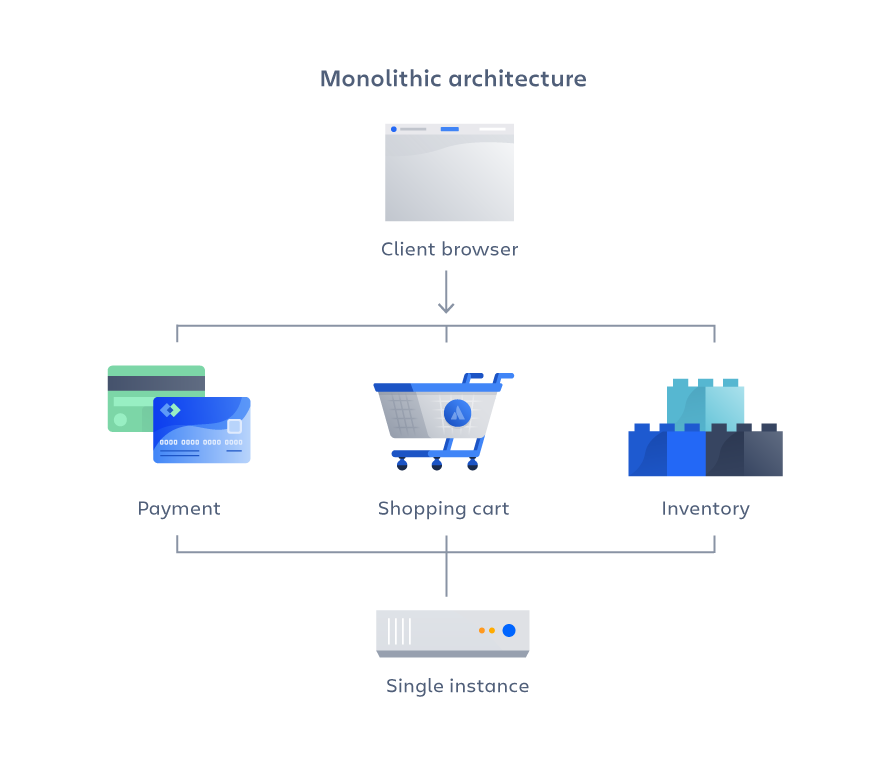
\includegraphics[width=1.0\textwidth]{images/monolithic-architecture-atlassian.png}
   \caption{Grafische Darstellung der monolithischen Architektur. 
   Unabhängig vom konkreten Anwendungsfall, ob jetzt Payment, Shopping Cart oder Inventory, gehören alle Services zu einer Instanz. \cite{website-atlassian-microservice-vs-monolothic}}
   \label{monolithic-arch-atlassian}
\end{figure}

In Abbildung \ref{monolithic-arch-atlassian} lässt sich hierbei erkennen, dass es zwar klar differenzierte Bereiche der Applikation, also zum Beispiel \enquote{Payment}, \enquote{Shopping cart} oder \enquote{Inventory} gibt, diese jedoch trotzdem zu einer einzigen Instanz gehören.

Zusammengefasst bietet eine monolithische Softwarearchitektur also folgende Vorteile:

\begin{itemize}
    \item Leichte Bereitstellung: Nur eine Applikation installieren zu müssen, erleichtert diesen Prozess enorm.
    \item Einfache Entwicklung: Da die Software übergreifend die gleichen Technologien verwendet, gestaltet sich die Entwicklung einfach.
    \item Einfaches Testing: Da die Applikation nur aus einem Teil besteht, lassen sich Tests mit einer höheren Abdeckrate leichter entwerfen.
\end{itemize}

Jedoch bietet diese Architektur auch die folgenden Nachteile:

\begin{itemize}
    \item Langsamere Entwicklung: Eine große, monolithische Applikation verlangsamt die Entwicklung, da der Quellcode immer größer und eventuell komplexer wird und, falls Änderungen in einem Modul getestet werden möchten, muss trotzdem die gesamte Applikation neu gestartet werden.
    \item Erschwerte Skalierung: Applikationen mit einer solchen Architektur können nur schwer großflächig skaliert werden.
    \item Verlässlichkeit und Fehlermanagement: Falls ein Fehler in einem Modul auftritt, könnte dies die restlichen Module der Applikation ebenso betreffen.
\end{itemize}


\textbf{Microservice Architektur}: Diese Softwarearchitektur ist eine relativ neue, jedoch höchst populäre Systemarchitektur. Dieses neue Modell steht laut Google Trends \cite{stats-google-microservice-trend} erst seit 2013 im Fokus, wird seitdem aber immer häufiger auch von Tech-Giganten wie Netflix, Amazon und Co. implementiert.
In der folgenden Grafik kann man das anfangs steigende Interesse sehr gut verfolgen:


\begin{figure}
  \centering
    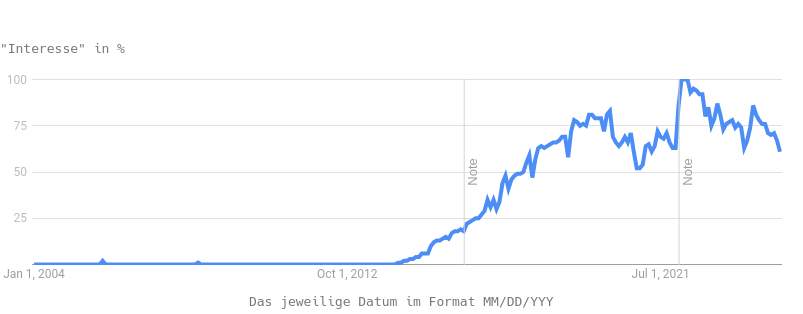
\includegraphics[width=1.0\textwidth]{images/stat-microservice-trend-google.png}
   \caption{Grafische Darstellung des Interesses der Google Benutzer während eines gewissen Zeitraums. \cite{stats-google-microservice-trend}}
   \label{stats-microservice-trend-google}
\end{figure}

Genauer gesagt ist die Microservice-Architektur ein Modell, welches sich auf viele kleine und unabhängige Service, statt eines großen Monolithen verlässt. Jeder dieser Services hat seine eigene Geschäftslogik, Datenbank und verfolgt ein eigenes Ziel.


\begin{figure}
  \centering
    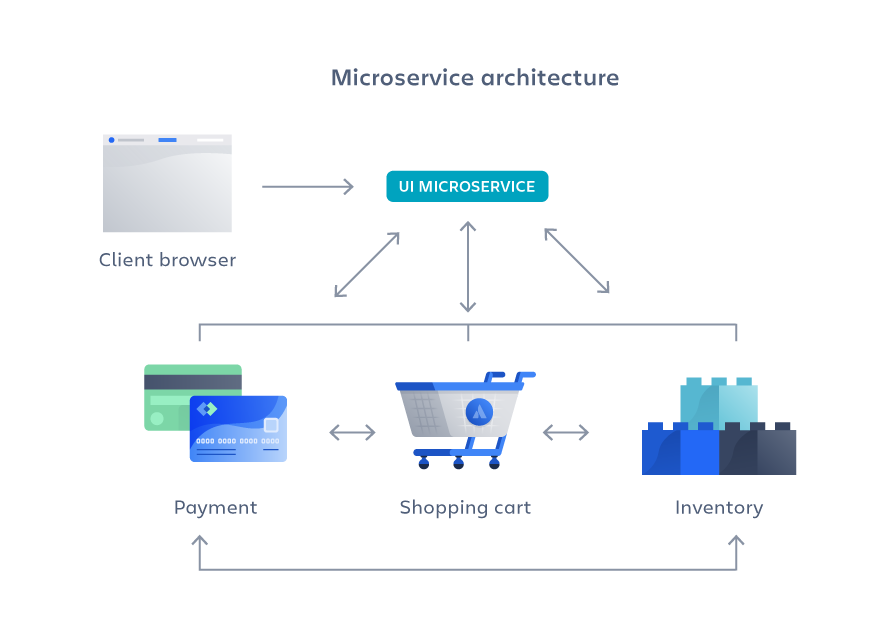
\includegraphics[width=1.0\textwidth]{images/microservice-architecture-atlassian.png}
   \caption{Grafische Darstellung der Microservice Architektur von \cite{website-atlassian-microservice-vs-monolothic}. Der Benutzer greift auf die Benutzeroberfläche zu, welche die einzelnen Services kontaktiert, damit diese dann zusammen die gewünschte Funktionalität ergeben.}
   \label{microservice-arch-atlassian}
\end{figure}

Letztendlich hat die Microservice-Architektur die folgenden Vorteile:

\begin{itemize}
    \item Flexible Skalierung: Wenn ein einzelner Microservice mehr Kapazitäten benötigt, da er vielleicht Ressourcen aufwendigere Aufgaben unternimmt, dann ist dies sehr einfach und kostengünstig möglich.
    \item Schnellere Entwicklung: Im Vergleich zu einer monolithischen Architektur ist die Entwicklung zwar komplexer, jedoch schneller, da Änderungen sofort implementiert und verteilt werden können.
    \item Flexible Wartung / Flexibles Fehlermanagement: Falls ein Service gewartet werden muss, oder möglicherweise ein Fehler bei einem Service auftritt, dann kann das Problem isoliert von den anderen Services behoben werden. Somit hat dies keinerlei Auswirkung auf die restlichen Komponenten der Applikation.
\end{itemize}

Jedoch bringt diese Architektur auch die folgenden Nachteile:

\begin{itemize}
    \item Erhöhte Komplexität: Viele verschiedene Microservices erhöhen die Komplexität einer Applikation und diese können, falls kein Auge darauf geworfen wird, auch komplett durcheinander und unordentlich miteinander kommunizieren. Dies kann sehr schnell sehr verwirrend werden.
    \item Erhöhte Kosten: Ob jetzt in der Entwicklung oder bei dem Deployment (\gls{deployment}); Microservices kosten mehr, da jeder einzelne Service seine eigene Umgebung, seine eigene Datenbank, etc. benötigt.
    \item Mangelhafter Standardisierung: Falls Microservices untereinander, zum Beispiel aufgrund von mangelnder Standardisierung der Protokolle, Schwierigkeiten haben, untereinander oder nach außen zu kommunizieren, erlöschen die meisten Vorteile der Architektur wieder.
\end{itemize}

\subsection{API-Entwicklung}

\subsubsection{Was ist eine API?}

Eine API (\gls{api}), in der deutschen Sprache auch Programmierschnittstelle genannt, ist eine Schnittstelle (\gls{interface}), welche verschiedene Teile einer Applikation miteinander verbindet. Man kann sich das so vorstellen: Wenn man in einem Restaurant speisen möchte, betritt man das Gebäude (in dem Fall: das Frontend). Danach kommt ein Kellner, nimmt die Bestellung auf und liefert diese zum Koch (in diesem Fall: das Backend). Wie hier schnell erkannt werden kann, ist der Kellner derjenige, der das Frontend und Backend miteinander verbindet; die Schnittstelle (siehe \cite{book-api-development-springer}).
\newline

Man unterscheidet hier, laut \cite{book-api-development-springer} S. 4 - 6, in \textbf{Client-API} und \textbf{Server-API}:
\newline


Eine \textbf{Client-API} ist eine Schnittstelle, die es einer Anwendung ermöglicht, mit dem Server zu kommunizieren, oft über HTTP-Anfragen (z. B. REST, GraphQL). Sie wird im Frontend verwendet, um Daten vom Server abzurufen oder zu senden und reagiert in Echtzeit auf Benutzeraktionen.


Eine \textbf{Server-API} hingegen stellt serverseitig Funktionen und Daten bereit, auf die der Client zugreifen kann. Sie verarbeitet Anfragen, führt Logik aus (z. B. Datenbankoperationen) und liefert strukturierte Antworten zurück, die der Client dann verwendet. Sie bildet also das Backend und steuert den Großteil der Geschäftslogik. 

Nun gibt es noch gewisse Standards, welche in der Softwareentwicklung verwendet werden.

\subsubsection{\gls{soap}}

Als das Internet noch am Anfang stand, gab es noch keine richtigen standardisierten Methoden, homogene (\gls{homogen}) Integration von Applikationen zu ermöglichen. 
Denn zu der Zeit liefen die meisten Applikationen im Internet über das \textbf{SOAP} (\gls{soap}), welches ein einfaches Netzwerkprotokoll, verantwortlich für den Austausch von Daten zwischen Systemen sowie Durchführung von RPC (\gls{rpc}), war.

Dieses Netzwerkprotokoll brachte aus der heutigen Sicht einige Nachteile mit sich, welche in \cite{paper-soap} erläutert werden:

\begin{itemize}
    \item Hohe Komplexität: das Protokoll ist sehr komplex, da es auf XML (\gls{xml}) basiert und eine strikte Struktur mit umfangreichen Regeln und Standards erfordert. Dadurch ist die Technologie schwerfällig und kompliziert, sowohl in der Implementierung, als auch in der Wartung.
    \item Overhead: Kommunikationen über SOAP erzeugen viel Overhead, da die Nachrichten viele XML-Tags und umfangreiche Header enthalten. Dies führt zu größeren Datenmengen und damit zu einer langsameren Übertragung.
    \item Aufwendige Integration: Das Protokoll lässt sich nur mit viel Aufwand von modernen Technologien, wie z.B. JavaScript, integrieren, was den Entwicklungsaufwand erhöht.
\end{itemize}

\subsubsection{\gls{rest}}

\textbf{Die Geschichte von REST}

Um nun den älteren \gls{soap}-Standard abzulösen, wurde REST eingeführt. Dieser Standard wurde von Roy T. Fielding in seiner Doktorarbeit Architectural Styles and the Design of Network-Based Software Architectures, siehe \cite{doktorarbeit-rest}, bei der University of Californa im Jahr 2000 erfunden. 


Die REST Architektur ermöglichte es, über das Internet mit jedem Server über das HTTP-Protokoll zu kommunizieren, weshalb man diesen Standard sowohl überall im Internet, als auch im eigenen internen Netzwerk, verwenden kann. 


Als erstes versuchte sich eBay an der Architektur. Nach einem erfolgreichen Gelingen zogen Firmen wie Amazon Web Services, Facebook, Twitter und Google nach. Heutzutage ist es relativ schwierig, eine Applikation ohne REST-API zu finden. Siehe \cite{book-modern-api-development-packt} S. 26.
\newline


 \textbf{Grundlagen von REST}

 Grundsätzlich arbeitet REST mit dem Prinzip, dass alles eine Ressource ist und über einen eindeutigen \gls{url} identifizierbar ist. Dazu zählen z.B. Benutzer, Artikel, etc.

 Da REST ebenso auf dem HTTP-Protokoll basiert, kann man über die folgenden Methoden mit den einzelnen Ressourcen interagieren (siehe \cite{book-modern-api-development-packt} S. 31 - 33):

 \begin{itemize}
     \item \textbf{GET}: Mit dieser Methode lassen sich Daten von der API abrufen. Durch eine URL wie zum Beispiel \textsc{https://server.com/api/user/1} könnte zum Beispiel ein Benutzer mit der id=1 abgerufen werden.
     \item \textbf{POST}: Mit dieser Methode lassen sich über die Schnittstelle neue Daten erstellen. Hier sind die eigentlichen Daten im sogenannten \gls{req-body} untergebracht. Dies kann z.B. eine Anfrage sein, welche ein vom Benutzer ausgefülltes Formular an einen Server sendet.
     \item \textbf{PUT}: Hier können wir bestehende Daten aktualisieren. Das Prinzip ist dasselbe wie bei einer POST-Anfrage, nur mit dem Unterschied, dass eine PUT-Anfrage \gls{idempotent} ist.
     \item \textbf{DELETE}: Mit dieser Methode können Ressourcen auf einem Server gelöscht werden.
 \end{itemize}

Neben den HTTP-Methoden haben \gls{restful-app} fünf Grundprinzipien, welche bei der eigenen Implementierung beachtet werden müssen, um von allen Vorteilen der Architektur profitieren zu können:

\begin{enumerate}
    \item \textbf{Uniform Interface:} Dieses Prinzip gewährleistet eine einheitliche und standardisierte Kommunikation zwischen Client und Server. Es umfasst vier Unterprinzipien (Prompt \cite{prompt-gpt-rest}):
    \begin{enumerate}
        \item \textit{Ressourcenidentifikation:} Jede Ressource wird durch eine eindeutige URI (Uniform Resource Identifier) identifiziert.
        \item \textit{Manipulation durch Repräsentationen:} Clients interagieren mit Ressourcen über deren Repräsentationen, wie JSON oder XML.
        \item \textit{Selbstbeschreibende Nachrichten:} Jede Nachricht enthält ausreichend Informationen, damit der Empfänger sie verstehen und verarbeiten kann.
        \item \textit{\gls{hateoas}:} Clients navigieren durch die Anwendung mittels Hyperlinks, die in den Antworten enthalten sind, siehe \cite{book-modern-api-development-packt} S. 34 - 37.
    \end{enumerate}

    \item \textbf{Cacheable:} Serverantworten sollten Informationen enthalten, die angeben, ob die Antwort vom Client gecacht werden kann. Dies verbessert die Effizienz, reduziert die Serverlast und minimiert die Latenz, indem unnötige Anfragen vermieden werden.

    \item \textbf{Layered System:} Die Architektur ist in Schichten unterteilt, wobei jede Schicht eine spezifische Funktion erfüllt. Clients interagieren nur mit der unmittelbar benachbarten Schicht und sind sich der anderen Schichten nicht bewusst. Dies erhöht die Flexibilität und Skalierbarkeit des Systems.

    \item \textbf{Client-Server}: Dieses Prinzip definiert zwei Aktoren in der Applikation: einen Client und einen Server. Hierbei fragt der Client Informationen vom Server ab (oder möchte eine solche auf dem Server speichern) und tut dies mittels HTTP-Anfragen. Der Server ist dafür zuständig, diese Anfragen vom Client zu empfangen, zu verarbeiten und dem Client eine Antwort zuzusenden.
    \item \textbf{Stateless}: Dies bedeutet, dass, anhand \cite{book-modern-api-development-packt} S. 27, der Server keinen Status von keinem Client  sammelt und verfolgt. Die Anfrage von einem Client muss also alle Informationen beinhalten, welche für das Abarbeiten des Anliegens benötigt werden. Dies verschafft einem bei der Implementierung den Vorteil, dass das System sehr simpel ist; HTTP-Anfragen laufen komplett isoliert voneinander ab.
\end{enumerate}
 

\subsubsection{GraphQL}

\textbf{Die Geschichte von GraphQL}

Vor 13 Jahren, im Jahr 2011, stieß Facebook auf ein Problem: Sie wollten eine performante Mobile Applikation entwickeln, jedoch fehlte ihnen die Technologie dazu. Zu dieser Zeit gab es zwar schon den REST-Standard, jedoch war dieser für die enorme Datenmenge, welche Facebook generierte, einfach nicht ausgelegt. Damals lag die durchschnittliche Internetbandbreite im kB/s-Bereich, weshalb die Firma mit einer performanteren API schnell den Markt erobern würde.

Im Jahr 2012 setzten sich ein paar Facebook-Ingenieure, Lee Byron, Dan Schafer und Nick Schrock, zusammen und entwickelten \textbf{GraphQL}. Rasend schnell breitete sich diese neue Technologie auf die gesamte Firma aus. 

Nach ein paar Jahren der eigenen Verwendung beschloss Facebook, den Quellcode der Technologie für jedermann bereitzustellen. Damit ermöglichten sie die Integration der Softwarearchitektur in sämtlichen bereits bestehenden Technologien, was unter \cite{book-modern-api-development-packt} S. 479 zu finden ist.
\newline

\textbf{REST versus GraphQL im Vergleich}

Grundsätzlich ist GraphQL performanter, flexibler und effizienter als REST.

Denn an sich funktioniert die Architektur so, dass man nicht unzählige \gls{endpoints} für jeden Zweck erstellen muss, sondern die Parameter, welche man von einem Server erfüllt haben möchte, bei einer Anfrage setzen kann.

Möchte man sich jetzt zum Beispiel als Benutzer bei einem Online-Shop anmelden, wobei man nach der Anmeldung zu der Produkt-Seite weitergeleitet wird, ist dies zwar ein Prozess, jedoch müsste man hier bei der REST-Architektur mindestens drei Endpoints implementieren:

\begin{enumerate}
    \item \textbf{Benutzer-Endpoint}: Um die Benutzerdaten zu laden.
    \item \textbf{Produkt-Endpoint}: Um die Produkte zu laden.
    \item \textbf{Einkaufswagen-Endpoint}: Um mögliche Gegenstände aus dem Einkaufswagen des Benutzers zu laden.
\end{enumerate}

All dies ist mit GraphQL nicht notwendig: Hier kann man, anhand der Untersuchung in \cite{book-modern-api-development-packt} S. 480 - 481, dem Server ganz einfach sein Vorhaben schildern, und dieser wird dies dann mit einer Anfrage erfüllen.

\subsubsection{API Sicherheit}

Da diese Schnittstellen elementar für moderne Applikationen sind, stellen sie besonders attraktive Ziele für potenzielle Angreifer dar. Um das Stehlen von Daten und/oder die Übernahme des Servers aufgrund einer Schwachstelle in der Applikation zu verhindern, gibt es gewisse Sicherheitsmaßnahmen, die man setzen kann.

\textbf{Arten von möglichen Angriffen}

Es gibt unzählige Wege, sich selbst Zugang zu einem System zu verschaffen; die beliebtesten sind, laut dem Paper \cite{paper-enterprise-api-security-and-gdpr-compliance} S. 3, die folgenden:

\begin{itemize}
    \item \textbf{Script Insertion}: Eine solche Attacke hat das Ziel, Quellcode auf ein Serversystem zu schmuggeln, mit dem Sinn, dass dieser bösartige Code dann auf diesem System ausgeführt wird. Als Beispiel dafür würde zum Beispiel die Eingabe von JavaScript Quellcode bei einem normalen Formular dienen.
    \item \textbf{SQL injections}: Bei diesem Angriff nutzt der Angreifer ebenso eine Schwachstelle bei der Datenübermittlung an den Server aus. Hierfür muss der Server über eine \gls{sql} Datenbank verfügen. Das Ziel ist es, die Datenbankabfrage so zu verändern, dass zum Beispiel bei der Ausgabe Daten angezeigt werden, die eigentlich nicht abgefragt wurden.
    \item \textbf{Bounds or buffer overflow attacks}: Diese Art von Angriff hat das Ziel, dem Server so viele Daten zu senden, bis das System zusammenstürzt. Hier sprengt die unerwartet große Datenmenge quasi den Rahmen des Systems. 
\end{itemize}

Um diesen Angriffen standhalten zu können und die generelle Sicherheit der eigenen Schnittstelle zu verbessern, kann man folgende Sicherheitsstrategien implementieren (siehe \cite{paper-enterprise-api-security-and-gdpr-compliance} S. 4):

\begin{itemize}
    \item \textbf{Access control management}: Dieser Mechanismus beschäftigt sich damit, den Zugriff der einzelnen Benutzer auf die API zu limitieren. Das heißt, dass man jedem Benutzer einen eindeutigen Schlüssel zuweist, mit dem er sich bei jeder Anfrage ausweisen muss. Somit ist (1) jeder Zugriff auf die API verifizierbar und (2) die Auslastung der Ressourcen unter Kontrolle, da man hier die jeweiligen Benutzer in der Verwendung der Schnittstelle limitieren kann.
    \item \textbf{Client-throttling}: Diese Methode ist ähnlich zum \textbf{Access control management}, bietet jedoch den Vorteil, dass man hier keine registrierten Benutzer benötigt. Hier wird einfach nur jeder Client in der Benutzung der Schnittstelle limitiert. Zum Beispiel kann man dies so konfigurieren, dass jeder Client (z.B. identifizierbar anhand einer IP-Adresse oder einer zugewiesenen temporären \gls{uuid}) die Schnittstelle nur 100-mal pro Minute aufrufen kann. Dies verhindert \gls{ddos} Angriffe.
    \item \textbf{API Gateways Security}: Ein sogenanntes \textit{API Gateway} ist ein wichtiger Bestandteil einer sicheren Schnittstelle. Dieses fungiert als Verkehrspolizei der API Schnittstelle und kontrolliert, ob Anfragen legitim sind, indem es den Benutzer (Autorisierung), den Inhalt und verschiedenste Parameter überprüft. Solch ein Mechanismus verschlüsselt ebenso kritische Daten und verhindert, dass geschützte Daten in System-Logs gelangen. 
    \item \textbf{Communication Security}: Um die Kommunikationssicherheit zu gewährleisten, verwendet man das \gls{tls-ssl} Protokoll. Der TLS Standard wird dazu verwendet, um eine sichere Verbindung zwischen zwei Endpunkten (in diesem Fall dem Client und dem Server) herzustellen. Er stellt sicher, dass jegliche Kommunikation verschlüsselt bleibt. Eine REST-API verwendet HTTP und wird damit von TLS unterstützt.  
\end{itemize}

Diese Mechanismen haben den Sinn und Zweck, den Zugriff auf die API strengstens zu kontrollieren.

\subsection{Ergebnis der Literaturrecherche}

Diese Ausarbeitung verdeutlicht die wesentlichen Prinzipien und Technologien, die für eine erfolgreiche Backend- und API-Entwicklung entscheidend sind. Die Analyse verschiedener Architekturmodelle hat gezeigt, dass die Wahl der richtigen Struktur je nach Projektanforderung maßgeblich zur Effizienz und Skalierbarkeit beiträgt. Ebenso bieten moderne API-Standards wie REST und GraphQL flexible und performante Möglichkeiten, um eine reibungslose Kommunikation zwischen den einzelnen Komponenten zu gewährleisten.
\newline

Die Untersuchung hat auch aufgezeigt, dass die Integration moderner Sicherheitsmechanismen und die effiziente Verarbeitung von Formulardaten im Hintergrund entscheidend sind, um eine stabile und sichere Plattform bereitzustellen. Insgesamt bietet diese Recherche eine solide Basis, um die Entwicklungsziele des Projekts zu verwirklichen und die zentrale Forschungsfrage zu beantworten.
\setauthor{Sebastian Sailer}
\section{Entwicklung der Datenbank}

\subsection{Einleitung}

Das Ziel dieses Projektes ist die Konzeptionierung und Verwaltung einer Datenbank, sowie die Automatisierung von Abläufen, um periodisch Buchungsprotokolle zu erstellen, und den Mitarbeitern der beauftragenden Firma zur Verfügung zu stellen.
\newline
Um diese Ziele zu erreichen, benötigt die Anwendung eine effiziente und \gls{Persistenz} Art, um Daten zu speichern.
\newline
Daraus lässt sich folgende zentrale Forschungsfrage ableiten:\vspace{5mm}\newline
\indent \textbf{Wie können Buchungsdaten so gespeichert und zugänglich gemacht werden, dass der \indent Zugriff sowohl benutzerfreundlich als auch effizient ist?}

\vspace{3mm}\noindent Um diese Frage effektiv beantworten zu können, ist es nötig, die aktuell bewährten Methoden für Datenspeicherung zu analysieren. Diese Untersuchung wird sich aufgrund der Vielzahl an Ansätzen auf die für die Applikation wichtigsten Methoden konzentrieren.


\subsection{Datenbanksysteme}
Ein Datenbanksystem besteht aus einem Datenbankmanagementsystem (DBMS) und einer oder mehreren Datenbanken. Ein DBMS umfasst die Softwaremodule, die für die Verwaltung der Datenbank zuständig sind, während die Datenbank selbst lediglich den strukturierten Datenbestand darstellt.

 \vspace{3mm}\noindent \textit{"Die klassischen Einsatzgebiete der Datenbanken sind Anwendungen im kommerziellen Bereich, die sich aus Buchhaltungs- und Katalogisierungsproblemen entwickelt haben"}-\cite{Buch:GunterSaake} S.10 Einsatzgebiete und Grenzen 
 

 \vspace{3mm}\noindent Dies sind jedoch nicht die einzigen Einsatzmöglichkeiten von Datenbanksystemen. Grundsätzlich werden Datenbanken überall dort eingesetzt, wo Daten gespeichert und organisiert werden müssen.
 
 \vspace{3mm}\noindent Hierbei wird zwischen zwei Kategorien unterschieden:
 
 \begin{itemize}
    \item \textit{RDBMS} - relationale Datenbankmanagementsysteme
    \item \textit{NoSQL} - Not Only \gls{SQL} 
 \end{itemize}
 
\vspace{3mm}\noindent Bevor mit der Implementierung eines spezifischen DBMS begonnen wird, ist es essenziell, diese Kategorien eingehend zu verstehen.
\cite{Buch:GunterSaake} \textit{Datenbanken, Konzepte und Sprachen S.10}

\newpage
\subsection{Relationales DBMS}
Laut \textit{\cite{Buch:EdwinSchicker} S.57, Relationale Datenbanken} bestehen Relationale Datenbankmanagementsysteme ausschließlich aus Tabellen, über die auf Daten zugegriffen wird. Der Aufbau einer solchen Datenbank kann durch das Hinzufügen von Zeilen und Spalten flexibel angepasst werden. Die Verknüpfungen zwischen den Tabellen werden über Beziehungen hergestellt, die ebenfalls in den Tabellen gespeichert sind. \newline 

\vspace{3mm}\makefig{images/erDiagramm.png}{height=5cm}{Ein einfaches Objekt-Diagramm, wobei 1 Schüler, n viele Bücher ausborgen kann}{fig:caption-label}

\noindent Das Diagramm in Abbildung 4.4 zeigt eine Beispielbeziehung zwischen Studenten und Büchern in einem Bibliothekssystem. Ein Student, beschrieben durch \textbf{Ausweisnummer}, \textbf{Vorname} und \textbf{Nachname}, kann mehrere Bücher ausleihen, während jedes Buch, gekennzeichnet durch \textbf{Name} und \textbf{Artikelnummer}, einem Leihvorgang zugeordnet ist. Die \textbf{1:n-Beziehung} „\textbf{leiht aus}“ verdeutlicht den Prozess der Buchausleihe durch Studenten.


\subsubsection{ACID}

\vspace{3mm}\noindent Darüber hinaus erfüllen relationale Datenbankmanagementsysteme meistens die vier Eigenschaften des ACID-Prinzips, siehe \textit{\cite{Buch:GunterSaake} S.374}.

\begin{itemize}
    \item \textbf{Atomicity}: Eine Transaktion wird entweder vollständig oder gar nicht ausgeführt. Wenn eine Transaktion fehlschlägt, werden alle vorherigen Änderungen rückgängig gemacht.
    \item \textbf{Consistency}: Eine Transaktion bringt das System von einem gültigen Zustand in einen anderen gültigen Zustand, unter Wahrung aller definierten Integritätsbedingungen.
    \item \textbf{Isolation}: Transaktionen werden so ausgeführt, als ob sie alleine ablaufen, d.h. parallele Transaktionen beeinflussen sich nicht gegenseitig.
    \item \textbf{Durability}: Nach dem Abschluss einer Transaktion sind die Änderungen permanent, auch im Falle eines Systemabsturzes.
\end{itemize}
Wie \cite{Paper:performanceComparison} beschreibt, weisen auch Relationale Datenbanken Nachteile auf, wie etwa erhöhte Laufzeiten und hohe Ein-/Ausgabeanforderungen bei Zugriffen über mehrere Tabellen. Zudem erfordert die Speicherung bestimmter Daten eine gewisse \gls{Redundanz}. Ebenso sind sie bei einer großen Anzahl an Daten langsamer bei \gls{CRUD} Operationen. 


\subsubsection{BASE}

\noindent Das BASE-Modell wird oft als Alternative zu ACID in verteilten Datenbanksystemen verwendet und stellt eine weniger strikte Konsistenz sicher, um bessere Verfügbarkeit und Partitionstoleranz zu erreichen. NoSQL DBMS verwenden in der Regel dieses Konzept. BASE steht hierbei für:

\begin{itemize}
    \item \textbf{Basically Available}: Das System garantiert Verfügbarkeit, auch wenn nicht immer auf die neuesten Daten zugegriffen werden kann.
    \item \textbf{Soft State}: Der Zustand des Systems kann sich über die Zeit ohne externe Eingriffe ändern, da es zu Verzögerungen bei der Konsistenz kommen kann.
    \item \textbf{Eventual Consistency}: Das System wird über die Zeit schließlich konsistent, aber es kann Phasen geben, in denen nicht alle Knoten die gleichen Daten haben.
\end{itemize}

\subsubsection{CAP}

\noindent Das CAP-Theorem besagt jedoch, dass ein verteiltes Datenbanksystem maximal zwei der folgenden drei Eigenschaften gleichzeitig erfüllen kann:

\begin{itemize}
    \item \textbf{Consistency (Konsistenz)}: Alle Knoten eines verteilten Systems sehen die gleichen Daten zur gleichen Zeit.
    \item \textbf{Availability (Verfügbarkeit)}: Jedes Anfrage erhält immer eine Antwort (entweder den aktuellen Zustand der Daten oder einen Fehler).
    \item \textbf{Partition Tolerance (Partitionstoleranz)}: Das System funktioniert auch dann weiter, wenn Teile des Netzwerks ausfallen oder nicht kommunizieren können. Die einzelnen Partitionen sind dann ein eigenes System, bis sie wieder synchronisiert werden.
\end{itemize}

\noindent Das CAP-Theorem zwingt Datenbankarchitekten, eine Abwägung zwischen diesen Eigenschaften zu treffen. In Abbildung 4.5 wird gezeigt, welche Möglichkeiten es dabei gibt.

\makefig{images/CapTheorem.png}{height=5cm}{Die 3 Möglichkeiten bei CAP \cite{Buch:AndreasMaier} S.149 }{fig:caption-label}

\vspace{3mm}\noindent Die Quelle \cite{Buch:AndreasMaier} \textit{S. 148} beschreibt, dass im Gegensatz zu ACID, BASE eine zeitliche  Synchronisierung ermöglicht. Das ist besonders bei verteilten und webbasierten Systemen vorteilhaft.\newline


\newpage
\subsubsection{NoSQL DBMS}
\enquote{Not only SQL} (früher No SQL) verwenden kein relationales Modell, sondern ein flexibles Schemamodell, das unterschiedliche unstrukturierte Datentypen wie Dokumente, Schlüssel-Wert-Paare, breite Spalten und Graphen unterstützt. Die Vorteile solcher DBMS sind Flexibilität, hohe Leistung, horizontale Skalierbarkeit und eine einfache Entwicklung. 

\vspace{3mm}\noindent Es gibt fünf Haupttypen, zwischen denen unterschieden wird:
\vspace{3mm}\begin{itemize}
    \item \textbf{Dokumentendatenbanken:} Die Daten werden in einem JSON-ähnlichen Format gespeichert, das den Datenstrukturen entspricht, die Entwickler in ihrem Anwendungscode verwenden. Dokumentdatenbanken werden häufig für Blogging-Plattformen, E-Commerce, Echtzeitanalysen und Content-Management-Systeme verwendet.
    
    \item \textbf{Datenbanken mit Schlüssel/Wert-Paaren:} Jeder Schlüssel ist mit einem Wert wie einem String, einer Zahl oder einem komplexen Objekt verknüpft. Diese Struktur wird häufig für Nutzereinstellungen, Einkaufswagen und Profile in Webanwendungen verwendet, wobei der Schlüssel zum Speichern oder Abrufen des zugehörigen Werts dient, ohne dabei die ganze Datenbank durchgehen zu müssen.
    
    \item \textbf{Spaltenorientierte Datenbanken} speichern Daten in Spalten anstelle von Zeilen und ermöglichen so eine flexiblere Speicherung innerhalb einer Tabelle. Diese Struktur eignet sich besonders für Analyseanwendungen, bei denen einzelne Spalten schnell abgefragt und aggregiert werden müssen. Sie werden häufig für Kataloge, Betrugserkennung und Empfehlungssysteme verwendet, da sie eine schnelle Datenabfrage ermöglichen.
    
    \item \textbf{Graphdatenbanken} organisieren Daten als Knoten in einem Diagramm und betonen die Beziehungen zwischen diesen Knoten. Verbindungen (Kanten) werden als zentrale Elemente gespeichert, was eine einfachere Navigation und eine tiefere Darstellung der Beziehungen ermöglicht. Sie sind besonders nützlich in Systemen, die komplexe Beziehungen abbilden, wie Social Media und Reservierungssysteme.
    
    \item \textbf{In-Memory-Datenbanken} speichern Daten im Arbeitsspeicher, wodurch sie niedrige Latenzzeiten für Echtzeitanwendungen bieten. Diese Datenbanken werden vor allem für Caching, Messaging, Streaming und Echtzeitanalysen eingesetzt. Sie ermöglichen schnelle Datenzugriffe und werden oft in Szenarien genutzt, in denen Geschwindigkeit und geringe Verzögerung entscheidend sind.
    
\end{itemize}
\cite{Google:NoSQL} \textit{Google Dokumentation zu NoSQL} \newline
\cite{Buch:AndreasMaier} \textit{SQL- \& NoSQL-Datenbanken S.18}
\newpage
\subsection{Geschichte von Datenbanken}

Nachdem wir nun die Grundlagen eines Datenbanksystems kennen, widmen wir uns seiner Entstehung. Laut der Definition von Oxford Languages ist eine Datenbank ein 
\textit{\enquote{System zur Beschreibung, Speicherung und zum Abrufen von großen Datenmengen}} \cite{Definition:Datenbank}

\noindent Datenbanken existieren jedoch nicht erst seit der Einführung des Computers. Bereits lange zuvor gab es sie schon etwa in Form von Bibliotheken, Geschäfts- und Krankenakten oder Ähnlichem. Einige der damals entwickelten Konzepte werden bis heut angewandt.

\vspace{3mm}\noindent \textit{Es folgt eine Zusammenfassung aus verschiedenste Paper, die ihre Quellen am Ende des Absatzes angegeben hat.}

\vspace{3mm}\noindent \textbf{1960er Jahre -}
Als es in den 1960er Jahren Computer immer verbreiteter wurden, begann auch der Einsatz von Datenbanken zur Speicherung großer Datenmengen. Die Einführung von Direktzugriffsspeichern (wie Festplatten) ermöglichte den Übergang von batch-Systemen, zu interaktiven Systemen. Es wurden zwei Modelle entwickelt, das hierarchische Modell (Information Management System, IMS von IBM) und das Netzwerkmodell (CODASYL). Anwendungen griffen über Zeiger auf die Daten zu, was komplexe Navigationsstrukturen erforderte, aber Flexibilität beim Zugriff bot. Ein bedeutendes System dieser Zeit war SABRE, entwickelt von IBM für American Airlines zur Verwaltung von Flugreservierungen.  \cite{Paper:Geschichte3} \cite{Paper:Geschichte4} \cite{Paper:Geschichte1}

\vspace{3mm}\noindent \textbf{1970er Jahre -}
 1970 veröffentlichte E.F. Codd das relationale Datenbankmodell, das einen \newline\gls{Paradigmenwechsel} verursachte. Das Modell schlug die Suche nach Daten über Inhalt anstatt über Zeiger vor. Codds Modell, basierend auf relationaler Algebra, ermöglichte eine klarere Datenstruktur und inspirierte die Entwicklung von \gls{System R} bei IBM. Relationale Datenbanken setzten sich zunehmend durch, und IBM entwickelte \gls{SQL}  als eine benutzerfreundliche Sprache, um diese Modelle zu verwalten.
\cite{Paper:Geschichte1}\cite{Paper:Geschichte2}

\vspace{3mm}\noindent \textbf{1980er Jahre -}
Relationale Datenbanken gewannen zunehmend an Popularität, und SQL wurde zum Standard für die Abfrage und Verwaltung relationaler Daten. Die Markteinführung kommerzieller Systeme wie IBM DB2 und Oracle trug dazu bei, relationale Datenbanken zum Standard in der Datenverarbeitung zu machen. 
\cite{Paper:Geschichte1}\cite{Paper:Geschichte4}

\vspace{3mm}\noindent \textbf{1990er Jahre -}
  Um den Anforderungen an größere, komplexere Daten und die Integration mit Netzwerken gerecht zu werden, entwickelten sich Datenbanktechnologien weiter. Objektorientierte Datenbanksysteme wurden eingeführt. Die zunehmende Nutzung des Internets führte zu Anforderungen an leistungsfähige und webfähige Datenbanken.
  \cite{Paper:Geschichte4}

\vspace{3mm}\noindent \textbf{2000er Jahre bis heute -}
Mit der zunehmenden Bedeutung des Internets wurden skalierbare und verteilte Datenbanken wie NoSQL populär, um große und einheitliche Datenmengen zu verarbeiten. SQL-basierte relationale Datenbanken bleiben jedoch weiterhin ein wesentlicher Standard in der Geschäftswelt. \cite{Paper:Geschichte4}
 

\subsection{Ergebnis der Literaturrecherche}
Die Recherche zeigt, dass ein relationales Datenbanksystem die beste Wahl für die Datenspeicherung in diesem Projekt ist. Die Analyse verdeutlicht, dass eine relationale Datenbank in Bezug auf Effizienz, Skalierbarkeit und Benutzerfreundlichkeit, bei den benötigen Daten, besonders geeignet ist. Zudem bieten relationale Datenbanken eine große Auswahl an Datenbankmanagementsystemen, was die Auswahl eines passenden Systems erleichtert.

\setauthor{Sebastian Pollak}
 \section{Entwicklung des Formularsystems}

\subsection{Einleitung}

Das Projekt umfasst die strukturierte und DSGVO-konforme Erfassung von Gästedaten mittels einer benutzerfreundlichen Webanwendung für Mieter. Im Fokus steht die Entwicklung eines intuitiven und länderspezifischen Formularsystems, das die Vollständigkeit und Validierung der erfassten Daten sicherstellt, bevor diese an das Backend geliefert werden.
Daraus ergibt sich folgende zentrale Forschungsfrage:

\begin{quote}
\textbf{Wie kann die Erfassung und Verarbeitung von Formulardaten in einer Webanwendung gestaltet werden, sodass die Eingabe effizient, sicher und benutzerfreundlich gewährleistet wird?}
\end{quote}

Das Beantworten dieser Frage setzt die Analyse der derzeitig gängigen Ansätze zur Datenvalidierung und zum Interface-Design voraus. Diese Analyse wird sich hauptsächlich mit der Theorie dieser Ansätze auseinandersetzen.

\subsection{Grundlagen von Formularsystemen}
\subsubsection{Definition und Zweck eines Formulars}
Wie auf Seite zwei des Artikels ''An extensive guide to web form usability'' \cite{mifsud2011extensive} definiert sind Formulare strukturierte Schnittstellen zur Datenerfassung und anschließender Übertragung zwischen Benutzer und Systemen. Sie bestehen im Normalfall aus folgenden Komponenten: \cite{prompt2_pollak}

\begin{enumerate}

    \item \textbf{Labels/Beschriftungen} Sie geben dem Benutzer Kontext und Anweisungen für jedes Eingabefeld.
    
    \item \textbf{Eingabefelder} Eingabefelder ermöglichen, dem Benutzer Informationen bereitzustellen. Dies beinhaltet Textfelder, Passwortfelder, Kontrollkästchen, Optionsschaltflächen, Schieberegler und mehr.
    
    \item \textbf{Action} Aktionen geben dem Benutzer die Möglichkeit, mittels eines Buttons oder Links eine Aktion durchzuführen, wie zum Beispiel das Absenden des Formulars.

    \item \textbf{Help} Die Hilfefunktion soll den Benutzer dabei unterstützen, das Formular korrekt auszufüllen, indem sie beispielsweise eine Erklärung zu einem Eingabefeld liefert, wie in Abbildung \ref{fig:abbildung2} dargestellt.
    
    \item \textbf{Messages} Nachrichten geben dem Benutzer Rückmeldung basierend auf seinen Eingaben. Diese können positiv sein (zum Beispiel, dass das Formular erfolgreich übermittelt wurde) oder negativ („Der von Ihnen gewählte Benutzername ist bereits vergeben“).

    \item \textbf{\gls{form-validation}} Das Validieren der Daten stellt sicher, dass die vom Benutzer übergebenen Daten den Akzeptanzkriterien entsprechen. Auf Datenvalidierung wird im Kapitel \ref{datenvaliderung} genauer eingegangen.
    
\end{enumerate}

\begin{figure}
    \centering
    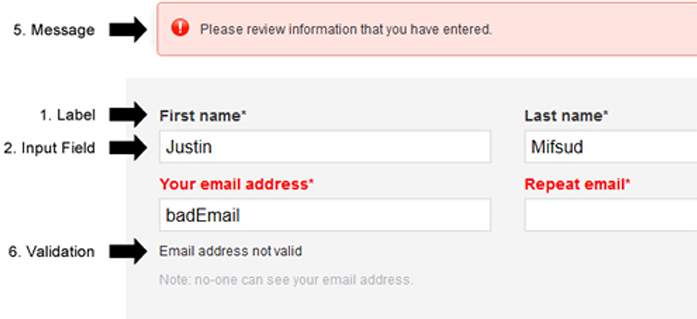
\includegraphics[width=0.75\linewidth]{images/formularKomponenten1.png}
    \caption{Formularkomponenten 1 \cite{mifsud2011extensive}}
    \label{fig:abbildung1}
\end{figure}

\begin{figure}
    \centering
    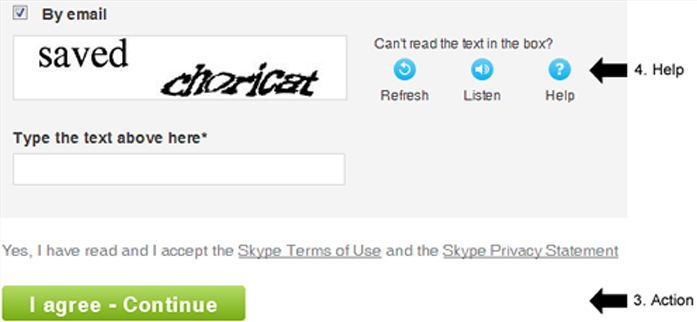
\includegraphics[width=0.75\linewidth]{images/formularKomponenten2.png}
    \caption{Formularkomponenten 2 \cite{mifsud2011extensive}}
    \label{fig:abbildung2}
\end{figure}

Wie im ersten Kapitel des Buches ''Web form design: Filling in the blanks'' \cite{wroblewski2008web} nachgelesen werden kann, bieten Formulare sowohl aus der Perspektive des Benutzers als auch des Anbieters allerlei Vorteile. Sie steigern generell die Effizienz und verbessern die \gls{usability}. Sie strukturieren Daten in einem vordefinierten Format und leiten die Benutzer bei guter Gestaltung effektiv durch den Eingabeprozess. Ebenso wird, wie oberhalb erwähnt, die Integrität der Daten sichergestellt, was wichtig ist, um eine potenzielle Prozessautomatisierung zu ermöglichen.

\subsubsection{Historische Entwicklung}
Die Geschichte der Formulare beginnt mit handgeschriebenen Dokumenten auf Papier. Diese frühen Formulare dienten der strukturierten Erfassung von Informationen, um Verwaltungsprozesse zu optimieren. Nachdem in den 1990er Jahren das World Wide Web mit statischen Seiten entstanden war, wuchs der Wunsch der Nutzer, aktiv zu interagieren und nicht nur Informationen zu konsumieren. Infolgedessen wurden die oben beschriebenen Formulare entwickelt. Diese ermöglichten dann erstmals die Datenerfassung über den Webbrowser. Dies beschreiben Caroline Jarrett und Gerry Gaffney in ihrem Buch ''Forms that work: Designing web forms for usability'' \cite{jarrett2009forms}. \cite{prompt3_pollak}

\subsection{\gls{usability} und Formulardesign}
\subsubsection{Warum ist das Formulardesign wichtig?}
Formulare stehen immer zwischen dem Ziel des Benutzers und den Zielen der Firmen. Beispielsweise möchten Kunden auf E-Commerce-Websites Dinge kaufen, die sie brauchen, und das Unternehmen möchte den Umsatz maximieren. Im Weg steht dabei das Checkout-Formular.
Daher ist es in diesem Beispiel wichtig, das Checkout-Formular besonders benutzerfreundlich zu gestalten. Wie im ersten Kapitel des Buches ''Web form design: Filling in the blanks'' \cite{wroblewski2008web} aufzeigt, kann durch diese Optimierung die Anzahl erfolgreich abgeschlossener Check-outs oder Registrierungen je nach Anwendungsfall um 10 bis 40 Prozent gesteigert werden.
 \cite{prompt4_pollak}

\subsubsection{Prinzipien des Userinterface Designs für Formulare}
Da das Formulardesign Abschluss- und Fehlerraten stark beeinflusst, stellt sich die Frage: Wie designt man gute Formulare? Auf diese Frage gibt es leider keine universelle Antwort, da diese von den Geschäfts- und Nutzerzielen sowie vom Kontext abhängt. Folgende Theorie können jedoch zur Umsetzung beitragen:

In dem Buch ''Forms that Work: Designing Web Forms for Usability'' \cite[S. 5-6]{jarrett2009forms} von Caroline Jarrett und Gerry Gaffney wird eine Theorie beschrieben, die besagt, dass ein Formular immer aus den drei folgenden Ebenen besteht.
\begin{enumerate}
    \item \textbf{Beziehung} Formulare etablieren eine Beziehung zwischen dem Nutzer und der Organisation.
    
    \item \textbf{Konversation} Sie ermöglichen einen Dialog zwischen dem Nutzer und der Organisation.
    
    \item \textbf{Visuelle Ebene} Durch ihr Aussehen prägen sie sowohl die Beziehung als auch die Konversation.
\end{enumerate}
Auf den Benutzer wirken immer alle drei Ebenen gemeinsam. Um ein Formular wirklich benutzerfreundlich zu gestalten, müssen alle drei berücksichtigt werden.

Um die praktische Anwendung des oben erklärten Konzepts zu verdeutlichen, ist eine detaillierte Untersuchung jeder einzelnen Ebene hilfreich. Im Folgenden wird sich mit den charakteristischen Aspekten jeder dieser Ebenen auseinandergesetzt. \cite{prompt5_pollak}

\paragraph{Beziehung}
Bei dem Stellen einer Frage in einem Formular wird eine Antwort erwartet. Dies stellt für den Benutzer eine Investition dar. Die Quantität bzw. die Qualität der erhaltenen Antwort hängt stark von der derzeitigen Beziehung zur Organisation ab. Diese Beziehung kann von folgenden Faktoren abhängen:
\begin{enumerate}
    \item \textbf{Vertrauen} Vertrauen ist essenziell für eine solche Beziehung. Dies kann erreicht werden durch Seriosität. 
    
    \item \textbf{Relevanz der Fragen} Formulare sind in einem spezifischen Rahmen zu finden. Die Berücksichtigung von Zielgruppe, Anwendungsfall und Geschäftszielen optimiert die Akzeptanz. 
     
    \item \textbf{Konsistenz} Auch wenn verschiedene Abteilungen (z. B. Marketing, Datenschutz, Technik, Design) daran mitwirken, soll das Formular konsistent wirken. Bei nicht Einhalten der Konsistenz kann das Formular Misstrauen hervorrufen.
\end{enumerate} 

\paragraph{Konversation}
Ein Formular ist in gewisser Hinsicht eine Konversation zwischen dem Nutzer und der Organisation. Eine Konversation zeichnet sich durch bestimmte Aspekte aus:
\begin{enumerate}

    \item \textbf{Tonfall} Das Formular sollte keine aggressive oder abschreckende Atmosphäre schaffen. 
    
    \item \textbf{Logische Struktur und Fluss} Eine Konversation hat eine logische sinnvollen Gesprächsstruktur. Dies sollte ebenso bei einem Formular der Fall sein.
    
    \item \textbf{Klare Handlungsanweisungen} Da das Ziel eines Formulars das Ausfüllen ist, sollte möglichst klar beschrieben werden, wie dies erreicht werden kann.
    
\end{enumerate}

\paragraph{Visuelle Ebene}
Bisher wurde sich nur mit den tieferen Aspekten beschäftigt. Jetzt wird sich auf das Aussehen konzentriert. Das richtige Platzieren von Komponenten und das professionelle Auftreten sind essenziell für ein gelungenes Formular. Folgend wird grob darauf eingegangen, wie dies umgesetzt werden kann:
\begin{enumerate}
    \item \textbf{Labels}
    Die Position von Labels kann Auswirkungen auf Lesegeschwindigkeit und Nutzerfreundlichkeit haben. Für optimale Lesegeschwindigkeit sollten sie oberhalb platziert werden. Die Labels können auch links neben dem Eingabefeld platziert werden. Alle anderen Seiten sollten vermieden werden.
    
    \item \textbf{Struktur}
    Das Formular sollte klar strukturiert sein. Wichtig dabei sind Gruppierungen von zusammenhängenden Fragen in logische Themenbereiche. Dazu können dezente Linien verwendet werden. Jedoch sollten keine kreativen oder verspielten Designs verwendet werden. Ein zweispaltiges Layout sollte vermieden werden, da dies zu Verwirrung führen kann.
    
    \item \textbf{Konsistenz und Styleguide}
    Wichtig für ein seriöses Auftreten ist die visuelle Konsistenz. Dabei kann ein Styleguide helfen, um den Stil über alle Formulare hinweg zu wahren. In diesem können Schriftarten und die Art von Labels definiert werden. Es sollte sich auch an eine einheitliche Gruppierungslogik gehalten werden.
    
    \item \textbf{Vertrauensaufbau durch Design}
    Vertrauen hängt in erster Linie von einem seriösen Design ab. Das kann mit den oberen Punkten gewährleistet werden, jedoch ist es auch wichtig, dass das Formular klar zeigt, wer der Anbieter ist und was mit den Daten passiert.
\end{enumerate}

\subsection{Datenvalidierung und Vollständigkeitsprüfung \label{datenvaliderung}}
\subsubsection{Definition und Zweck von Datenvalidierung}
Datenvalidierung sorgt im Allgemeinen für die Prüfung der Benutzereingaben auf ihre Gültigkeit und Plausibilität. Durch nicht validierte Daten können Programmfehler und Sicherheitsprobleme entstehen. Bei der Datenvalidierung wird überprüft, ob Werte zu einem bestimmten Datentyp gehören oder in einem vorgegebenen Wertebereich liegen, siehe dem Wikipedia Artikel ''Datenvalidierung'' \cite{wikiDatavalidation}. Bei der Validierung von Benutzereingaben sollten immer folgende zwei Prinzipien beachtet werden:

\begin{enumerate}

    \item \textbf{Never Trust the User} Hiermit ist gemeint, dass dem Benutzer nie vertraut werden soll und daher immer alle Benutzereingaben validiert werden müssen.
    
    \item \textbf{Fail-Fast} Bei Fail-Fast sollte zur Laufzeit sofort ein Fehler geworfen werden, falls falschen Parameterwerte übergeben werden. Damit werden kompliziertere Folgefehler vermieden.
    
\end{enumerate}

\paragraph{Warum ist Datenvalidierung wichtig?}
Datenvalidierung ist in Hinsicht auf zwei Aspekte wichtig. Erstens in Hinsicht auf den Nutzer und zweitens in Hinsicht auf die Sicherheit. Folgend wird genauer auf diese Aspekte eingegangen. \cite{prompt6_pollak}

\paragraph{Nutzerzentrierte Datenintegrität}
Bei korrekter Datenvalidierung kann der Nutzer nur valide Daten übergeben. Bei fehlerhafter Eingabe bekommt der Nutzer Feedback, was falsch gemacht wurde. Dadurch wird die Integrität der Daten gewährleistet. Infolgedessen kommt es zu weniger bis gar keinen Fehlern bei der Verarbeitung. Ein Beispiel hierfür wäre das Eingabefeld für eine E-Mail-Adresse. Wenn diese auf syntaktische Korrektheit geprüft wird, können keine Fehler mehr beim Versenden von E-Mails geschehen (ausgenommen eines semantischen Fehlers).

\paragraph{Sicherheit}
\label{sec:sicherheit}
Der zweite wichtige Aspekt der Datenvalidierung ist laut dem Paper ''A modular approach to data validation in web applications'' \cite{DeVries2006} der Schutz vor Sicherheitsrisiken. Bei fehlerhafter Datenvalidierung könnten Angreifer die Funktionsweise des Systems umgehen, unbefugte Befehle ausführen oder Code auf Backend-Systemen einschleusen. Beispiele dafür wären folgende Attacken:

\begin{enumerate}

    \item \textbf{Parameter Manipulation} Eine Sicherheitslücke, die entsteht, wenn das Backend clientseitig übermittelte Parameter als vertrauenswürdig behandelt. Somit können Angreifer die übermittelten Parameter verändern und damit die Anwendung manipulieren. \cite{prompt7_pollak}
    
    \item \textbf{Code Injection} Bei Code Injections versuchen Angreifer Daten als Befehle zu übergeben. Daher ist die Unterscheidung zwischen Daten und Befehlen wichtig, siehe Kapitel 3\cite{DeVries2006}. \cite{prompt8_pollak} \cite{prompt9_pollak}
    
\end{enumerate}

\subsubsection{Prinzipen von Datenvalidierung}
Folgend wird sich damit beschäftigt, wie die Validierung umgesetzt werden kann und welche Prinzipien dabei beachtet werden, basierend auf den Empfehlungen des oben genannten Papers \cite{DeVries2006}.
    
\paragraph{Reduktion auf eine standardisierte Form}
Bevor Daten verarbeitet werden, sollten diese auf ihre einfachste beziehungsweise auf eine einheitliche Form gebracht werden. Dies kann geschehen, indem die Daten in ASCII, Unicode, UTF-8 oder andere umgewandelt werden. Wenn die Anwendung die Daten vor der Validierung nicht korrekt dekodiert, sind diese weitgehend nutzlos. Dies kann dazu führen, dass fehlerhafte oder schädliche Daten das Backend erreichen.
 
\paragraph{Rejektion invalider Daten}
Bei dieser Art der Validierung werden alle ungültigen Daten blockiert, indem eine Liste möglicher fehlerhafter oder unerwünschter Eingaben erstellt wird. Daten, die auf diese Liste passen, werden abgelehnt. In den meisten Fällen ist dieser Ansatz jedoch nicht ideal, da es sehr schwierig ist, eine solche Liste vollständig und fehlerfrei zu erstellen, um alle möglichen Risiken zuverlässig abzudecken.

\paragraph{Akzeptanz verifizierter Eingaben}
Das Pendant dazu ist die Art der Validierung, bei der nur Daten akzeptiert werden, die genau den Kriterien entsprechen. Hier wird ebenso eine Liste verwendet, auf der alle erlaubten Kriterien festgehalten wurden. Dies ist einfacher umzusetzen und bietet im Normalfall eine erhöhte Sicherheit. Bei diesem Prinzip besteht jedoch das Problem mit Sonderzeichen. Diese können als valide Daten definiert sein, jedoch können sie auch zu Problemen in Hinsicht auf Sicherheit führen, siehe Code Injections \ref{sec:sicherheit}.

\paragraph{Datenbereinigung}
Diese Variante ist die Kombination der beiden oberen Validierungsmethoden. Hier werden alle ungültigen Daten blockiert und nur Daten akzeptiert, die genau den Kriterien entsprechen. Damit kann das Problem der Sonderzeichen beinahe beseitigt werden.  

\paragraph{Ort der Datenvalidierung}
Wie man in Kapitel 5 des Papers \cite{DeVries2006} nachgelesen werden kann, muss die Datenvalidierung in Hinsicht auf die Sicherheit immer auf dem Server stattfinden, da dem Code auf der Seite des Clients nie vertraut werden darf. Diese kann immer manipuliert werden. Nutzerorientierte Datenvalidierung jedoch kann beim Client passieren. Diese ist nicht immer sicherheitsrelevant und ebenso kann das Feedback an den Benutzer leichter verarbeitet werden. 

\subsection{Ergebnis der Literaturrecherche}
Diese Ausarbeitung verdeutlicht die wesentlichen Prinzipien und Ansätze für die Entwicklung eines Formularsystems in Hinsicht auf \gls{usability} und Datenvalidierung. Die Analyse der Benutzerfreundlichkeit verdeutlichte die Bedeutung eines gut durchdachten Designs und was bei diesem bedacht werden sollte. 

Zusätzlich wurde hervorgehoben, dass die Datenvalidierung ein zentrales Element ist, um sowohl die Integrität der erfassten Informationen als auch die Systemsicherheit zu gewährleisten.

Die gewonnenen Erkenntnisse sind Grundlage für die Umsetzung eines benutzerfreundlichen und sicheren Formularsystems. Damit bietet diese Arbeit nicht nur einen wertvollen Beitrag für das Projekt, sondern es wurde eine Basis gelegt, um auch die zentrale Forschungsfrage zu beantworten. \cite{prompt10_pollak} \cite{prompt1_pollak}
\setauthor{Mohamed Megahed}
\section{Entwicklung der Mitarbeiteransicht}

\subsection{Einleitung}

Der Umfang dieses Projekts besteht in der Entwicklung einer Mitarbeiteransicht, die eine benutzerfreundliche und effiziente Verwaltung von Buchungsdaten ermöglicht. Dies umfasst die Gestaltung einer klaren und intuitiven Benutzeroberfläche, die den Anforderungen der Equilibria GmbH entspricht, sowie die Integration moderner Technologien zur Datenverarbeitung und -darstellung. Ein besonderer Fokus liegt dabei auf der Implementierung grafischer Abfragemöglichkeiten für eine einfache und effiziente Verwaltung der Daten. Aus dieser Zielsetzung ergibt sich folgende zentrale Forschungsfrage:
\newline

\begin{center}
	
	\textbf{{Wie kann eine Mitarbeiteransicht entwickelt und gestaltet werden, die durch eine intuitive Benutzeroberfläche sowie effiziente und sichere Schnittstellen die Verwaltung von Buchungsdaten optimiert?}}
    
\end{center}

Zur Beantwortung wird eine systematische Untersuchung bestehender Frontend-Technologien durchgeführt.

\subsection{Grundlagen der Webentwicklung}

\subsubsection{Geschichte der Webentwicklung}
DDas World Wide Web wurde 1989 von Tim Berners-Lee am CERN entwickelt, um Wissenschaftlern eine Plattform zum weltweiten Austausch von Informationen unabhängig vom Speicherort zu bieten. Es sollte eine einheitliche und leicht zugängliche Möglichkeit für die Verbreitung von Wissen schaffen.\textit{\cite{cern_birth_web}}

\subsubsection{Web 1.0 (1993–2003)}

Web 1.0 war die erste Phase des Internets und diente ausschließlich der Anzeige von Informationen. Es basierte auf Technologien wie HTML, HTTP und CSS, die eine einfache Struktur und Darstellung von Websites ermöglichten. Die Interaktion mit den Inhalten war nicht möglich, was Web 1.0 zu einem passiven Medium machte. Die Ladezeiten waren lang, und die Inhalte wurden unidirektional übertragen.\textit{\cite{jacksi2019development}}

\subsubsection{Web 2.0 (2004–2014)}

Der Begriff Web 2.0 wurde 2004 von Dale Dougherty geprägt und markierte den Übergang zu interaktiven und nutzergenerierten Inhalten. Durch die Einführung von Technologien wie JavaScript, XML und Ajax konnten Nutzer nicht nur Inhalte lesen, sondern auch aktiv erstellen und teilen. Diese Phase legte den Grundstein für soziale Netzwerke und Plattformen wie Facebook oder YouTube. Allerdings brachte sie auch neue Herausforderungen wie Datenschutzrisiken und Sicherheitslücken mit sich.\textit{\cite{jacksi2019development}}

\subsubsection{Web 3.0 (2014-Heute)}

Web 3.0, auch bekannt als das Semantische Web, zeichnet sich durch intelligente Inhalte und KI-Integration aus. Technologien wie RDF und SPARQL ermöglichen es Computern, Daten zu analysieren und personalisierte, kontextbezogene Ergebnisse zu liefern. Anwendungen wie virtuelle Assistenten oder KI-gestützte Tools nutzen diese Technologien. Darüber hinaus erweitert Web 3.0 das Nutzererlebnis durch 3D-Grafiken und dynamische Anwendungen, was neue Möglichkeiten für Interaktionen im Internet schafft.\textit{\cite{jacksi2019development}}

\subsection{Unterschied zwischen Frontend und Backend}

Frontend und Backend arbeiten eng zusammen, um eine vollständige Website zu bilden. Das Frontend vereinfacht und visualisiert die komplexen Prozesse des Backends für den Benutzer, während das Backend die notwendigen Daten und Funktionen bereitstellt, die das Frontend benötigt, um reibungslos zu funktionieren\textit{\cite{ionos_backend_frontend}}

\subsubsection{Frontend}
Das Frontend ist der sichtbare Teil einer Website, mit dem Benutzer direkt interagieren
Es umfasst:
\begin{itemize}
	\item Die grafische Benutzeroberfläche (GUI)
	\item Design-Elemente wie Layout, Farben und Typografie
	\item Interaktive Elemente wie Buttons, Formulare und Menüs
	\item Alles, was der Benutzer sieht und bedient
\end{itemize}
Frontend-Entwickler verwenden hauptsächlich HTML, CSS und JavaScript, um ansprechende und benutzerfreundliche Oberflächen zu erstellen.\textit{\cite{ionos_backend_frontend}}


\subsubsection{Backend}
Das Backend ist der \glqq unsichtbare\grqq{} Teil einer Website, der im Hintergrund arbeitet.
Es beinhaltet:
\begin{itemize}
	\item Server und Datenbanken
	\item Datenverarbeitung und -speicherung
	\item Logik und Funktionalität der Website
	\item Sicherheitsmaßnahmen und Authentifizierung
\end{itemize}
Backend-Entwickler nutzen Programmiersprachen wie PHP, Python, Java oder C\# sowie Datenbanksysteme, um die Funktionalität der Website sicherzustellen.\textit{\cite{ionos_backend_frontend}}

\subsection{Frontend-Frameworks}
\subsubsection{Was sind (Web-)Frameworks?}
Frameworks sind strukturierte Sammlungen von Bibliotheken, Werkzeugen und Klassen, die speziell für die Entwicklung von Softwareanwendungen konzipiert sind. Sie vereinfachen die Entwicklung durch vorgefertigte Lösungen für wiederkehrende Aufgaben wie Datenverarbeitung, Authentifizierung, Benutzeroberflächengestaltung oder API-Integration.\textit{\cite{madurapperuma2022state, shetty2020review}}

\textbf{Aufbau und Funktion:}
\begin{itemize}
	\item Frameworks basieren oft auf einer Architektur wie MVC (Model-View-Controller) oder MVVM (Model-View-ViewModel), die den Code in Module aufteilt, um die Wartbarkeit und Wiederverwendbarkeit zu erhöhen. Dies reduziert die Komplexität und verbessert die Skalierbarkeit.\textit{\cite{madurapperuma2022state, rathinam2022analysis}}
	
	\begin{figure}
		\centering
		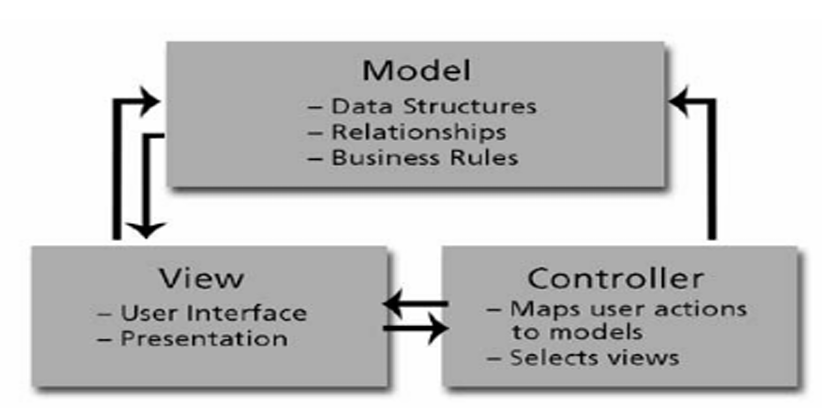
\includegraphics[width=0.5\textwidth]{images/MVC_architecture.png}
		\caption{zeigt die Model-View-Controller (MVC)-Architektur, die eine klare Trennung zwischen Daten, Benutzeroberfläche und Logik bietet. \textit{\cite{madurapperuma2022state}}}
	\end{figure}
	
	\item Sie bieten standardisierte Funktionen wie Datenbindung (z. B. in Angular oder Vue.js), virtuelle DOM-Verarbeitung (z. B. in React) und Werkzeuge für die Performance-Optimierung.\textit{\cite{awasthiresearch}}
\end{itemize}

\subsubsection{Vorteile von Webframeworks}
\begin{itemize}
	\item \textbf{Beschleunigte Entwicklung}: Frameworks wie Angular, React oder Vue.js bieten Module und Werkzeuge, die Entwicklern ermöglichen, weniger Code zu schreiben und gleichzeitig hohe Qualität zu gewährleisten.\textit{\cite{hutagikar2020analysis}}
	
	
	\item \textbf{Flexibilität und Performance}: Technologien wie Reacts virtueller DOM oder Vue.js’ modulare Architektur ermöglichen die Erstellung dynamischer und leistungsfähiger Anwendungen.\textit{\cite{shetty2020review}}
	
	\item \textbf{Skalierbarkeit}: Backend-Frameworks wie Node.js und Frontend-Frameworks wie Angular sind speziell auf wachsende Anforderungen optimiert und unterstützen einfache Erweiterungen.\textit{\cite{madurapperuma2022state}}
	
\end{itemize}

\subsubsection{Nachteile von Webframeworks}
\begin{itemize}
	\item \textbf{Lernkurve}: Frameworks wie Angular führen zusätzliche Konzepte wie TypeScript ein, die eine längere Einarbeitungszeit erfordern. Andere wie React erfordern das Verständnis von JSX und State Management.\textit{\cite{awasthiresearch, rathinam2022analysis}}
	
	
	\item \textbf{Abhängigkeit von der Auswahl}: Die Wahl eines falschen Frameworks kann zu Schwierigkeiten in der Entwicklung und Performance-Problemen führen. Zum Beispiel ist Angular ideal für große Anwendungen, während Vue.js besser für kleinere Projekte geeignet ist.\textit{\cite{rathinam2022analysis}}
	
\end{itemize}

\begin{figure}
	\centering
	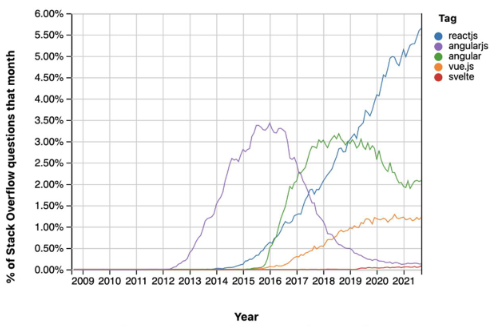
\includegraphics[width=0.5\textwidth]{images/framework_popularity.png}
	\caption{zeigt die Popularität verschiedener Frontend-Frameworks über die Jahre, basierend auf dem Anteil der Fragen auf Stack Overflow. \textit{\cite{akivab_js_framework}}}
\end{figure}



\subsubsection{Angular}

\textbf{Einführung in Angular}
\newline
Angular ist ein quelloffenes Framework für die Frontend-Webentwicklung, das von Google entwickelt wurde. Es wurde erstmals 2010 als AngularJS eingeführt und mit Angular 2 vollständig überarbeitet. Es basiert auf TypeScript und ermöglicht die Erstellung dynamischer, skalierbarer Single-Page-Anwendungen (SPAs). Durch regelmäßige Updates bleibt Angular ein modernes Framework, das an die Anforderungen der Webentwicklung angepasst ist.\textit{\cite{madurapperuma2022state, shetty2020review, angular}} \newline


\textbf{Architektur}
\newline
Angular verwendet eine komponentenbasierte Architektur, bei der die Benutzeroberfläche in kleine, wiederverwendbare Teile (Komponenten) unterteilt wird. Jede Komponente besteht aus:

\begin{itemize}
	\item \textbf{Templates}: HTML, erweitert mit Angular-spezifischen Direktiven.
	\item \textbf{Styles}: CSS oder SCSS für das Design.
	\item \textbf{Logik}: TypeScript für die Geschäftslogik.
\end{itemize}

Komponenten werden in Modulen (\texttt{NgModules}) gruppiert, um eine bessere Organisation und Wiederverwendbarkeit zu gewährleisten. Diese Struktur fördert die Modularität und erleichtert die Wartung des Codes.\textit{\cite{hutagikar2020analysis, shetty2020review, angular}} \newline

\textbf{Hauptfunktionen von Angular}

\textbf{Datenbindung} 

Angular unterstützt sowohl Einweg- als auch Zweiweg-Datenbindung:

\begin{itemize}
	\item \textbf{Einweg-Datenbindung}: Daten fließen nur vom Model zur View.
	\item \textbf{Zweiweg-Datenbindung}: Änderungen in der View werden automatisch an das Model zurückgegeben und umgekehrt. Dies wird häufig für Formulare verwendet und reduziert den manuellen Aufwand bei der Synchronisation.\textit{\cite{hutagikar2020analysis, madurapperuma2022state, angular}}
\end{itemize}

\textbf{Vorteile von Angular}
\begin{itemize}
	\item \textbf{Skalierbarkeit}: Angular eignet sich sowohl für kleine als auch für große Projekte, dank seiner Modularität und TypeScript-Unterstützung.\textit{\cite{madurapperuma2022state, rathinam2022analysis, angular}}
	
	\item \textbf{Integrierte Tools}: Angular CLI (Command Line Interface) erleichtert die Projektinitialisierung, den Build-Prozess und das Testen. Angular Material bietet vorgefertigte UI-Komponenten, die das Design beschleunigen.\textit{\cite{hutagikar2020analysis, angular_blog}}
	
	\item \textbf{Community und Support}: Als von Google unterstütztes Framework verfügt Angular über eine aktive Entwicklergemeinschaft, regelmäßige Updates und umfassende Dokumentation.\textit{\cite{shetty2020review, angular}}
\end{itemize}

\textbf{Nachteile von Angular}
\begin{itemize}
	\item \textbf{Steile Lernkurve}: Durch die Einführung von TypeScript, Dependency Injection und einer komplexen Struktur ist Angular für Anfänger herausfordernd.\textit{\cite{madurapperuma2022state, rathinam2022analysis, angular_blog}}
	\item \textbf{Framework-Größe}: Angular ist im Vergleich zu leichtgewichtigen Frameworks wie Vue.js oft schwerer und kann dadurch die Ladezeit beeinflussen.\textit{\cite{shetty2020review, angular}}
\end{itemize}


\subsubsection{React}

\textbf{Einführung in React}
\newline
React ist eine quelloffene JavaScript-Bibliothek, die von Meta (ehemals Facebook) entwickelt wurde und hauptsächlich zur Erstellung von Benutzeroberflächen verwendet wird. Sie wurde erstmals 2013 veröffentlicht und ist besonders für die Entwicklung dynamischer Single-Page-Anwendungen (SPAs) geeignet. React basiert auf dem Konzept von Komponenten und der Verwendung eines virtuellen DOM, um die Performance zu optimieren. Es bietet eine flexible Architektur für die Entwicklung moderner Webanwendungen.\textit{\cite{rathinam2022analysis, hutagikar2020analysis, react}} \newline

\textbf{Architektur}
\newline
React verwendet eine komponentenbasierte Architektur, bei der Benutzeroberflächen in kleinere, wiederverwendbare Teile aufgeteilt werden. Diese Architektur ermöglicht eine einfache Wartung und Erweiterung von Anwendungen. Jede Komponente in React ist in JSX (JavaScript XML) geschrieben, einer Syntaxerweiterung, die HTML-ähnlichen Code innerhalb von JavaScript erlaubt.

\begin{itemize}
	\item \textbf{Virtueller DOM}: React verwendet einen virtuellen DOM, der Änderungen an der Benutzeroberfläche effizient berechnet und nur die betroffenen Teile des echten DOM aktualisiert.
	\item \textbf{JSX}: JSX ist eine Mischung aus JavaScript und HTML, die es Entwicklern ermöglicht, benutzerdefinierte UI-Komponenten zu erstellen.
	\item \textbf{Unidirektionaler Datenfluss}: Daten fließen in React in einer einzigen Richtung, was die Verwaltung und Nachverfolgbarkeit von Daten einfacher macht.\textit{\cite{rathinam2022analysis, hutagikar2020analysis, react}}
\end{itemize}

\textbf{Hauptfunktionen von React}

\textbf{Komponentenbasierte Entwicklung} 

React ermöglicht die Erstellung von wiederverwendbaren und modularen Komponenten, die sowohl die Benutzeroberfläche als auch die Logik kapseln. Dies fördert eine bessere Strukturierung und Wartbarkeit des Codes.\textit{\cite{shetty2020review, react}}

\textbf{Virtueller DOM} 

Der virtuelle DOM verbessert die Performance von React-Anwendungen, indem er Änderungen effizient berechnet und nur die betroffenen Teile des echten DOM aktualisiert. Dies reduziert die Anzahl der direkten DOM-Manipulationen erheblich.\textit{\cite{rathinam2022analysis, hutagikar2020analysis, react}}

\textbf{Vorteile von React}
\begin{itemize}
	\item \textbf{Performance}: Der virtuelle DOM und die asynchrone Verarbeitung ermöglichen eine schnelle und effiziente Benutzeroberfläche.\textit{\cite{rathinam2022analysis, react}}
	
	\item \textbf{Flexibilität und Wiederverwendbarkeit}: Die komponentenbasierte Architektur von React erleichtert die Wiederverwendung von Code und die Skalierung von Anwendungen.\textit{\cite{hutagikar2020analysis, react}}
	
	\item \textbf{Große Community und Ökosystem}: React wird von einer riesigen Entwicklergemeinschaft unterstützt, und es gibt zahlreiche Bibliotheken und Tools, die den Entwicklungsprozess verbessern.\textit{\cite{shetty2020review, react}}
\end{itemize}

\textbf{Nachteile von React}
\begin{itemize}
	\item \textbf{Zusätzliche Abhängigkeiten}: React bietet nur die grundlegende Architektur, weshalb oft zusätzliche Bibliotheken (z. B. für Routing oder State Management) benötigt werden.\textit{\cite{shetty2020review, rathinam2022analysis, react_blog}}
	
	\item \textbf{Lernkurve}: Für Entwickler, die mit JSX und der Unidirektionalität des Datenflusses nicht vertraut sind, kann React eine gewisse Lernkurve darstellen.\textit{\cite{hutagikar2020analysis, react_blog}}
\end{itemize}



\subsubsection{Vue.js}

\textbf{Einführung in Vue.js}
\newline
Vue.js ist ein progressives JavaScript-Framework, das 2014 von Evan You entwickelt wurde. Es wird häufig für die Erstellung von Benutzeroberflächen und Single-Page-Anwendungen (SPAs) verwendet. Vue.js zeichnet sich durch seine einfache Integration in bestehende Projekte und seine Flexibilität aus, wodurch es sowohl für kleine als auch große Anwendungen geeignet ist. Durch seine modulare Struktur und starke Community-Unterstützung bleibt Vue.js ein beliebtes Framework für Webentwickler.\textit{\cite{rathinam2022analysis, madurapperuma2022state, vuejs}} \newline

\textbf{Architektur}
\newline
Vue.js verwendet die Model-View-ViewModel (MVVM)-Architektur, die es ermöglicht, die Benutzeroberfläche, die Geschäftslogik und die Datenbindung effizient zu verwalten. Die Hauptbestandteile von Vue.js sind:

\begin{itemize}
	\item \textbf{Templates}: Vue.js verwendet Templates, um UI-Komponenten zu definieren. Diese Templates werden in renderbare DOM-Elemente übersetzt.
	\item \textbf{Reaktivitätssystem}: Das reaktive Datenmodell von Vue.js ermöglicht automatische Updates der Benutzeroberfläche, wenn sich die zugrunde liegenden Daten ändern.
	\item \textbf{Direktiven}: Vue.js bietet spezielle HTML-Attribute (Direktiven), die Funktionen wie Schleifen, Bedingungen und Ereignishandlungen erleichtern.\textit{\cite{hutagikar2020analysis, vuejs}}
\end{itemize}

\textbf{Hauptfunktionen von Vue.js}

\textbf{Komponentenbasierte Entwicklung} 

Wie React und Angular ermöglicht Vue.js die Erstellung von wiederverwendbaren und modularen Komponenten. Diese Struktur fördert die Organisation und erleichtert die Wartung und Erweiterung von Anwendungen.\textit{\cite{rathinam2022analysis, vuejs}}

\textbf{Reaktivitätssystem} 

Das Reaktivitätssystem von Vue.js überwacht automatisch Änderungen im Datenmodell und aktualisiert die Benutzeroberfläche entsprechend. Dies macht die manuelle DOM-Manipulation überflüssig und verbessert die Entwicklererfahrung.\textit{\cite{hutagikar2020analysis, vue_blog}}

\textbf{Vorteile von Vue.js}
\begin{itemize}
	\item \textbf{Einfache Lernkurve}: Vue.js ist einfach zu lernen, da es eine klare und intuitive Syntax bietet. Es ist besonders für Entwickler geeignet, die mit HTML, CSS und JavaScript vertraut sind.\textit{\cite{madurapperuma2022state, vuejs}}
	
	\item \textbf{Flexibilität und Modularität}: Vue.js kann sowohl für einfache Widgets als auch für komplexe Anwendungen verwendet werden. Seine modulare Struktur ermöglicht eine einfache Integration in bestehende Projekte.\textit{\cite{rathinam2022analysis, vuejs}}
	
	\item \textbf{Leichtgewichtig und performant}: Vue.js ist kleiner als Frameworks wie Angular und React, was die Ladezeit reduziert und die Performance verbessert.\textit{\cite{shetty2020review, vuejs}}
\end{itemize}

\textbf{Nachteile von Vue.js}
\begin{itemize}
	\item \textbf{Geringere Unterstützung durch große Unternehmen}: Im Gegensatz zu React und Angular wird Vue.js nicht von einer großen Organisation unterstützt, was in einigen Fällen zu Unsicherheiten führen kann.\textit{\cite{rathinam2022analysis, vue_blog}}
	
	\item \textbf{Weniger umfangreiches Ökosystem}: Während Vue.js eine starke Community hat, sind bestimmte Drittanbieter-Bibliotheken und Tools im Vergleich zu React und Angular weniger verbreitet.\textit{\cite{hutagikar2020analysis, vue_blog}}
\end{itemize}


% Dokumente für State of the Art

\chapter{State of the art}

\setauthor{Manuel Fellner}
\section{Vorhandene Backend-Technologien}

Für das Projekt stehen die folgenden populären Technologien zur Verfügung: \textbf{Django}, \textbf{Flask}, \textbf{ExpressJS} und \textbf{Spring Boot}. Diese bilden die Grundpfeiler der Entwicklung weltweit und werden von unzähligen Organisationen aktiv verwendet und empfohlen, wie unter \cite{website-popular-backend-framework} ersichtlich ist. Siehe Prompt \cite{prompt-gpt-list-to-text-individual}.

\subsection{Django}
Django ist ein \gls{full-stack-framework}, das durch seinen umfassenden Funktionsumfang zahlreiche Anwendungsfälle abdeckt. Eine gute Übersicht darüber lässt sich unter \cite{website-django-functionality-summary} finden. Die Implementierung gestaltet sich relativ einfach, da zahlreiche Anleitungen und Ressourcen im Internet verfügbar sind. Allerdings weist Django einen erhöhten Arbeitsaufwand beim Erlernen auf, was insbesondere bei Einsteigern einen erhöhten Einarbeitungsaufwand erfordert.

Das Projektteam verfügt über solide Kenntnisse in der Programmiersprache Python, wodurch die Nutzung des Frameworks erleichtert wird. Hinsichtlich der Skalierbarkeit bietet Django viele Optionen, jedoch stellt die monolithische Architektur des Frameworks eine gewisse Einschränkung dar. Skalierungsmaßnahmen erfordern in der Regel Anpassungen am gesamten Projekt, was zeitaufwendig sein kann.

Ein großer Vorteil von Django liegt im Bereich der Sicherheit (siehe \cite{website-django-security-summary}). Das Framework enthält bereits integrierte Schutzmaßnahmen gegen gängige Web-Angriffe wie \gls{sql-injection} und \gls{xss-attack}. Darüber hinaus bietet es unter anderem Funktionen wie Passwort-Hashing und vorgefertigte Bibliotheken für die Authentifizierung und Autorisierung an.

In Bezug auf die Performance verfügt Django über eine automatische \gls{caching}-Funktion \cite{website-django-caching}, die eine effiziente Verarbeitung von Hintergrundprozessen ermöglicht. Allerdings bringt der große Funktionsumfang eine höhere Ressourcenbelastung mit sich. 

Die Community rund um Django ist äußerst aktiv. Auf \cite{website-stackoverflow-django} gibt es über 312.000 beantwortete Fragen zu diesem Framework, was die Qualität des Community-Supports unterstreicht. Zudem ist die offizielle Dokumentation von Django umfangreich und gut strukturiert, was die Einarbeitung erleichtert. \cite{website-django-docs}

Ein weiterer Vorteil von Django ist die einfache Integration als reines Backend über das \textit{Django REST Framework}, siehe \cite{website-django-rest-framework}. Das Framework unterstützt nahezu alle relationalen Datenbanken, was es vielseitig einsetzbar macht.


\subsection{Flask}
Flask ist ein leichtgewichtiges Micro-Framework, das sich durch seine kompakte Größe und hohe Flexibilität auszeichnet, was \cite{website-flask-overview} noch einmal unterstreicht. Die Implementierung gestaltet sich sehr einfach, da das Framework nur wenige Abhängigkeiten mitbringt und eine minimale Grundstruktur erfordert. Dies erleichtert den Einstieg in die Entwicklung. Das von Flask selbst bereitgestellte Tutorial (siehe \cite{website-flask-tutorial}) bietet einen guten Überblick über diesen schnellen Einstieg. 

Wie bei Django basiert Flask auf der Programmiersprache Python, was für das Projektteam von Vorteil ist. Die Nutzung bekannter Sprachstrukturen führt zu einer schnellen und effizienten Entwicklung.

Flask unterstützt eine Microservice-Architektur, die eine flexible Skalierbarkeit ermöglicht. Einzelne Dienste können unabhängig voneinander erstellt und erweitert werden. Allerdings bringt die geringe Anzahl integrierter Funktionen auch Herausforderungen mit sich: Für größere Projekte ist Flask weniger geeignet, da viele Funktionen manuell ergänzt werden müssen.

Hinsichtlich der Sicherheit bietet Flask grundlegende Mechanismen, jedoch müssen diese größtenteils vom Entwickler konfiguriert werden. Dies erhöht den Aufwand für die Absicherung der Anwendung. Eine Bibliothek, welche von einem Drittanbieter zur Verfügung gestellt wird, wäre zum Beispiel Flask Security (sieh \cite{website-flask-security}).

Flask überzeugt mit seiner Performance. Aufgrund der kompakten Struktur und der einfachen Architektur ist das Framework äußerst ressourcenschonend und performant.

Die Community von Flask ist ebenfalls groß, allerdings wird kein offizieller Hersteller-Support angeboten. Auf Stackoverflow, siehe \cite{website-stackoverflow-flask}, sind über 55.000 Fragen zum Framework beantwortet worden, was die Verfügbarkeit von Community-Ressourcen bestätigt.

In Bezug auf die Dokumentation ist Flask zwar gut dokumentiert, jedoch weniger umfassend als andere Frameworks wie Django. Die Integration mit dem Frontend erfolgt meist über den \textit{API-First-Ansatz}, bei dem spezifische API-Endpunkte definiert werden. Dies bietet eine hohe Flexibilität bei der Anbindung von relationalen Datenbanken.


\subsection{ExpressJS}
ExpressJS ist ein Backend-Framework, das auf Node.js basiert und sich durch seine Einfachheit und Flexibilität auszeichnet (siehe \cite{website-expressjs}). Die Implementierung erfolgt weitgehend unkompliziert, erfordert jedoch an einigen Stellen manuelle Konfigurationen, um bestimmte Funktionen zu aktivieren.

Die Programmiersprache von ExpressJS ist JavaScript, welches vom gesamten Projektteam beherrscht wird. Allerdings sind spezifische Kenntnisse in Node.js noch nicht umfassend vorhanden. Dennoch erleichtert die Vertrautheit mit JavaScript den Einstieg in die Entwicklung.

In Bezug auf die Skalierbarkeit bietet ExpressJS viele Optionen, wie in \cite{website-express-scaling} beschrieben wird. Die Nutzung von externen Bibliotheken sowie die Unterstützung von asynchronen Prozessen ermöglicht es, Anwendungen flexibel zu erweitern. Diese Skalierbarkeit ist besonders wichtig für größere Anwendungen.

Die Sicherheit in ExpressJS hängt stark von den implementierten Sicherheitsmaßnahmen des Entwicklers ab. Zwar gibt es viele verfügbare Bibliotheken für die Absicherung, jedoch sind diese nicht von Haus aus in das Framework integriert. Eine Übersicht der verfügbaren Maßnahmen findet man unter \cite{website-express-security}.

Ein großer Vorteil von ExpressJS ist die Performance. Dank der asynchronen Prozessverarbeitung von Node.js werden Anfragen nicht sequenziell, sondern parallel bearbeitet. Dies führt zu einer erheblichen Beschleunigung der Verarbeitungsgeschwindigkeit.

Die Community rund um ExpressJS ist sehr aktiv. Auf Stackoverflow wurden über 95.000 Fragen zu dem Framework beantwortet, siehe \cite{website-stackoverflow-expressjs}. Die offizielle Dokumentation ist zwar vorhanden, aber oft nicht ausreichend, um komplexe Anwendungen ohne zusätzliche Quellen von Drittanbietern zu entwickeln.

Die Integration mit dem Frontend erfolgt über die Erstellung von REST-APIs, was den Datenaustausch zwischen Frontend und Backend vereinfacht.


\subsection{Spring Boot}
Spring Boot ist ein modernes Framework, das auf der Programmiersprache Java basiert und durch seine Service-orientierte Architektur überzeugt. \cite{website-springboot} Die Implementierung gestaltet sich besonders einfach, da Spring Boot zahlreiche Funktionen bereitstellt. Mithilfe des \textit{Spring Initializr} \cite{website-spring-initializr} können Projektstrukturen automatisch generiert werden, was den Einstieg erheblich erleichtert.

Das Projektteam verfügt über fundierte Kenntnisse in Java, da diese Programmiersprache im Unterricht umfassend behandelt wurde. Dadurch lässt sich Spring Boot effizient nutzen.

Die Skalierbarkeit von Spring Boot ist hervorragend. \cite{website-spring-scaling} Aufgrund der service-orientierten Architektur können einzelne Services unabhängig voneinander erstellt und erweitert werden. Dies ähnelt der Microservice-Architektur und ermöglicht es, komplexe Anwendungen modular zu gestalten.

Spring Boot überzeugt im Bereich der Sicherheit durch die Erweiterung \textit{Spring Security} \cite{website-spring_security}, die Authentifizierungs- und Autorisierungsfunktionen integriert. Diese Sicherheitsmaßnahmen entsprechen aktuellen Industriestandards. \cite{website-security-industry-standards}

In Bezug auf die Performance bietet Spring Boot solide Ergebnisse. Die service-orientierte Architektur in Kombination mit Java als Programmiersprache sorgt, im Vergleich zu Django, für eine hohe Verarbeitungsgeschwindigkeit und Stabilität (siehe \cite{website-performance-spring-boot-vs-django}).

Die Community von Spring Boot ist groß und aktiv. Laut \cite{website-stackoverflow-spring-boot} sind über 212.000 Fragen zu dem Framework beantwortet worden, was auf eine starke Unterstützung durch die Community hinweist.

Schließlich überzeugt Spring Boot mit einer umfangreichen und übersichtlichen Dokumentation, die Entwicklern eine klare Orientierung bietet. \cite{website-spring-docs} Die Integration mit anderen Technologien ist durch die modulare Struktur des Frameworks einfach möglich, was die Anbindung an Frontend-Systeme und Datenbanken erleichtert. 

\newpage



\setauthor{Sebastian Sailer}
\section{Datenbankmanagementsysteme}
Datenbanken haben seit ihrer Entstehung eine signifikante Entwicklung durchlaufen. Ziel der State-of-the-Art-Analyse ist es, derzeit relevante Datenbankmanagementsysteme systematisch zu untersuchen und vorzustellen.

\vspace{5mm}\makefig{images/statistikDBMS.png}{height=10cm}{ Beliebtesten Datenbankmanagementsysteme weltweit laut Statista \cite{Statista:DBMS}}{fig:caption-label}

\noindent Die im Juni 2024 veröffentlichte, oben dargestellte Grafik (Abbildung 5.1), zeigt die Verteilung der Beliebtheit von Datenbankmanagementsystemen anhand einiger verschiedener Kriterien. \newline Dazu zählen die Anzahl der Erwähnungen in Suchmaschinenergebnissen, das allgemeine Interesse laut Google Trends, die Häufigkeit technischer Diskussionen auf Plattformen wie Stack Overflow, die Nennung in Jobangeboten, die Präsenz in LinkedIn-Profilen sowie die Relevanz in sozialen Netzwerken wie X (ehemals Twitter). Aus dem Zusammenspiel all dieser Kriterien entstand die auf Statista veröffentlichte und von Petroc Taylor erstellte Grafik.

\newpage
\subsection{Beliebteste DBMS}
Da eine Analyse aller in Abbildung 3 dargestellten DBMS den Rahmen  sprengen würde, schließen wir einige Systeme wie \textbf{Microsoft SQL Server} oder \textbf{Oracle Database} aus. Das Ausschlusskriterium bei diesen DBMS ist der finanzielle Aspekt.

\vspace{2mm} \noindent Microsoft Access kommt ebenso nicht infrage, da es zwar für kleine Anwendungen mit wenigen Benutzern und geringen Datenmengen sinnvoll ist, jedoch zum Speichern und effizienten Verwalten von größeren Datenmengen nicht geeignet ist. Microsoft Access ist aufgrund von Skalierungs-, Performance- und Mehrbenutzerproblemen keine geeignete Wahl für dieses Projekt, siehe \cite{MSAccess:Comparison}.

\vspace{2mm}
\noindent In diesem Projekt liegt das Hauptaugenmerk auf hoher Performance und Skalierbarkeit, um eine zukunftssichere Erweiterbarkeit zu gewährleisten. (Prompt: \cite{ChatGPT:rewrite1})

\vspace{3mm} 
\noindent Aufgrund dessen erfolgt eine Vorstellung der folgenden vier Datenbankmanagementsysteme, gefolgt von einem Vergleich ihrer Vor- und Nachteile: \textbf{PostgreSQL}, \textbf{MariaDB}, \textbf{Amazon Aurora} und \textbf{MongoDB}.


\subsubsection{PostgreSQL}
PostgreSQL ist ein \gls{ac-ORDB}, welches, laut \cite{PostgreSQL:Hersteller}, ursprünglich aus dem von der University of California at Berkeley entwickelten POSTGRES 4.2 hervorgegangen ist. Es zeichnet sich durch Stabilität, Erweiterbarkeit und Unterstützung komplexer Datentypen aus, wie \cite{PostgreSQL:IBM} beschreibt. Als modernes \gls{Open-Source}-DBMS ist es ACID-konform, kombiniert \textbf{relationale} und \textbf{objektorientierte} Modelle und bietet Hochverfügbarkeit. Dank effizienter Skalierbarkeit und paralleler Abfragen eignet sich PostgreSQL für vielfältige Anwendungen, von Webanwendungen bis hin zu Data-Warehousing. PostgreSQL wird kontinuierlich weiterentwickelt und kann ohne \gls{Kosten} für jegliche Zwecke verwendet werden. \cite{PostgreSQL:Usage} beschreibt bekannte Projekte, welche PostgreSQL zur Realisierung benutzen, sind \textbf{Amazon Web Services} und \textbf{AIVEN}. 


\subsubsection{MariaDB}
MariaDB ist ebenso ein leistungsstarkes, vollständig Open-Source-basiertes relationales Datenbankmanagementsystem, das aus einem \gls{Fork} von MySQL hervorgegangen ist. Es wurde entwickelt, um MySQL zu ersetzen und bietet zusätzliche Funktionen wie erweiterte Performance und optimierte Replikation, wie in Pierre Mavro's Buch \cite{Buch:PierreMavro} genauer erläutert wird . MariaDB unterstützt moderne Anforderungen wie hohe Skalierbarkeit und \gls{Datenbank-Sharding} und wird von einer aktiven Community weiterentwickelt und betreut, sowie von großen Unternehmen wie Wikipedia, WordPress und Google genutzt. \cite{MariaDB:Intro} behauptet, dass MariaDB besonders für performante und skalierbare Anwendungen geeignet ist. 



\newpage
\subsubsection{MongoDB}
MongoDB ist ein flexibles, dokumentenbasiertes NoSQL-Datenbankmanagementsystem, welches sich laut \cite{MongoDB:Introduction} durch horizontale Skalierbarkeit, hohe Agilität und flexible Datenmodellierung auszeichnet. Es wird oft für moderne Anwendungen verwendet, da das Speichern von Daten in \gls{ac-JSON}-ähnlichen Dokumenten geschieht. Der Hersteller gibt an hier \cite{MongoDB:Databases} an, dass MongoDB sowohl selbstverwaltete als auch vollständig cloudbasierte Lösungen bietet. (z.B.: MongoDB Atlas, eine Plattform, die in über 100 Regionen auf AWS, Google Cloud und Azure verfügbar ist). MongoDB wird außerdem von einigen großen Dienstleistern wie unter anderem \textbf{accenture}, \textbf{cisco} und \textbf{Toyota connected} verwendet. \cite{MongoDB:MainPage}\newline 


\begin{lstlisting}[language=Java, caption={Beispiel für ein JSON-Objekt, welches in einer MongoDB Datenbank gespeichert sein könnte \cite{MongoDB:JSON}}]
{
  "_id": 1,
  "name": {
    "first": "John",
    "last": "Backus"
  },
  "contribs": [
    "Fortran",
    "ALGOL",
    "Backus-Naur Form",
    "FP"
  ],
  "awards": [
    {
      "award": "W.W. McDowell Award",
      "year": 1967,
      "by": "IEEE Computer Society"
    },
    {
      "award": "Draper Prize",
      "year": 1993,
      "by": "National Academy of Engineering"
    }
  ]
}    
\end{lstlisting}



\subsubsection{Amazon Aurora}
Amazon Aurora ist ein hochperformantes, vollständig verwaltetes relationales Datenbankmanagementsystem (RDBMS), welches von \gls{Amazon Web Services} entwickelt wurde. Es kombiniert die Skalierbarkeit von Open-Source-Datenbanken mit der Leistung kommerzieller und ist dabei, laut eigenen angeben, Kosteneffizient. Ebenso gibt Amazon an \cite{Amazon:S3}, erweiterte Funktionen wie automatische Skalierung und kontinuierliche Sicherung in \gls{Amazon S3} anzubieten. Es unterstützt sowohl MySQL- als auch PostgreSQL-Kompatibilität, wodurch eine problemlose Migration in bestehende Anwendungen ermöglicht wird. Mit einer Verfügbarkeit von bis zu "99,99\% " \textit{-AWS \cite{Amazon:aurora}} und einer hohen Ausfallsicherheit ist es ideal für moderne Anwendungen, die hohe Leistung, Skalierbarkeit und Zuverlässigkeit erfordern. Laut \cite{Amazon:aurora} nutzen große Firmen wie Samsung, Panasonic und Nintendo nutzen die Dienste von Amazon Aurora. 


\setauthor{Sebastian Pollak}

\section{Formularsysteme}

    Im folgenden Teil wird eine umfassende Analyse der derzeit führenden Methoden zur Implementierung von Formularen und Formularvalidierung durchgeführt. Dies zielt darauf ab, einen detaillierten Überblick über die aktuellen Best Practices und technologischen Ansätze zu bekommen.\cite{prompt10_pollak}

    \subsection{Wichtige Konzepte in \gls{react}}
    Bevor wir in die spezifischen Frameworks und Bibliotheken eintauchen, ist es wichtig, einige grundlegende Konzepte der Formularerstellung in React zu verstehen. Diese Konzepte bilden die Grundlage für viele der vorgestellten Frameworks und deren Architektur.
    
        \subsubsection{React Hooks\label{sec:ReactHooks}}
        Wie in der React-Dokumentation \cite{reacthooks} nachzulesen, sind React Hooks Funktionen, mit denen React-Features direkt in den Komponenten genutzt werden können. Sie erlauben es zum Beispiel, State und andere React-Features zu verwenden, ohne eine Klasse schreiben zu müssen. Ein State-Hook könnte beispielsweise folgendermaßen aussehen:
    
        \begin{lstlisting}[language=JavaScript]
    function Counter() { 
        const [count, setCount] = useState(0); 
        return (
            <div>
                <p>Count: {count}</p> 
                <button onClick={() => setCount(count + 1)}>Increment</button>  
            </div>
        );
    }
        \end{lstlisting}
        In diesem Beispiel wird count durch den ''useState''-Hook verwaltet und durch die ''setCount''-Funktion aktualisiert.

        \subsubsection{Controlled und Uncontrolled Komponenten}
        Bei der Arbeit mit Formularen in \gls{react} gibt es zwei grundlegende Arten von Komponenten: Controlled- und Uncontrolled-Komponenten.
        
        \paragraph{Controlled Komponenten}
        Wie man in der React-Dokumentation \cite{react_forms} nachlesen kann, wird der Zustand bei Controlled Komponenten durch den React State verwaltet. Das bedeutet, dass jedes Eingabefeld seinen Wert aus dem State bezieht und jede Änderung des Werts den State aktualisiert. Controlled Komponenten bieten somit die vollständige Kontrolle über das Formular und die Eingabewerte.
        
        Abbildung \ref{fig:controlled-component} veranschaulicht den Datenfluss einer Controlled-Komponente. Jede Benutzereingabe löst ein Event aus, das vom Event-Handler verarbeitet wird, welcher wiederum den State aktualisiert. Der State gibt den neuen Wert an das Eingabefeld zurück, wodurch der Datenfluss vollständig kontrolliert wird.
        
        \begin{figure}[H]
            \centering
            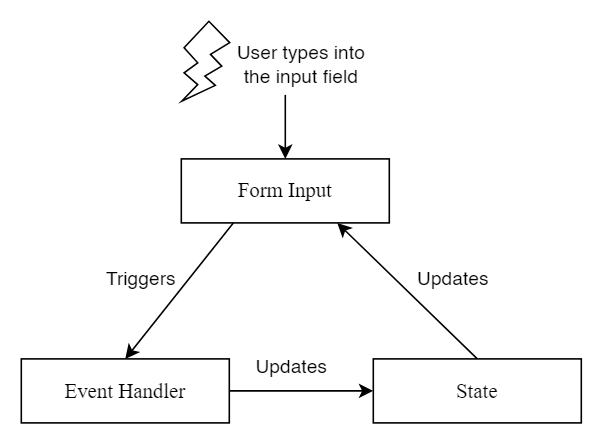
\includegraphics[width=0.7\linewidth]{images/controlledComponent.png}
            \caption{Datenfluss in Controlled Komponenten, Quelle: \cite{controlled_inputs_diagram}}
            \label{fig:controlled-component}
        \end{figure}

        Ein Beispiel für die Initialisierung des States und das Handling von Änderungen sieht wie folgt aus:
        
        \begin{lstlisting}[language=JavaScript]
        const [name, setName] = useState(""); 
        
        const handleChange = (e) => {
            setName(e.target.value); 
        };
        \end{lstlisting}
        
        In diesem Code wird der State für das Eingabefeld ''name'' initialisiert und mit der Funktion ''handleChange'' aktualisiert, sobald der Benutzer eine Eingabe tätigt. Jede Änderung des Eingabefelds löst ein Event aus, das vom Event-Handler verarbeitet wird, um den neuen Wert im State zu speichern.
        
        Die Verbindung zwischen dem State und dem Eingabefeld wird durch die Verwendung des Attributs ''value'' hergestellt.
        
        \begin{lstlisting}[language=JavaScript]
        return (
            <form onSubmit={handleSubmit}> 
                <input type="text" value={name} onChange={handleChange} />  
                <button type="submit">Submit</button> 
            </form>
        );
        \end{lstlisting}

        In diesem Beispiel wird der Wert des Eingabefeldes ''name'' durch den State gesteuert, und jede Änderung wird durch die Funktion ''handleChange'' verarbeitet.
        
        \paragraph{Uncontrolled Komponenten\label{sec:uncontrolledComponents}}
        Im Gegensatz zu Controlled Komponenten, wie in \cite{react_uncontrolled_components} beschrieben, wird bei Uncontrolled Komponenten der Zustand des Eingabefeldes nicht durch den React State, sondern direkt durch das DOM verwaltet. Dies bedeutet, dass der Wert eines Eingabefeldes über ein ''ref''-Objekt zugänglich ist, wodurch eine direkte Interaktion mit dem DOM ermöglicht wird.
        
        Ein Beispiel für die Initialisierung eines ''ref''-Objekts und dessen Verwendung sieht wie folgt aus:
        
        \begin{lstlisting}[language=JavaScript]
        const inputRef = useRef(); 
        
        const handleSubmit = (e) => {
            console.log(inputRef.current.value);  
        };
        \end{lstlisting}
        
        In diesem Code wird das ''ref''-Objekt durch die Funktion ''useRef'' initialisiert. Dieses Objekt ermöglicht den Zugriff auf das DOM-Element des Eingabefeldes. Die Funktion `handleSubmit` zeigt, wie der aktuelle Wert des Eingabefeldes über das ''ref''-Objekt abgerufen werden kann. Dies unterscheidet sich grundlegend von Controlled-Komponenten, bei denen der Wert im React-State gespeichert wird.
        
        Die vollständige Implementierung einer Uncontrolled-Komponente könnte wie folgt aussehen:
        
        \begin{lstlisting}[language=JavaScript]
        return (
            <form onSubmit={handleSubmit}> 
                <input type="text" ref={inputRef} />  
                <button type="submit">Submit</button>  
            </form>
        );
        \end{lstlisting}
        
        In diesem Beispiel verwenden wir ''useRef'' zur direkten Referenzierung des DOM-Elements und zum Abrufen des Werts, ohne den State von \gls{react} zu nutzen.
        
    \subsection{React Hook Form}
        \subsubsection{Funktionsweise und Architektur} 
        Wie in \cite{reacthookform} ausführlich beschrieben, ist React Hook Form ein leichtgewichtiges Framework, welches das einfache Implementieren von Formularen mit integrierter Validierung in \gls{react}-Anwendungen ermöglicht. Das Ziel dieses Frameworks ist die Optimierung der Benutzer- und Entwickler-Experience. Dies geschieht in erster Linie durch Performance-Optimierungen. Es basiert, wie der Name schon sagt, auf dem Prinzip der oben erklärten React Hooks \ref{sec:ReactHooks}. \cite{prompt12_pollak}

            \paragraph{Verwaltung von Formularzuständen}
            Das React Hook Form nutzt Uncontrolled Komponenten (siehe Abschnitt \ref{sec:uncontrolledComponents}), da der Formularzustand direkt im DOM verwaltet wird und nicht im React-State. Diese Architektur führt zu einer verbesserten Effizienz, da Re-Renders minimiert werden und die Performance dadurch gesteigert wird.

            \paragraph{Beispiel}
            Die Verwendung von React Hook Form beginnt mit der Initialisierung des Formulars und der Registrierung der Eingabefelder:
            
            \begin{lstlisting}[language=JavaScript]
            const { register, handleSubmit } = useForm(); 
            
            const onSubmit = (data) => {  
                console.log(data); 
            };
            \end{lstlisting}
            
            In diesem Codeblock wird das Formular initialisiert, indem der Hook ''useForm'' verwendet wird. Die Funktion ''register'' dient dazu, Eingabefelder mit dem Formular zu verbinden, während ''handleSubmit'' die Verarbeitung der Formulardaten beim Absenden übernimmt. Die Funktion ''onSubmit'' wird aufgerufen, um die eingegebenen Daten weiterzuverarbeiten.
            
            Im nächsten Schritt wird gezeigt, wie diese Funktionen in einem Formular integriert werden:
            
            \begin{lstlisting}[language=JavaScript]
        return (
            <form onSubmit={handleSubmit(onSubmit)}>  
                <input {...register("name")} placeholder="Name" />  
                <input {...register("age")} type="number" placeholder="Age" /> 
                <button type="submit">Submit</button>  
            </form>
        );
            \end{lstlisting}
            
            In diesem Beispiel werden zwei Eingabefelder (''name'' und ''age'') registriert. Durch die Verwendung des Spread-Operators (''...register'') werden die Felder direkt mit dem Formular verbunden. Beim Absenden des Formulars ruft der Button die Funktion ''handleSubmit'' auf, welche wiederum die Funktion ''onSubmit'' ausführt. Dies ermöglicht eine einfache Verwaltung und Verarbeitung der Formulardaten.

        \subsubsection{Performance \label{sec:perfomanceHookForm}}
        Wie oben schon erwähnt wurde, ist das Hauptziel dieses Frameworks die Optimierung der Performance. Dies geschieht durch das Minimieren der Re-Renders. 

        Re-Rendern ist der Prozess, bei dem Komponenten neu geladen werden müssen, um Änderungen im Zustand oder in den Properties widerzuspiegeln. Dies benötigt logischerweise Rechenleistung. Um dies zu optimieren, wird versucht, diese auf das Minimum zu reduzieren. Dafür sorgt im Wesentlichen folgende Strategie:\cite{prompt12_pollak}

            \paragraph{Isolierte Re-Renders und Subscriptions}
            Wenn ein Benutzer in ein Eingabefeld tippt, wird nur dieses spezifische Feld aktualisiert, ohne dass der gesamte Formularbaum neu gerendert wird. Isolierte Re-Renders konzentrieren sich darauf, den Bereich des Re-Renderings auf spezifische Teile einer Komponente zu beschränken. Subscriptions hingegen überwachen Änderungen bestimmter Werte und lösen Re-Renders nur für die betroffenen Komponenten aus. Jedoch ist anzumerken, dass Formik im Vergleich zu React Hook Form tendenziell mehr Re-Renders verursachen kann, insbesondere bei großen Formularen. \cite{prompt13_pollak} \cite{prompt14_pollak}
                
        \subsubsection{Integration anderer Validierungsbibliotheken}
        \label{sec:IntegrationReactHookForm}
        React Hook Form ermöglicht es auch, Validierungsschemata anderer Validierungsbibliotheken zu verwenden. Es können Yup, Zod, Superstruct und Joi verwendet werden. Dabei übernimmt die externe Bibliothek die Prüfung der Formulardaten, während React Hook Form die Verwaltung der Eingabefelder und Fehlernachrichten übernimmt. \cite{prompt11_pollak}
        
    \subsection{Formik}
       \subsubsection{Funktionsweise und Architektur} 
        Wie in \cite{formik} beschrieben, ist Formik ebenso ein weit verbreitetes Framework zur Erstellung von Formularen in React-Anwendungen. Diese Bibliothek zielt darauf ab, ein skalierbares und performantes Hilfstool für Formulare bereitzustellen, das mit einer minimalen API die besonders mühsamen Aufgaben übernimmt.
        
        \paragraph{Beispiel}
        Die Verwendung von Formik beginnt mit der Definition des Formulars und der Initialisierung der Werte. Ein einfaches Beispiel zeigt, wie die Komponente ''<Formik>'' verwendet wird, um ein Formular zu erstellen:
        
        \begin{lstlisting}[language=JavaScript]
        <Formik
            initialValues={{ name: "", age: "" }} 
            onSubmit={(values) => {  
                console.log(values); 
            }}
        >
        \end{lstlisting}
        
        Die Eigenschaften ''initialValues'' setzen die Startwerte für die Formularfelder, während ''onSubmit'' eine Funktion definiert, die beim Absenden des Formulars ausgeführt wird. Innerhalb dieser Funktion können die eingegebenen Werte verarbeitet werden.
        
        Der nächste Schritt besteht darin, die Formularfelder und den Absende-Button zu definieren. Dies wird mit der Komponente ''<Form>'' und ''<Field>'' realisiert, wie im folgenden Codeblock dargestellt:
        
        \begin{lstlisting}[language=JavaScript]
        {() => (
            <Form>  
                <Field name="name" placeholder="Name" />  
                <Field name="age" type="number" placeholder="Age" /> 
                <button type="submit">Submit</button>  
            </Form>
        )}
        </Formik>
        \end{lstlisting}

        \subsubsection{Performance}
        Formik legt großen Wert auf eine effiziente Handhabung von Formularen, indem es eine optimierte Zustandsverwaltung und Methoden zur Minimierung von Re-Renders bereitstellt. Das Optimieren des Re-Renderns erledigt Formik intern mittels React-Methoden. 
        Durch den oben erwähnten zentral geregelten Formularzustand kann durch die klare Trennung ebenso die Performance optimiert werden.
    
        \subsubsection{Integration anderer Validierungsbibliotheken}
        Formik unterstützt die Integration externer Validierungsbibliotheken wie Yup, Zod und Joi, um Validierungsregeln zu definieren. Dies funktioniert nach dem gleichen Prinzip wie bei React Hook Form \ref{sec:IntegrationReactHookForm}. \cite{prompt15_pollak}
    
    \subsection{React Final Form}
        \subsubsection{Funktionsweise und Architektur} 
        React Final Form\cite{reactfinalform} ist ein leichtgewichtiges und sehr flexibles Framework zur Erstellung von Formularen in React-Anwendungen. Es basiert auf einem Subscriptions-Based-Modell, bei dem Komponenten gezielt auf bestimmte Zustandsänderungen reagieren können, was zu einer performanteren Anwendung führt.
    
            \paragraph{Beispiel}
            Die Verwendung von React Final Form beginnt mit der Definition des Formulars und der zugehörigen ''onSubmit''-Funktion. Hier ein Beispiel, wie man das ''Form''-Element initialisiert und die Funktion definiert, die beim Absenden des Formulars aufgerufen wird:
            
            \begin{lstlisting}[language=JavaScript]
            const onSubmit = (values) => {  
                console.log(values); 
            };
            
            return (
                <Form
                    onSubmit={onSubmit}  
                    render={({ handleSubmit }) => (  
            \end{lstlisting}
            
             Die ''render''-Prop wird verwendet, um auf die ''handleSubmit''-Funktion zuzugreifen, die von React Final Form bereitgestellt wird.
            
            Im nächsten Schritt werden die Formularfelder und der Submit-Button innerhalb des ''render''-Props hinzugefügt:
            
            \begin{lstlisting}[language=JavaScript]
    <form onSubmit={handleSubmit}> 
        <Field name="name" component="input" placeholder="Name" />  
        <Field name="age" component="input" type="number" placeholder="Age" />  
        <button type="submit">Submit</button>  
    </form>
            \end{lstlisting}
            
            Dieser Code zeigt, wie die ''<Field>''-Komponente von React Final Form verwendet wird, um die Eingabefelder zu erstellen. Jedes ''<Field>''-Element ist mit einem Namen (''name'') versehen und verwendet die ''component''-Prop, um anzugeben, welches HTML-Element verwendet werden soll (in diesem Fall ''input'').
    
        \subsubsection{Performance}
        React Final Form legt besonderen Wert auf eine effiziente Performance. Durch das abonnementsbasierte Modell werden unnötige Re-Renderings vermieden, da nur die betroffenen Felder oder Komponenten aktualisiert werden. 
    
        \subsubsection{Validierung und Flexibilität}
        React Final Form bietet eine flexible Validierungslogik, die sowohl synchron als auch asynchron unterstützt. Validierungen können für einzelne Felder oder für das gesamte Formular definiert werden. \cite{prompt16_pollak}


    \subsection{Zod}
        \subsubsection{Funktionsweise und Architektur} 
        Wie in der Dokumentation nachzulesen ist, ist Zod\cite{zod} im Gegensatz zu den zuvor erwähnten Frameworks kein Formularmanagement-Tool, sondern eine moderne und minimalistische Validierungsbibliothek, die für TypeScript geeignet ist. Zod ist eher komplementär zu React Hook Form und Formik. Sie ist besonders für TypeScript-Anwendungen geeignet, da sie nicht nur Daten validiert, sondern gleichzeitig auch die Typen (also die Struktur und Art der Daten, z. B. Zahlen oder Texte) automatisch für TypeScript ableitet. 

        \subsubsection{Performance}
        Zod ist leichtgewichtig, was bedeutet, dass es nicht viel Speicher und Rechenleistung benötigt. Daher erfolgt die Validierung schnell, auch bei komplexeren Validierungen. Die Performance wird ebenso dadurch optimiert, dass es keine Abhängigkeiten von anderen Bibliotheken hat. Es ist ein sogenanntes Standalone-Framework.

        \subsubsection{Flexibilität und Validierungsmöglichkeiten}
        Zod bietet eine enorme Flexibilität, um komplexe Regeln zu definieren. Beispielsweise könnten Mindest- oder Höchstwerte, Pflichtfelder oder auch benutzerdefinierte Validierungen durchgeführt werden. Eine benutzerdefinierte Regel könnte folgend aussehen:

        \begin{lstlisting}[language=JavaScript]
        const schema = z.string().refine((val) => val.startsWith("A"), {  
            message: "Der Wert muss mit 'A' beginnen",
        });
        \end{lstlisting}
        
        Dieser Code definiert ein Zod-Schema, das überprüft, ob ein gegebener Wert ein String ist und mit dem Buchstaben ''A'' beginnt. Die Methode ''.refine()'' wird verwendet, um eine benutzerdefinierte Validierungsregel hinzuzufügen.
        
        Nachdem das Schema definiert wurde, kann es verwendet werden, um Werte zu überprüfen und festzustellen, ob sie gültig sind. Hier ein Beispiel, wie das Schema verwendet werden kann, um Werte zu validieren:
        
        \begin{lstlisting}[language=JavaScript]
        const result = schema.safeParse("Alice");  
        const result2 = schema.safeParse("Bob"); 
        \end{lstlisting}
        
        In diesem Beispiel wird die Methode ''.safeParse()'' verwendet, um die Werte ''Alice'' und ''Bob'' anhand des Schemas zu überprüfen. Diese gibt ein Objekt zurück, das angibt, ob die Validierung erfolgreich war oder nicht. Im Falle von ''Alice'' ist die Validierung erfolgreich, da der Wert mit ''A'' beginnt. Im Falle von ''Bob'' schlägt die Validierung fehl, da der Wert nicht mit ''A'' beginnt.

\setauthor{Mohamed Megahed}
\section{Mitarbeieransicht}

\subsection{Vorhandene Technologien}
Für das Projekt stehen die folgenden populären Webframeworks zur Verfügung: \textbf{Angular}, \textbf{React}, \textbf{Vue.js} und \textbf{Next.js}. Diese bilden die Grundpfeiler der Webentwicklung weltweit und werden von unzähligen Organisationen aktiv verwendet und empfohlen.

\begin{figure}
	\centering
	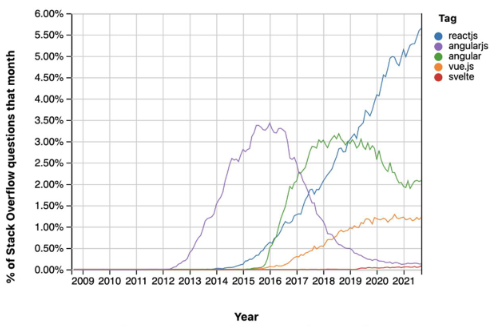
\includegraphics[width=0.85\textwidth]{images/framework_popularity.png}
	\caption{zeigt die Popularität verschiedener Frontend-Frameworks über die Jahre, basierend auf dem Anteil der Fragen auf Stack Overflow. \textit{\cite{akivab_js_framework}}}
\end{figure}


\subsubsection{Angular}

\textbf{Einführung in Angular}
\newline
Angular ist ein quelloffenes Framework für die Frontend-Webentwicklung, das von Google entwickelt wurde. Es wurde erstmals 2010 als AngularJS eingeführt und mit Angular 2 vollständig überarbeitet. Es basiert auf TypeScript und ermöglicht die Erstellung dynamischer, skalierbarer Single-Page-Anwendungen (SPAs). Durch regelmäßige Updates bleibt Angular ein modernes Framework, das an die Anforderungen der Webentwicklung angepasst ist.\textit{\cite{madurapperuma2022state, shetty2020review, angular}} \newline


\textbf{Architektur}
\newline
Angular verwendet eine komponentenbasierte Architektur, bei der die Benutzeroberfläche in kleine, wiederverwendbare Teile (Komponenten) unterteilt wird. Jede Komponente besteht aus:

\begin{itemize}
	\item \textbf{Templates}: HTML, erweitert mit Angular-spezifischen Direktiven.
	\item \textbf{Styles}: CSS oder SCSS für das Design.
	\item \textbf{Logik}: TypeScript für die Geschäftslogik.
\end{itemize}

Komponenten werden in Modulen (\text{NgModules}) gruppiert, um eine bessere Organisation und Wiederverwendbarkeit zu gewährleisten. Diese Struktur fördert die Modularität und erleichtert die Wartung des Codes.\textit{\cite{hutagikar2020analysis, shetty2020review, angular}} \newline

\textbf{Hauptfunktionen von Angular}

\textbf{Datenbindung} 

Angular unterstützt sowohl Einweg- als auch Zweiweg-Datenbindung:

\begin{itemize}
	\item \textbf{Einweg-Datenbindung}: Daten fließen nur vom Model zur View.
	\item \textbf{Zweiweg-Datenbindung}: Änderungen in der View werden automatisch an das Model zurückgegeben und umgekehrt. Dies wird häufig für Formulare verwendet und reduziert den manuellen Aufwand bei der Synchronisation.\textit{\cite{hutagikar2020analysis, madurapperuma2022state, angular}}
\end{itemize}

\textbf{Vorteile von Angular}
\begin{itemize}
	\item \textbf{Skalierbarkeit}: Angular eignet sich sowohl für kleine als auch für große Projekte, dank seiner Modularität und TypeScript-Unterstützung.\textit{\cite{madurapperuma2022state, rathinam2022analysis, angular}}
	
	\item \textbf{Integrierte Tools}: Angular CLI (Command Line Interface) erleichtert die Projektinitialisierung, den Build-Prozess und das Testen. Angular Material bietet vorgefertigte UI-Komponenten, die das Design beschleunigen.\textit{\cite{hutagikar2020analysis, angular_blog}}
	
	\item \textbf{Community und Support}: Als von Google unterstütztes Framework verfügt Angular über eine aktive Entwicklergemeinschaft, regelmäßige Updates und umfassende Dokumentation.\textit{\cite{shetty2020review, angular}}
\end{itemize}

\textbf{Nachteile von Angular}
\begin{itemize}
	\item \textbf{Steile Lernkurve}: Durch die Einführung von TypeScript, Dependency Injection und einer komplexen Struktur ist Angular für Anfänger herausfordernd.\textit{\cite{madurapperuma2022state, rathinam2022analysis, angular_blog}}
	\item \textbf{Framework-Größe}: Angular ist im Vergleich zu leichtgewichtigen Frameworks wie Vue.js oft schwerer und kann dadurch die Ladezeit beeinflussen.\textit{\cite{shetty2020review, angular}}
\end{itemize}


\subsubsection{React}

\textbf{Einführung in React}
\newline
React ist eine quelloffene JavaScript-Bibliothek, die von Meta (ehemals Facebook) entwickelt wurde und hauptsächlich zur Erstellung von Benutzeroberflächen verwendet wird. Sie wurde erstmals 2013 veröffentlicht und ist besonders für die Entwicklung dynamischer Single-Page-Anwendungen (SPAs) geeignet. React basiert auf dem Konzept von Komponenten und der Verwendung eines virtuellen DOM, um die Performance zu optimieren. Es bietet eine flexible Architektur für die Entwicklung moderner Webanwendungen.\textit{\cite{rathinam2022analysis, hutagikar2020analysis, react}} \newline

\textbf{Architektur}
\newline
React verwendet eine komponentenbasierte Architektur, bei der Benutzeroberflächen in kleinere, wiederverwendbare Teile aufgeteilt werden. Diese Architektur ermöglicht eine einfache Wartung und Erweiterung von Anwendungen. Jede Komponente in React ist in JSX (JavaScript XML) geschrieben, einer Syntaxerweiterung, die HTML-ähnlichen Code innerhalb von JavaScript erlaubt.

\begin{itemize}
	\item \textbf{Virtueller DOM}: React verwendet einen virtuellen DOM, der Änderungen an der Benutzeroberfläche effizient berechnet und nur die betroffenen Teile des echten DOM aktualisiert.
	\item \textbf{JSX}: JSX ist eine Mischung aus JavaScript und HTML, die es Entwicklern ermöglicht, benutzerdefinierte UI-Komponenten zu erstellen.
	\item \textbf{Unidirektionaler Datenfluss}: Daten fließen in React in einer einzigen Richtung, was die Verwaltung und Nachverfolgbarkeit von Daten einfacher macht.\textit{\cite{rathinam2022analysis, hutagikar2020analysis, react}}
\end{itemize}

\textbf{Hauptfunktionen von React}

\textbf{Komponentenbasierte Entwicklung} 

React ermöglicht die Erstellung von wiederverwendbaren und modularen Komponenten, die sowohl die Benutzeroberfläche als auch die Logik kapseln. Dies fördert eine bessere Strukturierung und Wartbarkeit des Codes.\textit{\cite{shetty2020review, react}}

\textbf{Virtueller DOM} 

Der virtuelle DOM verbessert die Performance von React-Anwendungen, indem er Änderungen effizient berechnet und nur die betroffenen Teile des echten DOM aktualisiert. Dies reduziert die Anzahl der direkten DOM-Manipulationen erheblich.\textit{\cite{rathinam2022analysis, hutagikar2020analysis, react}}

\textbf{Vorteile von React}
\begin{itemize}
	\item \textbf{Performance}: Der virtuelle DOM und die asynchrone Verarbeitung ermöglichen eine schnelle und effiziente Benutzeroberfläche.\textit{\cite{rathinam2022analysis, react}}
	
	\item \textbf{Flexibilität und Wiederverwendbarkeit}: Die komponentenbasierte Architektur von React erleichtert die Wiederverwendung von Code und die Skalierung von Anwendungen.\textit{\cite{hutagikar2020analysis, react}}
	
	\item \textbf{Große Community und Ökosystem}: React wird von einer riesigen Entwicklergemeinschaft unterstützt, und es gibt zahlreiche Bibliotheken und Tools, die den Entwicklungsprozess verbessern.\textit{\cite{shetty2020review, react}}
\end{itemize}

\textbf{Nachteile von React}
\begin{itemize}
	\item \textbf{Zusätzliche Abhängigkeiten}: React bietet nur die grundlegende Architektur, weshalb oft zusätzliche Bibliotheken (z. B. für Routing oder State Management) benötigt werden.\textit{\cite{shetty2020review, rathinam2022analysis, react_blog}}
	
	\item \textbf{Lernkurve}: Für Entwickler, die mit JSX und der Unidirektionalität des Datenflusses nicht vertraut sind, kann React eine gewisse Lernkurve darstellen.\textit{\cite{hutagikar2020analysis, react_blog}}
\end{itemize}



\subsubsection{Vue.js}

\textbf{Einführung in Vue.js}
\newline
Vue.js ist ein progressives JavaScript-Framework, das 2014 von Evan You entwickelt wurde. Es wird häufig für die Erstellung von Benutzeroberflächen und Single-Page-Anwendungen (SPAs) verwendet. Vue.js zeichnet sich durch seine einfache Integration in bestehende Projekte und seine Flexibilität aus, wodurch es sowohl für kleine als auch große Anwendungen geeignet ist. Durch seine modulare Struktur und starke Community-Unterstützung bleibt Vue.js ein beliebtes Framework für Webentwickler.\textit{\cite{rathinam2022analysis, madurapperuma2022state, vuejs}} \newline

\textbf{Architektur}
\newline
Vue.js verwendet die Model-View-ViewModel (MVVM)-Architektur, die es ermöglicht, die Benutzeroberfläche, die Geschäftslogik und die Datenbindung effizient zu verwalten. Die Hauptbestandteile von Vue.js sind:

\begin{itemize}
	\item \textbf{Templates}: Vue.js verwendet Templates, um UI-Komponenten zu definieren. Diese Templates werden in renderbare DOM-Elemente übersetzt.
	\item \textbf{Reaktivitätssystem}: Das reaktive Datenmodell von Vue.js ermöglicht automatische Updates der Benutzeroberfläche, wenn sich die zugrunde liegenden Daten ändern.
	\item \textbf{Direktiven}: Vue.js bietet spezielle HTML-Attribute (Direktiven), die Funktionen wie Schleifen, Bedingungen und Ereignishandlungen erleichtern.\textit{\cite{hutagikar2020analysis, vuejs}}
\end{itemize}

\textbf{Hauptfunktionen von Vue.js}

\textbf{Komponentenbasierte Entwicklung} 

Wie React und Angular ermöglicht Vue.js die Erstellung von wiederverwendbaren und modularen Komponenten. Diese Struktur fördert die Organisation und erleichtert die Wartung und Erweiterung von Anwendungen.\textit{\cite{rathinam2022analysis, vuejs}}

\textbf{Reaktivitätssystem} 

Das Reaktivitätssystem von Vue.js überwacht automatisch Änderungen im Datenmodell und aktualisiert die Benutzeroberfläche entsprechend. Dies macht die manuelle DOM-Manipulation überflüssig und verbessert die Entwicklererfahrung.\textit{\cite{hutagikar2020analysis, vue_blog}}

\textbf{Vorteile von Vue.js}
\begin{itemize}
	\item \textbf{Einfache Lernkurve}: Vue.js ist einfach zu lernen, da es eine klare und intuitive Syntax bietet. Es ist besonders für Entwickler geeignet, die mit HTML, CSS und JavaScript vertraut sind.\textit{\cite{madurapperuma2022state, vuejs}}
	
	\item \textbf{Flexibilität und Modularität}: Vue.js kann sowohl für einfache Widgets als auch für komplexe Anwendungen verwendet werden. Seine modulare Struktur ermöglicht eine einfache Integration in bestehende Projekte.\textit{\cite{rathinam2022analysis, vuejs}}
	
	\item \textbf{Leichtgewichtig und performant}: Vue.js ist kleiner als Frameworks wie Angular und React, was die Ladezeit reduziert und die Performance verbessert.\textit{\cite{shetty2020review, vuejs}}
\end{itemize}

\textbf{Nachteile von Vue.js}
\begin{itemize}
	\item \textbf{Geringere Unterstützung durch große Unternehmen}: Im Gegensatz zu React und Angular wird Vue.js nicht von einer großen Organisation unterstützt, was in einigen Fällen zu Unsicherheiten führen kann.\textit{\cite{rathinam2022analysis, vue_blog}}
	
	\item \textbf{Weniger umfangreiches Ökosystem}: Während Vue.js eine starke Community hat, sind bestimmte Drittanbieter-Bibliotheken und Tools im Vergleich zu React und Angular weniger verbreitet.\textit{\cite{hutagikar2020analysis, vue_blog}}
\end{itemize}


\subsubsection{Next.js}

\textbf{Einführung in Next.js}
\newline Next.js ist ein populäres Open-Source-React-Framework, das 2016 von Vercel entwickelt wurde. Es erleichtert die Erstellung von Server-Rendered-Anwendungen und bietet Funktionen wie statische Seitengenerierung, serverseitiges Rendering und dynamisches Routing. Mit seiner Optimierung für Entwicklererfahrung und seiner Flexibilität ist Next.js eine bevorzugte Wahl für moderne Webprojekte und eignet sich sowohl für einfache als auch komplexe Anwendungen. Dank seiner Performance-Vorteile und Integration mit React bleibt es eine wichtige Technologie im Bereich der Webentwicklung.\textit{\cite{nextjs, rathinam2022analysis, shetty2020review}}

\textbf{Architektur}
\newline Next.js verwendet eine komponentenbasierte Architektur, die auf React aufbaut und eine erweiterte Struktur zur effizienten Verwaltung von Benutzeroberflächen und Backend-Interaktionen bereitstellt. Die Hauptbestandteile von Next.js sind:
\begin{itemize} \item \textbf{Pages und Routing}: Jede Datei in der \texttt{pages}-Ordnerstruktur entspricht einer Route. Next.js unterstützt sowohl statische als auch dynamische Routen. \item \textbf{Serverseitiges Rendering (SSR)}: Ermöglicht die Generierung von Inhalten auf dem Server, bevor sie an den Client gesendet werden. \item \textbf{Statische Seitengenerierung (SSG)}: Statische Seiten werden zur Build-Zeit generiert, was die Performance und SEO optimiert.\textit{\cite{nextjs, nextjs_blog, rathinam2022analysis}} \end{itemize}

\textbf{Hauptfunktionen von Next.js}

\textbf{Server-Rendering und Statische Generierung}
Next.js kombiniert serverseitiges Rendering und statische Seitengenerierung, um Entwicklern die Flexibilität zu bieten, die beste Strategie für ihre Anwendung zu wählen. Diese Funktionen fördern die Performance und SEO.\textit{\cite{nextjs, nextjs_blog, shetty2020review}}

\textbf{Integrierte Optimierungen}
Next.js bietet Funktionen wie automatisches Code-Splitting, \newline
Image-Optimierung und automatische Routing-Updates, die eine effiziente und moderne Entwicklungserfahrung fördern.\textit{\cite{nextjs, rathinam2022analysis, nextjs_blog}}

\textbf{Vorteile von Next.js}
\begin{itemize} \item \textbf{SEO-Optimierung}: Server-Rendering und statische Generierung tragen zur Verbesserung der Suchmaschinenplatzierung bei.\textit{\cite{nextjs, nextjs_blog, shetty2020review}} \item \textbf{Hohe Performance}: Durch Funktionen wie automatische Code-Splitting und Bildoptimierung bietet Next.js schnelle Ladezeiten und eine optimale Benutzererfahrung.\textit{\cite{rathinam2022analysis, nextjs, shetty2020review}} \item \textbf{Flexibilität}: Die Unterstützung für verschiedene Rendering-Strategien und die Integration mit React ermöglichen den Einsatz für eine Vielzahl von Anwendungsfällen.\textit{\cite{nextjs_blog, nextjs, shetty2020review}} \end{itemize}

\textbf{Nachteile von Next.js}
\begin{itemize} \item \textbf{Steile Lernkurve}: Insbesondere für Entwickler ohne Erfahrung mit React kann die Einarbeitung in Next.js herausfordernd sein.\textit{\cite{rathinam2022analysis, shetty2020review}} \item \textbf{Build-Zeiten}: Bei sehr großen Projekten können die Build-Zeiten länger dauern, was die Entwicklungszyklen beeinflusst.\textit{\cite{madurapperuma2022state, rathinam2022analysis}} \end{itemize}




% Dokumente für Machbarkeit

\chapter{Technische Machbarkeitsstudie}

\setauthor{Manuel Fellner}
\section{Technische Machbarkeit des Backends}
\subsection{Kriterien}
Die Wahl der Kriterien für die Bewertung der Backend-Technologien basiert auf den spezifischen Anforderungen des Projekts. Jedes Kriterium spiegelt eine entscheidende Eigenschaft wider, die den Erfolg der Umsetzung maßgeblich beeinflusst. Die Gewichtung erfolgte in enger Abstimmung mit den Projektzielen und Anforderungen.
\begin{enumerate}
	\item Einfache Implementierung (15 \%): Wie einfach ist die Technologie aufzusetzen und zu implementieren?
	\item Aktuelle Sprachkenntnisse (20 \%): Welche Programmiersprache dominiert die Technologie? Wird diese bereits vom Projektteam beherrscht?
	\item Skalierbarkeit (10 \%): Wie einfach sind bereits vorhandene Applikationen mit der Technologie im Nachhinein zu skalieren?
	\item Sicherheit (10 \%): Welche Sicherheitsfunktionen stellen diese Technologien bereit? Sind diese bereits automatisch vorhanden, oder müssen sie manuell implementiert werden?
	\item Performance (10 \%): Wie schnell ist die Applikation in der Lage, Anfragen zu verarbeiten? Wie geht diese mit einer größeren Skalierung umher?
	\item Community und Support (10 \%): Wie aktiv ist die Community? Bietet der Hersteller von sich aus einen Support an, oder muss man sich dafür an Dritte wenden?
	\item Dokumentation (10 \%): Ist eine Herstellereigene Dokumentation vorhanden? Wie umfangreich und gepflegt ist diese?
	\item Integration mit Frontend \& Datenbank (10 \%): Wie gut ist die Technologie mit den gängigsten Frontend-/Datenbankframeworks kompatibel?
    \item Verfügbarkeit von Libraries (5 \%): Wie viele Drittanbieter-Bibliotheken stehen zur Verfügung? Welchen Funktionsumfang bieten sie an?
\end{enumerate}

Die Gewichtung der Kriterien spiegelt die spezifischen Anforderungen des Projekts wider. Die höchste Priorität wurde auf die Sprachkenntnisse und Implementierung gelegt, um die Effizienz der Entwicklung im schulischen Rahmen zu gewährleisten. Skalierbarkeit und Sicherheit wurden hoch gewichtet, da diese Aspekte entscheidend für die langfristige Nutzbarkeit des Systems sind. Performance, Community und Support, Dokumentation sowie eine einfache Integration mit verschiedenen Frontend- und Datenbanksystemen werden als unterstützende, aber nicht zentrale Faktoren betrachtet.

Um die Analyse der jeweiligen Technologien authentischer zu machen, wurden für den praktischen Teil die folgenden Vorstudienszenarien aufgestellt:

\begin{itemize}
	\item Das Aufsetzen eines Projektes mit der jeweiligen Technologie
	\item Das Erstellen einer simplen REST-Schnittstelle mit der jeweiligen Technologie
\end{itemize}

\subsection{Ergebnisse}

\subsubsection{Django}

Beim Aufsetzen eines Projekts mit Django wurde festgestellt, dass der Initialisierungsprozess durch das Kommandozeilenwerkzeug \texttt{django-admin} (welches in \cite{website-django-admin} dokumentiert wurde) stark vereinfacht wird. Durch Ausführen des Befehls \texttt{django-admin startproject} wurde eine grundlegende Projektstruktur automatisch generiert. Diese vordefinierte Struktur umfasste wichtige Verzeichnisse und Konfigurationsdateien, wodurch die Einrichtungsphase beschleunigt wurde. Diese automatische Einstellung ermöglicht einen schnellen Einstieg in die Entwicklung.

Für die Erstellung einer REST-Schnittstelle wurde das Django REST Framework verwendet. Dabei wurde eine API-Endpunktstruktur implementiert, \gls{CRUD} Operationen für einen einfachen Datensatz ermöglichte. Es zeigte sich, dass durch die Nutzung des Django REST Frameworks viele notwendige Funktionen wie Serialisierung und Validierung bereits als vordefinierte Module verfügbar sind, jedoch viel Vorkenntnisse benötigen, um effizient genutzt werden zu können. Dies erhöhte den Implementierungsaufwand. Der API-Endpunkt konnte erfolgreich getestet werden, wobei eine JSON-Ausgabe über die integrierte Entwicklungsumgebung von Django bereitgestellt wurde.

\subsubsection{Flask}

Beim Aufsetzen eines Projekts mit Flask wurde ein minimalistischer Ansatz festgestellt, da kein automatisches Generieren einer Projektstruktur angeboten wird. Stattdessen mussten die erforderlichen Verzeichnisse und Dateien manuell erstellt werden. Als Einstiegspunkt wurde ein grundlegendes Python-Skript eingerichtet, das als Hauptdatei der Anwendung diente. Diese manuelle Vorgehensweise bietet zwar mehr Kontrolle über die Projektstruktur, führt jedoch auch zu einem erhöhten Konfigurationsaufwand.

Für die Erstellung einer REST-Schnittstelle kam die Bibliothek \texttt{flask} zum Einsatz. Ein einfacher API-Endpunkt wurde definiert, der sowohl HTTP-GET- als auch POST-Anfragen verarbeiten konnte. Die Implementierung erfolgte durch das Hinzufügen einer Route innerhalb der Python-Datei, die eine JSON-Antwort zurückgab. Dabei wurde festgestellt, dass die REST-Schnittstelle mit minimalem Code und ohne zusätzliche Abhängigkeiten umgesetzt werden konnte. Die Flexibilität von Flask erlaubte es, die API-Logik schnell und unkompliziert anzupassen. Allerdings wurde festgestellt, dass Sicherheitsfunktionen und Validierungen manuell implementiert werden müssen, was zusätzlichen Entwicklungsaufwand erfordert.


\subsubsection{ExpressJS}

Beim Aufsetzen eines Projekts mit ExpressJS wurde das Kommandozeilenwerkzeug \texttt{npm}, welches unter \cite{website-npm} genauer dokumentiert wurde, verwendet, um ein neues Projekt zu initialisieren. Der Befehl \texttt{express-generator} (siehe \cite{website-expressjs-generator}) generierte dabei automatisch eine grundlegende Projektstruktur. Diese Struktur umfasste vordefinierte Verzeichnisse für Routen, Ansichten und öffentliche Dateien, wodurch der Entwicklungsprozess erheblich vereinfacht wurde. Nach der Installation der erforderlichen Abhängigkeiten konnte das Projekt lokal gestartet und weiterentwickelt werden.

Für die Implementierung einer REST-Schnittstelle wurde eine einfache Route definiert, die HTTP-Anfragen verarbeiten und JSON-Daten zurückgeben konnte. Der ExpressJS-Server konnte dabei mit nur wenigen Zeilen Code konfiguriert werden. Um die Verarbeitung von Anfrageinhalten zu erleichtern, wurden externe Bibliotheken wie die Middleware \texttt{body-parser} (siehe \cite{website-expressjs-body-parser-lib}) integriert. Die entwickelte REST-Schnittstelle wurde erfolgreich getestet, indem sowohl GET- als auch POST-Anfragen an den API-Endpunkt gesendet wurden. Während der Tests zeigte sich, dass ExpressJS durch seine asynchrone Architektur besonders gut für die Verarbeitung paralleler Anfragen geeignet ist, sofern die entsprechende Funktionalität im Quellcode korrekt implementiert wird. Die Programmierung sowie das damit verbundene Debugging können bei dieser Technologie etwas aufwendiger sein, da JavaScript eine sehr spezielle Programmiersprache ist.


\subsubsection{Spring Boot}

Das Projekt wurde unter Verwendung des Tools \textit{Spring Initializr}, der auf \cite{website-spring-initializr} gefunden werden kann, aufgesetzt. Dieses bietet eine benutzerfreundliche Weboberfläche zur automatisierten Generierung einer projektbasierten Verzeichnisstruktur. Nach der Auswahl relevanter Abhängigkeiten und Funktionalitäten konnten die erstellten Dateien als ZIP-Archiv heruntergeladen werden. Durch diesen automatisierten Setup-Prozess wurde der Einstieg in die Entwicklung deutlich beschleunigt. Nach dem Entpacken der Dateien wurde das Projekt in einer geeigneten Entwicklungsumgebung, wie beispielsweise IntelliJ IDEA, geöffnet und weiterentwickelt.

Im Rahmen der Implementierung der REST-Schnittstelle wurde eine einfache Controller-Klasse erstellt, die einen API-Endpunkt bereitstellt. Dieser Endpunkt war in der Lage, HTTP-Anfragen entgegenzunehmen und JSON-Antworten zu liefern. Dabei zeigte sich, dass Spring Boot umfangreiche Funktionalitäten wie Validierung, Serialisierung und Fehlerbehandlung bereits integriert hat, wodurch sich der Entwicklungsaufwand signifikant reduzierte. Die entwickelte REST-Schnittstelle wurde mittels GET- und POST-Anfragen erfolgreich getestet. Es konnte eine hohe Stabilität und Performance von Spring Boot beobachtet werden, insbesondere bei der Verarbeitung paralleler Anfragen.


\subsection{Bewertung und Auswahl}

Die einzelnen Technologien wurden im letzten Schritt isoliert voneinander begutachtet, nun folgt der direkte Vergleich.

\subsubsection{Django}

Django bietet eine solide Projektstruktur, die durch den Befehl \texttt{django-admin startproject}, siehe \cite{website-django-admin}, automatisch generiert wird. Die einfache Implementierung wird jedoch durch die Notwendigkeit umfangreicher Vorkenntnisse relativiert. Das Django REST Framework reduziert den Implementierungsaufwand durch integrierte Serialisierungs- und Validierungsfunktionen. Django zeigte Stärken in der Community-Unterstützung und Performance, jedoch erhöhten die hohen Anforderungen an die Konfiguration den Aufwand in der Praxis.

\subsubsection{Flask}

Flask verfolgt einen minimalistischen Ansatz und ermöglicht eine flexible Anpassung der Projektstruktur. Diese Flexibilität führte zu einer höheren Punktzahl bei der einfachen Implementierung, da weniger Vorgaben zu beachten sind. Jedoch müssen Sicherheitsfunktionen und Validierungen manuell implementiert werden, was zusätzlichen Aufwand erfordert. Flask punktete vor allem durch seine Performance und einfache Anpassbarkeit der API-Logik, fiel jedoch bei der Community-Unterstützung etwas ab.

\subsubsection{ExpressJS}

ExpressJS bietet durch den \texttt{express-generator}, welcher unter \cite{website-expressjs-generator} zu finden ist, eine einfache Möglichkeit, eine Projektstruktur schnell aufzusetzen. Die Technologie zeigte gute Ergebnisse bei der Skalierbarkeit und der einfachen Implementierung, jedoch sind Programmierung und Debugging aufgrund der Besonderheiten von JavaScript teilweise aufwendiger. ExpressJS punktete besonders in der Performance und bei parallelen Anfragen, während es in der Community-Unterstützung und Dokumentation solide Ergebnisse lieferte.

\subsubsection{Spring Boot}

Spring Boot erwies sich als die leistungsstärkste Lösung unter den analysierten Technologien. Die Verwendung des \textit{Spring Initializr} ermöglichte einen schnellen Einstieg in die Projektentwicklung. Spring Boot integrierte umfangreiche Funktionen wie Validierung, Serialisierung und Fehlerbehandlung, was den Implementierungsaufwand erheblich reduzierte. Die Technologie punktete stark bei der Skalierbarkeit und der Performance, insbesondere bei parallelen Anfragen. Zudem profitierte Spring Boot von einer umfangreichen Community und ausgezeichneten Dokumentation.

\subsection{Analytische Nutzwertanalyse}

Nun bewerten wir die jeweilige Technologie mit einem einfachen Punktesystem. Hierbei bedeutet die Zahl \texttt{1} die schlechteste, und die Zahl \texttt{5} die bestmögliche Bewertung.

\begin{table}[H]
	\centering
	\renewcommand{\arraystretch}{1.2}
	\begin{tabular}{|l|c|c|c|c|c|}
		\hline
		\rowcolor[HTML]{B6D7A8} \textbf{Kriterium} & \textbf{Gewichtung (\%)} & \textbf{Django} & \textbf{Flask} & \textbf{ExpressJs} & \textbf{Spring Boot} \\
		\hline
		Einfache Implementierung & 15 & 4 & 5 & 4 & 4 \\
		\hline
		Aktuelle Sprachkenntnisse & 20 & 3 & 5 & 3 & 4 \\
		\hline
		Skalierbarkeit & 10 & 4 & 3 & 4 & 5 \\
		\hline
		Community und Support & 10 & 5 & 3 & 3 & 4 \\
		\hline
		Performance & 10 & 3 & 5 & 4 & 5 \\
		\hline
		Sicherheit & 10 & 5 & 3 & 3 & 5 \\
		\hline
		Integration mit Frontend \& DB & 10 & 4 & 4 & 4 & 4 \\
		\hline
		Vorhandene Dokumentation & 10 & 5 & 3 & 3 & 5 \\
		\hline
		Verfügbarkeit von Libraries & 5 & 5 & 4 & 5 & 4 \\
		\hline
	\end{tabular}
	\caption{Nutzwertanalyse der Backend-Technologien: Bewertung der Datenbanken nach verschiedenen Kriterien. (wobei 5 = Sehr gut, 1 = Sehr schlecht) (Prompt \cite{prompt-gpt-google-sheets-to-table})}
    \label{table-analytische-nwa-backend}
\end{table}

Tabelle \ref{table-analytische-nwa-backend} zeigt, dass die jeweiligen Technologien dementsprechend ihre Stärken und Schwächen besitzen. Während zum Beispiel Flask mit einer einfachen Implementierung punkten kann, ist es, was die Sicherheit angeht, z.B. Spring Boot und Django unterlegen.

\begin{table}[H]
	\centering
	\renewcommand{\arraystretch}{1.2}
	\begin{tabular}{|l|c|c|c|c|}
		\hline
		\rowcolor[HTML]{B6D7A8} & \textbf{Django} & \textbf{Flask} & \textbf{ExpressJs} & \textbf{Spring Boot} \\
		\hline
		Einfache Implementierung & 0.6 & 0.75 & 0.6 & 0.6 \\
		\hline
		Aktuelle Sprachkenntnisse & 0.6 & 1 & 0.6 & 0.8 \\
		\hline
		Skalierbarkeit & 0.4 & 0.3 & 0.4 & 0.5 \\
		\hline
		Community und Support & 0.5 & 0.3 & 0.3 & 0.4 \\
		\hline
		Performance & 0.3 & 0.5 & 0.4 & 0.5 \\
		\hline
		Sicherheit & 0.5 & 0.3 & 0.3 & 0.5 \\
		\hline
		Integration mit Frontend \& DB & 0.4 & 0.4 & 0.4 & 0.4 \\
		\hline
		Vorhandene Dokumentation & 0.5 & 0.3 & 0.3 & 0.5 \\
		\hline
		Verfügbarkeit von Libraries & 0.25 & 0.2 & 0.25 & 0.2 \\
		\hline
		\textbf{GESAMTERGEBNIS} & \textbf{4.05} & \textbf{4.05} & \textbf{3.55} & \textbf{4.4} \\
		\hline
	\end{tabular}
	\caption{Zusammenzählung der einzelnen Bewertungen anhand der in Tabelle \ref{table-analytische-nwa-backend} gegebenen Punkte. Hierbei gilt: je höher, desto besser. (Prompt \cite{prompt-gpt-google-sheets-to-table})}
    \label{table-analytische-nwa-backend-result}
\end{table}

Wie in der Tabelle \ref{table-analytische-nwa-backend-result} dargestellt, ist \texttt{Spring Boot} mit einer Punktzahl von \texttt{4.4} der Gewinner. Daher werden wir in diesem Projekt diese Technologie auch für die Backend-Entwicklung verwenden.

Basierend auf der durchgeführten Nutzwertanalyse erweist sich \textbf{Spring Boot} als die optimale Technologie für die Backend-Entwicklung dieses Projekts. Spring Boot überzeugt durch seine einfache Implementierung, umfangreiche Sicherheitsfunktionen und hervorragende Skalierbarkeit. Das bestehende Know-how im Projektteam hinsichtlich der Programmiersprache Java ermöglicht eine effiziente Nutzung des Frameworks.

Im Vergleich zu den alternativen Technologien punktet Spring Boot vor allem durch seine service-orientierte Architektur und die Integration wesentlicher Funktionen wie Validierung und Serialisierung. Django, Flask und ExpressJS bieten zwar interessante Ansätze, konnten jedoch in den bewerteten Kriterien nicht in gleichem Maße überzeugen.

Insgesamt stellt Spring Boot die stabilste und zukunftssicherste Lösung dar und wird daher für die Umsetzung des Projekts verwendet.

\setauthor{Sebastian Sailer}
\section{Technische Machbarkeit der Datenbank}
\subsection{Methodik}

Die im vorherigen Kapitel beschriebenen DBMS werden in diesem Abschnitt detailliert untersucht, miteinander verglichen und bewertet. Dabei erfolgt die Beurteilung anhand der folgenden acht Kriterien: Leistungsfähigkeit, Skalierbarkeit, Wirtschaftlichkeit, Unterstützung durch Community und Support, Verfügbarkeit, Sicherheit, Anpassungsfähigkeit sowie der Dokumentation.

\subsection{Bewertung der Datenbanktechnologien}

Die Wahl der Kriterien für die Bewertung von Datenbanktechnologien basiert auf den spezifischen Anforderungen des Projekts. Jedes Kriterium repräsentiert eine wesentliche Eigenschaft, die maßgeblich zur erfolgreichen Implementierung einer Datenbanklösung beiträgt. Die Gewichtung der Kriterien erfolgte in Abstimmung mit den Projektzielen und der vorgesehenen Nutzung der Datenbank.

\begin{itemize}
	\item \textbf{Performance (20\%)}: 
	Die Fähigkeit der Datenbank, schnell auf Anfragen zu reagieren und große Datenmengen effizient zu verarbeiten.
	
	\item \textbf{Skalierbarkeit (15\%)}: 
	Eine Datenbank muss problemlos mit einem wachsenden Datenvolumen und einer steigenden Anzahl von Nutzern umgehen können, ohne dass die Leistung stark beeinträchtigt wird.
	
	\item \textbf{Kosten (10\%)}: 
	Die Wirtschaftlichkeit einer Lösung ist ein zentraler Faktor, insbesondere in Bezug auf Lizenzgebühren, Betriebskosten und mögliche Einsparungen durch Open-Source-Lösungen. Eine kosteneffiziente Lösung ist ein wichtiger Punkt des Auftraggebers.
	
	\item \textbf{Community und Support (10\%)}: 
	Eine aktive Community erleichtert die Lösung technischer Probleme und gewährleistet die kontinuierliche Weiterentwicklung der Technologie.
	
	\item \textbf{Verfügbarkeit (10\%)}: 
	Die Datenbank muss eine hohe Verfügbarkeit und Zuverlässigkeit gewährleisten, um Betriebsunterbrechungen zu vermeiden.
	
	\item \textbf{Sicherheit (15\%)}: 
	Der Schutz sensibler Daten vor unbefugtem Zugriff und Cyberangriffen ist unerlässlich. Dazu zählen Mechanismen wie Verschlüsselung, Zugangskontrollen und regelmäßige Sicherheitsupdates.
	
	\item \textbf{Flexibilität (10\%)}: 
	Die Datenbank sollte anpassbar sein und verschiedene Datenmodelle sowie Integrationen unterstützen, um unterschiedlichen Anforderungen gerecht zu werden und in Zukunft erweiterbar zu sein.
	
	\item \textbf{Dokumentation und Verwaltung (10\%)}: 
	Eine klare und umfassende Dokumentation sowie benutzerfreundliche Verwaltungswerkzeuge sind essenziell, um das Aufsetzen als auch die Bedienung und Wartung der Datenbank zu erleichtern.
\end{itemize}

\noindent Die Gewichtung dieser Kriterien spiegelt die spezifischen Anforderungen des Projekts wider. Die höchsten Prioritäten wurden auf Performance und Skalierbarkeit gelegt, da sie die Grundlage und den Sinn des Projektes bilden. Sicherheit ist ebenfalls von zentraler Bedeutung, um den Schutz sensibler Daten zu gewährleisten und rechtliche Vorgaben einzuhalten. Aspekte wie Community und Support, Verfügbarkeit, Flexibilität sowie Dokumentation und Verwaltung werden als unterstützende, aber nicht primäre Faktoren betrachtet. 

\vspace{3mm}
\noindent Der Auftraggeber wünschte eine möglichst kosteneffiziente Arbeitsweise, weshalb entschieden wurde, eine Open-Source-Lösung zu bevorzugen. Dennoch wurde ein kostenpflichtiges DBMS in die Analyse einbezogen, um potenzielle Vorteile, einschließlich finanzieller Aspekte, zu bewerten und einen umfassenden Vergleich zu ermöglichen. (Prompt \cite{ChatGPT:rewrite2})

\subsection{Ergebnisse}

Die analysierten Datenbanktechnologien wurden basierend auf den Kriterien Performance, Skalierbarkeit, Kosten, Community und Support, Verfügbarkeit, Sicherheit, Flexibilität, Dokumentation und Verwaltung bewertet. Im Folgenden werden die Ergebnisse der Untersuchung für die einzelnen Technologien dargestellt. Ziel war es, die für das Projekt am besten geeignete Lösung zu identifizieren, die sowohl den technischen Anforderungen als auch den finanziellen Rahmenbedingungen entspricht.

\subsubsection{PostgreSQL}
PostgreSQL erwies sich als eine leistungsfähige und vielseitige Open-Source-Datenbank. Laut dem Paper \cite{Paper:performanceComparison} bietet sie eine hervorragende Performance bei komplexen Abfragen und eignet sich besonders gut für Anwendungen, die große Datenmengen verarbeiten. Auch in Bezug auf die Skalierbarkeit zeigt PostgreSQL klare Stärken: Bei der vertikalen Skalierung kann die Leistung durch den Ausbau von Hardware-Ressourcen wie CPU, Arbeitsspeicher oder Speicherplatz verbessert werden – was vergleichsweise einfach umzusetzen ist. Horizontale Skalierung hingegen bedeutet, die Last auf mehrere Server zu verteilen, was in PostgreSQL beispielsweise durch Replikation oder den Einsatz von Tools wie zum Beispiel Citus realisierbar ist. Die aktive Community sowie eine gute Dokumentation erleichtern sowohl die Einarbeitung als auch den zuverlässigen Betrieb. Zudem überzeugt PostgreSQL durch seine kostenfreie Verfügbarkeit und starke Sicherheitsfunktionen. 

\subsubsection{MariaDB}
MariaDB, eine ebenfalls weit verbreitete Open-Source-Datenbank, überzeugte mit solider Performance, die jedoch insbesondere bei leseintensiven Anwendungen und einfachen Abfragen nicht ganz das Niveau von MySQL erreicht, siehe \cite{Paper:performanceComparisonMySQL}(Prompt \cite{ChatGPT:rewrite3}).Die Datenbank ist leicht zu verwalten und bietet solide Optionen für die vertikale Skalierung. Jedoch sind die Möglichkeiten für horizontale Skalierung, also das Verteilen von Daten auf mehrere Knotenpunkte, begrenzt. Im Gegenzug zu PostgreSQL stößt MariaDB hier an seine Grenzen. Dennoch ist MariaDB dank ihrer einfachen Verwaltung, einer großen Community und guter Dokumentation besonders gut für kleine bis mittelgroße Projekte geeignet. Die kostenlose Community-Edition ist für die meisten Anforderungen ausreichend, während die Enterprise-Edition zusätzliche kostenpflichtige Features bereitstellt. \textit{\cite{Buch:PierreMavro} - Chapter 2, Performance Analysis}

\subsubsection{MongoDB}
MongoDB als NoSQL-Datenbank hebt sich durch ihre hohe Flexibilität, Skalierbarkeit und Performance hervor. Sie eignet sich hervorragend für Anwendungen mit variablen Datenstrukturen und unstrukturierten Daten. Besonders bei großen Datenmengen und häufigen Schreibvorgängen zeigt MongoDB ihre Stärken. Laut \cite{Paper:performanceComparison} ist MongoDB allerdings für relationale Abfragen weniger geeignet und weist im Vergleich zu den anderen Technologien einen höheren Speicherbedarf auf. Die Community-Edition ist kostenlos verfügbar, während die Enterprise-Version zusätzliche Kosten verursacht. 

\subsubsection{Amazon Aurora}
Amazon Aurora, eine vollständig verwaltete Cloud-Datenbank, überzeugte durch ihre hohe Performance und Skalierbarkeit, siehe \cite{Amazon:aurora}. Automatische Backups, Replikationen und Failover-Mechanismen machen Aurora zu einer sehr zuverlässigen Lösung, die insbesondere in Cloud-Umgebungen ihre Stärken ausspielt. Allerdings ist diese Technologie im Vergleich zu den Open-Source-Alternativen mit hohen Kosten verbunden und stark an das AWS-Ökosystem gebunden, was die Flexibilität einschränken kann. 


\subsection{Bewertung}
Die Bewertung der einzelnen Technologien erfolgt anhand eines einfachen Punktesystems, wobei 1 die niedrigste und 5 die höchste erreichbare Punktzahl darstellt.

\vspace{10mm}

\begin{table}[h!]
	\centering
	\begin{tabular}{|l|c|c|c|c|c|}
		\hline
		\rowcolor[HTML]{B6D7A8}
		\textbf{Kriterium} & \textbf{Gewichtung (\%)} & \textbf{PostgreSQL} & \textbf{MariaDB} & \textbf{MongoDB} & \textbf{Aurora} \\ \hline
		
		Performance & 20 & 4 & 5 & 3 & 4 \\ \hline
		Skalierbarkeit & 15 & 4 & 3 & 4 & 5 \\ \hline
		Kosten & 10 & 5 & 5 & 4 & 1 \\ \hline
		Community und Support & 10 & 5 & 5 & 4 & 5 \\ \hline
		Verfügbarkeit & 10 & 4 & 4 & 4 & 5 \\ \hline
		Sicherheit & 15 & 4 & 4 & 3 & 4 \\ \hline
		Flexibilität & 10 & 3 & 4 & 5 & 4 \\ \hline
		Dokumentation und Verwaltung & 10 & 5 & 5 & 3 & 5 \\ \hline
		\textbf{GESAMT} & \textbf{100} & & & & \\ \hline
	\end{tabular}
	\caption{Bewertung der Datenbanken nach verschiedener Kriterien (1 = sehr schlecht | 5 = sehr gut) \cite{ChatGPT:table1}}
\end{table}

\noindent In Tabelle 6.3 wird eine übersichtliche Darstellung der im Rahmen der Machbarkeitsstudie zusammengetragenen Informationen gezeigt. Die Tabelle vergleicht die verschiedenen Systeme anhand der genannten Kriterien, um die optimale Entscheidung treffen zu können.

\newpage
\noindent In Tabelle 6.4 werden die Punkte unter Berücksichtigung der Gewichtung berechnet, wodurch das Ergebnis der Nutzwertanalyse ermittelt wird.

\begin{table}[htbp]
	\centering
	\begin{tabular}{|l|c|c|c|c|}
		\hline
		\rowcolor[HTML]{B6D7A8}
		\textbf{Kriterium} & \textbf{PostgreSQL} & \textbf{MariaDB} & \textbf{MongoDB} & \textbf{Aurora} \\ \hline
		Performance             & 0,8 & 1    & 0,6 & 0,8  \\ \hline
		Skalierbarkeit          & 0,6 & 0,45 & 0,6 & 0,75 \\ \hline
		Kosten                  & 0,5 & 0,5  & 0,4 & 0,1  \\ \hline
		Community und Support   & 0,5 & 0,5  & 0,4 & 0,5  \\ \hline
		Verfügbarkeit           & 0,4 & 0,4  & 0,4 & 0,5  \\ \hline
		Sicherheit              & 0,6 & 0,6  & 0,45 & 0,6  \\ \hline
		Flexibilität            & 0,3 & 0,4  & 0,5 & 0,4  \\ \hline
		Dokumentation und Verwaltung& 0,5 & 0,5  & 0,3 & 0,5  \\ \hline
		
		\textbf{Gesamtergebnis} & \textbf{4,00} & \textbf{4,15} & \textbf{3,5} & \textbf{3,95} \\ \hline
	\end{tabular}
	\caption{Berechnung der einzelnen Bewertung, hierbei gilt: je höher desto besser \cite{ChatGPT:table2}}
	\label{tab:db-berechnung}
\end{table}


\subsection{Schlussfolgerung}

Die Nutzwertanalyse bestätigt \textbf{MariaDB} als die beste Wahl für das Projekt, da sie eine optimale Balance zwischen Performance, 
Skalierbarkeit und Kosten bietet. Alternativen wie PostgreSQL, MongoDB und Amazon Aurora wurden bewertet, erfüllten jedoch die spezifischen 
Anforderungen nicht in gleicher Weise.


\setauthor{Sebastian Pollak}
\section{Technische Machbarkeit des Formularsystems}

\subsection{Einführung}
Die Auswahl der geeigneten Technologie zur Implementierung von Formularen und deren Validierung erfordert eine fundierte Bewertung verschiedener Frameworks. Um die Machbarkeit der Technologien systematisch und objektiv zu bewerten, wird eine Nutzwertanalyse herangezogen. 

\subsection{Nutzwertanalyse}

\subsubsection{Kriterien}
Die Auswahl der Kriterien für die Bewertung der Formular-Frameworks erfolgt unter Berücksichtigung der spezifischen Anforderungen unseres Projekts. Die Gewichtung der Kriterien wurde in Abstimmung mit den Projektzielen und der vorgesehenen Nutzung des Frameworks vorgenommen.

\begin{enumerate}
	\item \textbf{Flexibilität und Anpassbarkeit(30\%)}  Die Möglichkeit, das Framework an spezifische Projektanforderungen anzupassen und komplexe Formularstrukturen zu unterstützen.
	\item \textbf{Integrationsflexibilität(25\%)} Die Fähigkeit, verschiedene Validierungsbibliotheken zu integrieren und mit anderen \gls{react}-Komponenten zusammenzuarbeiten.
	\item \textbf{Entwicklerfreundlichkeit(20\%)} Die einfache Implementierung und klare API-Struktur sind entscheiden für die Produktivität
	\item \textbf{Performance(15\%)} Die Optimierung der Leistung, insbesondere durch Minimierung von Re-Renders, ist ein Hauptziel aller betrachteten Frameworks.
	\item \textbf{Community und Ökosystem(10\%)} Die Verfügbarkeit von Ressourcen, Dokumentation und Community-Support ist wichtig für die Entwicklung.
\end{enumerate} 

Die Gewichtung dieser Kriterien spiegelt die spezifischen Anforderungen des Projekts wider. Die höchste Priorität wurde auf Flexibilität und Anpassbarkeit gelegt, da sie die Grundlage für die Umsetzung komplexer Formularstrukturen bilden. Integrationsflexibilität ist ebenfalls von zentraler Bedeutung, um eine nahtlose Zusammenarbeit mit verschiedenen Validierungsbibliotheken wie Zod zu ermöglichen. Die Entwicklerfreundlichkeit, die Community und das Ökosystem tragen erheblich zur Produktivität der Entwickler bei. Die Performance des Frameworks wird als nicht primär betrachtet, verbessert jedoch schlussendlich die \gls{usability}. \cite{prompt17_pollak}

\subsubsection{Ergebnisse}
\paragraph{Flexibilität und Anpassbarkeit}
\begin{enumerate}
	\item \textbf{React Hook Form} Der perfekte Vergleich von React Hook Form und Formik\cite{reactHookFormVsFormik} zeigt die nahtlose Einbindung von verschiedenen UI-Bibliotheken und Validierungsschemata ermöglicht eine hohe Anpassungsfähigkeit und Flexibilität.
	
	\item \textbf{Formik} Formik bietet eine strukturierte Herangehensweise an die Formularverwaltung und unterstützt komplexe Formularstrukturen, einschließlich verschachtelter Felder. Die umfangreiche Feature-Palette ermöglicht es, komplexe Validierungen und Anpassungen vorzunehmen.
	
	\item \textbf{React Final Form} Laut der React Final Form Dokumentation\cite{reactFinalFormLogrocket} ist eine besonders herausragende Eigenschaft dieser Bibliotheken ihre außergewöhnlich hohe Flexibilität. Sie unterstützt komplexe Formularstrukturen und bietet Entwicklern die Möglichkeit, Formulare effizient an spezifische Anforderungen anzupassen, da alles manuell entwickelt werden kann. 
\end{enumerate}

\paragraph{Integrationsflexibilität}
\begin{enumerate}
	\item \textbf{React Hook Form} Die Bibliothek lässt sich problemlos mit verschiedenen Validierungsbibliotheken und verschiedenen UI-Bibliotheken kombinieren. 
	
	\item \textbf{Formik} Bietet ebenso eine Integration von Validierungsbibliotheken. Jedoch muss häufig zusätzliche Logik für die Synchronisation zwischen dem Formularzustand und dem Validierungsschema implementiert werden.
	
	\item \textbf{React Final Form} Implementierung von Validierung funktioniert nur kompliziert mit Validierungsbibliotheken.
\end{enumerate}

\paragraph{Entwicklerfreundlichkeit}
\begin{enumerate}
	\item \textbf{React Hook Form} Mit einer einfachen API und der Nutzung von React Hooks bietet diese Bibliothek eine geringe Lernkurve und ermöglicht eine schnelle Implementierung, wodurch die Produktivität gesteigert wird. 
	
	\item \textbf{Formik} Durch die höheren Abstraktionsebenen kann es zu einer höheren Lernkurve kommen. 
	
	\item \textbf{React Final Form} Dieses Framework bietet ebenso eine einfache Implementierung hat jedoch einen höheren Entwicklungsaufwand.
\end{enumerate}

\paragraph{Performance}
\begin{enumerate}
	\item \textbf{React Hook Form} Durch die im Kapitel \ref{sec:perfomanceHookForm} erklärten Methoden optimiert dieses Framework massiv die Performance. 
	
	\item \textbf{Formik} Formik bietet eine weniger performante Lösung an, jedoch kann durch sorgfältiger Implementierung und Optimierung auch die Leistung verbessert werden.
	
	\item \textbf{React Final Form} Diese Bibliothek wurde durch ihre extreme Leichtgewichtigkeit auf hohe Performance getrimmt.  
\end{enumerate}

\paragraph{Community und Ökosystem}
\begin{enumerate}
	\item \textbf{React Hook Form} Durch das schnelle Wachstum verfügt dieses Framework über sehr gute Ressourcen und Dokumentation.
	
	\item \textbf{Formik} Formik existiert seit 2016 und hat eine große und aktive Community mit zahlreichen Ressourcen, Integrationen und umfassender Dokumentation, was den Entwicklungsprozess unterstützt.
	
	\item \textbf{React Final Form} Bietet eine begrenzte Dokumentation durch kleinere Community an.
\end{enumerate}

\paragraph{Zod}
Da Zod, wie oben beschrieben, nicht vergleichbar mit den anderen Frameworks ist, wurde dieses in der Nutzwertanalyse nicht berücksichtigt. \cite{prompt18_pollak}

\subsubsection{Bewertung}
Die Bewertung der einzelnen Technologien erfolgt anhand eines einfachen Punktesystems. Dabei stellt die Zahl 1 die niedrigste und die Zahl 5 die höchste erreichbare Punktzahl dar.

In Tabelle \ref{tab:framework-comparison} wird eine übersichtliche Darstellung der Bewertungen präsentiert. Die Tabelle erlaubt einen Vergleich der verschiedenen Systeme anhand der Punktebewertung, um eine optimale Entscheidung treffen zu können. In Tabelle \ref{tab:framework-results} werden die Punkte unter Berücksichtigung der Gewichtung berechnet, wodurch das Ergebnis der Nutzwertanalyse ermittelt wird.

\begin{table}[H]
	\centering
	\begin{tabular}{|l|c|c|c|c|}
		\hline
		\rowcolor[HTML]{B6D7A8} \textbf{Kriterium}           & \textbf{Gewichtung (\%)} & \textbf{React Hook Form} & \textbf{Formik} & \textbf{React Final Form} \\ \hline
		Performance                  & 15                       & 5                        & 3               & 5                         \\ \hline
		Flexibilität und Anpassbarkeit & 30                    & 4                        & 5               & 5                         \\ \hline
		Entwicklerfreundlichkeit     & 20                       & 5                        & 3               & 4                         \\ \hline
		Integrationsflexibilität     & 25                       & 5                        & 4               & 2                         \\ \hline
		Community und Ökosystem      & 10                       & 5                        & 5               & 3                         \\ \hline
		\textbf{GESAMT}              & \textbf{100}            &                          &                 &                           \\ \hline
	\end{tabular}
	\caption{Vergleich der Frameworks anhand von Kriterien}
	\label{tab:framework-comparison}
\end{table}

\begin{table}[H]
	\centering
	\begin{tabular}{|l|c|c|c|}
		\hline
		\rowcolor[HTML]{B6D7A8} \textbf{Kriterium}                 & \textbf{React Hook Form} & \textbf{Formik} & \textbf{React Final Form} \\ \hline
		Performance                        & 0,75                     & 0,45            & 0,75                      \\ \hline
		Flexibilität und Anpassbarkeit     & 1,2                      & 1,5             & 1,5                       \\ \hline
		Entwicklerfreundlichkeit           & 1                        & 0,6             & 0,8                       \\ \hline
		Integrationsflexibilität           & 1,25                     & 1               & 0,5                       \\ \hline
		Community und Ökosystem            & 0,5                      & 0,5             & 0,3                       \\ \hline
		\textbf{GESAMTERGEBNIS}            & \textbf{4,7}             & \textbf{4,05}   & \textbf{3,85}             \\ \hline
	\end{tabular}
	\caption{Berechnetes Gesamtergebnis der Frameworks}
	\label{tab:framework-results}
\end{table}

Nach der Bewertung der drei Frameworks React Hook Form, Formik und React Final Form kann aus Tabelle \ref{tab:framework-results} abgelesen werden, dass React Hook Form mit dem Ergebnis 4.7 die beste Wahl für dieses Projekt ist. Es bietet die beste Kombination aus den oben genannten Kriterien, während es die Entwicklungszeit reduziert und damit eine effiziente Lösung für die Formularverwaltung bereitstellt. 

\setauthor{Mohamed Megahed}
\section{Technische Machbarkeit der Mitarbeiteransicht}

\subsection{Kriterien}
Die Wahl der Kriterien für die Bewertung der Frontend-Technologien basiert auf den spezifischen Anforderungen des Projekts. Jedes Kriterium spiegelt eine entscheidende Eigenschaft wider, die den Erfolg der Umsetzung maßgeblich beeinflusst. Die Gewichtung erfolgte in enger Abstimmung mit den Projektzielen und Anforderungen.

\begin{enumerate}
	\item Einfache Implementierung (15\verb|%|): Wie einfach ist die Frontend-Technologie aufzusetzen und zu implementieren?
	\item Aktuelle Sprachkenntnisse (20\verb|%|): Welche Programmiersprache dominiert die Technologie? Wird diese bereits vom Projektteam beherrscht?
	\item Skalierbarkeit (15\verb|%|): Wie gut unterstützt die Frontend-Technologie die Skalierung von Anwendungen?
	\item Sicherheit (10\verb|%|): Welche Sicherheitsfunktionen stellen diese Technologien bereit? Sind diese bereits automatisch vorhanden, oder müssen sie manuell implementiert werden?
	\item Performance (10\verb|%|): Wie performant ist die Frontend-Technologie bei der Verarbeitung von Anfragen? Wie geht diese mit einer größeren Skalierung um?
	\item Community und Support (10\verb|%|): Wie aktiv ist die Community? Bietet der Hersteller von sich aus einen Support an, oder muss man sich dafür an dritte wenden?
	\item Dokumentation (10\verb|%|): Ist eine Herstellereigene Dokumentation vorhanden? Wie umfangreich und gepflegt ist diese?
	\item Integration mit Backend \verb|&| Datenbank (10\verb|%|): Wie gut ist die Technologie mit den gängigsten 
    Backend-/Datenbankframeworks kompatibel?
\end{enumerate}

Die Gewichtung der Kriterien spiegelt die spezifischen Anforderungen der Mitarbeiteransicht wider. Die höchste Priorität wurde auf die Benutzerfreundlichkeit und die Implementierung gelegt, um die Effizienz der Buchungsdatenverwaltung im Unternehmenskontext zu gewährleisten. Skalierbarkeit und Sicherheit wurden hoch gewichtet, da diese Aspekte entscheidend für die langfristige Nutzbarkeit des Systems sind. Performance, Community und Support, Dokumentation sowie eine einfache Integration mit verschiedenen Backend- und Datenbanksystemen werden als unterstützende, aber nicht zentrale Faktoren betrachtet.

\subsection{Bewertung und Auswahl}

Die einzelnen Technologien wurden im letzten Schritt isoliert voneinander begutachtet, nun ist es Zeit, sie miteinander zu vergleichen.

\subsubsection{Angular}

Angular bietet eine starke Performance, insbesondere für komplexe Anwendungen, dank integrierter Werkzeuge wie Change Detection und Dependency Injection. Allerdings arbeitet Angular mit dem echten DOM, was bei häufigen Änderungen ineffizienter sein kann. Es ist ideal für große Projekte geeignet, da es eine klare Struktur und umfassende Bibliotheken bietet. \newline
Die Zwei-Wege-Datenbindung und die modulare Architektur fördern die Skalierbarkeit und Modularität. Wie React ist Angular Open Source, jedoch können die längere Entwicklungszeit und höhere Komplexität zu zusätzlichen Kosten führen. Unterstützt von Google, verfügt Angular über eine starke Community, regelmäßige Updates und eine ausgezeichnete Dokumentation. Es ist vielseitig einsetzbar und eignet sich sowohl für Desktop- als auch für mobile Anwendungen, insbesondere durch die Integration mit Tools wie Ionic. Sicherheitsfunktionen wie Content Security Policies und integrierte Mechanismen bieten eine solide Basissicherheit. Die Struktur von Angular schränkt die Flexibilität ein, sorgt jedoch für eine bessere Wartbarkeit und Stabilität bei größeren Projekten. Die hervorragende Dokumentation und Tools wie Angular CLI unterstützen die effiziente Verwaltung und Entwicklung.\textit{\cite{madurapperuma2022state, rathinam2022analysis}}

\subsubsection{React}

React überzeugt durch seine hohe Performance, die durch das virtuelle DOM erreicht wird. Dieses reduziert die Anzahl der DOM-Manipulationen und verbessert die Geschwindigkeit bei dynamischen Updates. Seine komponentenbasierte Architektur ermöglicht eine einfache Skalierung, wobei jedoch externe Bibliotheken für State Management und Routing erforderlich sind, was die Komplexität erhöhen kann. React ist Open Source und verursacht keine Lizenzkosten, jedoch können zusätzliche Kosten für externe Bibliotheken entstehen. Die Community von React ist eine der größten und bietet zahlreiche Ressourcen sowie regelmäßige Updates durch Meta, was die Entwicklung erleichtert. React ist plattformübergreifend verfügbar und kann sowohl in modernen Browsern als auch auf mobilen Plattformen wie React Native verwendet werden. In puncto Sicherheit müssen externe Maßnahmen ergriffen werden, da React keine integrierten Sicherheitsfunktionen bietet. Die Flexibilität von React ist hoch, kann jedoch zu einer steilen Lernkurve führen, insbesondere für Einsteiger. Die Dokumentation ist umfangreich, und zusätzliche Ressourcen von der Community unterstützen den Einstieg. Allerdings erhöht die Verwendung externer Tools wie Redux den Verwaltungsaufwand. \textit{\cite{shetty2020review, rathinam2022analysis, hutagikar2020analysis, awasthiresearch}}

\subsubsection{Vue.js}

Vue.js punktet mit seiner Leichtgewichtigkeit und hohen Performance durch die Nutzung des virtuellen DOMs und eines effizienten Reaktivitätssystems. Es ist besonders für kleinere und mittlere Projekte geeignet, während größere Vorhaben zusätzliche Bibliotheken und dadurch erhöhte Komplexität erfordern können. Vue.js ist ebenfalls Open Source und verursacht keine Lizenzkosten. Die Community ist kleiner als bei React oder Angular, bietet jedoch eine starke Unterstützung und wächst kontinuierlich. Vue kann problemlos in modernen Browsern und mobilen Plattformen verwendet werden. Im Bereich Sicherheit ähnelt es React und benötigt externe Maßnahmen, da keine integrierten Sicherheitsmechanismen vorhanden sind. Die einfache Syntax und hohe Flexibilität machen Vue besonders attraktiv für Entwickler, die intuitive Frameworks bevorzugen. Vue bietet eine exzellente Dokumentation und hat eine geringere Lernkurve als Angular, was den Einstieg erleichtert. \textit{\cite{vue_blog, vuejs, rathinam2022analysis}}

\subsubsection{Next.js}

Next.js punktet durch seine hybride Architektur mit serverseitigem Rendering (SSR) und statischer Generierung (SSG), was schnelle Ladezeiten und SEO-Optimierung ermöglicht. Es integriert Hot Code Reloading, automatisches Routing und TypeScript-Unterstützung, wodurch die Entwicklung effizient und skalierbar wird.
Obwohl keine Lizenzkosten anfallen, können externe Integrationen zusätzliche Kosten verursachen. Die Community ist aktiv, unterstützt von Vercel, mit umfangreicher Dokumentation und regelmäßigen Updates. Sicherheitsfunktionen wie Content Security Policies sind möglich, erfordern jedoch zusätzliche Maßnahmen. Insgesamt ist Next.js ideal für moderne, performante Webanwendungen.  \textit{\cite{nextjs, nextjs_blog}}

\subsubsection{Analytische Nutzwertanalyse}

Nun bewerten wir die jeweilige Technologie mit einem einfachen Punktesystem. Hierbei bedeutet die Zahl \texttt{1} die schlechteste, und die Zahl \texttt{5} die bestmögliche Bewertung.



\begin{table}[H]
	\centering
	\renewcommand{\arraystretch}{1.2}
	\begin{tabular}{|l|c|c|c|c|c|c|}
		\hline
		\rowcolor[HTML]{B6D7A8} \textbf{Kriterium} & \textbf{Gewichtung (\%)} & \textbf{Angular} & \textbf{React} & \textbf{Vue.js} & \textbf{Next.js} \\
		\hline
		Einfache Implementierung & 15 & 4 & 4 & 5 & 5 \\
		\hline
		Aktuelle Sprachkenntnisse & 20 & 3 & 5 & 3 & 5 \\
		\hline
		Skalierbarkeit & 10 & 5 & 5 & 4 & 5 \\
		\hline
		Sicherheit & 10 & 4 & 3 & 3 & 4 \\
		\hline
		Performance & 10 & 4 & 5 & 5 & 5 \\
		\hline
		Community und Support & 10 & 4 & 5 & 4 & 5 \\
		\hline
		Integration mit Backend \& DB & 10 & 4 & 5 & 4 & 5 \\
		\hline
		Vorhandene Dokumentation & 10 & 5 & 4 & 4 & 5 \\
		\hline
		Verfügbarkeit von Libraries & 5 & 5 & 4 & 5 & 5 \\
		\hline
	\end{tabular}
	\caption{Nutzwertanalyse der Frontend-Technologien: Bewertung der Frameworks nach verschiedenen Kriterien. (wobei 5 = Sehr gut, 1 = Sehr schlecht)}
\end{table}


In Tabelle \ref{tab:framework-comparison} wird ersichtlich, dass die jeweiligen Technologien dementsprechend ihre Stärken und Schwächen besitzen. Während zum Beispiel React mit einer einfachen Implementierung punkten kann, ist es, was die Sicherheit angeht, z.B. Angular unterlegen.

\begin{table}[H]
	\centering
	\renewcommand{\arraystretch}{1.2}
	\begin{tabular}{|l|c|c|c|c|}
		\hline
		\rowcolor[HTML]{B6D7A8} \textbf{Kriterium} & \textbf{Angular} & \textbf{React} & \textbf{Vue.js} & \textbf{Next.js} \\
		\hline
		Einfache Implementierung & 0.5 & 0.6 & 0.7 & 0.8 \\
		\hline
		Aktuelle Sprachkenntnisse & 0.4 & 0.6 & 0.7 & 0.8 \\
		\hline
		Skalierbarkeit & 0.4 & 0.6 & 0.7 & 0.8 \\
		\hline
		Community und Support & 0.4 & 0.6 & 0.7 & 0.8 \\
		\hline
		Performance & 0.3 & 0.5 & 0.6 & 0.7 \\
		\hline
		Sicherheit & 0.3 & 0.4 & 0.5 & 0.6 \\
		\hline
		Integration mit Backend \& DB & 0.3 & 0.4 & 0.5 & 0.6 \\
		\hline
		Vorhandene Dokumentation & 0.4 & 0.5 & 0.6 & 0.7 \\
		\hline
		Verfügbarkeit von Libraries & 0.3 & 0.4 & 0.5 & 0.6 \\
		\hline
		\textbf{GESAMTERGEBNIS} & \textbf{3.6} & \textbf{4.0} & \textbf{4.3} & \textbf{4.32} \\
		\hline
	\end{tabular}
	\caption{Zusammenfassung der Bewertungen: Next.js schneidet am besten ab, knapp gefolgt von Vue.js, React und Angular.}
\end{table}

\subsubsection{Ergebnis}

Basierend auf der Nutzwertanalyse und den spezifischen Anforderungen des Projekts erweist sich
Next.js als die am besten geeignete Wahl (\ref{tab:framework-results}). Es bietet eine hervorragende Balance zwischen Performance, Skalierbarkeit und Benutzerfreundlichkeit und kombiniert diese Eigenschaften mit den Vorteilen einer aktiven Community und umfangreicher Dokumentation. Vue.js konnte ebenfalls mit starken Ergebnissen überzeugen und eignet sich besonders für Projekte mit Fokus auf Flexibilität und einfacher Implementierung.

React zeigte seine Vorteile durch seine hohe Popularität und umfangreichen Bibliotheken, die jedoch in diesem Projekt nicht in gleichem Maße benötigt werden. Angular hingegen wurde aufgrund der vergleichsweise höheren Komplexität und geringeren Benutzerfreundlichkeit nicht priorisiert, obwohl es sich durch starke Skalierbarkeit und Sicherheitsfeatures auszeichnet.

Die abschließende Bewertung durch die Nutzwertanalyse fasst die genannten Kriterien zusammen und bestätigt Next.js als die beste Wahl für dieses Projekt, da es eine moderne und vielseitige Lösung bietet, die die Anforderungen optimal erfüllt.

% Dokumente für Konzept

\chapter{Konzept}

\setauthor{Manuel Fellner}
\section{Konzept zur Umsetzung der Backends}

\subsection{Architekturdesign}
Aufgrund der einfacheren Handhabung wurde eine monolithische Systemarchitektur gewählt, wobei besonders auf eine Trennung der einzelnen Applikationskomponenten (Frontend, Backend und Datenbank) geachtet wird.

\begin{figure}
	\centering
	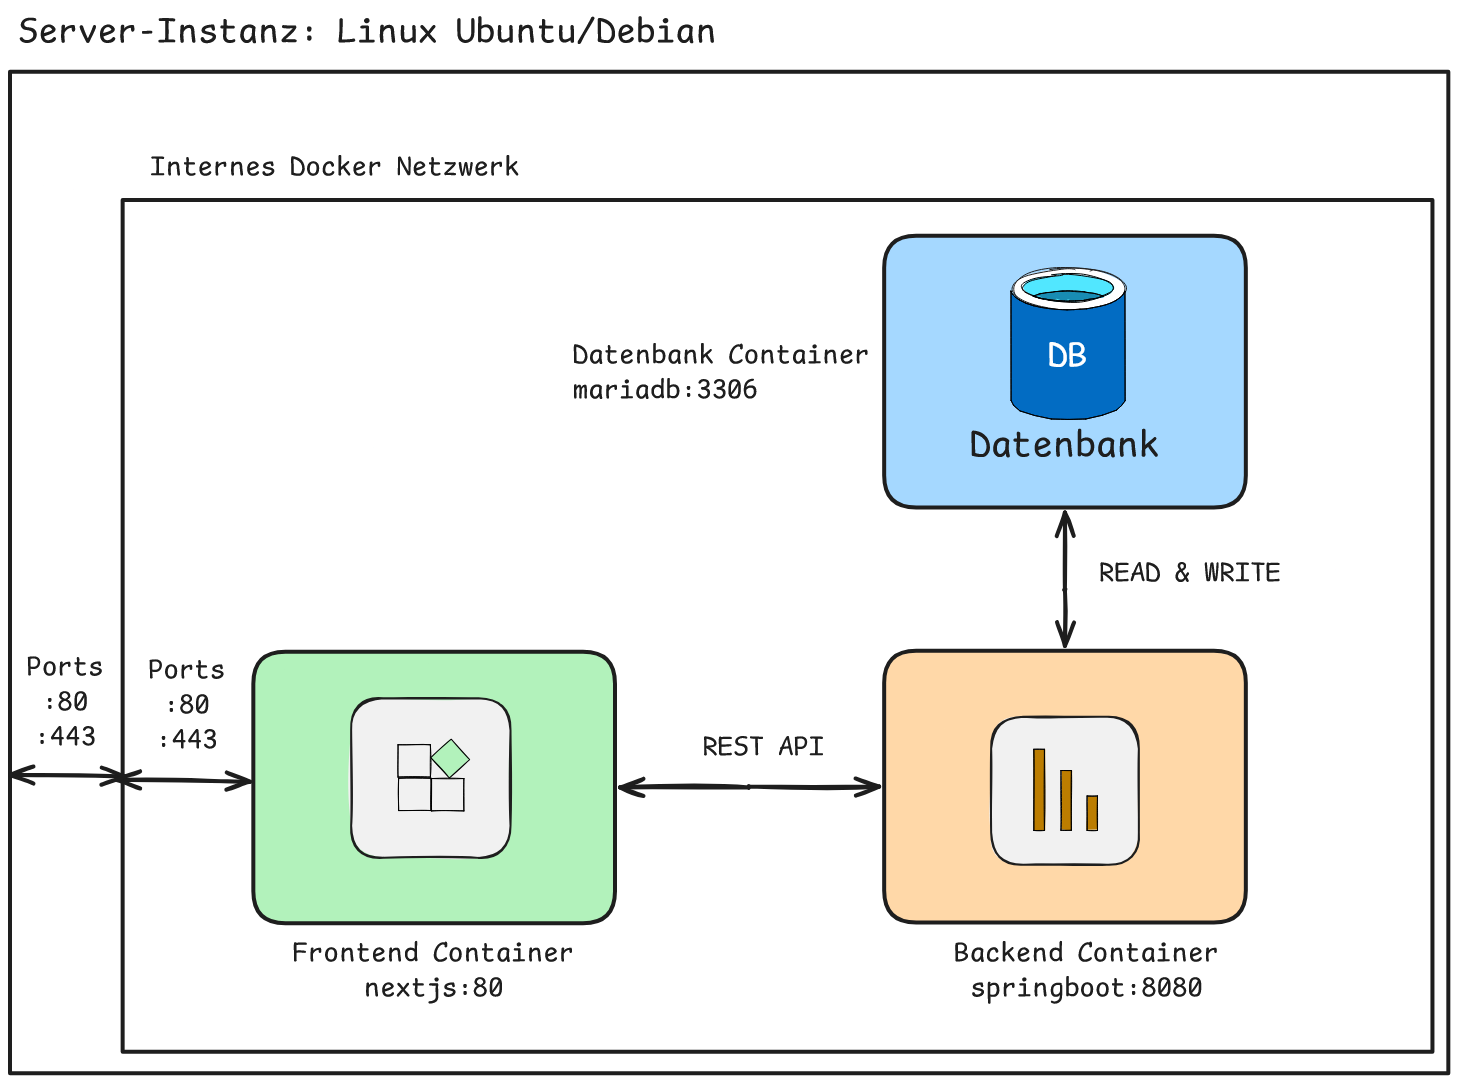
\includegraphics[width=0.9\textwidth]{images/architectural-design.png}
	\caption{Grafische Darstellung des Architekturdesigns. Es gibt hierbei genau 3 Komponenten, welche alle in einem internen Docker Netzwerk untergebracht sind. Darunter fallen das Frontend, das Backend und die Datenbank.}
    \label{koncept-archdesign-backend}
\end{figure}

Wie in Abbildung \ref{koncept-archdesign-backend} dargestellt, wird es drei Hauptkomponenten geben:

\begin{itemize}
	\item Das Frontend: Verantwortlich für die grafische Darstellung der Website und die Entgegennahme von Benutzerdaten.
	\item Das Backend: Verantwortlich für die Verarbeitung der vom Frontend empfangenen Daten und Kommunikation mit der Datenbank.
	\item Die Datenbank: Verantwortlich für die Speicherung aller Daten.
\end{itemize}

Die Applikation wird mit der Container-Technologie Docker \cite{website-docker} ausgeliefert, um den Build-Prozess zu vereinfachen.

\subsection{API-Design und Endpunkte}

Die API-Schnittstelle des Projekts wird mittels \textbf{REST} bereitgestellt, um eine effiziente Kommunikation zwischen Frontend und Backend zu gewährleisten. \textbf{Spring Boot} bietet dabei native Unterstützung für RESTful Web Services \cite{website-spring_rest}.

Folgende Endpunkte sind vorgesehen:
\begin{itemize}
	\item \textbf{POST /api/v1/forms}: Übermittlung eines Formulars vom Frontend an das Backend.
	\item 	\textbf{GET /api/v1/forms}: Anzeige aller gespeicherten Formulare.
	\item \textbf{GET /api/v1/forms/{id}}: Anzeige eines bestimmten Formulars.
	\item \textbf{PUT /api/v1/forms/{id}}: Aktualisierung eines bestehenden Formulars.
	\item \textbf{DELETE /api/v1/forms/{id}}: Löschen eines spezifischen Formulars.
\end{itemize}

Zur Sicherstellung der Datenqualität wird eine \textbf{Datenvalidierung} über die in Spring Boot integrierten Validierungs-Pakete vorgenommen. \textbf{Spring Security}\cite{website-spring_security} wird eingesetzt, um Authentifizierungs- und Autorisierungsfunktionen zu gewährleisten und den Zugriff auf die API-Endpunkte abzusichern.


\subsection{Workflow und Datenfluss}

Um sich jetzt ein konkretes Bild der Funktionalität der Applikation machen zu können, wird hier eine Beispielanfrage analysiert. 

Diese Anfrage soll sicherstellen, dass das Backend die Formulardaten vom Frontend korrekt verarbeitet und speichert.

\newpage

\subsection{Beispielanfrage des Frontends}

Es wurde bereits eine konkrete Datenstruktur entworfen, um diesen Prozess zu optimieren.

Der folgende Text, der im \gls{json}-Format ist, wird vom Frontend an das Backend an \textbf{POST /api/v1/forms} gesendet: \cite{website-git-backend-repo}

\begin{lstlisting}[language=Java, caption={Beispiel-Anfrage an das Backend.}]
...
"accommodation": 1,
"apartmentCountry": "ITALY",
"mainPerson": {
	"mainTraveler": true,
	"firstName": "Mario",
	"lastName": "Rossi",
	"gender": "MALE",
	"birthDate": "1985-04-12",
	"travelDocument": {
		"passportNr": "X12345678",
		"country": "ITALY",
		"issueDate": "2010-05-01",
		"issuing_authority": "Ministero dell'Interno"
...
\end{lstlisting}
		
		\subsection{Abarbeitung der Abfrage}
		
		\begin{figure}
			\centering
			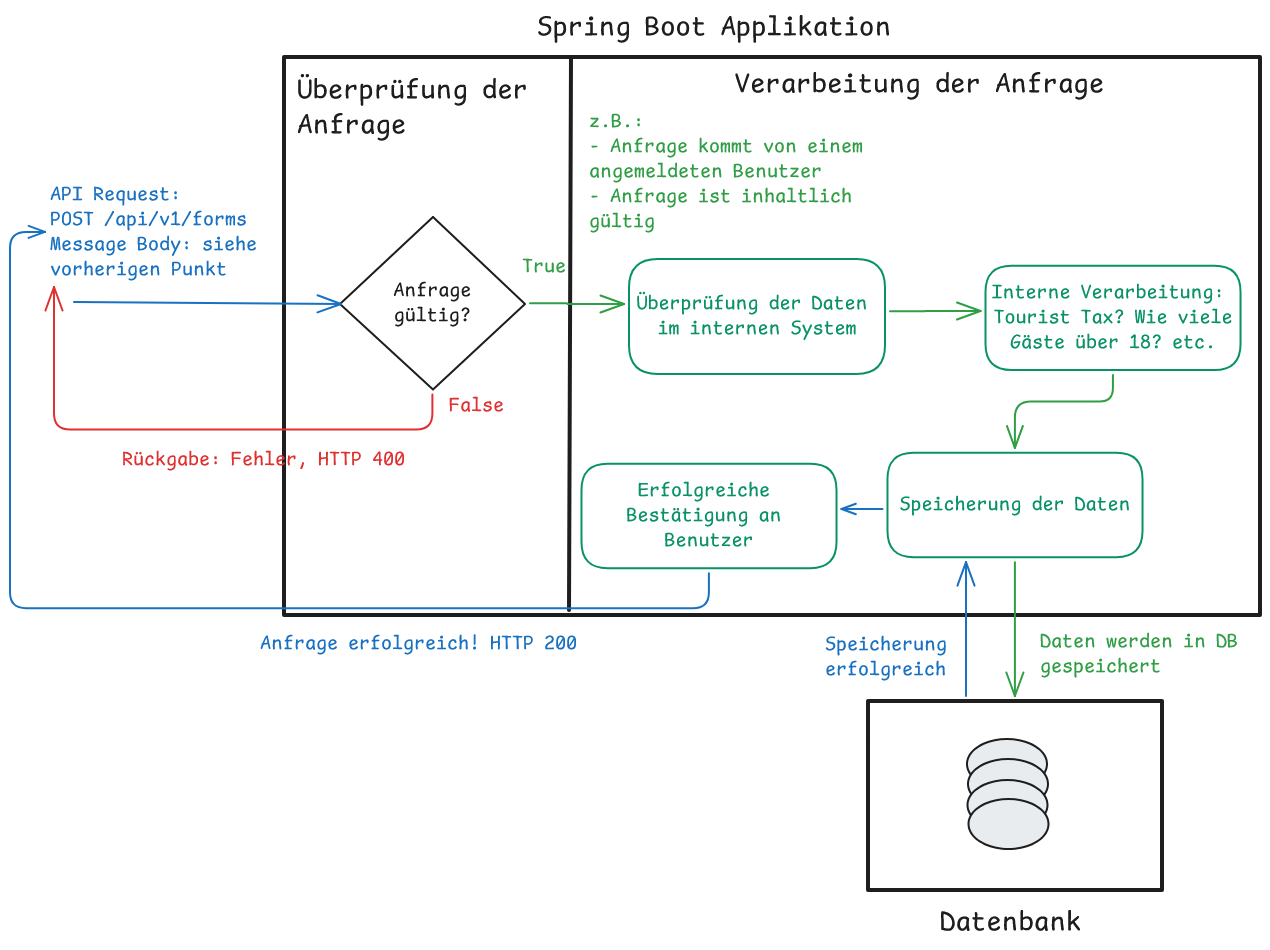
\includegraphics[width=0.9\textwidth]{images/Workflow-backend-post-form.png}
			\caption{Grafische Darstellung des Prozesses der Verarbeitung und Speicherung von Formulardaten im Backend.}
            \label{workflow-form-data-process-backend}
		\end{figure}
		
		Wie in Abbildung \ref{workflow-form-data-process-backend} dargestellt, läuft ein Prozess für die Verarbeitung und Speicherung von Formulardaten in etwa folgendermaßen ab:
		
		\begin{enumerate}
			\item Die Anfrage wird an den Endpunkt \textbf{POST /api/v1/forms} gesendet und auch empfangen.
			\item Die Anfrage wird auf ihre Gültigkeit überprüft: entsprechen die darin enthaltenen Daten der erwarteten Datenstruktur? Sind alle Informationen vorhanden? Falls dies nicht der Fall ist, bekommt der Benutzer einen Fehler angezeigt.
			\item Als Nächstes werden die Daten im internen System validiert. Dies bedeutet, dass z.B. überprüft wird, ob die Reisepassnummer des Hauptreisenden gültig ist, oder ob Daten wie Geburtsdaten usw. gültig sind.
			\item Anschließend werden die Daten intern von der Spring Boot Applikation verarbeitet: Die Objekte werden erstellt und Werte wie zum Beispiel, ob eine italienische Touristensteuer anfällt und wie viele Gäste volljährig sind, werden berechnet.
			\item Danach werden die Daten in die Datenbank eingepflegt. Falls dies erfolgreich gelungen ist, bekommt der Benutzer eine Bestätigung angezeigt.
		\end{enumerate}
\setauthor{Sebastian Sailer}
\section{Konzept zur Umsetzung der Datenbank}
\subsection{Einleitung}
Das Ziel dieses Konzepts ist die Bereitstellung eines Datenbanksystems (MariaDB) zur persistenten Speicherung der Daten und die Entwicklung eines Systems, welches Buchungsdaten aus der genannter Datenbank  exportieren kann. Es solle sowohl \textbf{CSV-} als auch \textbf{PDF-Dateien} bereitgestellt werden. Die Datenbankstruktur basiert auf dem ERD (Abbildung 7.3) und die Implementierung erfolgt wie der Rest des Backends mit \textbf{Java Spring} als Framework.


\vspace{3mm}
\makefig{images/ERD.png}{height=7cm}{ ERD }{fig:caption-label}



\noindent Das \gls{ac-erd}(siehe Abbildung 7.3) bildet die Grundlage für das relationale Schema in MariaDB. Es beschreibt, wie die einzelnen Tabellen miteinander verbunden sind. Die Tabellen sind normalisiert (\gls{3. Normalform}), um Redundanz zu minimieren und Datenintegrität sicherzustellen: 

\begin{itemize}
	\item \textbf{Primärschlüssel}: Jede Tabelle verfügt über einen eindeutigen Primärschlüssel
	\item \textbf{Fremdschlüssel}: Beziehungen zwischen Entitäten werden durch Fremdschlüssel abgebildet
	\item \textbf{Indexierung}: Häufig abgefragte Felder, wie \textit{checkIn} und \textit{accomadationid} werden indexiert, um die Abfragegeschwindigkeit zu erhöhen.
\end{itemize}

\subsection{Technologien und Bibliotheken}
Für die Umsetzung werden folgende Technologien und Bibliotheken verwendet:
\begin{itemize}
	\item \textbf{MariaDB:} Speicherung der Daten
	\item \textbf{Java Spring Framework:} Entwicklung des Backends.
	
\end{itemize}

\subsection{Architektur und Ablauf}
\subsubsection{Modularer Aufbau}
Das System wird in folgende Module aufgeteilt:
\begin{enumerate}
	\item \textbf{Datenbankmodul:} 
	\begin{itemize}
		\item Verbindung zur MariaDB-Datenbank
		\item Entitäten: \texttt{Booking}, \texttt{Person}, \texttt{Address}, \texttt{TravelDocument}, etc.
	\end{itemize}
	
	\item \textbf{Exportmodul:}
	\begin{itemize}
		\item CSV-Export: Generierung von CSV-Dokumenten
		\item PDF-Export: Generierung von PDF-Dokumenten
	\end{itemize}
	
	\item \textbf{API-Modul:} 
	\begin{itemize}
		\item Bereitstellung von Endpunkten für den Export (\texttt{/export/csv}, \texttt{/export/pdf}).
	\end{itemize}
\end{enumerate}

\newpage
\subsubsection{Ablaufdiagramm für den Export}
Die nachfolgenden Schritte beschreiben, das in Abbildung 7.4 dargestellte Ablaufdiagramm:
\begin{itemize}
	\item \textbf{Schritt 1:} Der Benutzer sendet eine Anfrage (HTTP GET) an die API mit den gewünschten Filterparametern (z. B. Zeitraum, Unterkunft, etc.).
	\item \textbf{Schritt 2:} Das Backend ruft die Daten aus der MariaDB-Datenbank ab.
	\item \textbf{Schritt 3:} Die Daten werden in das gewünschte Format (CSV oder PDF) umgewandelt.
	\item \textbf{Schritt 4:} Die generierte Datei wird dem Benutzer als Download bereitgestellt.
\end{itemize}

\makefig{images/Ablaufdiagramm.png}{height=15cm}{ Ablaufdiagramm des Exports }{fig:caption-label}



\subsection{Zusammenfassung}

Basierend auf der Nutzwertanalyse und den spezifischen Anforderungen des Projekts erweist sich \textbf{MariaDB} als die am besten geeignete Wahl (siehe Tabelle 6.4). Sie bietet eine hervorragende Balance zwischen Performance, Skalierbarkeit und Kosten, unterstützt durch die Vorteile einer großen Community und kostenfreier Verfügbarkeit. Während PostgreSQL besonders bei komplexen relationalen Abfragen überzeugt, ist MongoDB mit ihrer hohen Flexibilität und Skalierbarkeit auf unstrukturierte Daten spezialisiert – Eigenschaften, die in diesem Projekt jedoch nicht erforderlich sind. Amazon Aurora sticht durch exzellente Cloud-Integration und Zuverlässigkeit hervor, wurde jedoch aufgrund der hohen Kosten nicht priorisiert.

\vspace{2mm}

\noindent Die abschließende Bewertung durch die Nutzwertanalyse bestätigt \textbf{MariaDB} als die beste Wahl für dieses Projekt. Sie ermöglicht nicht nur eine solide und kosteneffiziente Lösung, sondern erfüllt die Anforderungen optimal, insbesondere im Hinblick auf die effiziente und \textbf{persistente} Speicherung von Buchungsdaten. Zudem unterstützt das Konzept den Export in \textbf{CSV-} und \textbf{PDF-Dateien}, wobei es flexibel und skalierbar genug ist, um zukünftige Erweiterungen wie zusätzliche Exportformate (z. B. Excel) oder Filteroptionen problemlos zu integrieren. (Prompt \cite{ChatGPT:rewrite4})
\setauthor{Sebastian Pollak}
\section{Konzept zur Umsetzung der Mieteransicht}
    \subsection{Einleitung}
    Folgend wird sich damit beschäftigt, wie das Produkt konkret umgesetzt werden kann. Aufbauend auf der Analyse der Anforderungen und den Ergebnissen der Machbarkeitsstudie wird ein detaillierter Plan zur Entwicklung des Systems vorgestellt. Ziel ist es, eine strukturierte Grundlage für die Entwicklung zu schaffen.
    
    \subsection{Zielsetzung}
    Die Entwicklung eines intuitiven und effizienten Formularsystems, das den manuellen Datenerfassungsprozess der equilibria GmbH automatisiert. Das System soll die Erhebung von Gästedaten gemäß den gesetzlichen Vorgaben in Österreich und Italien erleichtern und die Datenqualität durch Validierung und Vollständigkeitsprüfungen sicherstellen.
    
    \subsection{Anforderungen}

        \subsubsection{Funktionale Anforderungen}
        \begin{itemize}
            \item Bereitstellung länderspezifischer Eingabefelder für Österreich und Italien.
            \item Echtzeit-Validierung der Eingaben zur Sicherstellung der Datenintegrität.
            \item Überprüfung der Vollständigkeit der Daten vor dem Absenden.
            \item Integration mit dem Backend-System zur Datenübertragung
        \end{itemize}
        
        \subsubsection{Nicht-funktionale Anforderungen}
        \begin{itemize}
            \item Benutzerfreundliche und übersichtliche Gestaltung der Benutzeroberfläche.
            \item Einhaltung des firmeneigenen Stil der equilibria GmbH
            \item Sicherstellung der Datenvertraulichkeit und -sicherheit gemäß DSGVO.
        \end{itemize}

    \subsection{Technologischer Rahmen}
    \label{sec:technoglogischerRahmen}
    Basierend auf der Machbarkeitsstudie wurde entschieden, das von Mohamed Megahed ausgewählte Frontend-Framework mit dem von mir vorgeschlagenen zu kombinieren. Zum Einsatz kommen \gls{nextjs} und shadcn/ui in Verbindung mit React Hook Form. Für Validierungsschemata wird Zod verwendet, da dies, wie in der Dokumentation von shadcn/ui beschrieben, eine nahtlose Integration ermöglicht. \cite{prompt21_pollak}

    \subsection{Datenstruktur und Erfassung}
    Die Mieteransicht ist für die Erfassung der Gästedaten verantwortlich, wobei die erforderlichen Angaben je nach Land variieren. Die folgende Übersicht stellt die Unterschiede zwischen den in Österreich und Italien zu erfassenden Daten detailliert dar.
    
    \subsubsection{Erfasste Daten in Österreich}
    In Österreich müssen gemäß der Meldepflicht folgende Daten erfasst werden:
    \begin{itemize}
        \item \textbf{Persönliche Daten:} Familienname, Vorname, Geschlecht (Männlich, Weiblich, Divers), Geburtsdatum, Staatsangehörigkeit.
        \item \textbf{Reisedokument:} Reisepass oder Personalausweis mit Angabe von Ausstellungsdatum, ausstellender Behörde und Staat.
        \item \textbf{Adresse und Herkunftsland:} Straße/Gasse/Platz, Postleitzahl, Ortsgemeinde, Staat.
        \item \textbf{Mitreisende (falls vorhanden):} Name, Geburtsdatum.
        \item \textbf{Aufenthaltsdaten:} Datum der Ankunft, voraussichtliche Abreise und tatsächliche Abreise.
        \item \textbf{Tourist Tax:} Berechnung der anfallenden Abgaben.
    \end{itemize}
    
    \subsubsection{Erfasste Daten in Italien}
    In Italien ist eine manuelle Eingabe der Daten in das Portal der italienischen Polizei erforderlich. Erfasst werden:
    \begin{itemize}
        \item \textbf{Aufenthaltsdaten:} Anreisedatum, Anzahl der Nächte.
        \item \textbf{Herkunftsland und Staatsbürgerschaft.}
        \item \textbf{Falls Italiener:} Geburtsort.
        \item \textbf{Persönliche Daten:} Vorname, Nachname, Geburtsdatum (Format: DD/MM/YYYY).
        \item \textbf{Ausweisdokument:} Reisepass oder Personalausweis. Falls Reisepass: AIRE-Vermerk vorhanden?
        \item \textbf{Mitreisende:} Herkunftsland, Nachname, Vorname, Geburtsdatum, Geschlecht, Staatsangehörigkeit.
        \item \textbf{Tourist Tax:} Berechnung der anfallenden Abgaben.
    \end{itemize}
    
    Da viele dieser Daten unter die DSGVO-Kategorie "personenbezogene Daten" fallen und insbesondere die Reisedokumente als "sensible Daten" gelten, müssen sie unter strikter Einhaltung der Datenschutzrichtlinien verarbeitet werden.

\setauthor{Mohamed Megahed}
\section{Konzept zur Umsetzung der Mitarbeiteransicht}

\subsection{Architekturdesign}
Die Architektur in Next.js ist modular aufgebaut und verwendet wiederverwendbare Komponenten. Jede Komponente ist für einen spezifischen Bereich der Benutzeroberfläche zuständig, wie beispielsweise Header, Footer, Sidebar, Buchungsliste oder Filtermenüs. Dieser Ansatz ermöglicht eine bessere Organisation des Codes, erleichtert die Wartung und reduziert die Wahrscheinlichkeit von Fehlern. Durch die Trennung von Logik und Darstellung innerhalb jeder Komponente können Entwickler Änderungen schneller und sicherer vornehmen.\textit{\cite{rathinam2022analysis}}

\subsection{Datenfluss}
Die Kommunikation zwischen Frontend und Backend wird durch eine REST-API realisiert. Spring Boot, als Backend-Framework, bietet dabei eine native Unterstützung für die Erstellung und Verwaltung von RESTful Webservices. Dies ermöglicht eine flexible Datenübertragung und sorgt für eine klare Trennung zwischen Datenmanagement und Präsentationslogik. Mit dieser Architektur können beispielsweise Buchungsdaten effizient zwischen Frontend und Backend ausgetauscht und verarbeitet werden. \textit{\cite{shetty2020review, rathinam2022analysis}}

\subsection{Prototyping}

Mockups und interaktive Prototypen sind unverzichtbare Schritte im Entwicklungsprozess, um sicherzustellen, dass die geplante Anwendung den Anforderungen und Erwartungen der Nutzer entspricht. Sie legen den Grundstein für eine erfolgreiche Umsetzung und minimieren das Risiko von Fehlentwicklungen.


\subsubsection{Mockups}
Mockups dienen dazu, das endgültige Design vor der Entwicklung zu präsentieren. Sie ermöglichen Feedback und Freigaben, bevor Arbeit in die eigentliche Programmierung investiert wird. Die detaillierte Visualisierung hilft, Missverständnisse zwischen Designern, Entwicklern und Stakeholdern zu minimieren.

Programme wie Sketch, Figma oder Adobe XD werden häufig verwendet, um Mockups zu erstellen. Diese Tools bieten intuitive Funktionen, um präzise Designs zu erstellen und Designideen klar zu kommunizieren.

\newpage

\subsubsection{Interaktive Prototypen}
Der primäre Zweck interaktiver Prototypen liegt in der Durchführung von Usability-Tests, bei denen das Benutzerverhalten analysiert wird. Durch iteratives Feedback können Verbesserungen vorgenommen werden, bevor die eigentliche Entwicklung beginnt.
Programme wie InVision, Figma oder Axure RP ermöglichen die Erstellung von Prototypen mit realistischen Interaktionen.

\begin{figure}
	\centering
	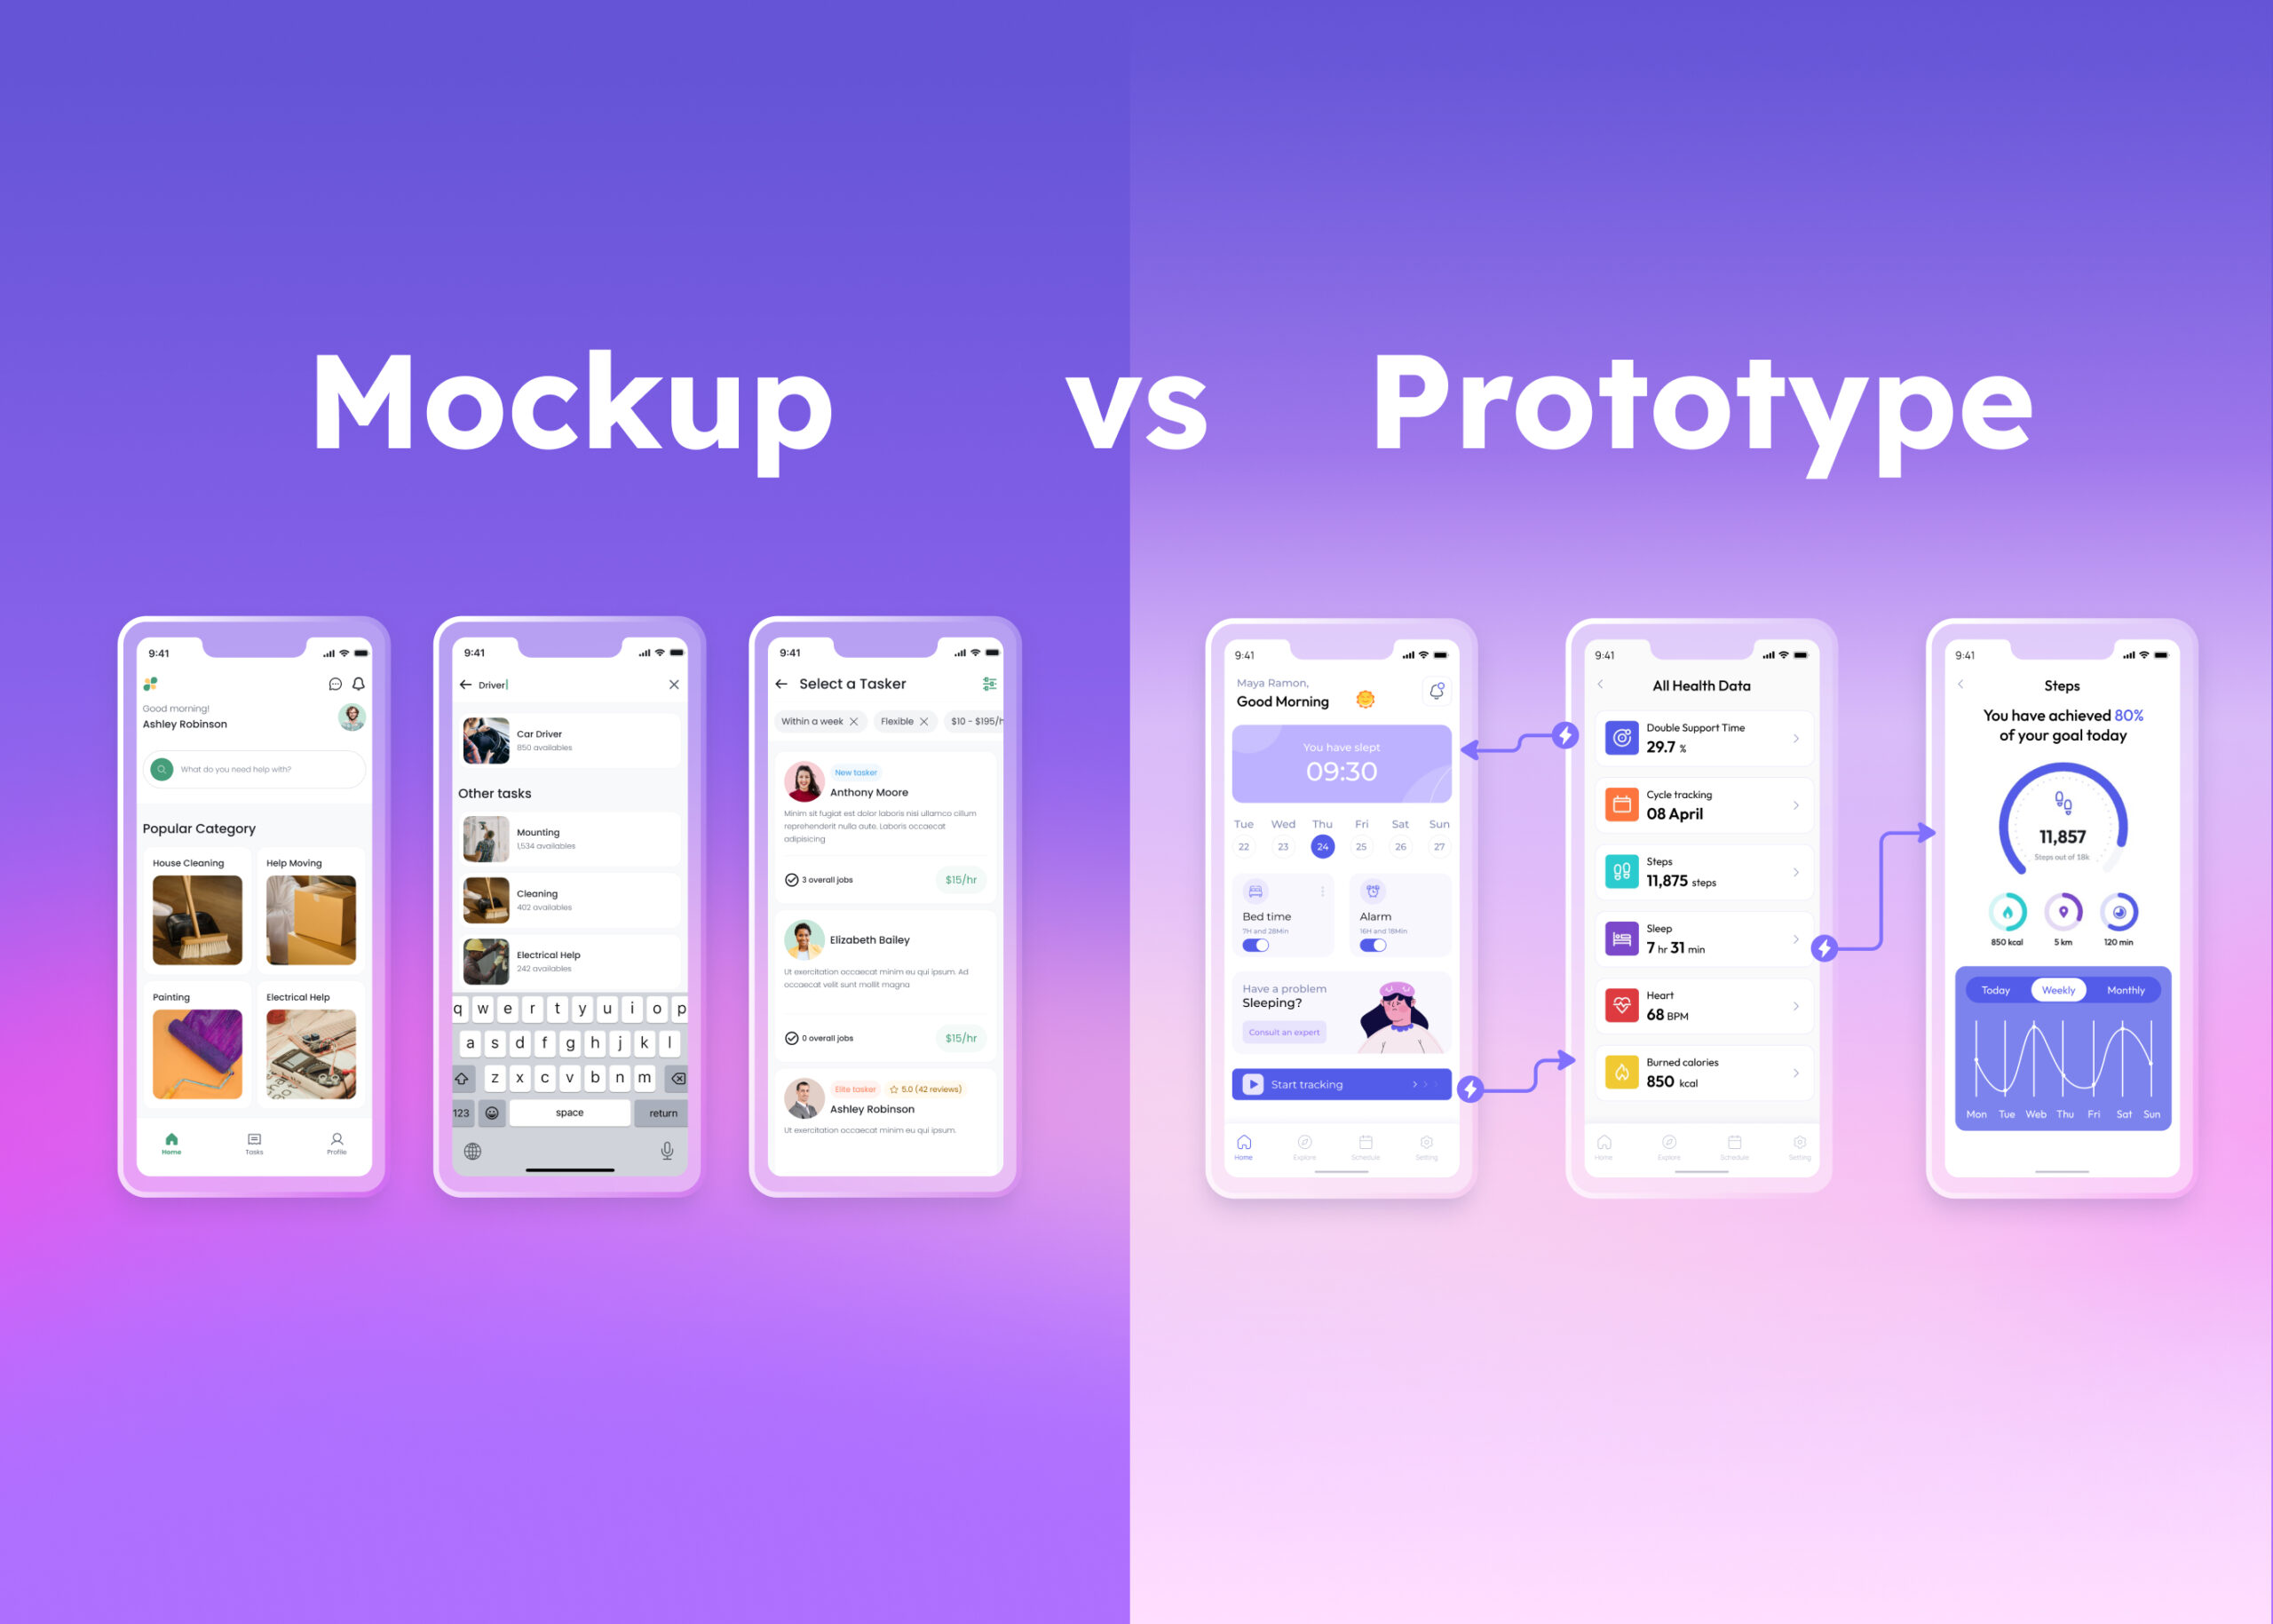
\includegraphics[width=0.75\textwidth]{images/Mockup-vs-Prototype.jpg}
	\caption{Mockup vs Prototype \textit{\cite{mockup_vs_prototype_image}}}
\end{figure}

\newpage

\subsection{Benutzeroberfläche (UI)}

\subsubsection{Struktur der Mitarbeiteransicht}

\textbf{Layout}
\begin{itemize}
	\item \textbf{Widget-basierte Darstellung:} Das Design bietet eine widget-basierte Darstellung, bei der wichtige Informationen in separaten, verschiebbaren und anpassbaren Widgets angezeigt werden. Dies ermöglicht eine flexible und personalisierte Nutzung der Benutzeroberfläche.
	\item \textbf{Responsive Design:} Das Layout passt sich automatisch verschiedenen Bildschirmgrößen an, um eine optimale Benutzererfahrung auf allen Geräten zu gewährleisten (z. B. Desktop, Tablet, Smartphone).
	
	\begin{figure}
		\centering
		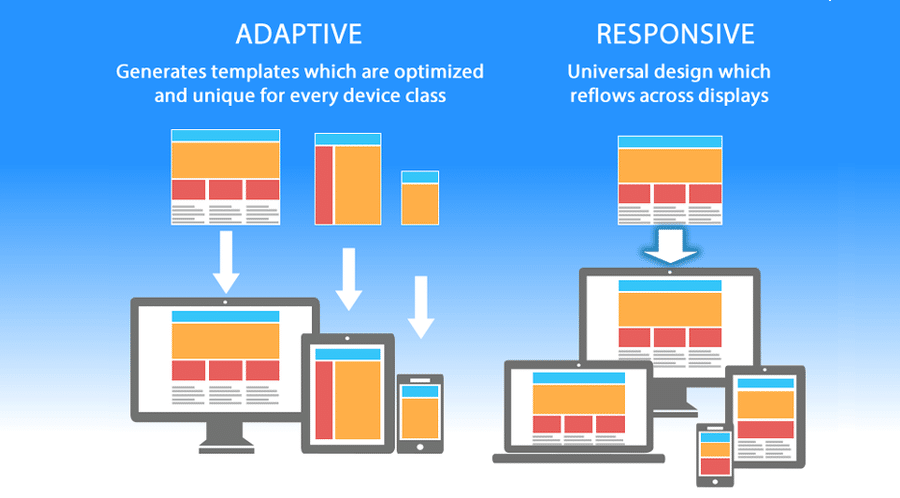
\includegraphics[width=0.75\textwidth]{images/responsive-vs-adaptive.png}
		\caption{Adaptives und responsives Layout\textit{\cite{responsive_vs_adaptive_image}}}
	\end{figure}
\end{itemize}


\subsubsection{Designprinzipien}

\textbf{Konsistenz}
\begin{itemize}
	\item \textbf{Einheitliche Farbpalette:} Primärfarben der Marke, unterstützt durch kontrastierende Akzentfarben. \textit{\cite{ux_usability}}
	\item \textbf{Schriftarten und UI-Komponenten:} Einheitliche Buttons, Dropdown-Menüs und Tooltip-Designs \textit{\cite{ux_usability}}
\end{itemize}

\textbf{Intuitive Bedienung}
\begin{itemize}
	\item \textbf{Eindeutige Beschriftungen:} Aktionen und Felder klar und prägnant benennen.
	\item \textbf{Kontextabhängige Tooltips:} Erklären Funktionen, ohne die Ansicht zu überladen.
	\item \textbf{Progressive Offenlegung:} Fortgeschrittene Optionen erst anzeigen, wenn der Benutzer sie benötigt.
\end{itemize}

\newpage

\subsection{Benutzerfreundlichkeit und Usability}

\textbf{Usability-Tests}
\begin{itemize}
	\item \textbf{Ziel:} Identifikation von Problemen und Ableitung von Verbesserungen für eine optimale Benutzererfahrung. \textit{\cite{ux_usability}}
	\item \textbf{Vorgehen:} 
	\begin{itemize}
		\item Beobachtungen und Analysen erfolgen, um Verbesserungsmöglichkeiten zu identifizieren. \textit{\cite{ux_usability}}
		\item Genutzte Methoden: Think-Aloud, First-Click-Tests und andere explorative Ansätze. \textit{\cite{ux_usability}}
	\end{itemize}
	\item \textbf{Nutzen:} Frühzeitiges Feedback zu Benutzerproblemen und Verbesserung der Benutzerfreundlichkeit. \textit{\cite{ux_usability}}
\end{itemize}


\textbf{Personas und Szenarien}
\begin{itemize}
	\item \textbf{Personas:} Stellt typische Benutzer mit spezifischen Zielen, Bedürfnissen und Herausforderungen dar. Zum Beispiel ein Büroangestellter, der regelmäßig mit Buchungssystemen arbeitet, benötigt intuitive Navigation. \textit{\cite{ux_usability}}
	\item \textbf{Szenarien:} Beschreiben realistische Nutzungssituationen, wie z. B.: „Ein Mitarbeiter möchte eine Buchung ändern und muss dafür die richtige Funktion finden.“ \textit{\cite{ux_usability}}
\end{itemize}

\textbf{Integration in den Entwicklungsprozess}

Durch den Einsatz agiler Methoden können nutzerzentrierte Tests und Feedbackzyklen effizient in den Entwicklungsprozess eingebunden werden. Prototypen und frühe Tests mit Endbenutzern helfen, potenzielle Probleme frühzeitig zu identifizieren und anzupassen.

% Dokumente für Implementierung

\chapter{Implementierung}

\setauthor{Manuel Fellner}
\section{Implementierung des Backends}

In diesem Kapitel wird die technische Umsetzung der Applikation beschrieben. Neben der Projektstruktur werden zentrale Komponenten der Implementierung, darunter das Backend, die API-Schnittstellen sowie Sicherheitsmaßnahmen, vorgestellt. Zudem werden Herausforderungen und Lösungsansätze erläutert.

\subsection{Projektstruktur und Überblick}

\subsubsection{Versionierungssoftware}

Für das Projekt wird das Versionierungssystem \texttt{git} verwendet. Dieses wird auf der Plattform namens Github (siehe \cite{website-github}) zur Verfügung gestellt und bietet damit eine optimale Entwicklungsumgebung. Für das Backend wurde ein separates \texttt{Repository} erstellt, welches unter folgender URL aufgerufen werden kann: \cite{website-git-backend-repo}. Alle Dateien, welche im Rahmen dieser Arbeit genauer untersucht und beschrieben werden, sind in diesem Repository auffindbar.

\subsubsection{Projektstruktur}

Das eigentliche Projekt unterteilt sich in die folgenden Hauptpakete:

\begin{itemize}
	\item \textbf{Controller}: Hier werden die Kontrollelemente der Applikation, damit unter anderem die REST-Schnittstellen programmiert.
	\item \textbf{Model}: In diesem Paket sind alle Datenstrukturen enthalten, welche für das Backend benötigt werden.
	\item \textbf{Repositories}: Hier befinden sich die jeweiligen Repositories zu den Model-Files, damit auf diese CRUD-Operationen (\gls{crud}) angewendet werden können (dies ist eine Funktionalität, welche von der \gls{jpa} zur Verfügung gestellt wird).
	\item \textbf{Config}: In diesem Ordner befinden sich applikationsübergreifende Konfigurationen, wie zum Beispiel die Security-Configuration für unsere REST API.
	\item \textbf{Services}: Hierbei handelt es sich um ein Paket, in dem Service-Elemente für die Authentifizierung zu finden sind.
	\item \textbf{Utilities}: Hier können nach Bedarf Dateien bzw. Programme eingefügt werden, die nicht mit den anderen Paketen kategorisierbar sind, jedoch trotzdem einen fixen Platz im Ablauf haben.
	\item \textbf{Exceptions}: Hier wird die eigene Implementierung der globalen Exception-Handling Struktur gespeichert.
\end{itemize}

\subsubsection{Einrichtung des Projekts}

Um das Projekt einzurichten, wurde der Spring Initializr (siehe \cite{website-spring-initializr}) verwendet. 

Die grafische Oberfläche dieses Werkzeugs sieht folgendermaßen aus:

\begin{figure}
	\centering
	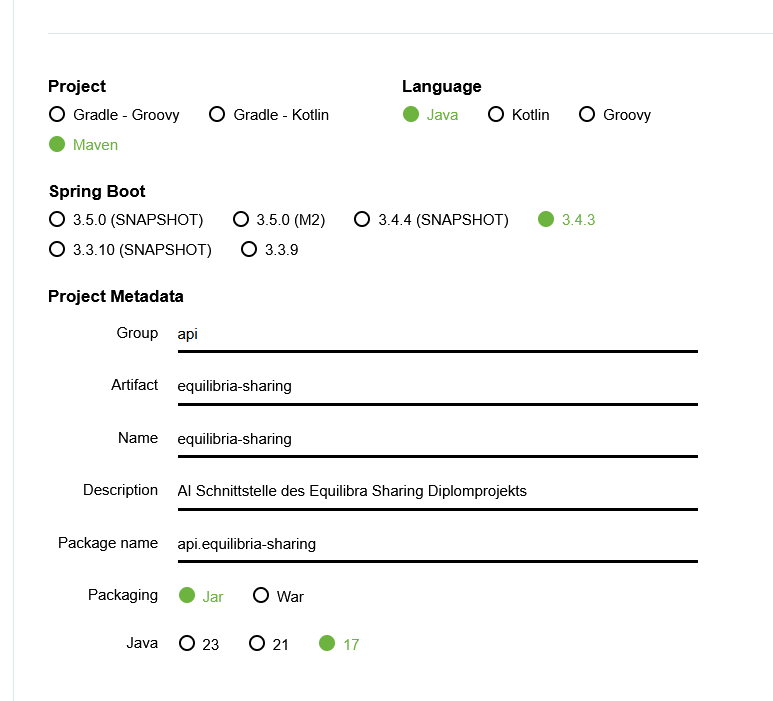
\includegraphics[width=1\textwidth]{images/impl-spring-init-1.png}
	\caption{Die grafische Darstellung des Spring Initializr. Hier werden allgemeine Projektdaten angegeben. \textit{\cite{website-spring-initializr}}}
    \label{backend-spring-init-1}
\end{figure}

In der Abbildung \ref{backend-spring-init-1} ist ein Teil der grafischen Oberfläche des Tools zu sehen. Hierbei können projektspezifische Daten, wie zum Beispiel der Name, die gewünschte Spring Boot Version, uvm. eingegeben werden.

\begin{figure}
	\centering
	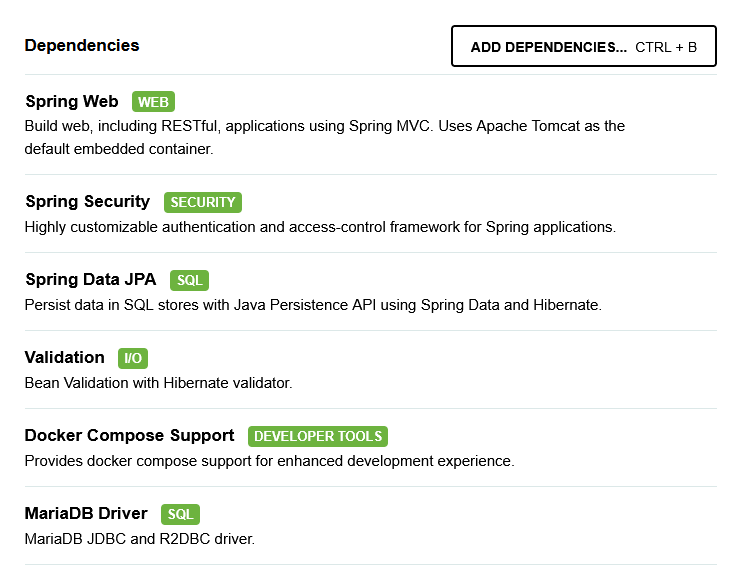
\includegraphics[width=1\textwidth]{images/impl-spring-init-2.png}
	\caption{Die grafische Darstellung des Spring Initializrs. In diesem Teil werden die gewünschten Pakete, welche im Projekt anfangs verwendet werden möchten, angegeben. \textit{\cite{website-spring-initializr}}}
    \label{backend-spring-init-2}
\end{figure}

Dieser Abbildung \ref{backend-spring-init-2} sind die jeweiligen Pakete, welche im Projekt anfangs verwendet wurden, zu entnehmen. Dabei können beliebige Pakete ausgewählt werden, welche bei der Generierung des Projekts automatisch eingebunden werden.

Nun wird ein ZIP-Archiv heruntergeladen, welches alle gewünschten Konfigurationen enthält. Dies bildet die Grundlage für das Equilibria Sharing Backend.

\subsection{API-Controller: Die Buchungsverwaltung}
\label{sec:apiDokumentation}
Die REST-Schnittstelle, welche die Verwaltung von Buchungen in der Anwendung bereitstellt, wird von dem sogenannten \texttt{BookingController} verwaltet. Hier befinden sich alle Endpunkte zum Erstellen, Abrufen, Aktualisieren und Löschen von Buchungen. Zudem sind Sicherheitsmechanismen zur Zugriffskontrolle implementiert. 

\subsubsection{Schnittstelle zur Datenbank}

Der Controller greift auf sogenannte \texttt{Repositories} zurück. Dies sind vorab definierte Interfaces, welche eine einfache Schnittstelle des Spring Boot Backends zur MariaDB-Datenbank ermöglichen. Damit lassen sich mittels Java-Quellcode Aktionen in der Datenbank ausführen.

Bei dieser API-Schnittstelle werden die folgenden Repositories verwendet:
\begin{itemize}
	\item \texttt{BookingRepository}: Verwaltung der Buchungseinträge
	\item \texttt{PersonRepository}: Speicherung der Reisenden
	\item \texttt{AccommodationRepository}: Verwaltung von Unterkünften
	\item \texttt{AddressRepository}: Speicherung von Adressen
\end{itemize}

Diese Repositories werden über den Konstruktor mithilfe der \gls{dependencyinjection} initialisiert (siehe \cite{website-spring-dependency-injection}):
\begin{lstlisting}[caption={Code-Ausschnit, welcher die Initalisierung aller notwendgen Klassen darstellt}, label={code-bookings-init}, language=Java]
	public BookingController(BookingRepository bookingRepository, 
	PersonRepository personRepository, 
	AccommodationRepository accommodationRepository,
	AddressRepository addressRepository) {
		this.bookingRepository = bookingRepository;
		[...]
	}
\end{lstlisting}

Damit werden direkt alle Schnittstellen zur Datenbank im Parameter des Konstruktors automatisch von Spring Boot mitgegeben und auch in die Klasse importiert.

Konkret müssen die Repositories jedoch noch folgendermaßen in der Klasse als Attribute hinterlegt sein:

\begin{lstlisting}[caption={Deklarierung der Repositories als finale (= nicht modifizierbare) Attribute.}, label={code-bookings-repositories}, language=Java]
	private final BookingRepository bookingRepository;
	private final PersonRepository personRepository;
	private final AccommodationRepository accommodationRepository;
	private final AddressRepository addressRepository;
\end{lstlisting}

Damit wird sichergestellt, dass die notwendigen Prozesse sorgfältig in der Datenbank abgearbeitet werden können.

\subsubsection{Erstellen einer Buchung}

Der Endpunkt \texttt{POST /api/v1/bookings} nimmt Buchungsanfragen entgegen. Die Methode \texttt{createBooking} validiert die Eingaben, speichert Hauptreisende, Adressen und Dokumente in der Datenbank und erstellt eine neue Buchung. Hierfür wird keine Authentifizierung benötigt, da die Aktion vom Benutzer ausgelöst wird. 

Bei dieser Anfrage ist die Angabe aller Buchungsdaten notwendig und im Normalfall auch vom Frontend gegeben. Dafür werden alle abgefragten Formulardaten in den Request Body gegeben, welcher dann in späteren Schritten extrahiert wird. Für eine detaillierte Übersicht über die benötigten Daten, siehe \cite{website-github-backend-example-booking-post}.

\newpage

\begin{lstlisting}[caption={Code-Ausschnitt des Buchungs-Controllers: Validierung der Eingaben bei der Erstellung einer neuen Buchung.}, label={code-bookings-userinput-body-validation}, language=Java]
	@PostMapping
	public ResponseEntity<Booking> createBooking(
	@RequestBody BookingRequest bookingRequest) {
		if (bookingRequest.getAccommodationId() == null || 
		bookingRequest.getMainTraveler() == null) {
			throw new BadRequestException();
		}
	\end{lstlisting}
	
	
	In dem obigen Codeblock \ref{code-bookings-userinput-body-validation} werden die Benutzereingaben aus dem Request Body extrahiert und erst einmal validiert, um fehlerhafte Anfragen zu verhindern.
	
	\begin{lstlisting}[caption={Erstellung des Personen-Objekts sowie setzen der mainTraveler Flag auf True.}, label={code-bookings-extract-main-traveler}, language=Java]
		Person mainTraveler = new Person();
		mainTraveler.setMainTraveler(true);
	\end{lstlisting}
	
	Hier wird der \enquote{Main Traveler}, umgangssprachlich der \enquote{Hauptreisende} initialisiert. Dafür wird eine Instanz der Klasse \texttt{Person} erstellt und das \texttt{mainTraveler} Attribut wird ebenso auf \texttt{True} gesetzt. Von dieser Person werden um einiges mehr persönliche Daten benötigt, welche im folgenden Schritt extrahiert werden:
	
	\begin{lstlisting}[caption={Extrahierung aller persönlichen Daten des Hauptreisenden.}, label={code-bookings-main-trav-extract-info}, language=Java]
		mainTraveler.setFirstName(bookingRequest.getMainTraveler()
		.getFirstName());
		mainTraveler.setLastName(bookingRequest.getMainTraveler()
		.getLastName());
		[...]
	\end{lstlisting}
	
	Wie in dem obigen Codeblock \ref{code-bookings-main-trav-extract-info} zu sehen ist, werden bei diesem Schritt die persönlichen Daten, wie z.B. der Vor- und Nachname, das Geburtsdatum usw. extrahiert und in der Personen-Instanz gespeichert.
	
	Der vorletzte Schritt bei der Erstellung einer neuen Buchung ist die Erhebung aller Mitreisenden. Von diesen Personen werden im Vergleich zum Hauptreisenden nicht so viele persönlichen Daten benötigt. Bei dieser Art von Reisenden sind es nur der Vor- und Nachname und das Geburtsdatum. Ebenso müssen diese Personen zu jeder Zeit einem Hauptreisenden zugeteilt sein.
	
	\begin{lstlisting}[caption={Erhebung aller Daten für jeden Hauptreisenden.}, label={code-bookings-other-travelers}, language=Java]
		Person person = new Person();
		person.setMainTraveler(false);
		person.setFirstName(guest.getFirstName());
		person.setLastName(guest.getLastName());
		person.setBirthDate(guest.getBirthDate());
		person.setMainTravelerRef(mainTraveler);
		personRepository.save(person);
	\end{lstlisting}
	
	Der Code-Ausschnitt \ref{code-bookings-other-travelers} stellt die Aktionen dar, welche für jeden einzelnen Mitreisenden durchgeführt werden. Es werden also die benötigten Daten extrahiert, die \texttt{mainTraveler} Flag wird auf \texttt{False} gesetzt und der Hauptreisende der Gruppe wird als Referenz angegeben.
	
	Das heißt, dass die Mitreisenden folgendermaßen vom Hauptreisenden unterschieden werden:
	
	\begin{enumerate}
		\item Persönliche Daten werden nicht im größerem Umfang gesammelt. Bei Mitreisenden ist dabei kein Reisedokument explizit erforderlich..
		\item In der Datenbank ist das \texttt{mainTraveler}-Attribut auf \texttt{False} gesetzt. Dies ermöglicht eine höchst effiziente Unterscheidung.
		\item Ebenso ist bei jedem Mitreisenden immer ein Hauptreisender als Referenz enthalten.
	\end{enumerate}
	
	Abschließend werden noch zwei wichtige Elemente berechnet:
	\begin{enumerate}
		\item \textbf{Tourist Tax}: Es wird berechnet, ob der Auftraggeber neben den normalen Nebenkosten noch zusätzlich für jeden Touristen eine extra Steuer bezahlen muss. Dies wird mittels \texttt{true} (also \texttt{wahr}) oder \texttt{false} (also \texttt{falsch}) gespeichert.
		\item \textbf{Personen über 18}: Es werden automatisch in der gesamten Reisegruppe alle Personen, welche am Check-in-Datum das 18. Lebensjahr vollendet haben, gezählt. Dies war zum einen der Wunsch des Auftraggebers und zum anderen ist dies ebenso von steuerlicher Relevanz. 
	\end{enumerate}
	
	\begin{lstlisting}[caption={Abschließende Berechnungen, relevant für administrative Tätigkeiten.}, label={code-bookings-tourist-tax}, language=Java]
		booking.calculateTouristTax();
		booking.calculatePeopleOver18();
		Booking savedBooking = bookingRepository.save(booking);
		return ResponseEntity.status(HttpStatus.CREATED).body(savedBooking);
	\end{lstlisting}
	
	Die praktische Ausführung der \texttt{calculateTouristTax()} und der \texttt{calculatePeopleOver18()} Methoden gestaltet sich einfach und effizient:
	
	\begin{itemize}
		\item \textbf{calculateTouristTax()}: Hier wird die angegebene Adresse des Hauptreisenden verwendet und überprüft, ob dieser aktuell seinen Wohnsitz in der gleichen Stadt wie die Unterkunft hat. Falls dies nicht so ist, wäre in Italien auf jeden Fall eine extra Steuer fällig.
		\item \textbf{calculatePeopleOver18()}: Diese Methode iteriert durch alle Personen der Reisegruppe und berechnet bei jeder das Alter in Jahren (ab dem Anreisetag). Hierbei wird ein Zähler bei jeder volljährigen Person um eins erhöht.
	\end{itemize}
	
	
	Am Ende wird die Buchung noch in der Datenbank gespeichert. Der Benutzer bekommt hierbei eine Kopie des gerade erstellten Objekts zurück.
	
	\textbf{Beispiel-Anfrage}: 
	
	Nun wird eine Buchung mit den folgenden Daten erstellt:
	
	\begin{itemize}
		\item Unterkunft mit der ID 1
		\item Hauptreisender: John, Doe, Männlich, geboren am 15.05.1985, in Besitz eines amerikanischen Reisepasses mit der Nummer \enquote{A1234567}
		\item Ist aktuell ansässig in Braunau am Inn
		\item Reist mit zwei Bekannten: Jane Doe (20.07.1988) und Mike Smith (30.10.1990)
		\item Check-in-Zeit: 01.02.2025 um 14:00
		\item Check-out-Zeit: 01.03.2025 um 17:30
	\end{itemize}
	
	Nun wird das alles in ein programmkonformes JSON-File eingetragen, in den Nachrichtenbody eingefügt und an \texttt{}{POST http://localhost:8080/api/v1/bookings} gesendet. Wir bekommen dabei die folgende Antwort:
	
	\begin{figure}
		\centering
		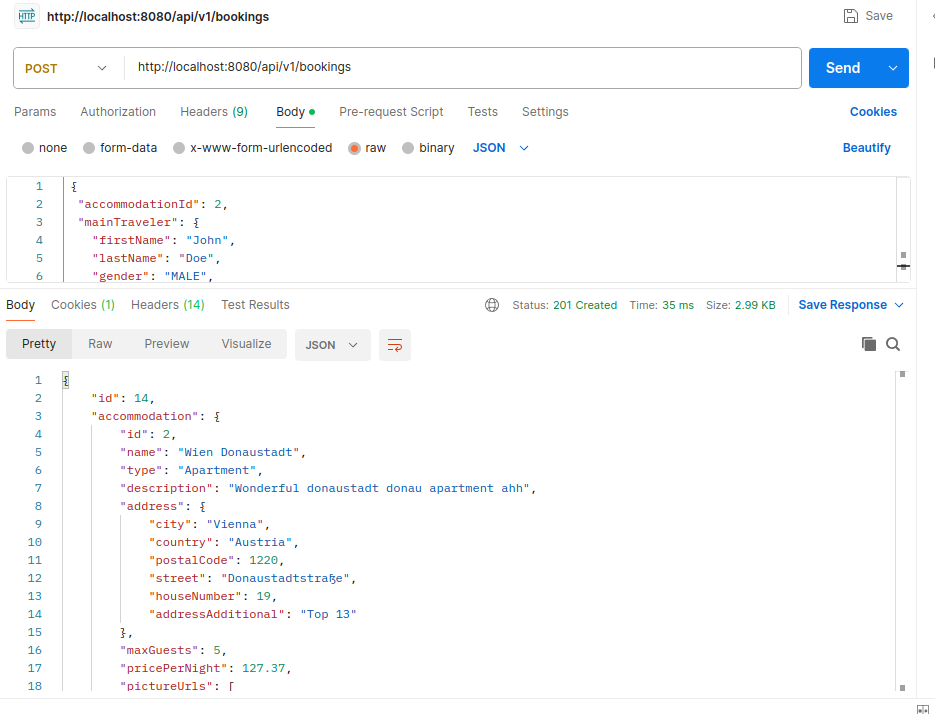
\includegraphics[width=1\textwidth]{images/impl-new-booking-post-req.png}
		\caption{Die Anfrage wurde erfolgreich abgeschickt und es wurde das gerade erstellte Objekt als JSON String zurückgegeben.}
        \label{req-bookings-post}
	\end{figure}
	
	Für das Testen der API-Schnittstellen wird Postman verwendet. Siehe \cite{website-postman}.
	
	Wie der Abbildung \ref{req-bookings-post} zu entnehmen ist, war die Anfrage erfolgreich. Wir haben den Status-Code 201 mit der Bedeutung \texttt{Created} zurückbekommen, das Objekt wurde also erfolgreich am Server erstellt und gespeichert.
	
	
	\subsubsection{Abrufen von Buchungen}
	
	Zum Abrufen von Buchungen wurden drei verschiedene Ansätze implementiert:
	\begin{enumerate}
		\item \textbf{getBookingById()}: Mit dieser Methode kann eine Buchung mit der exakten Buchungs-ID, welche in der Datenbank hinterlegt ist, abgerufen werden.
		\item \textbf{getAllBookings()}: Diese Methode ermöglicht das Abrufen aller gespeicherten Buchungseinträgen. Diese werden alle als JSON-String zurückgegeben.
		\item \textbf{getBookingsByAccommodation()}: Diese Methode wurde aufgrund des speziellen Use-Cases der Mitarbeiteransicht implementiert. Sie ermöglicht das Abrufen aller Buchungen, welche mit einer gewissen Unterkunft verknüpft sind. 
	\end{enumerate}
	
	Alle drei Ansätze haben etwas gemeinsam; sie lassen sich nicht einfach so im Internet aufrufen. Diese Methoden sind mittels Authentifizierung geschützt und es wird ein Mitarbeitertoken benötigt, um darauf zuzugreifen.
	
	\textbf{Abrufen einer Buchung mit der exakten Buchungs-ID}
	
	Der folgende Code-Ausschnitt repräsentiert die Logik hinter der Funktion, welche nur die Buchung mit der jeweiligen Buchungs-ID aufruft und zurückgibt:
	
	\begin{lstlisting}[caption={Aufrufen einer spezifischen Buchung mit der jeweiligen ID.}, label={code-bookings-get-booking}, language=Java]
		@PreAuthorize("isAuthenticated()")
		public ResponseEntity<Booking> getBookingById
		(@PathVariable("id") Long id) {
			Booking booking = bookingRepository.findById(id)
			.orElseThrow(() -> new ResourceNotFoundException());
			return ResponseEntity.ok(booking);
		}
	\end{lstlisting}
	
	In dem Code-Listing \ref{code-bookings-get-booking} wird als erstes sichergestellt, dass der Benutzer bzw. in diesem Fall der Mitarbeiter, der diese Buchung abrufen möchte, auch angemeldet ist. Wenn ein nicht angemeldeter Benutzer diese Schnittstelle aufruft, bekommt dieser einen \texttt{403-Fehler} (Forbidden). Die URL, um diese Methode aufzurufen, könnte lauten: \textit{https://example.com/api/v1/bookings/1}, wobei 1 für die ID des gewünschten Buchungs-Objektes steht. 
	
	\textbf{Abrufen aller Buchungen}
	
	Der folgende Codeblock \ref{code-bookings-get-all-bookings} zeigt die Funktionalität der Schnittstelle, alle gespeicherten Buchungen im JSON-Format auszugeben:
	
	\begin{lstlisting}[caption={Aufrufen aller in der Datenbank gespeicherten Buchungen.}, label={code-bookings-get-all-bookings}, language=Java]
		@PreAuthorize("isAuthenticated()")
		public ResponseEntity<List<Booking>> getAllBookings() {
			List<Booking> bookings = bookingRepository.findAll();
			return ResponseEntity.ok(bookings);
		\end{lstlisting}
		
		Dank dem \texttt{bookingRepository} ist das Laden aller Buchungen aus der Datenbank nur mit der \texttt{findAll()} Methode möglich. Dabei werden alle Buchungen in einer Liste vom Typ Booking gespeichert und dann zurückgegeben. Um diese Methode aufzurufen, genügt eine GET-Anfrage an die folgende URL: \newline
        \enquote{https://example.com/api/v1/bookings}.
		\newpage
		\textbf{Abrufen aller Buchungseinträge der jeweiligen Unterkunft}
		
		Nun gibt es auch noch die Möglichkeit, alle Buchungseinträge zu laden, welche an eine bestimmte Unterkunft geknüpft sind. 
		
		Dies wurde folgendermaßen implementiert:
		
		\begin{lstlisting}[caption={Aufrufen aller in der Datenbank gespeicherten Buchungen, welche mit der jeweiligen Unterkunft verknüpft sind.}, label={code-bookings-get-bookings-with-acc}, language=Java]
			Accommodation accommodation = accommodationRepository.findById(id)
			.orElseThrow(() -> new ResourceNotFoundException());
			List<Booking> bookings = bookingRepository
			.findByAccommodation(accommodation);
			return ResponseEntity.ok(bookings);
		\end{lstlisting}
		
		Der dargestellte Code im Listing \ref{code-bookings-get-bookings-with-acc} bekommt die ID der Unterkunft und durchsucht als Erstes die Datenbank danach, ob diese Unterkunft auch wirklich existiert. Falls nicht, wird ein \texttt{404-Error} geworfen.
		Als Nächstes werden dann alle Buchungs-Objekte aus der Datenbank gesucht, welche als Unterkunft (\texttt{Accommodation}) die übergebene und gefundene Unterkunft gesetzt haben.
		Das Abrufen dieser Methode lässt sich mit einer GET-Anfrage an die URL
		\enquote{https://example.com/api/v1/bookings/accommodation/1} bewerkstelligen, wobei 1 hierbei für die ID der Unterkunft stehen würde.
		
		\subsubsection{Beispiel-Anfrage: Abrufen aller Buchungen mit Unterkunft ID}
		
		Wir wollen uns nun alle Buchungen aus der Datenbank laden, welche im Zusammenhang mit der Unterkunft mit der ID = 2 stehen.
		
		Dafür muss folgendes vorhanden sein:
		
		\begin{enumerate}
			\item Der Benutzer muss angemeldet sein und einen gültigen Authentifizierungs-Token im Request Header übergeben.
			\item Die angegebene Unterkunft muss in der Datenbank existieren.
		\end{enumerate}
		
		\begin{figure}
			\centering
			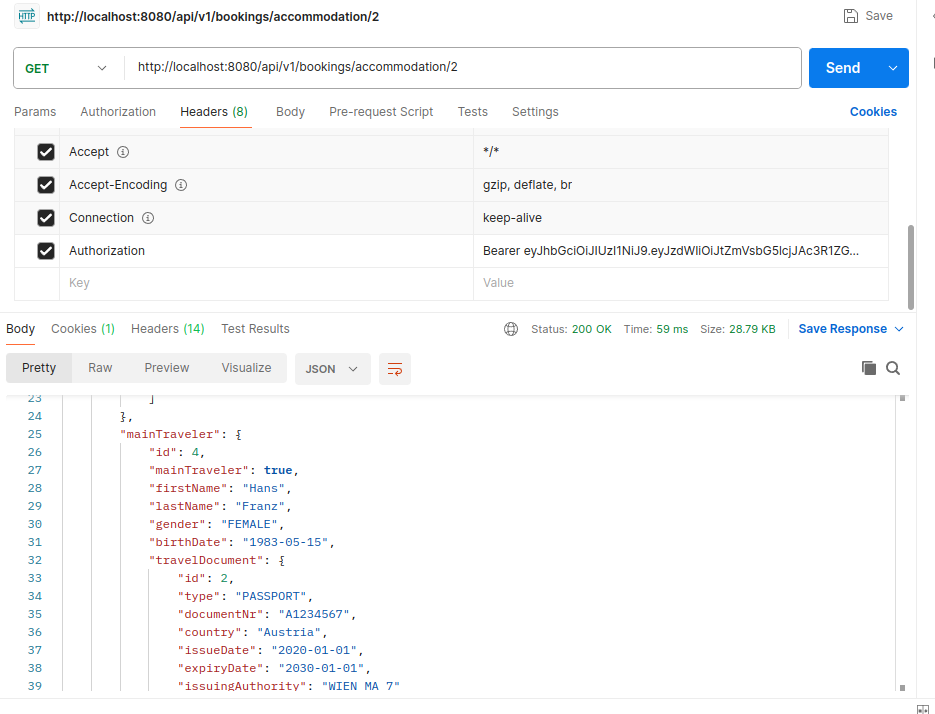
\includegraphics[width=1\textwidth]{images/impl-new-booking-get-acc-req.png}
			\caption{Die Anfrage wurde erfolgreich abgesendet und es wurden uns alle Buchungseinträge, welche mit der Unterkunft verknüpft sind, zurückgegeben.}
            \label{impl-new-booking-get-acc}
		\end{figure}
		
		Anhand der Abbildung \ref{impl-new-booking-get-acc} ist zu erkennen, dass die Anfrage erfolgreich war. Es wurden uns alle Buchungseinträge zurückgegeben, welche die Unterkunft mit der ID = 2 hinterlegt haben.
		
		\subsubsection{Aktualisieren und löschen von Buchungen}
		
		Die Operationen des Aktualisierens und Löschens der Buchungen basieren auf standardisierten Methoden, auf die nicht weiter eingegangen wird. Der vollständige Quellcode kann unter \cite{website-git-backend-repo} eingesehen werden.
		
		\subsection{API-Controller: Die Unterkunftsverwaltung}
		
		Neben der Buchungsverwaltung gibt es noch eine dedizierte Unterkunfts-Verwaltung, da diese einen essenziellen Teil im Workflow der Immobilienverwaltung von Equilibria darstellt. Dabei lassen sich neue Unterkünfte erstellen, abrufen, aktualisieren und löschen. Sicherheitstechnisch sind diese Schnittstellen weniger kritisch, da sie keine persönlichen oder sonstigen schützenswerten Daten beinhalten. Lediglich die Schreibvorgänge, also das Erstellen, Aktualisieren und das Löschen von Unterkünften, sind durch Authentifizierung geschützt. 
		
		\subsubsection{Erstellen einer Unterkunft}
		
		Um eine neue Unterkunft zu erstellen, werden die folgenden Daten benötigt:
		
		\begin{itemize}
			\item Name der Unterkunft
			\item Typ der Unterkunft (z.B. Haus, Wohnung, ...)
			\item Beschreibung
			\item Maximale Anzahl an gleichzeitigen Gästen
			\item Der Preis pro Nacht in €
			\item Die volle Adresse der Unterkunft
			\item (falls gewünscht) Eine Liste an Bild-URLS (kein direkter Image-Upload möglich)
		\end{itemize}
		
		Nun ist es möglich, als angemeldeter Mitarbeiter eine POST-Anfrage an die URL \break \enquote{https://example.com/api/v1/accommodations} mit den jeweiligen Daten zu machen. Für die vollständige Auflistung aller benötigten Daten siehe \cite{website-github-backend-example-accommodation-post}
		
		\begin{lstlisting}[caption={Überprüfung, ob die zu erstellende Unterkunft bereits in der Datebank existiert.}, label={code-acc-create-acc}, language=Java]
			@PostMapping
			@PreAuthorize("isAuthenticated()")
			public ResponseEntity<Accommodation> createAccommodation
			(@RequestBody AccommodationRequest accommodationRequest)  {
				if (accommodationRepository.findByName(accommodationRequest
				.getName()) != null) {
					throw new ConflictException();
				}
			\end{lstlisting}
			
			Als erstes wird hier in dem Listing \ref{code-acc-create-acc} überprüft, ob es bereits eine Unterkunft mit dem gleichen Namen in der Datenbank gibt. Falls dem so ist, wird eine sogenannte \texttt{ConflictException} (als ein Konflikt-Fehler) geworfen. Duplizierte Einträge können leicht vorkommen und Speicher und Performance negativ beeinflussen. Deshalb sind diese absolut zu vermeiden.
			
			\begin{lstlisting}[caption={Erstellung des Adress-Objektes für die Unterkunft}, label={code-acc-extract-info-out-of-body}, language=Java]
				Address address = new Address();
				address.setCity(accommodationRequest.getCity());
				[...]
				addressRepository.save(address);
			\end{lstlisting}
			
			Wie im Code-Listing \ref{code-acc-extract-info-out-of-body} zu sehen ist, werden im nächsten Schritt die Adressdaten aus dem Request Body extrahiert und in der Datenbank gespeichert.
			
			\begin{lstlisting}[caption={Erstellung eines neuen Accommodation-Objektes.}, label={code-acc-create-acc-objc}, language=Java]
			Accommodation accommodation = new Accommodation();
			accommodation.setAddress(address);
			accommodation.setName(accommodationRequest.getName());
			[...]
			accommodation.setPictureUrls(accommodationRequest.getPictureUrls());
			accommodationRepository.save(accommodation);
			return ResponseEntity.status(HttpStatus.CREATED).body(accommodation);
		\end{lstlisting}
		
		Dem Code-Listing \ref{code-acc-create-acc-objc} ist zu entnehmen, dass hier eine neue Instanz der Klasse Accommodation erstellt und initialisiert wird. Hier werden die zuvor erstellten und gespeicherten Adressdaten mit der Unterkunft assoziiert und sonstige Daten wie zum Beispiel die übergebenen Bild-Urls werden ebenso gesetzt.
		
		Schließlich wird die erstellte Unterkunft in der Datenbank gespeichert und es wird ein HTTP-Statuscode \texttt{200 - Created} inklusive dem gerade erstellten Objekt an den Client zurückgegeben.
		
		\subsubsection{Beispiel-Anfrage: Erstellung einer neuen Unterkunft}
		
		Wir möchten nun eine neue Unterkunft mit den folgenden Daten hinzufügen:
		
		\begin{itemize}
			\item Name: Villa Wien
			\item Type: Villa
			\item Beschreibung: Schöne Villa im 19. Wiener Gemeindebezirk
			\item Maximale Anzahl an gleichzeitigen Gästen: 20
			\item Preis pro Nacht: € 7849
			\item Adresse: Villastrasse 19, 1190 Wien, Österreich    
		\end{itemize}
		
		\begin{figure}
			\centering
			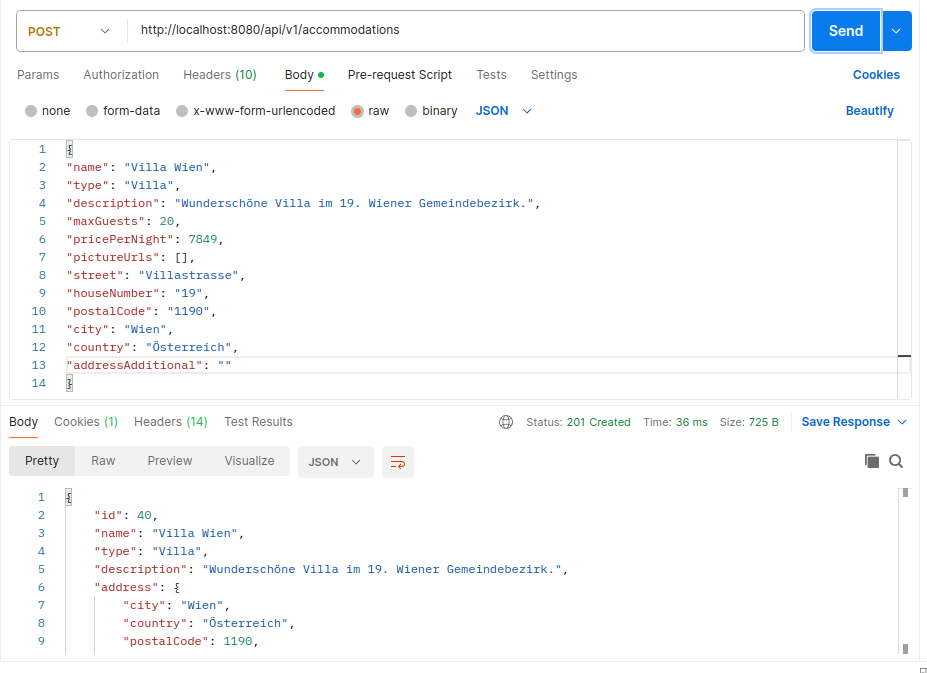
\includegraphics[width=1\textwidth]{images/impl-new-booking-post-acc-req.png}
			\caption{Die Anfrage wurde erfolgreich abgeschickt und es wurde uns der neu erstellte Accommodation-Eintrag zurückgegeben.}
            \label{impl-new-booking-post-acc-req}
		\end{figure}
		
		Wie in der Abbildung \ref{impl-new-booking-post-acc-req} zu sehen ist, war die Anfrage mit dem gesetzten Request Body erfolgreich. Das Accommodation-Objekt wurde erfolgreich erstellt und ist nun mit der ID = 40 in der Datenbank gespeichert. 
		
		\subsubsection{Abrufen, aktualisieren und löschen von Unterkünften}
		
		Die Operationen des Abrufens, Aktualisierens und Löschens der Unterkünfte basieren auf standardisierten Methoden, auf die nicht weiter eingegangen wird. Der vollständige Quellcode kann unter \cite{website-git-backend-repo} eingesehen werden.
		
		\subsection{Authentifizierung und Autorisierung}
		
		Die Implementierung der Authentifizierung und Autorisierung in dieser Anwendung basiert auf dem \gls{jwt} Standard. Dies ermöglicht eine sichere und effiziente Authentifizierung der Benutzer, insbesondere der Mitarbeiter des Auftraggebers, die Zugang zu geschützten Ressourcen benötigen. Anderenfalls wird dadurch unautorisierter Zugriff auf sensible Ressourcen vermieden.
		
		\subsubsection{JWT-Authentifizierung}
		
		Ein zentraler Bestandteil der Authentifizierung ist der \gls{jwt}, welcher nach erfolgreicher Anmeldung eines Benutzers generiert wird. Dieser Token wird für alle nachfolgenden Anfragen genutzt, um die Identität des Benutzers zu überprüfen. Die Logik für die Token-Verarbeitung ist in der Klasse \texttt{JwtService} implementiert. Siehe \cite{prompt-gpt-authentication-implementation}.
		
		\begin{lstlisting}[caption={Generierung eines JWT-Tokens für einen Benutzer.}, label={code-auth-create-jwt}, language=Java]
			public String generateToken(String username) {
				Map<String, Object> claims = new HashMap<>();
				return createToken(claims, username);
			}
		\end{lstlisting}
		
		
		Die Methode in \ref{code-auth-create-jwt} erzeugt ein JWT-Token mit dem übergebenen Benutzernamen und verwendet dabei eine Signatur, um die Integrität zu gewährleisten. 
		
		\begin{lstlisting}[caption={Validierung eines JWT-Tokens.}, label={code-auth-validate-jwt}, language=Java]
			public Boolean validateToken(String token, String username) {
				final String extractedUsername = extractUsername(token);
				return (extractedUsername.equals(username) && !isTokenExpired(token));
			}
		\end{lstlisting}
		
		Das Token wird bei jeder Anfrage an den Server überprüft, indem der Benutzername extrahiert und das Ablaufdatum validiert wird.
		
		\subsubsection{API-Controller: Registrierung}
		
		Die Registrierung eines neuen Mitarbeiters erfolgt über den Endpunkt \texttt{POST /api/v1/auth/register}. Dabei wird sichergestellt, dass nur autorisierte Personen neue Mitarbeiter registrieren können. Diese Funktionalität ist im \texttt{AuthController} vorhanden. Siehe \cite{prompt-gpt-authentication-implementation}.
		
		\begin{lstlisting}[caption={Validierung des Registrierungscodes bei der Anmeldung eines neuen Mitarbeiters.}, label={code-auth-employee-reg}, language=Java]
			if (!isValidUniqueCode(registerRequest.getUniqueCode())) {
				throw new BadRequestException("Invalid registration code provided");
			}
		\end{lstlisting}
		
		Dem Code-Listing \ref{code-auth-employee-reg} zu entnehmen ist der Anfang des Registrierungs-Prozesses. Als Erstes wird überprüft, ob der sogenannte \texttt{Unique Registration Code} korrekt ist. Dies ist ein Passwort, welches von der Firma lokal auf dem Server gesetzt wird. Nur mit diesem Passwort ist ein Registrierungsvorgang möglich.
		
		\begin{lstlisting}[caption={Erstellung eines neuen Mitarbeiter-Accounts.}, label={code-aut-employee-reg-2}, language=Java]
			Employee newEmployee = new Employee();
			newEmployee.setUsername(registerRequest.getUsername());
			newEmployee.setPassword(passwordEncoder.encode(registerRequest.getPassword()));
			newEmployee.addRole(Roles.EMPLOYEE);
			employeeRepository.save(newEmployee);
		\end{lstlisting}
		
		In dem Codeblock \ref{code-aut-employee-reg-2} wird ein neues Employee-Objekt mit dem gegebenen Benutzernamen und Passwort erstellt. Hierbei wird das Passwort mit der von Spring Boot Security bereitgestellten \texttt{PasswordEncoder.encode()} Methode gehasht und erst dann in die Datenbank gespeichert. Diese Speicherung stellt sicher, dass die Daten der Mitarbeiter nicht im Klartext in der Datenbank vorhanden sind – was ein enormes Sicherheitsrisiko wäre.
		
		Danach wird dem Mitarbeiter noch die \texttt{EMPLOYEE}-Rolle zugeteilt. Dies ist die Default-Rolle, welche alle Mitarbeiter des Auftraggebers bekommen. Ebenso wird im Code noch der zur Registrierung verwendete Unique Registration Code gespeichert, um mögliche Missbräuche des Codes sofort aufdecken zu können.
		
		\subsubsection{API-Controller: Login}
		
		Die Anmeldung erfolgt über den Endpunkt \texttt{POST /api/v1/auth/login}. Diese Funktionalität ist im \texttt{AuthController} vorhanden. Bei der Anmeldung muss ein valider Benutzername und ein valides Passwort eines existierenden Mitarbeiters angegeben werden. Siehe \cite{prompt-gpt-authentication-implementation}.
		
		\begin{lstlisting}[caption={Validierung der Benutzereingaben beim Login.}, label={code-auth-login-req}, language=Java]
			@PostMapping("/login")
			public ResponseEntity<?> login(@RequestBody LoginRequest loginRequest,
			HttpServletRequest request) {
				if (loginRequest.getUsername() == null || 
				loginRequest.getPassword() == null) {
					throw new BadRequestException();
				}
			\end{lstlisting}
			
			Hier, im Listing Nr. \ref{code-auth-login-req}, wird überprüft, ob die benötigten Daten angegeben wurden.
			Sofern ein Benutzername und Passwort angegeben wurden, wird der Mitarbeiter in der Datenbank gesucht und das Passwort überprüft.
			
			In dem folgenden Codeblock wird der Mitarbeiter aus der Datenbank geladen und es werden die Passwörter überprüft. Hierfür wird ebenso die von Spring Boot Security bereitgestellte \texttt{PasswortEncoder.matches()} Methode verwendet. Diese Methode ist kryptografisch sicher, da sie das gegebene Passwort hasht und diesen Hash dann mit dem gespeicherten Passwort-Hash in der Datenbank vergleicht. Somit kann im Programm das Passwort während des Vergleichs nicht extrahiert werden.
			
			\begin{lstlisting}[caption={Passwortprüfung und Token-Generierung bei erfolgreichem Login.}, label={code-auth-process-login-req}, language=Java]
				Employee employee = employeeRepository
				.findByUsername(loginRequest.getUsername());
				if (employee != null && passwordEncoder
				.matches(loginRequest.getPassword(), employee.getPassword())) {
					return ResponseEntity.ok().body(jwtService
					.generateToken(employee.getUsername()));
				}
				throw new BadRequestException("Invalid credentials were provided");
			\end{lstlisting}
			
			Falls das Passwort korrekt ist, wird eine HTTP-Request mit dem Status \texttt{200 - OK} mit dem JWT im Request Body zurückgegeben. Mit diesem Token kann der Mitarbeiter die geschützten Daten aus dem Backend abfragen. Dieser Prozess läuft automatisch im Frontend ab.
			
			\subsubsection{JWT-Filterung und Sicherheitsmechanismen}
			
			Um sicherzustellen, dass jede Anfrage authentifiziert ist, wird ein JWT-Filter genutzt, der die Tokens aus den Anfragen extrahiert und validiert. Siehe \cite{prompt-gpt-authentication-implementation}.
			
			\begin{lstlisting}[caption={Extrahierung des JWT-Tokens aus dem Authorization-Header.}, label={code-auth-jwt-service-extract-token}, language=Java]
				final String authHeader = request.getHeader("Authorization");
				if (authHeader == null || !authHeader.startsWith("Bearer ")) {
					filterChain.doFilter(request, response);
					return;
				}
			\end{lstlisting}
			
			
			Im Code-Listing Nr. \ref{code-auth-jwt-service-extract-token} wird der Code-Ausschnitt dargestellt, welcher überprüft, ob der Autorisationstoken im Request-Header enthalten ist. Dieser muss in der Form \texttt{Authorization: Bearer <token>} vorhanden sein, ansonsten wird die Anfrage sofort abgebrochen und es wird ein \texttt{403 - Forbidden} Status zurückgegeben.
			
			\begin{lstlisting}[caption={Validierung des JWT-Tokens und Setzen der Authentifizierung im Spring-Kontext.}, label={code-auth-jwtservice-validate-token}, language=Java]
				if (jwtService.validateToken(jwtToken, userDetails.getUsername())) {
					UsernamePasswordAuthenticationToken authToken =
					new UsernamePasswordAuthenticationToken(userDetails, null
					, userDetails.getAuthorities());
					SecurityContextHolder.getContext()
					.setAuthentication(authToken);
				}
			\end{lstlisting}
			
			Falls der Token, welcher übergeben wurde, gültig ist, wird die Benutzeridentität im Spring-Kontext gesetzt. Das heißt, dass die ganze Applikation nun weiß, wer dieser Benutzer ist. Es kann hiermit auch im gesamten Programm mit dieser Identität gearbeitet werden.

            \newpage
			
			\subsubsection{Spring-Security Konfigurationen}
			
			Zusätzlich zu den bis jetzt genannten Sicherheitsmaßnahmen werden ebenso Spring-Interne Sicherheitskonfigurationen gesetzt. Diese sind in der \texttt{SecurityConfig} enthalten.
			
			\begin{lstlisting}[caption={Initialisierung von allgemeinen Security-Konfigurationen wie dem Passwort-Encoder.}, label={code-spring-sec-conf-1}, language=Java]
				@Configuration
				@EnableWebSecurity
				public class SecurityConfig {
					@Autowired
					private JwtAuthenticationFilter jwtAuthenticationFilter;
					@Autowired
					private CustomUserDetailsService customUserDetailsService;
					@Bean
					public PasswordEncoder passwordEncoder() {
						return new BCryptPasswordEncoder();
					}
				\end{lstlisting}
				
				Das Code-Listing \ref{code-spring-sec-conf-1} stellt den Anfang der Security-Konfiguration von Spring Boot Security dar. Mittels \texttt{@Configuration} und \texttt{@EnableWebSecurity} deklarieren wir alles in dem File als Spring Konfiguration und aktivieren das Web-Security-Plugin.
				
				\begin{lstlisting}[caption={Erstellung der SecurityFilterChain in Spring Boot.}, label={code-spring-sec-conf-2}, language=Java]
					@Bean
					public SecurityFilterChain securityFilterChain(HttpSecurity http) {
						http.csrf(AbstractHttpConfigurer::disable)
						.cors(cors -> cors.configurationSource(corsConfigurationSource()))
						.authorizeHttpRequests(auth -> auth
						.requestMatchers("/api/v1/auth/login").permitAll()
						.requestMatchers("/api/v1/auth/register").permitAll()
					\end{lstlisting}
					
					In diesem Code-Listing Nr. \ref{code-spring-sec-conf-2} wird die sogenannte \texttt{SecurityFilterChain} in Spring Boot erstellt und zum Teil eingerichtet. Diese \enquote{Kette} ist für die Abarbeitung von Anfragen zuständig. Jede Anfrage, welche in den Server eingeht, muss als Erstes durch diese Filter-Chain gehen. 
					
					Wichtige Kriterien bei dieser Filter-Kette sind, dass:
					
					\begin{itemize}
						\item \gls{cors} ist aufgrund von Entwicklungsgründen noch aktiviert.
						\item \gls{csrf} ist aufgrund der hohen Sicherheitsrisiken deaktiviert. Siehe \cite{website-csrf-explanation}.
						\item Ebenso wurden explizit die zwei API-Pfade \texttt{/api/v1/auth/login} sowie \texttt{/api/v1/auth/register} freigegeben. Das bedeutet, dass jeder diese Endpunkte erreichen kann.
					\end{itemize}
					
					Da dies nur ein Teil der Konfiguration war, kommen wir nun zum restlichen Teil der Sicherheitskonfiguration:

                    \newpage
                    
					\begin{lstlisting}[caption={Fertigstellung der Definition der SecurityFilterChain in Spring Boot.}, label={code-spring-sec-conf-3},language=Java]
						.requestMatchers(HttpMethod.POST, "/api/v1/bookings")
						.permitAll()
						.requestMatchers(HttpMethod.GET, "/api/v1/accommodations")
						.permitAll()
						.requestMatchers(HttpMethod.GET, "/api/v1/accommodations/{id}")
						.permitAll()
						.anyRequest().authenticated()
						)
						http.addFilterBefore(jwtAuthenticationFilter, 
						UsernamePasswordAuthenticationFilter.class);
					}
				\end{lstlisting}
				
				In diesem Teil der Filter-Chain legen wir ebenso wichtige Konfigurationen fest:
				
				\begin{itemize}
					\item Die URL \texttt{/api/v1/bookings} darf nur als POST-Request unautorisiert erreicht werden. Dies dient dazu, damit sich der Mieter für das Ausfüllen des Formulars keinen extra Account oder Ähnliches erstellen muss.
					\item Ebenso dürfen die URLs \texttt{/api/v1/accommodations} sowie \texttt{/api/v1/accommodations/{id}} unautorisiert verwendet werden. Da diese Endpunkte keine Auskunft über sensible Informationen geben, ist dies sicherheitstechnisch auch unbedenklich.
					\item Danach wird durch \texttt{anyREquest().authenticated()} noch die Richtlinie gesetzt, dass jede Anfrage, welche nicht in das gerade genannte Muster passt, authentifiziert sein muss. 
					\item Schließlich wird durch \texttt{http.addFilterBefore()} noch unser vorher definierte JWT Authentication Filter hinzugefügt.
				\end{itemize}
				
				Diese Sicherheitsmaßnahmen sorgen für eine zuverlässige Authentifizierung und Autorisierung, indem sie sicherstellen, dass nur registrierte und berechtigte Benutzer auf geschützte Ressourcen zugreifen können.
				\subsection{Datenschutz und Sicherheit}
				
				\subsubsection{Speicherung und Schutz sensibler Daten}
				
				Zur Sicherheit und Nachverfolgbarkeit von Anmelde- und Zugriffsvorgängen werden die Klassen \texttt{AccessLogService} und \texttt{LoginLogService} genutzt. Diese speichern zum einen Anmeldungen aller Mitarbeiter inklusive UserAgent und IP-Adresse sowie relevante Zugriffe auf die API-Schnittstellen. Diese Einträge werden dann in der Datenbank archiviert.
				
				\subsubsection{Schutz personenbezogener Daten}
				
				Die Anwendung hält sich an die Datenschutz-Grundverordnung (DSGVO), indem personenbezogene Daten nur verschlüsselt gespeichert und verarbeitet werden. Sensible Informationen wie Passwörter werden mit einem sicheren Hashing-Algorithmus (BCrypt) gehasht, um unautorisierten Zugriff zu verhindern.
				
				\subsubsection{Zugriffskontrollen}
				
				Die Anwendung nutzt ein rollenbasiertes Zugriffskontrollsystem (RBAC), um sicherzustellen, dass nur autorisierte Benutzer bestimmte Aktionen durchführen können. Rollen wie \texttt{EMPLOYEE} und \texttt{ADMIN} definieren unterschiedliche Berechtigungen für die Nutzung der API-Endpunkte. Siehe \cite{prompt-gpt-datenschutz-implementation}.
				
				\subsection{Fehlerbehandlung}
				
				Es wurde eine eigene Exception-Handling-Struktur implementiert, um zu verhindern, dass dem Benutzer eventuell echte und ausschlaggebende Fehlermeldungen mit eventuellen Stacktraces angezeigt werden. Dies stellt ein großes Sicherheitsrisiko dar, da dem Benutzer in so einem Moment Einblick in das Innere der Applikation gewährt wird. Dadurch können eventuell sensible Daten ausgegeben werden. Diese Exception-Handling Struktur ist im \texttt{GlobalExceptionHandler} zu finden.
				
				\subsubsection{Globale Fehler}
				
				Globale Fehler in der Applikation, also Fehler, welche entweder nicht identifiziert werden konnten oder von externen Anbietern geworfen werden, werden als \enquote{generelle Exceptions} bezeichnet. Diese werden immer mit dem Status-Code \texttt{500 - Internal Server error} und der Fehlernachricht \enquote{An unexpected error occurred} ausgegeben. 
				
				Implementiert wird dieser Handler im Code folgendermaßen:
				
				\begin{lstlisting}[caption={Der Globale Fehler-Handler.}, label={code-global-exc-handler}, language=Java]
					@ExceptionHandler(Exception.class)
					public ResponseEntity<ErrorResponse> handleGeneralException(Exception ex) {
						ErrorResponse errorResponse = new ErrorResponse(
						LocalDateTime.now(), HttpStatus.INTERNAL_SERVER_ERROR.value(),
						"An unexpected error occurred."
						);
						return new ResponseEntity<>(errorResponse,
						HttpStatus.INTERNAL_SERVER_ERROR);
					}
				\end{lstlisting}
				
				Wie in dem Code-Listing Nr. \ref{code-global-exc-handler} zu sehen ist, werden hier alle globalen Fehler, welche nicht identifiziert oder sonst zugeordnet werden konnten, überarbeitet und ausgegeben. 
				
				\subsubsection{Applikationsspezifische Fehler}
				
				Neben den globalen Fehlern gibt es auch applikationsspezifische Fehler, welche die Usability verbessern sollen. 
				Darunter fallen die folgenden Exception-Klassen:
				
				\begin{itemize}
					\item \textbf{BadRequestException}: Wird geworfen, wenn der Server eine Anfrage bekommt, welche nicht alle für die weitere Verarbeitung notwendigen Parameter besitzt.
					\item \textbf{ConflictException}: Wird bei Datenbank-Duplikaten geworfen, da hier ein Konflikt entsteht.
					\item \textbf{ProtocolGenerationException}: Wird geworfen, wenn während der Generierung der Buchungsprotokolle fehler auftreten.
					\item \textbf{ResourceNotFoundException}: Wird geworfen, wenn eine angefragte Ressource auf dem Server nicht existiert.
					\item \textbf{UnauthorizedException}: Wird geworfen, wenn eine Ressource ohne die notwendige Authentifizierung aufgerufen wird.
				\end{itemize}
				
				\subsection{Zusammenfassung der Implementierung}
				
				\subsubsection{Reflexion der Herausforderungen}
				
				Während der Implementierung traten verschiedene Herausforderungen auf, insbesondere in den Bereichen Authentifizierung, Zugriffskontrolle und Fehlerbehandlung. Die korrekte Integration von Spring Security mit JWT stellte sich als komplizierter heraus, als ursprünglich gedacht, da unterschiedliche API-Endpunkte verschiedene Sicherheitsstufen benötigten.
				
				Ein weiteres Problem war das Exception Handling. Um sicherzustellen, dass Fehler nicht zu sensiblen Datenlecks führen, wurde ein \texttt{GlobalExceptionHandler} entwickelt, der kontrollierte Fehlermeldungen ausgibt und sicherheitskritische Details verbirgt.
				
				Schließlich war die größte Herausforderung das Paket-Management. Denn besonders hier ist es aufgrund von veralteten Versionen, verschobenen Paketen, uvm. oft zu Konflikten gekommen. Die Fehlernachrichten dieser Art von Fehlern waren sehr schwer zu interpretieren. Schließlich wurde eine einheitliche Struktur geschaffen, welche sich auch auf allen Betriebssystemen ausführen lässt. Siehe \cite{prompt-gpt-reflexion-implementation}.
				
				\subsubsection{Ausblick für mögliche Erweiterungen}
				
				Für zukünftige Versionen sind folgende Erweiterungen denkbar:
				
				\begin{itemize}
					\item \textbf{Feingranulare Zugriffskontrolle}: Detailliertere Implementierung des Role-Based Access Systems, um differenziertere Berechtigungsstrukturen zwischen den jeweiligen Rollen einführen zu können.
					\item \textbf{Erweiterte Protokollierung}: Ausbau der AccessLog- und LoginLog-Datenbank zur detaillierteren Analyse von Zugriffsmustern und Sicherheitsereignissen. Eventuell wäre hier eine automatische Auswertung der Zugriffe möglich, was den Sicherheitsfaktor noch einmal erhöht.
					\item \textbf{Caching-Struktur}: Die Implementierung einer Caching-Struktur würde die Performance der API besonders bei enorm großen Datenmengen um einiges erhöhen. 
					\item \textbf{Automatisierte Tests}: Ausbau von Unit- und Integrationstests zur Erhöhung der Stabilität und Reduzierung von Fehlerquellen in zukünftigen Versionen.
				\end{itemize} Siehe \cite{prompt-gpt-reflexion-implementation}.
\setauthor{Sebastian Sailer}
\section{Implementierung der Datenbank}
Alle relevanten Codeteile, sowie zusätzliche Dokumentationen sind im GitHub Repository verfügbar, das unter dem folgenden Verweis zugänglich ist: \cite{git:Eq}. In diesem Repository finden sich sowohl die Quellcodes für die Implementierung als auch ergänzende Dateien, die zur Dokumentation und zum besseren Verständnis des Projekts beitragen.

\subsection{Datenbankrealisierung}
\subsubsection{Erstellung der Datenbank}
Aufgrund der im Backend getroffenen Entscheidung für das Java-Framework \textit{Spring Boot} ging es bei der Implementierung des Projekts mehr um die Architektur, als die praktische Umsetzung der Datenbank. Während der konkreten Entwicklung des Projekts wurden zudem einige Optimierungsmöglichkeiten bemerkt und umgesetzt. Die eigentliche Erstellung der Datenbank erfolgt automatisch durch \gls{Docker} (weiteres dazu unter \hyperref[sec:deployment]{Deployment}). Die Tabellen werden anschließend durch Spring Boot und den geschriebenen Code automatisch generiert.

\begin{lstlisting}[language=Java, caption={Code-Ausschnitt: Erstellung einer Tabelle in der Datenbank.}]
@Entity
public class Person {
	@Id
	@GeneratedValue(strategy = GenerationType.IDENTITY)
	private Long id;
	@Enumerated(EnumType.STRING)
	private TravelDocumentType type;
	@ManyToOne
	private Address address;
			
\end{lstlisting}
	
	\noindent \textit{Baeldung} \cite{SB:Database} beschreibt, dass die Erstellung der Tabellen in Spring Boot automatisch durch Klassen erfolgt, die mit \textit{@Entity} gekennzeichnet sind. Der in Abbildung 8.26 dargestellte Code ist ein Beispielcode, der zur Veranschaulichung des Systems dient und in dieser Form nicht im Projekt enthalten ist. Der \textit{@Id}-Tag definiert den Primary-Key, welcher das erzeugte Objekt eindeutig identifizierbar macht. Der \textit{@ManyToOne} Tag zeigt an, dass eine Adresse mehreren Personen zugeordnet sein kann. Gleichzeitig dient er als Foreign-Key, was bedeutet, dass dieses Attribut eine eindeutige Referenz auf ein Objekt einer anderen Tabelle enthält.
	
	\newpage
	\subsubsection{Manipulation der Datenbank}
	\noindent Um nun der Datenbank einen neuen Eintrag hinzufügen zu können, verwendet Spring Boot das Spring Data JPA-Framework, welches das Arbeiten mit \gls{ac-CRUD} Operationen stark vereinfacht. Sogenannte Repositories sind Interfaces, mit denen sich Datenbankoperationen durchführen lassen, ohne dass man manuell SQL-Abfragen schreiben muss.
	
\begin{lstlisting}[language=Java, caption={Code-Ausschnitt: Repository.}]
@Repository
public interface BookingRepository extends
JpaRepository<Booking, Long> {
	List<Booking> findAllByCheckInBetween(LocalDateTime beginDate,
	LocalDateTime endDate);
}
			
\end{lstlisting}
	
	\noindent Abbildung 8.27 stellt das Repository dar, welches als Schnittstelle zwischen der Datenbank und dem Backend dient. Über dieses Repository erfolgen Interaktionen mit der Datenbank. Es gibt zwei Möglichkeiten, um mit der Datenbank zu kommunizieren. 
	
	\begin{enumerate}
		\item Durch Angabe des entsprechenden Methodennamens, wie im Beispiel in Abbildung 8.27 dargestellt.
		\item Alternativ kann ein Repository-Objekt erstellt werden, über das, wie in Abbildung 8.28 gezeigt, verschiedenste Methoden aufgerufen werden können.
	\end{enumerate}
	
	
\begin{lstlisting}[language=Java, caption={Code-Ausschnitt: Methoden-Aufrufe}]
personRepository.save(mainTraveler);
bookingRepository.findById(id)
bookingRepository.deleteById(id);
\end{lstlisting}
	
	\vspace{3mm}
	\noindent Damit ist es nun möglich, sämtliche vom Frontend übermittelten Daten direkt über den Code in der Datenbank zu speichern.
	
	\subsubsection{Datenbankstruktur}
	\makefig{images/uml.png}{height=10cm}{ERD der Datanbank des Projekts}{fig:caption-label}
	
	\noindent Im Gegensatz zu dem im Konzept erstelltem Diagramms wurden noch weitere Attribute hinzugefügt und die Namen vereinheitlicht. Jede dieser Kachel wird im Backend durch eine eigene Klasse repräsentiert. 
	
	
	
	\subsection{Buchungsprotokolle}
	\subsubsection{Controller}
	\noindent Der `ProtocolController` ist die zentrale Klasse zur Verarbeitung eingehender HTTP-Anfragen und zur Generierung von Protokollen in verschiedenen Formaten. Dabei ruft er relevante Buchungsdaten aus der Datenbank ab und verarbeitet sie entsprechend den Parametern der Anfrage.  
	
	\noindent Die Details einer Anfrage werden über die URL übermittelt. Ein Beispielaufruf könnte folgendermaßen aussehen:  
	
	\begin{center}
		\texttt{http://localhost:8080/api/v1/protocol?\textbf{format}=csv\&\textbf{accommodationID}=all\&\textbf{beginDate}=
			2025-01-01\&\textbf{endDate}=2025-02-28}
	\end{center}
	
	\noindent Die übergebenen Parameter aus dem Frontend bestimmen das Format, sowie die gewünschte Unterkunft und welche Datumsspanne das Protokoll abdecken soll.  
	\newpage
	\noindent \textbf{Parameter: accommodationID=} \vspace{3mm}\newline 
	\noindent Wie in Abbildung 8.29 dargestellt, kann über die \textbf{accommodationID} eine spezifische Unterkunft für das Protokoll ausgewählt werden.
	
\begin{lstlisting}[language=Java, caption={Code-Ausschnitt: Buchungen Laden mit Unterkunft.}]
bookingList = this.bookingRepository.findByDatumBetweenAndWert(
Integer.parseInt(accommodationID), beginDateTime, endDateTime);
\end{lstlisting}
	
	\noindent Falls jedoch \textbf{\enquote{all}} übergeben wird, werden alle Buchungen im angegebenen Zeitraum berücksichtigt. Hierfür wird die zweite, im Interface definierte, Methode aufgerufen, die alle Buchungen, welche den CheckIn Zeitraum zwischen den übergebenen Parametern hat, bereitstellt. Siehe dazu Abbildung 8.30.
	
\begin{lstlisting}[language=Java, caption={Code-Ausschnitt: Buchungen Laden.}]
if(accomodationID=="all"){
	bookingList = this.bookingRepository.findAllByCheckInBetween(
	beginDateTime, endDateTime);
}
\end{lstlisting}

	\vspace{3mm}
	\noindent \textbf{Parameter: format=}\vspace{3mm}\newline
	Zusätzlich dazu kann mithilfe des Format-Parametes angegeben werden, welches Dateiformat exportiert werden soll. Wobei zwischen folgenden 3 Dateitypen entschieden werden kann:
	
	\vspace{3mm}
	\begin{itemize}
		\item \textbf{PDF} – Generiert das Protokoll als PDF-Datei, ideal für den Druck oder die Archivierung.  
		\item \textbf{CSV} – Exportiert das Protokoll als CSV-Datei, welches einen strukturierten Überblick gibt.
		\item \textbf{XLSX} – Erstellt das Protokoll als Excel-Datei, optimal für strukturierte Datenanalysen.  
	\end{itemize}
	
	
	\vspace{3mm}
	\noindent \textbf{Parameter: beginDate \& endDate=}\vspace{3mm}\newline
	Diese beiden Parameter legen den Zeitraum fest, für den das Protokoll erstellt werden soll. Dabei wird das Ankunftsdatum verwendet, das sowohl in der Datenbank als auch im Code als \textit{LocalDateTime} gespeichert ist.
	
	\vspace{3mm}
	\noindent \textbf{Weiterverarbeitung}\vspace{3mm}\newline
	Mithilfe des ausgelesenen Formates und einem if-Statement werden dann die Daten, welche sich in der \textit{bookingList} befinden, an die entsprechende Methode weitergeleitet.
	\newpage
	\subsubsection{PDF}
	Um ein PDF mittels Java zu generieren, wird die 'itextpdf' Library verwendet. Um diese nutzen zu können, muss die benötigte Dependency in die \textit{pom.xml}-Datei hinzugefügt werden. Die Implementierung der Methode \textit{getPDF()} ist auf mehrere Methoden aufgeteilt, um nicht nur eine übersichtliche und gut formatierte PDF-Datei zu erzeugen, sondern auch den dafür benötigten Code so lesbar wie möglich zu machen.
	
	\vspace{3mm}
	\noindent Die Idee besteht darin, jede Buchung auf einer separaten Seite darzustellen. Dies verbessert die Lesbarkeit und Struktur des Dokuments. Das Erstellen des PDF-Dokuments selbst erfolgt direkt in der Methode \textit{getPDF()}, während die Gestaltung und Befüllung des Inhalts durch ausgelagerte Methoden realisiert wird. Dies fördert die Wartbarkeit, Wiederverwendbarkeit und Flexibilität des Codes.
	
	\vspace{3mm}
	In Abbildung 8.31 wird gezeigt wie das PDF zunächst erzeugt wird und anschließend in Querformat (Landscape-Modus) gesetzt wird:
	
\begin{lstlisting}[language=Java, caption={Code-Ausschnitt: PDF Dokument.}]
PdfDocument pdfDoc = new PdfDocument(writer);
Document document = new Document(pdfDoc);
pdfDoc.setDefaultPageSize(PageSize.A4.rotate());
\end{lstlisting}
	
	\noindent Danach wird die mitgegebene Liste von Buchungen \textit{(bookingList)} iteriert (durchgegangen). Für jede Buchung wird überprüft, ob ein Seitenumbruch erforderlich ist, um unnötige, leere, Seiten zu vermeiden. Dabei gilt:
	\begin{itemize}
		\item Die erste Buchung wird direkt auf die erste Seite geschrieben.
		\item Vor jeder weiteren Buchung wird ein Seitenumbruch eingefügt.
		\item Nach der letzten Buchung wird keine zusätzliche Seite mehr hinzugefügt.
	\end{itemize}
	
	\vspace{3mm}
	\noindent Die eigentliche Gestaltung jeder Buchungsseite erfolgt durch folgende drei Methoden:
	\begin{itemize}
		\item \textbf{addHeader()}: Erstellt die Überschrift und fügt sie dem Dokument hinzu.
		\item \textbf{addContentWithTables()}: Erstellt den Hauptinhalt der Buchung.
		\item \textbf{addBottom()}: Fügt die Fußnote auf jeder Seite hinzu.
	\end{itemize}
	
	\noindent Diese Aufteilung stellt sicher, dass der Code übersichtlich ist, modular bleibt und einzelne Abschnitte unabhängig voneinander geändert oder erweitert werden können. Durch den Einsatz von Methoden wird zudem eine übersichtliche Trennung der einzelnen Sektionen des PDFs erreicht.
	
	\vspace{3mm}
	\noindent Abschließend wird das Dokument geschlossen und zurückgegeben, sodass es heruntergeladen werden kann.
	
	
	
	\newpage
	\noindent \textbf{Methode: addHeader()}\vspace{3mm}\newline
	\noindent Die Methode \texttt{addHeader()} hat die Aufgabe, die Überschrift einer Seite zu erzeugen. Der Titel, der dabei verwendet wird, setzt sich aus den folgenden Informationen zusammen: \textit{"Buchung: Vorname Nachname - BookingID"}. Um eine klare visuelle Hierarchie zu schaffen, wird dieser Titel in einer größeren und fetteren Schrift dargestellt als der restliche Text. Zudem wird die Überschrift in eine Zelle einer Tabelle eingefügt, um die Platzierung der Elemente auf der Seite zu erleichtern. Am Ende der Methode wird die formatierte Überschrift dem Dokument hinzugefügt.
	
	\vspace{3mm}
	\noindent Der folgende Codeausschnitt zeigt, wie dies im Detail umgesetzt wird:
	
\begin{lstlisting}[language=Java, caption={Code-Ausschnitt: Header erstellen.}]
Cell titleCell = new Cell().add(titleParagraph);
headerTable.addCell(titleCell);
document.add(headerTable);
\end{lstlisting}

	\vspace{5mm}
	\noindent \textbf{Methode: addContentWithTables()}\vspace{3mm}
	
	\noindent Auch diese Methode teilt sich in unterschiedliche Aufgabenbereiche auf:
	
	\begin{enumerate}
		\item \textbf{table1} - Beinhaltet die allgemeinen Daten und das Bild
		\item \textbf{outertable / innertable} - Formatiert die allgemeinen Daten
		\item \textbf{tableDates} - Enthält die Datumsangaben der Buchung
		\item \textbf{tableAddOns} - Stellt die zusätzlichen Reisegäste dar
	\end{enumerate}
	
	\vspace{3mm} 
	
	\noindent Die Methode erstellt ein strukturiertes Dokument mit verschiedenen Tabellen, die die Buchungs- und Personendaten übersichtlich darstellen. Zunächst werden allgemeine Informationen über den Hauptreisenden, wie Name, Geburtsdatum und Reisedokument, formatiert und in einer Tabelle angeordnet. Anschließend folgen die Adressdaten sowie Details zum gebuchten Mietobjekt.  Ein Logo wird ebenfalls eingebunden, um das Dokument optisch abzurunden.  
	
	\vspace{3mm} 
	
	\noindent Daraufhin wird eine weitere Tabelle zur Darstellung der Buchungsdauer eingefügt, die Ankunfts- und Abreisedaten enthält. Schließlich listet die Methode in einer zusätzlichen Tabelle alle weiteren Reisenden auf, indem deren Namen und Geburtsdaten dargestellt werden. 
	
	
	\noindent Der in Abbildung 8.33 dargestellte Code Abschnitt zeigt, wie eine solche Tabelle erstellt wird, und wie mit Verschachtelung von Tabellen gearbeitet wird. Die letzte Zeile zeigt außerdem wie die Tabelle dem Dokument angehängt wird.
	
	
\begin{lstlisting}[language=Java, caption={Code-Ausschnitt: Verschachtelung.}]
Table innerTable = new Table(new float[] {2,1});
innerTable.setWidth(UnitValue.createPercentValue(100));
innerTable.addCell(creatCell("Vorname: Max"));
outerTable.addCell(new Cell().add(innerTable));
document.add(outerTable);
\end{lstlisting}
	
	\newpage
	\noindent \textbf{Methode: addBottom()}\vspace{3mm}\newline
	\noindent Die Methode \texttt{addBottom()} erstellt eine Fußzeile am unteren Rand jeder Seite des PDF-Dokuments. Sie enthält wichtige Informationen zu den Buchungen sowie den Namen der \textit{Equilibria Immobilienmanagement GmbH}.
	
	\vspace{3mm}
	\noindent Die Fußzeile wird in Form einer Tabelle mit drei Spalten realisiert:
	\begin{itemize}
		\item Die erste Spalte enthält eine Zusammenfassung der Buchungsdaten, einschließlich des frühesten Check-ins und des spätesten Check-outs.
		\item Die zweite Spalte bleibt leer, um visuell eine Trennung zwischen den Informationen zu schaffen.
		\item Die dritte Spalte enthält den Firmennamen „Equilibria Immobilienmanagement GmbH“ und wird rechtsbündig ausgerichtet.
	\end{itemize}
	
	\noindent Die Tabelle wird an einer festen Position am unteren Seitenrand platziert. Das Platzieren sowie die breite wird mithilfe der \texttt{setFixedPosition()} Methode angegeben. 
	
	\vspace{3mm}
	\noindent Der folgende Codeausschnitt zeigt, wie eine Fußzeile im Code umgesetzt werden könnte, mit verschiedensten Style-Attributen:
    
\begin{lstlisting}[language=Java, caption={Code-Ausschnitt: PDF-Footer.}]
Table unten = new Table(new float[]{1,2})
unten.addCell(new Cell().setWidth(100).setBorder(Border.NO_BORDER));
unten.addCell(createCell("test").setTextAlignment(TextAlignment.LEFT));
unten.setFixedPosition(36, 15, 500);
document.add(unten);
\end{lstlisting}
	
	\noindent \textit{Dieser Code Ausschnitt ist nur ein Beispiel-Code, welcher der einfachen Darstellung dient und wurde so nicht im Projekt verwendet.}
	
	\newpage
	\noindent \textbf{Exportiertes PDF}\vspace{3mm}\newline
	Dieses exportierte PDF ist mit Test-Daten ausgefüllt und dient lediglich der Darstellung der Ausgabe der vorher beschriebenen Methoden: 
	
	\makefig{images/pdf.png}{height=11cm}{ PDF Export }{fig:caption-label}
	
	
	\subsubsection{CSV}
    CSV steht für \textbf{C}omma-\textbf{S}eparated \textbf{V}alues. Dabei handelt es sich um eine Textdatei, in der Werte zeilenweise aufgeführt und durch Kommas getrennt sind. Tabellenkalkulationsprogramme wie Excel interpretieren diese Trennung oft so, dass die Werte in separate Zellen eingetragen werden, um die Lesbarkeit zu erhöhen. Die Tabellenüberschrift wird zunächst als String erstellt, in der die Spaltennamen durch Komma  getrennt sind. Danach werden die übergebenen Buchungsdaten zeilenweise im selben Format gespeichert. Der Output-String ist in Abbildung 8.35 dargestellt und erscheint im Vergleich zur formatierten Darstellung in Abbildung 8.8 unstrukturiert.
	
\begin{lstlisting}[language=Java, caption={Code-Ausschnitt: String Form eines CSV.}]
ID,Accommodation,MainPerson,CheckIn,ActualCheckOut,PersonsCount
123,Sea View Resort,John Doe,2025-01-20,2025-01-26,3
\end{lstlisting}

	\makefig{images/csv.png}{height=1cm}{ CSV Darstellung }{fig:caption-label}
	
	\noindent Um jede Buchung in eine eigene Zeile zu schreiben, wird am Ende jeder Buchung ein \textbf{\textbackslash n} angehängt, welches für einen Zeilenumbruch sorgt. Wurden alle Buchungen in den String eingefügt, wird er als Byte-Array im UTF-8-Format zurückgegeben, sodass er als Datei gespeichert werden kann.
	
	\subsubsection{Excel}
	Die Methode \texttt{getExcel} wird verwendet, um Buchungsdaten in eine Excel-Datei im \textbf{XLSX}-Format zu exportieren. 
	
	\noindent Zu Beginn wird ein \textit{Workbook} erstellt. Für den Export im \textbf{XLSX}-Format wird die \textit{XSSFWorkbook}-Klasse aus der \textbf{Apache POI}-Bibliothek verwendet, - "the Java API for Microsoft Documents". In dem Workbook wird ein Sheet mit dem Namen \textit{Buchung} erstellt, zu dem die Kopfreihe mit den benötigten Zellen erstellt wird.
	
	\noindent Anschließend wird wieder die übergebene \textit{BookingListe} durchgegangen und jede Buchung in eine Zeile gespeichert. Hierfür wird eine Zeile wie in Abbildung 8.36 erstellt und anschließend die Variable \textit{rowNum} erhöht, damit die nächste Buchung anschließend in eine neue Zeile geschrieben wird.
	
\begin{lstlisting}[language=Java, caption={Code-Ausschnitt: Reihe erstellen.}]
Row row = sheet.createRow(rowNum++);
\end{lstlisting}
    
	\noindent Danach werden alle Attribute des Buchungsobjekts so wie in Abbildung 8.37 dargestellt in die Zeile gespeichert. In welche Zelle dabei welches Attribut kommt, kann mit dem Index der \textit{createCell()} Methode angegeben werden. 

\begin{lstlisting}[language=Java, caption={Code-Ausschnitt: Zelle befüllen.}]
row.createCell(0).setCellValue(booking.getId());
\end{lstlisting}

	\noindent Abschließend wird der Output wieder in ein ByteArray gespeichert, um die Datei herunterladen zu können.
	
	
	
	
	
	\newpage
	\subsection{Deployment}
	\label{sec:deployment}
	\subsubsection{Erstellung eines Images mittels Docker}
	Um das Projekt schnell und einfach aufsetzen zu können, wurde entschieden, Docker zu verwenden. Docker ist eine \textbf{Containerisierungsplattform}, die es ermöglicht, Anwendungen mit ihren Abhängigkeiten in isolierten Containern auszuführen. Dadurch ist es irrelevant, auf welchem Betriebssystem gearbeitet wird.
	
	\vspace{3mm} \noindent
	Um ein sogenanntes Image auf den Docker Hub hochzuladen, muss man wie folgt vorgehen. Dabei ist es wichtig, einen Docker Hub Account zu besitzen und sich damit angemeldet zu haben.
	
	\begin{enumerate}
		\item Das gewünschte Projekt mittels \textit{mvn clean package} bauen, um eine ausführbare JAR-Datei zu erzeugen.
		\item Ein \texttt{Dockerfile} im Projektverzeichnis erstellen, das die Laufzeitumgebung definiert.
		\item In das Projekt-Verzeichnis wechseln
		\item Ein Docker-Image mit \textit{docker build -t bast1sa1ler/equilibria-sharing-backend:latest .} erstellen.
		\item Das Image mit \textit{docker push bast1sa1ler/equilibria-sharing-backend:latest} auf den Docker Hub hochladen.
	\end{enumerate}
	
	\noindent Mit diesen fünf Schritten kann das Projekt mithilfe eines passenden Dockerfiles auf Docker Hub veröffentlicht und zugänglich gemacht werden. Falls bereits kritische Daten vorhanden sind, sollten diese nicht veröffentlicht werden. Dies lässt sich durch eine `.dockerignore`-Datei verhindern, in der festgelegt wird, welche Dateien und Verzeichnisse nicht veröffentlicht werden sollen. 
	
	\subsubsection{Dockerfile}
	
	\begin{lstlisting}[language=Java, caption={Beispiel Dockerfile \cite{ChatGPT:docker}.}]
FROM openjdk:17-jdk-slim
WORKDIR /app
COPY target/equilibria-sharing-0.0.1-SNAPSHOT.jar /app/backend.jar
EXPOSE 8080
CMD ["java", "-jar", "/app/backend.jar"]
	\end{lstlisting}
	
	\noindent Das in Abbildung 8.38 gezeigte Dockerfile besteht aus fünf Zeilen. Die erste Zeile legt das Basis-Image fest. In diesem Fall eine Java-Laufzeitumgebung. Anschließend wird das Arbeitsverzeichnis im Container auf \texttt{/app} gesetzt, sodass alle nachfolgenden Befehle relativ zu diesem Verzeichnis ausgeführt werden.  
	
	\noindent Die dritte Zeile kopiert die erstellte JAR-Datei, welche im vorherigen Unterkapitel in Schritt 1 erstellt wurde, aus dem \texttt{target}-Ordner des Projekts in das \texttt{/app}-Verzeichnis des Containers und benennt sie in \texttt{backend.jar} um. Danach wird festgelegt, dass der Container den Port \texttt{8080} nutzt.
	
	\noindent Schließlich gibt die letzte Zeile den Befehl an, der beim Starten des Containers ausgeführt wird. In diesem Fall wird die JAR-Datei mit \texttt{java -jar} gestartet, um die Anwendung auszuführen.
	
	\newpage
	\subsubsection{Docker Compose}
	
	Docker Compose ist ein Tool, das es ermöglicht, mehrere Container-Anwendungen zu definieren und gemeinsam zu verwalten. Statt Container einzeln über die Kommandozeile zu starten, kann eine Datei verwendet werden, um alle benötigten Dienste, Netzwerke und Umgebungsvariablen in einer einzigen Datei zu deklarieren.
	
	\subsubsection{Erläuterung der Docker Compose Datei}
	
	Die Compose File ist in \textbf{4} verschiedene Sektionen eingeteilt. 
	\hyperref[sec:datenbank]{Datenbank}, \hyperref[sec:backend]{Backend}, \hyperref[sec:frontend]{Frontend} und die \hyperref[sec:netzwerk]{Netzwerk Konfiguration}. Sie dienen der Übersicht.
	
	\subsubsection{MariaDB-Service}
	\label{sec:datenbank}
	Der \texttt{mariadb}-Service basiert auf dem offiziellen MariaDB-Image:
	
	\begin{lstlisting}[language=Java]
image: 'mariadb:latest'
	\end{lstlisting}
	
	\noindent Es werden mehrere Umgebungsvariablen gesetzt, um die Datenbank zu konfigurieren:
	
	\begin{itemize}
		\item \texttt{MARIADB\_DATABASE=mydatabase} definiert den Namen der Datenbank.
		\item \texttt{MARIADB\_USER=myuser} gibt den Benutzernamen für die Verbindung an.
		\item \texttt{MARIADB\_PASSWORD=secret} und \texttt{MARIADB\_ROOT\_PASSWORD=verysecret} legen die Zugangsdaten fest. Diese sollten vor der Inbetriebnahme des Projekts geändert werden.
	\end{itemize}
	
	\noindent Der Standart-Port für MariaDB 3306 wird freigegeben und zusätzlich wird ein \texttt{healthcheck} durchgeführt, um zu überprüfen, ob die Datenbank erreichbar ist.
	
	\subsubsection{Backend-Service}
	\label{sec:backend}
	Das Backend basiert auf dem zuvor erstellten Docker-Image:
	
	\begin{lstlisting}[language=Java]
image: bast1sa1ler/equilibria-sharing_backend:latest
	\end{lstlisting}
	
	\noindent Es wird mit der Datenbank über Umgebungsvariablen konfiguriert:
	
	\begin{itemize}
		\item \texttt{DB\_HOST=mariadb} verweist auf den MariaDB-Container.
	\end{itemize}
	
	\noindent Weiteres werden die Daten übergeben, die benötigt werden um sich in der Datenbank anzumelden.
	
	\noindent Der Backend-Service hängt von der Datenbank ab:
	
	\begin{lstlisting}[language=Java]
depends_on:
	- mariadb
	\end{lstlisting}
	
	\noindent Dadurch wird sichergestellt, dass MariaDB vor dem Start des Backends hochgefahren wird. Zudem wird \texttt{restart: always} gesetzt, um den Container automatisch neu zu starten, falls ein Fehler auftritt.
	
	\subsubsection{Frontend-Service}
	\label{sec:frontend}
	Das Frontend verwendet das Image, welches im vorhinein auf den Docker-Hub gepusht wurde:
	
	\begin{lstlisting}[language=Java]
image: bast1sa1ler/equilibria-sharing_frontend:latest
	\end{lstlisting}
	
	\noindent Der Webserver ist über Port 3000 erreichbar:
	
	\begin{lstlisting}[language=Java]
ports:
	- '3000:3000'
	\end{lstlisting}
	
	\subsubsection{Netzwerk-Konfiguration}
	\label{sec:netzwerk}
	Alle drei Dienste sind über ein gemeinsames Netzwerk verbunden:
	
	\begin{lstlisting}
networks:
	mynetwork:
    	driver: bridge
	\end{lstlisting}
	
	Dadurch können die Container untereinander über ihre Servicenamen kommunizieren.
	
	\subsubsection{Fazit}
	Die Docker-Compose-Datei übernimmt die Koordination der drei Container, um eine reibungslose Kommunikation zu gewährleisten. Alle notwendigen Konfigurationen sind in einer einzigen Datei hinterlegt, die mit nur einem einzigen Befehl ausgeführt werden kann:
	
	\begin{lstlisting}[language=Java]
docker-compose up -d
	\end{lstlisting}
	
	\noindent Dies vereinfacht die Bereitstellung und Verwaltung der Anwendung erheblich. Möchte man den Code ändern, muss das veränderte Image erneut veröffentlicht und die Docker-Compose-Datei erneut ausgeführt werden.
	
	\newpage
	\subsection{Zusammenfassung \& Reflexion}
	Während der Implementierung traten verschiedene Herausforderungen auf, insbesondere in den 
	Bereichen der gestaltung des PDFs mittels iText, aber auch kleine Probleme bei dem Docker-Deployment.
	
	\vspace{3mm}
	\noindent Die, wie erwartet, größte Herausforderung stellte die Generierung und Strukturierung eines PDFs mit iText da. 
	Die präzise Anordnung der Inhalte von Tabellen und Bildern, 
	erforderten eine detaillierte Anpassung der Layout-Parameter und ein durchdachtes System der Verschachtelung. Da sich Objekte von Zeit zu Zeit nicht so verhielten wie gedacht, nahm dieser Teil des Projektes viel Zeit in Anspruch. 
	
	\vspace{3mm}
	\noindent Im Großen und Ganzen gab es jedoch keine großen Komplikationen, welche dem Projektfortschritt im Wege standen.
	

\setauthor{Sebastian Pollak}
\section{Implementierung des Formularsystems}

\subsection{Überblick}
Alle relevanten Codeteile sowie ergänzende Dokumentationen sind im GitHub-Repository verfügbar, das unter dem folgenden Link eingesehen werden kann: \cite{equilibriaSharingFrontend}. In diesem Repository sind sowohl die Quellcodes der Implementierung als auch zusätzliche Dateien enthalten, die zur Dokumentation und zum besseren Verständnis des Projekts beitragen.

\subsection{Verwendete Technologien und Pakete}
\label{sec:verwendeteTechnologien}
Im Rahmen der Machbarkeitsstudie wurde ein technischer Rahmen definiert, an den sich die Implementierung des Projekts gehalten hat. Wie in \ref{sec:technoglogischerRahmen} beschrieben, wurden für das Frontend Next.js 14.2.21 sowie shadcn/ui in Verbindung mit React Hook Form verwendet. Zur Definition von Validierungsschemata kam Zod zum Einsatz. Um die Webseite in mehreren Sprachen zur Verfügung zu stellen, wurde für die Internationalisierung die Bibliothek next-intl verwendet. 

\subsection{Projektstruktur}
Das Frontend wurde in zwei wesentliche Teile gegliedert, die jedoch innerhalb eines einzigen Projekts umgesetzt wurden. Diese Gliederung umfasst die Mitarbeiteransicht sowie die Mieteransicht. Im Folgenden wird erläutert, wie diese Struktur im Next.js-Projekt konkret umgesetzt wurde.

\subsubsection{Umsetzung}
In der verwendeten Version von Next.js existiert ein ``src``-Verzeichnis, das die zentrale Projektstruktur organisiert. Innerhalb dieses Verzeichnisses befindet sich der ``app``-Ordner, welcher sämtliche Seiten des Projekts enthält. Die Erreichbarkeit dieser Seiten erfolgt über die Namensgebung der jeweiligen Unterordner, wodurch das \gls{routing} in Next.js automatisch gesteuert wird.

Zusätzlich sind alle wiederverwendbaren \gls{components} des Projekts im components-Verzeichnis abgelegt. Die Struktur wurde so gestaltet, dass sowohl der ``app``- als auch der ``components``-Ordner eine logische Unterteilung für die beiden Hauptbereiche des Frontends aufweisen. Dies sorgt für eine klare Trennung der Funktionalitäten und erleichtert die Wartung sowie Erweiterbarkeit des Codes. \cite{prompt23_pollak}

Die hierarchische Struktur der Projektorganisation wird in der folgenden Darstellung verdeutlicht:

\dirtree{%
	.1 src.
	.2 app.
	.3 (other).
	.3 tenantDataManagement.
	.3 tenantRegistration.
	.2 components.
	.3 tenantDataManagementComponents.
	.3 tenantRegistrationComponents.
	.3 ui.
}

Wie in der Darstellung zu sehen, enthält der ``components``-Ordner auch einen Unterordner namens ``(other)``, der Seiten enthält, die keiner der beiden Hauptansichten zugeordnet werden können. Dazu gehören beispielsweise Fehlerseiten oder rechtliche Seiten. Die Klammern um den Namen dieses Ordners dienen dazu, dass dieser nicht als Pfad im Browser berücksichtigt wird. Der Ordner dient ausschließlich der Strukturierung und Organisation des Codes.

Zusätzlich gibt es einen Ordner namens ``ui`` im ``components``-Verzeichnis, der die \gls{components} aus shadcn/ui enthält. Alle anderen Komponenten, die für beide Ansichten des Frontends verwendet werden, sind direkt im ``components``-Ordner abgelegt.

\subsection{Frontend-Entwicklung des Formularsystems}
\subsection{Komponentenstruktur und Aufbau}
Das Formularsystem besteht gemäß dem Lastenheft aus zwei Formularen, die die erforderlichen Daten unter Berücksichtigung der rechtlichen Anforderungen der jeweiligen Länder erfassen. In diesem Fall handelt es sich um die Länder Österreich und Italien. Es wurden zwei \gls{components} entwickelt, die sich lediglich in den erfassten Daten unterscheiden, um den länderspezifischen Anforderungen gerecht zu werden.
Die Seite tenantRegistration entscheidet anhand der Adresse des Apartments, welches der beiden Formulare angezeigt werden muss. Auf die genauere Umsetzung dieser Formulare wird im weiteren Verlauf eingegangen, jedoch wird zunächst eine allgemeine Einführung in den Aufbau von \gls{components} benötigt.\cite{prompt24_pollak}

\subsubsection{Allgemeiner Aufbau von Komponenten}
\gls{components} in Next.js-Projekten folgen wie immer einem ähnlichen Schema. Dieses sieht folgendermaßen aus:

\begin{enumerate}
	
	\item \textbf{Importe} Zu Beginn müssen \gls{react} und andere benötigte Module importiert werden. Diese Importe können andere Komponenten, React-Funktionen oder zusätzliche Dateien wie CSS-Module umfassen.
\begin{lstlisting}[language=JavaScript]
import React from 'react';
import styles from './globals.css'; 
import { Input } from "@/components/ui/input";
	\end{lstlisting}
	
	\item \textbf{Komponenten-Funktion} Anschließend wird die Komponente definiert. Dabei werden ihr Name und die Parameter (Props) angegeben. Eine Next.js-Komponente kann entweder als export default function oder als benannte Funktion (export function) exportiert werden. Benannte Exporte ermöglichen es, mehrere Komponenten aus einer Datei zu exportieren.
\begin{lstlisting}[language=JavaScript]
export function ComponentName({ titel, description }) {
    ...
}
	\end{lstlisting}

\newpage

    
	\item \textbf{Layout} Das Layout wird mit \gls{jsx} geschrieben, einer Syntaxerweiterung für JavaScript, die HTML-ähnlichen Code ermöglicht. Hier können dynamische Werte mit Geschwungenden Klammern eingebunden werden. Der Rückgabewert (return) enthält den Code, das beim Rendern der Komponente ausgegeben wird.
\begin{lstlisting}[language=JavaScript]
return (
    <div>
    <h1>{title}</h1>
    <p>{description}</p>
    </div>
);
	\end{lstlisting}
	
	\item \textbf{Funktionen und Variablen} Das Layout kann mit JavaScript interagieren, um dynamische Inhalte zu ermöglichen. Dabei gibt es zwei Arten von Variablen:
	\begin{itemize}
		\item \textbf{Konstanten außerhalb der Komponente} Diese werden einmalig beim Laden des Moduls definiert und ändern sich nicht.
		\item \textbf{Variablen innerhalb der Komponente} Diese können sich ändern, z. B. durch Benutzerinteraktionen oder Zustandsänderungen mittels ``useState``.\cite{prompt25_pollak}
	\end{itemize}
\end{enumerate}

\subsection{Benutzeroberfläche}
Damit das Formular korrekt dargestellt wird, müssen die einzelnen \gls{components} im App-Ordner eingebunden werden. Dort wird auch das Layout der Box definiert, in der das Formular angezeigt wird.

\subsubsection{Layout}
Das Formular zur Mieterregistrierung wird vertikal und horizontal zentriert dargestellt und passt sich durch ein responsives Design an verschiedene Bildschirmgrößen an. Die Oberfläche verwendet je nach Theme einen hellen oder dunklen Hintergrund. Der Inhalt ist in einer maximal 3XL breiten Box untergebracht, die abgerundete Ecken, Schatten und einen Rahmen besitzt. Innerhalb dieser Box befinden sich der Titel ``Mieter Registrierung``, ein Hinweis auf Pflichtfelder sowie die eigentlichen Formularelemente. \cite{prompt26_pollak}

\subsubsection{Formularfelder}
Die Felder im Formular folgen einem einheitlichen Aufbau. Sie bestehen aus einem Label, einem Eingabefeld und einer Fehlermeldung, falls die Validierung fehlschlägt. Das wird durch das FormField-System von React Hook Form umgesetzt, das direkt mit dem Formular-Controller verbunden ist. Fehler werden über fieldState.error erkannt und entsprechend angezeigt.

\paragraph{Textfelder}
Einfache Textfelder ermöglichen die Eingabe von Zeichenketten, etwa für Namen oder Adressen.

\newpage

\paragraph{Auswahlfelder}
Das Select-Element erlaubt dem Benutzer, eine Option aus einer Dropdown-Liste auszuwählen. Der ''SelectTrigger'' zeigt den aktuellen Wert an, während ''SelectContent'' die möglichen Auswahloptionen enthält.

\begin{lstlisting}[language=JavaScript]
<Select>
    <FormControl>
        <SelectTrigger placeholder="Geschlecht auswählen">
            <SelectValue/>
        </SelectTrigger>
    </FormControl>
    <SelectContent>
        {genderOptions.map((option) => (
            <SelectItem key={option.value} value={option.value}>
                {option.label}
            </SelectItem>
        ))}
    </SelectContent>
</Select>
\end{lstlisting}

\paragraph{Länderauswahl}
Das Länderauswahlfeld funktioniert ähnlich wie ein Dropdown-Menü, bietet aber zusätzlich eine Suchfunktion, mit der gezielt nach einem Land gesucht werden kann.

\paragraph{Mitreisende}
Da die Anzahl der Mitreisenden nicht fix ist, muss das Formular flexibel sein. Über einen Button können weitere Eingabefelder hinzugefügt oder wieder entfernt werden. Die Felder werden in einer Schleife gerendert:

\begin{lstlisting}[language=JavaScript]
{fields.map((field, index) => (
    $// Formularfeld für Mitreisende$
))}
\end{lstlisting}

Dadurch können beliebig viele Mitreisende eingetragen und verwaltet werden.

\subsection{\gls{state-management} und Formularlogik}

\subsubsection{Pageination}
Um eine benutzerfreundliche Dateneingabe zu ermöglichen, wurde das Formular in mehrere Seiten unterteilt. Dadurch wird die Eingabe strukturiert und übersichtlich gehalten. Die einzelnen Seiten werden in einer Konstante als Liste von ''<div>''-Elementen gespeichert, die jeweils einen eindeutigen Key besitzen. In diesen ''<div>''-Elementen wird wie oben erläuterter \gls{jsx}-Code geschrieben:
\begin{lstlisting}[language=JavaScript]
const pages = [
<div key="page1"> // Formular Seite 1 </div>,
<div key="page2"> // Formular Seite 2 </div>,
...
];
\end{lstlisting}

Der aktuelle Seitenindex wird in einer ''useState''-Variable (currentPage) gespeichert. Um die richtige Seite anzuzeigen, wird im Layout einfach der entsprechende Index aus dem ''pages''-Array verwendet:
\begin{lstlisting}[language=JavaScript]
{pages[currentPage]}
\end{lstlisting}

\newpage

\subsubsection{Formularsteuerung} 
\label{sec:formularsteuerung}
Nachdem die Seitenstruktur des Formulars definiert wurde, muss eine Möglichkeit geschaffen werden, um zwischen den einzelnen Seiten zu navigieren. Dazu werden Buttons verwendet, die je nach aktuellem Fortschritt im Formular unterschiedliche Funktionen übernehmen. Die Steuerung erfolgt dynamisch anhand des aktuellen Seitenindex:

\begin{lstlisting}[language=JavaScript]
{currentPage > 0 && (
    <Button type="button" variant="secondary" onClick={handlePreviousPage}>
        Zurück
    </Button>
)}
{currentPage < pages.length - 1 ? (
    <Button type="button" onClick={handleNextPage}>
        Weiter
    </Button>
    ) : (
    <Button type="button" onClick={() => form.handleSubmit(onSubmit)()}>
        Abschicken
    </Button>
)}
\end{lstlisting}

\begin{itemize}
	\item \textbf{``Zurück``-Button:}  
	\begin{itemize}
		\item Wird nur angezeigt, wenn sich der Benutzer nicht auf der ersten Seite befindet \verb|(currentPage > 0)|.  
		\item Ein Klick ruft die Funktion ''handlePreviousPage'' auf, die den Index ''currentPage'' um 1 reduziert.  
	\end{itemize}
	
	\item \textbf{``Weiter``-Button:}  
	\begin{itemize}
		\item Erscheint nur, wenn es noch weitere Seiten gibt \verb|(currentPage < pages.length - 1)|.  
		\item Ein Klick ruft ''handleNextPage'' auf, wodurch ''currentPage'' um 1 erhöht wird.  
	\end{itemize}
	
	\item \textbf{``Abschicken``-Button:}  
	\begin{itemize}
		\item Wird nur auf der letzten Seite angezeigt.  
		\item Statt zur nächsten Seite zu wechseln, wird die ''onSubmit''-Funktion des Formulars aufgerufen, um die eingegebenen Daten zu verarbeiten.  
	\end{itemize}
\end{itemize}

\subsubsection{Handling der Formularsteuerung}
\label{sec:handlingFormularsytem}

Wie bereits zuvor beschrieben, rufen die Buttons beim Betätigen verschiedene Handling-Methoden auf. Die einfachste Methode ist diejenige, um eine Seite zurückzugehen. Hierbei wird einfach die Variable für die aktuelle Seite um eins verringert:

\begin{lstlisting}[language=JavaScript]
const handlePreviousPage = () => {
    setCurrentPage((prev) => prev - 1);
};
\end{lstlisting}

\newpage

Für das Weitergehen im Formular wird eine etwas komplexere Methode verwendet, da hier zusätzlich eine Validierung der aktuellen Seite erfolgt. Der folgende Code führt diese Methode aus:

\begin{lstlisting}[language=JavaScript]
const handleNextPage = async () => {
    const isValid = await validateCurrentPage();
    if (isValid) {
        setCurrentPage((prev) => prev + 1);
    }
};
\end{lstlisting}
Zuerst wird die Funktion zur Validierung der aktuellen Seite aufgerufen. Falls diese eine positive Rückmeldung liefert, wird, wie oben beschrieben, die Seite gewechselt. Weitere Details zur Validierung sind in Abschnitt \ref{sec:validierung} zu finden.

Schließlich wird das Formular über die Methode ``onSubmit`` abgeschickt. Diese Methode ist dafür zuständig, die Formulardaten an das Backend zu übermitteln. Eine genauere Erläuterung dieser Methode erfolgt im Kapitel \ref{sec:backendCom}.

\subsection{Validierung}
\label{sec:validierung}
Die Validierung im Formular wird mit Hilfe eines Validierungsschemas durchgeführt, welches durch die in Kapitel \ref{sec:verwendeteTechnologien} beschriebene Bibliothek Zod definiert wird. Zod ermöglicht es, Validierungsschemata für verschiedene Datenstrukturen zu erstellen und sicherzustellen, dass die Eingabedaten den festgelegten Anforderungen entsprechen. Das Schema für das implementierte Formular ist sehr umfangreich und folgt in den meisten Fällen einem ähnlichen Aufbau. Um zu veranschaulichen, wie ein solches Schema definiert wird, folgt hier ein Auszug:

\begin{lstlisting}[language=JavaScript]
const formSchema = z.object({
    accommodationId: z.number(),
    mainTraveler: z.object({
        firstName: z.string({
            required_error: "Vorname ist erforderlich",
        }).max(50, "Vorname darf maximal 50 Zeichen lang sein")
        .refine((value) => nameRegex.test(value), {
            message: "Nur Buchstaben, Leerzeichen, ...
        }),
        ...
    }),
    ...
});
\end{lstlisting}

Zunächst wird hier angegeben, dass die ``accommodationId`` eine Zahl sein muss. Der komplexere Teil des Schemas betrifft das ``firstName``-Feld, das eine Unterkategorie des Objekts ``mainTraveler`` ist. Für dieses Feld wird definiert, welche Anforderungen erfüllt sein müssen und welche Fehlermeldung angezeigt wird, wenn diese Anforderungen nicht erfüllt sind. Sollte der Vorname beispielsweise mehr als 50 Zeichen enthalten, wird die folgende Fehlermeldung angezeigt: ``Vorname darf maximal 50 Zeichen lang sein.``

Die Methode ''.refine'' prüft, ob im eingegebenen Wert unerlaubte Sonderzeichen enthalten sind. Diese zusätzliche Validierung dient der Sicherheit und stellt sicher, dass nur erlaubte Zeichen verwendet werden. Die genaue Erklärung dieser Validierung findet sich in \ref{datenvaliderung}. Das zugrunde liegende Muster für die erlaubten Zeichen wird mit einer sogenannten ``Regex`` (Regulären Ausdruck) überprüft, welcher hier wie folgt aussieht:

\begin{lstlisting}[language=JavaScript]
const nameRegex = /^[A-Za-zÀ-ÖØ-öø-ÿ\s'-]+$/;
\end{lstlisting}


Das vollständige Schema ist im Repository unter \cite{equilibriaSharingFrontend} zu finden, genauer gesagt in den Dateien ''src/components/tenantRegistration/formAustria.tsx'' oder ''formItaly.tsx''.

\subsubsection{Einbindung des Validierungsschemas}
Das zuvor definierte Validierungsschema wird direkt in der Definition der ''form''-Variable integriert. Dies erfolgt durch den sogenannten ''resolver'', der das Schema mit der verwendeten Formularbibliothek verbindet:

\begin{lstlisting}[language=JavaScript]
const form = useForm<FormValues>({
    resolver: zodResolver(formSchema),
    ...
});
\end{lstlisting}

Dadurch wird sichergestellt, dass alle Formulareingaben anhand des definierten Schemas überprüft werden.

\paragraph{Seitenspezifische Validierung}
Da das Formular in mehrere Seiten unterteilt ist, muss die Validierung für jede Seite individuell durchgeführt werden. Dies geschieht nicht automatisch, sondern wird explizit beim Betätigen des ''Weiter''-Buttons (siehe Kapitel \ref{sec:handlingFormularsytem}) ausgelöst. Dabei wird die Methode ''validateCurrentPage'' aufgerufen, welche bestimmt, welche Felder auf der aktuellen Seite überprüft werden sollen.

Die Methode ist so aufgebaut, dass sie abhängig von der aktuellen Seite (''currentPage'') eine Liste relevanter Felder erstellt und anschließend nur diese validiert:

\begin{lstlisting}[language=JavaScript]
const validateCurrentPage = async () => {
    // Definition der zu überprüfenden Felder je nach aktueller Seite
    const fieldNames = [ 
    currentPage === 0 && ["mainTraveler.firstName", "mainTraveler.lastName", ...],
    currentPage === 1 && [ // Weitere Felder für Seite 1 ]
    ].filter(Boolean).flat();
    [Eigentliche Validierung]
};
\end{lstlisting}

Diese Methode sorgt dafür, dass nur die Felder überprüft werden, die zur aktuellen Seite gehören. Falls alle Eingaben gültig sind, wird das Formular zur nächsten Seite weitergeführt, andernfalls erhält der Benutzer entsprechende Fehlermeldungen.

\subsection{Dynamische Formularerstellung}
Da das Formular Daten für eine spezifische Buchung erfassen muss, muss dieses in einer gewissen Form einzigartig sein. Das passiert in erster Linie über URL-Parameter. Folgend wird erläutert, wie dies geschieht und wie das Frontend folgend mit dem Backend kommuniziert.

\newpage

\subsubsection{Identifikation per URL-Parameter}
In der Mitarbeiteransicht wird manuell ein einzigartiger Link erstellt, welcher alle Daten enthält, um die nötige Buchung im System zu erstellen. Diese Daten werden mittels des URL-Parameters ''data'' Base64 verschlüsselt übergeben. Die Daten werden nach folgendem JSON-Schema verarbeitet:
\begin{lstlisting}[language=JavaScript]
{
    "accommodationId": 1,
    "checkIn": "2025-07-26T00:00:00.000Z",
    "expectedCheckOut": "2025-07-30T00:00:00.000Z"
}
\end{lstlisting}

Beim Aufruf des Formulars in der Buchungsregistrierungsansicht werden die benötigten Daten aus der URL ausgelesen, entschlüsselt und anschließend in den State-Variablen der Komponente gespeichert. Dies geschieht mithilfe der Methode ''decodeUrlParams''. Das Auslesen der verschlüsselten Daten erfolgt mit folgendem Code:

\begin{lstlisting}[language=JavaScript]
const encodedData = searchParams.get("data"); 
const urlParams = decodeUrlParams(encodedData);
\end{lstlisting}

Die Entschlüsselung selbst wird durch folgende Zeilen durchgeführt:

\begin{lstlisting}[language=JavaScript]
const decodedString = atob(encodedData);
const parsedData = JSON.parse(decodedString);
\end{lstlisting}

Hierbei wird die Methode ''atob'' verwendet, die in JavaScript zur Base64-Dekodierung genutzt wird. Dadurch wird der zuvor kodierte JSON-String wieder in eine lesbare Form umgewandelt.  

Da diese Daten für die Formularanzeige essenziell sind, wird überprüft, ob sie erfolgreich geladen wurden. Falls nicht, erfolgt eine automatische Weiterleitung auf die Fehlerseite, wie in \ref{sec:errorHandling} beschrieben.  

\subsubsection{Backend-Kommunikation}
\label{sec:backendCom}

Die Buchungsregistrierungsansicht kommuniziert an mehreren Stellen mit dem Backend. Eine detaillierte API-Dokumentation ist in Kapitel \ref{sec:apiDokumentation} zu finden. Die folgende Erklärung beschreibt die wichtigsten Interaktionen:

\paragraph{Abruf der Buchungsinformationen}
Zunächst werden anhand der ''accommodationId'' die nötigen Daten vom Backend angefragt. Auf der ersten Seite des Formulars werden die Buchungsdetails wie Unterkunftsinformationen sowie An- und Abreisedaten angezeigt. Dafür wird der React-Hook ''useEffect'' verwendet, der Code nach dem Rendern der Komponente ausführt:

\begin{lstlisting}[language=JavaScript]
useEffect(() => {
    if (!urlParams) return;
    fetch(`
    http://localhost:8080/api/v1/accommodations/${urlParams.accommodationId}`)
    .then((res) => res.ok ? res.json() : Promise.reject())
    .then(setAccommodationDetails)
    .catch(() => router.push("/error?code=400"));
}, [urlParams?.accommodationId]);
\end{lstlisting}

Hier wird geprüft, ob die URL-Parameter vorhanden sind. Falls ja, wird eine Anfrage an das Backend gesendet. Erfolgreiche Antworten werden gespeichert, während Fehler zur Fehlerseite weiterleiten. Aus Gründen der Übersichtlichkeit wurde detailliertes Error-Handling im Text weggelassen.

\paragraph{Auswahl des Formulars}
Anhand der vom Backend erhaltenen Antwort wird das Land der Unterkunft extrahiert. Basierend auf dieser Information wird dynamisch entschieden, welches der länderspezifischen Formulare (Österreich oder Italien) dem Benutzer angezeigt wird.

\paragraph{Datenübermittlung}
Beim Absenden des Formulars wird die finale Kommunikation mit dem Backend durchgeführt. Dies geschieht in der Methode ''onSubmit'', die – wie in \ref{sec:formularsteuerung} beschrieben – durch den ``Abschicken``-Button ausgelöst wird. Dabei werden die Daten zunächst in das vom Backend erwartete Format umgewandelt und anschließend per API gesendet:

\begin{lstlisting}[language=JavaScript]
const onSubmit = async (data: FormValues) => {
    ...
    const response = await fetch("http://localhost:8080/api/v1/bookings", {
        method: "POST",
        headers: {"Content-Type": "application/json"},
        body: JSON.stringify(parsedData)
    });
    
    // Erfolgreiche Antwort verarbeiten
    const result = await response.json();
    router.push("/tenantRegistration/registrationComplete"); // Erfolgsseite anzeigen
    return result;
    ...
};
\end{lstlisting}

\subsection{Error-Handling}
\label{sec:errorHandling}

Das Error-Handling erfolgt über eine dedizierte Fehlerseite, die anhand eines über die URL übermittelten Fehlercodes die entsprechende Fehlermeldung anzeigt. Dazu enthält die Komponente eine Konstante, in der Fehlercodes mit den dazugehörigen Titeln und Nachrichten gespeichert sind. Ein Auszug dieser Konstante sieht folgendermaßen aus:

\begin{lstlisting}[language=JavaScript]
const errorMessages: Record<number, { title: string; message: string }> = {
    400: {
        title: 'Ungültige Anfrage',
        message: 'Die angeforderte Seite kann nicht verarbeitet werden, da erforderliche Daten fehlen.',
    },
    401: {
    ...
		\end{lstlisting}
		
		Der Fehlercode wird aus den URL-Parametern ausgelesen und anschließend zur Auswahl der passenden Fehlermeldung verwendet:
		
\begin{lstlisting}[language=JavaScript]
const code = parseInt(searchParams.get('code') || '500', 10);
const { title, message } = errorMessages[code] || defaultError;
		\end{lstlisting}
		
		Falls kein Fehlercode in der URL vorhanden ist, wird standardmäßig der Code \texttt{500} verwendet. Anschließend wird der Fehlertext aus der definierten Konstante geladen.
		
		Die Darstellung der Fehlermeldung erfolgt in einer einfachen ''Card''-Komponente aus ''shadcn/ui''. Dabei wird der ''title'' als Header, der Fehlercode in der Mitte und die zugehörige Nachricht als Footer angezeigt. Zusätzlich gibt es einen Button, der über die Methode ''handleGoBack'' den Benutzer auf die vorherige Seite zurückführt:
		
\begin{lstlisting}[language=JavaScript]
const handleGoBack = () => router.back();
		\end{lstlisting}
		
\subsection{Internationalisierung}
Internationalisierung, oft als I18n abgekürzt, beschreibt den Vorgang, eine Software so anzupassen, dass sie ohne großen Aufwand für verschiedene Sprachen, Kulturen und regionale Besonderheiten eingesetzt werden kann. Dabei geht es nicht nur um die Übersetzung von Texten, sondern auch um die Berücksichtigung von Datumsformaten, Zahlenformate, Währungen oder die Schreibrichtung.
Im Rahmen dieser Arbeit konzentriert sich die Internationalisierung hauptsächlich auf die Anpassung der sprachlichen Inhalte der Benutzeroberfläche. Aktuell ist die Webseite auf Deutsch und Englisch verfügbar, wobei die grundlegende Systemarchitektur es ermöglicht, weitere Sprachen ohne großen Aufwand hinzuzufügen.

\subsubsection{Umsetzung}
Für die Internationalisierung wurde die Bibliothek ''next-intl'' verwendet, wie bereits in Abschnitt \ref{sec:verwendeteTechnologien} erwähnt. Diese Bibliothek ermöglicht eine effiziente und flexible Verwaltung von Übersetzungen in \gls{nextjs}-Projekten.

\paragraph{Konfiguration}
Die Konfiguration von ''next-intl'' erfolgt hauptsächlich in der Datei ''/i18n/requests.ts''. Hier werden die unterstützten Sprachen definiert und eine Standardsprache festgelegt. Zusätzlich wird die Auswahl der Sprache im Cache gespeichert, um eine konsistente Benutzererfahrung zu gewährleisten.

\paragraph{Sprachdateien}
Die eigentlichen Übersetzungen werden in separaten JSON-Dateien gespeichert, die sich im Verzeichnis ''messages/'' befinden. Für jede unterstützte Sprache gibt es eine eigene Datei (z.B. ''de.json'' für Deutsch und ''en.json'' für Englisch). Diese Dateien enthalten Schlüssel-Wert-Paare, wobei der Schlüssel als Referenz in den React-Komponenten dient und der Wert die entsprechende Übersetzung darstellt.

Ein Beispiel für den Aufbau einer solchen JSON-Datei ist:

\begin{lstlisting}[language=JavaScript]
{
    "submit": "Abschicken",
    "title": "Mieter Registrierung",
    ...
}
\end{lstlisting}

\paragraph{Verwendung in React-Komponenten}
In den React-\gls{components} werden die lokalisierten Texte über den Hook ''useTranslations()'' von ''next-intl'' geladen. Dieser Hook stellt eine Funktion bereit, die anhand des Schlüssels die entsprechende Übersetzung aus der aktiven Sprachdatei zurückgibt.

\newpage

Anstatt statische Zeichenketten direkt im Code zu verwenden, wird die Übersetzung dynamisch aus den JSON-Dateien geladen:

\begin{lstlisting}[language=JavaScript]
function MyComponent() {
  const t = useTranslations();

  return (
    <button type="submit">{t('submit')}</button>
  );
}
\end{lstlisting}

\paragraph{Sprachauswahl}
Die Sprachauswahl für den Benutzer wurde durch eine einfache Schaltfläche in der Navigationsleiste realisiert. Durch Klicken auf diese Schaltfläche kann der Benutzer zwischen den verfügbaren Sprachen wechseln. \textit{next-intl} übernimmt dabei die Aktualisierung der Benutzeroberfläche mit den entsprechenden Übersetzungen.

\paragraph{Erweiterbarkeit}
Dank der modularen Implementierung von \textit{next-intl} ist es relativ einfach, weitere Sprachen hinzuzufügen. Dazu müssen lediglich neue JSON-Dateien mit den entsprechenden Übersetzungen erstellt und in der Konfigurationsdatei \texttt{/i18n/requests.ts} registriert werden.

Die vollständige Implementierung der Internationalisierung ist im GitHub-Repository \cite{equilibriaSharingFrontend} zu finden.

\subsection{Zusammenfassung der Implementierung}
    
    \subsubsection{Ergebnisse}
    Die Implementierung des Formularsystems hat die gesetzten Ziele weitgehend erreicht. Die grundlegende Funktionalität wurde erfolgreich umgesetzt, und die Benutzer können Daten gemäß den rechtlichen Anforderungen der Länder Österreich und Italien erfassen.
    Die Strukturierung des Frontends sowie die Nutzung moderner Technologien wie \gls{nextjs}, React Hook Form und Zod haben eine solide Basis für das Projekt geschaffen. Folgend werde ich meine Herausforderungen reflektieren und einen Ausblick auf Verbesserungen geben.
    
    \subsubsection{Reflexion}
    Im Rahmen der Reflexion wurden verschiedene Aspekte der Implementierung analysiert, um Herausforderungen und Problembereiche zu identifizieren:
    
    \begin{enumerate}
        \item \textbf{Validierung:}
        \begin{itemize}
            \item Leicht Fehlerhafte Validierungen führen dazu, dass ungültige Daten akzeptiert werden, was die Datenqualität beeinträchtigen könnte.
            \item Zu allgemeine Feedback-Meldungen bei fehlerhaften Eingaben erschwerten es den Benutzern, Fehler zu erkennen und zu korrigieren.
        \end{itemize}
        \item \textbf{Sicherheit:}
        \begin{itemize}
            \item Die Verarbeitung von URL-Parametern war nicht optimal, was Manipulationen ermöglicht, aber jedoch nicht zu Datenlecks führen kann.
        \end{itemize}
    \end{enumerate}

    \newpage

    \subsubsection{Ausblick}
    Das Projekt bietet eine solide Grundlage für zukünftige Weiterentwicklungen. Folgende Punkte sollten in den nächsten Schritten berücksichtigt werden:
    
    \begin{enumerate}
        \item \textbf{Sicherheitstechnische Verbesserungen:}
        \begin{itemize}
            \item Implementierung sicherer Mechanismen zur Verarbeitung von URL-Parametern.
        \end{itemize}
    
        \item \textbf{Erweiterte Validierung:}
        \begin{itemize}
            \item Verbesserung der Feedback-Meldungen bei fehlerhaften Eingaben, um Benutzern klarere Hinweise zu geben.
        \end{itemize}
    
        \item \textbf{Usability-Optimierung:}
        \begin{itemize}
            \item Durchführung von Usability-Tests mit Zielgruppen, um Schwachstellen zu identifizieren und gezielt zu beheben.
            \item Bereitstellung der Website in Italienisch für die Verwendung in Italien.
        \end{itemize}
    
        \item \textbf{Integration in Unternehmensworkflows:}
        \begin{itemize}
            \item Anpassung an spezifische Anforderungen eines Unternehmens (z. B. automatisierte Datenübertragung an interne Systeme).
            \item Berücksichtigung von Feedback aus der Praxis zur kontinuierlichen Verbesserung des Systems.
        \end{itemize}
    \end{enumerate}
    
    Die Reflexion und der Ausblick verdeutlichen, dass das Projekt eine solide Basis bietet, jedoch noch Raum für Optimierungen besteht. Durch gezielte Weiterentwicklung kann das Formularsystem zu einem robusten und benutzerfreundlichen Tool werden, welches den Workflow der Auftraggeberfirma massiv optimieren kann. \cite{prompt27_pollak}
\setauthor{Mohamed Megahed}
 \section{Implementierung der Mitarbeiteransicht}

Alle relevanten Codeteile, sowie zusätzliche Dokumentationen sind im GitHub Repository verfügbar, das unter dem folgenden Verweis zugänglich ist: \textit{\cite{equilibriaSharingFrontend}}. In diesem Repository finden sich sowohl
die Quellcodes für die Implementierung als auch ergänzende Dateien, die zur Dokumentation und zum besseren Verständnis des Projekts beitragen.

\subsection{Struktur}
Die folgende Diagrammbeschreibung [\ref{fig:navigationsfluss}] zeigt den grundlegenden Aufbau der Equilibria Sharing-Mitarbeiteransicht:

\begin{figure}
	\centering
	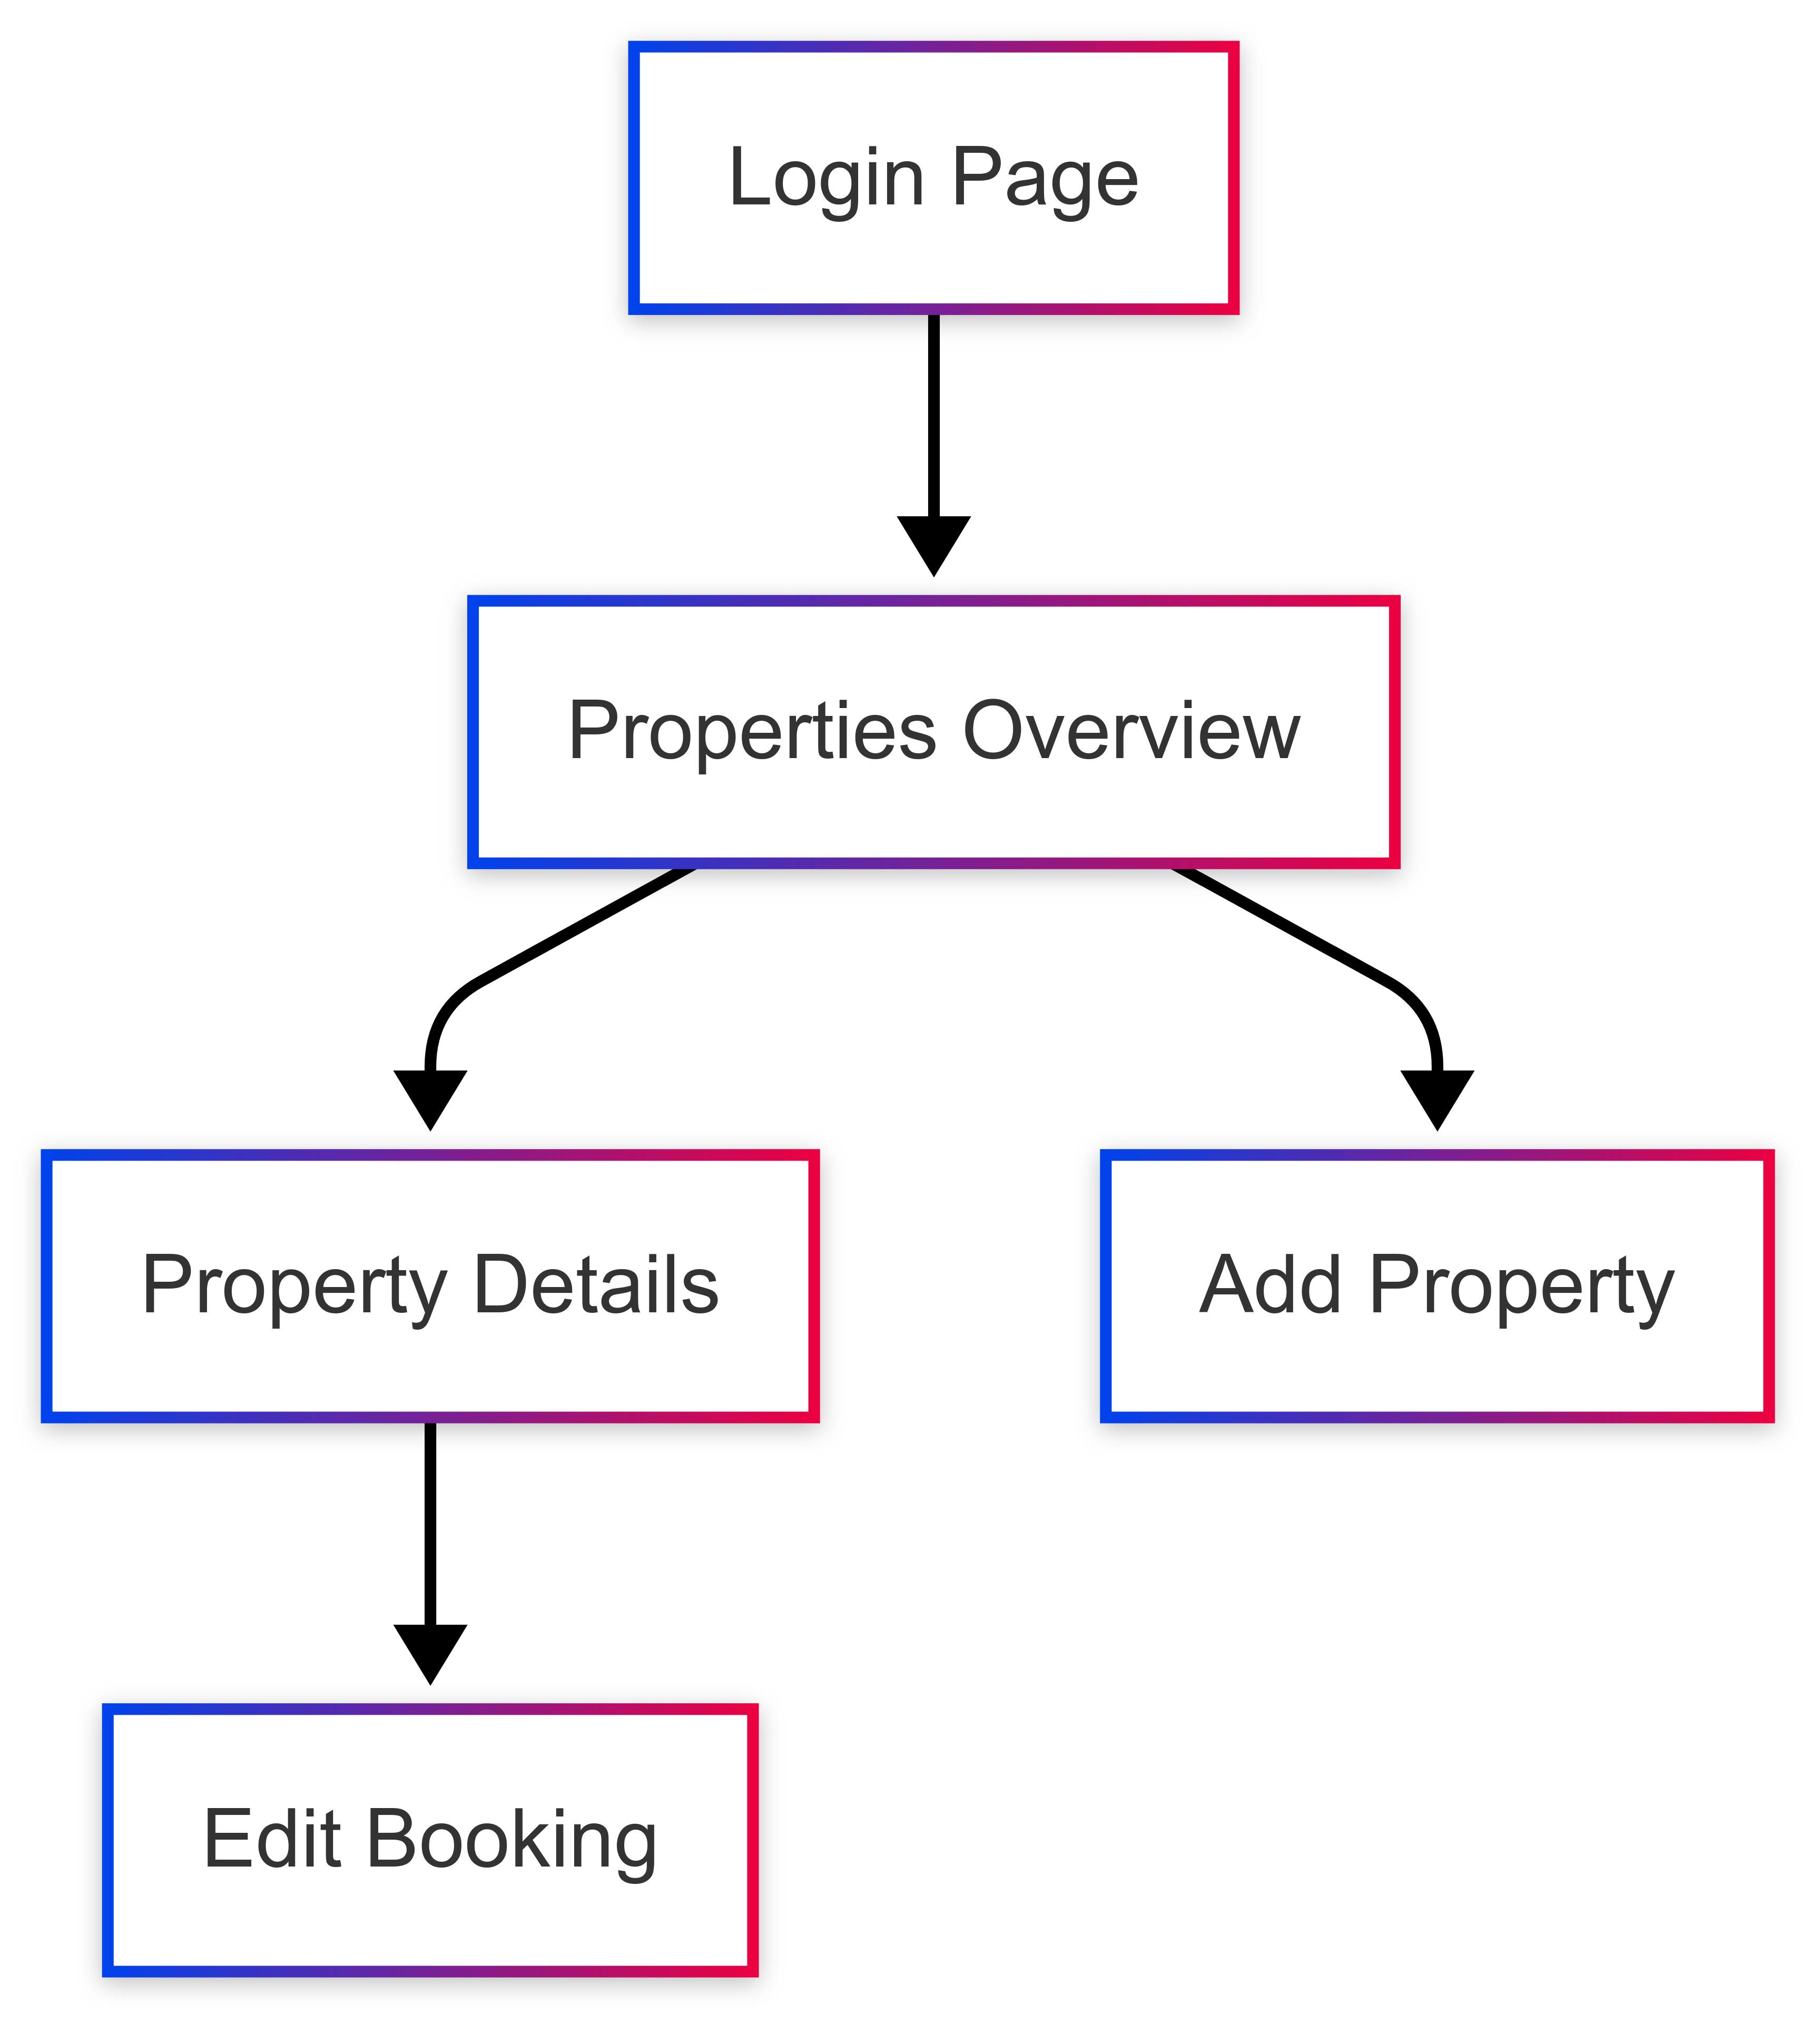
\includegraphics[width=0.55\textwidth]{images/StrukturDiagramm.png}
	\caption{Navigationsfluss der Mitarbeiteransicht}
	\label{fig:navigationsfluss}
\end{figure}

\begin{itemize}
	\item Der Einstiegspunkt ist die \textbf{Login-Seite}.
	\item Nach erfolgreichem Login gelangt man zur \textbf{Übersicht aller Immobilien} (Properties Overview).
	\item Von dort aus hat man zwei Hauptoptionen:
	\begin{itemize}
		\item \textbf{Links (Property Details)}: Details zu bestehenden Immobilien ansehen, mit der Möglichkeit, \textbf{Buchungen zu bearbeiten (Edit Booking)}.
		\item \textbf{Rechts (Add Property)}: Neue Immobilien hinzufügen.
	\end{itemize}
\end{itemize}


\subsection{Bibliotheken und Module}

\subsubsection{Importe}

Die Implementierung der Equilibria Sharing-Mitarbeiteransicht basiert auf einer Vielzahl von Bibliotheken und Modulen, die im Folgenden nach Kategorien zusammengefasst werden.
\begin{lstlisting}[language=JavaScript, caption={Kernimporte der Anwendung.}, label={listing:core-imports}]
import { redirect } from 'next/navigation'
import { useRouter } from 'next/navigation'
import { cookies } from 'next/headers'
import Image from 'next/image'
		
// Authentifizierung
import { compare } from 'bcrypt'
import { getSession } from '@/lib/session'
		
// Datenbankzugriff
import { prisma } from '@/lib/prisma'
		
// UI-Basiskomponenten
import { Button } from '@/components/ui/button'
import { Card } from '@/components/ui/card'
		
// Server-Actions
import { createProperty, updateProperty } from '@/app/actions/properties'
import { login } from '@/app/actions/auth'
\end{lstlisting}

Die in [\ref{listing:core-imports}] zusammengefassten Kernimporte repräsentieren die fundamentalen Technologien und Module, auf denen die Anwendung basiert. Next.js stellt mit \texttt{redirect}, \texttt{useRouter} und \texttt{cookies} essentielle Funktionen für Routing und Zustandsverwaltung bereit. Die Authentifizierung wird durch \texttt{bcrypt} für sichere Passwortvergleiche und die eigene \texttt{getSession}-Funktion realisiert. Der Datenbankzugriff erfolgt zentral über den \texttt{prisma}-Client, der eine sichere Interaktion mit der Datenbank ermöglicht. Für die Benutzeroberfläche werden grundlegende UI-Komponenten wie \texttt{Button} und \texttt{Card} verwendet. Die Server-Actions \texttt{login}, \texttt{createProperty} und \texttt{updateProperty} bilden das Rückgrat der serverseitigen Datenverarbeitung und gewährleisten eine sichere Handhabung sensibler Operationen.



\subsection{Authentifizierung und Sitzungsverwaltung}
\subsubsection{Login-Implementierung}
\begin{lstlisting}[language=JavaScript, caption={Benutzersuche in der Datenbank.}, label={listing:user-lookup}]
export async function login(email: string, password: string) {
	const user = await prisma.user.findUnique({
		where: { email }
	})
			
	if (!user) return { success: false, error: 'Benutzer nicht gefunden' }
\end{lstlisting}
	
	Die in [\ref{listing:user-lookup}] implementierte \texttt{login}-Funktion initiiert den Authentifizierungsprozess mit einer Datenbankabfrage. Mittels Prisma ORM wird ein Benutzer anhand seiner E-Mail-Adresse gesucht. Die frühzeitige Überprüfung auf Nichtexistenz des Benutzers stellt einen effizienten Kontrollfluss sicher und verhindert unnötige Folgeoperationen.
	
\begin{lstlisting}[language=JavaScript, caption={Passwortvalidierung und Sitzungserstellung.}, label={listing:password-validation}]
	const passwordValid = await compare(password, user.password)
			
		if (!passwordValid) return { success: false, error: 'Falsches Passwort' }
			
		const session = await createSession(user.id)
		cookies().set('session_id', session.id, { httpOnly: true })
\end{lstlisting}
	
	Der Codeabschnitt in [\ref{listing:password-validation}] realisiert zwei kritische Sicherheitsfunktionen. Zunächst erfolgt die Validierung des eingegebenen Passworts gegen den gespeicherten Hash mittels der \texttt{compare}-Funktion aus bcrypt. Bei erfolgreicher Authentifizierung wird anschließend eine neue Benutzersitzung erstellt und ein entsprechendes Cookie gesetzt. Die Verwendung des \texttt{httpOnly}-Flags verhindert dabei den Zugriff auf das Cookie via JavaScript, was einen wichtigen Schutz gegen XSS-Angriffe darstellt.
	
\begin{lstlisting}[language=JavaScript, caption={Rückgabeobjekt nach erfolgreicher Authentifizierung.}, label={listing:auth-return}]
return { 
	success: true, 
	user: { 
		id: user.id, 
		email: user.email, 
		name: user.name, 
		role: user.role 
	} 
}
\end{lstlisting}


Die Funktion schließt, wie in [\ref{listing:auth-return}] zu sehen, mit der Rückgabe eines strukturierten Objekts. Dieses signalisiert durch das \texttt{success}-Flag den erfolgreichen Abschluss des Authentifizierungsvorgangs und stellt gleichzeitig relevante Benutzerinformationen bereit. Bemerkenswert ist hierbei die bewusste Exklusion des Passwort-Hashes, was dem Prinzip der minimalen Datenweitergabe entspricht und die Sicherheit erhöht.

\subsubsection{Sitzungsverwaltung}

\begin{lstlisting}[language=JavaScript, caption={Erstellung einer neuen Sitzung.}, label={listing:session-create}]
return prisma.session.create({
	data: {
		userId,
		expiresAt: new Date(Date.now() + 30 * 24 * 60 * 60 * 1000) // 30 Tage
	}
})
\end{lstlisting}

Der in [\ref{listing:session-create}] dargestellte Funktion realisiert die Erzeugung eines neuen Sitzungseintrags in der Datenbank. Die Gültigkeitsdauer wird auf 30 Tage festgelegt, was einen angemessenen Kompromiss zwischen Benutzerkomfort und Sicherheit darstellt. Die Verknüpfung mit dem Benutzer erfolgt über die \texttt{userId}, wodurch eine eindeutige Zuordnung gewährleistet wird.

\begin{lstlisting}[language=JavaScript, caption={Abrufen einer bestehenden Sitzung.}, label={listing:session-get}]
export async function getSession() {
	const sessionId = cookies().get('session_id')?.value
		
	if (!sessionId) return null
		
	const session = await prisma.session.findUnique({
		where: { id: sessionId },
		include: { user: true }
	})
\end{lstlisting}

	
	Die Funktion \texttt{getSession()} in [\ref{listing:session-get}] bildet das Gegenstück zur Sitzungserstellung. Sie extrahiert zunächst die Sitzungs-ID aus dem Cookie-Speicher und führt eine frühzeitige Validierung durch. Diese Implementierung folgt dem Fail-Fast-Prinzip, indem sie bei fehlendem Cookie sofort abbricht und \texttt{null} zurückgibt, was die Effizienz des Codes erhöht.
	
\begin{lstlisting}[language=JavaScript, caption={Validierung der Sitzungsgültigkeit.}, label={listing:session-validate}]
if (!session || session.expiresAt < new Date()) {
	cookies().delete('session_id')
	return null
}
\end{lstlisting}


Der Codeausschnitt in [\ref{listing:session-validate}] führt eine zweistufige Validierung durch. Zunächst wird die Existenz der Sitzung in der Datenbank überprüft, gefolgt von einer Evaluation der zeitlichen Gültigkeit. Die automatische Bereinigung durch Löschen des Cookies bei ungültigen Sitzungen stellt einen proaktiven Sicherheitsmechanismus dar und verhindert potenzielle Inkonsistenzen zwischen Cookie-Zustand und Datenbankzustand.

\begin{lstlisting}[language=JavaScript, caption={Rückgabe der validierten Sitzung.}, label={listing:session-return}]
return session
\end{lstlisting}


Die in [\ref{listing:session-return}] gezeigte Rückgabe der vollständigen Sitzung inklusive der verknüpften Benutzerdaten (durch \texttt{include: \{ user: true \}}) ermöglicht einen effizienten Zugriff auf alle relevanten Informationen in einem einzigen Datenbankaufruf. Diese Optimierung reduziert die Anzahl der Datenbankabfragen und verbessert somit die Performanz der Anwendung.

\begin{lstlisting}[language=JavaScript, caption={Middleware für Routenschutz.}, label={listing:middleware-init}]
// middleware.ts
	
export function middleware(request: NextRequest) {
	const sessionId = request.cookies.get('session_id')?.value
\end{lstlisting}


Die in [\ref{listing:middleware-init}] implementierte Middleware stellt einen zentralen Baustein im Sicherheitskonzept der Anwendung dar. Sie nutzt die Next.js-Middleware-Funktionalität, um Anfragen vor dem Erreichen der eigentlichen Routen zu interceptieren. Die Extraktion der Sitzungs-ID aus den Cookies erfolgt hier direkt auf Request-Ebene, was eine effiziente Verarbeitung ermöglicht.

\begin{lstlisting}[language=JavaScript, caption={Umleitung nicht authentifizierter Anfragen.}, label={listing:middleware-redirect}]
if (!sessionId && !request.nextUrl.pathname.startsWith('/login')) {
	return NextResponse.redirect(new URL('/login', request.url))
}
		
return NextResponse.next()
}
\end{lstlisting}


Der in [\ref{listing:middleware-redirect}] dargestellte Codeblock realisiert eine automatische Umleitung nicht authentifizierter Benutzer zur Login-Seite. Die Implementierung berücksichtigt dabei intelligent den aktuellen Pfad, um Weiterleitungsschleifen zu vermeiden. Durch die Verwendung von Next.js Response-Objekten erfolgt die Umleitung serverseitig, was zusätzliche Sicherheit bietet und clientseitige Manipulationen verhindert.





\subsection{Benutzeroberfläche und Interaktionsdesign}
\subsubsection{Immobilie Übersicht}

\begin{figure}
\centering
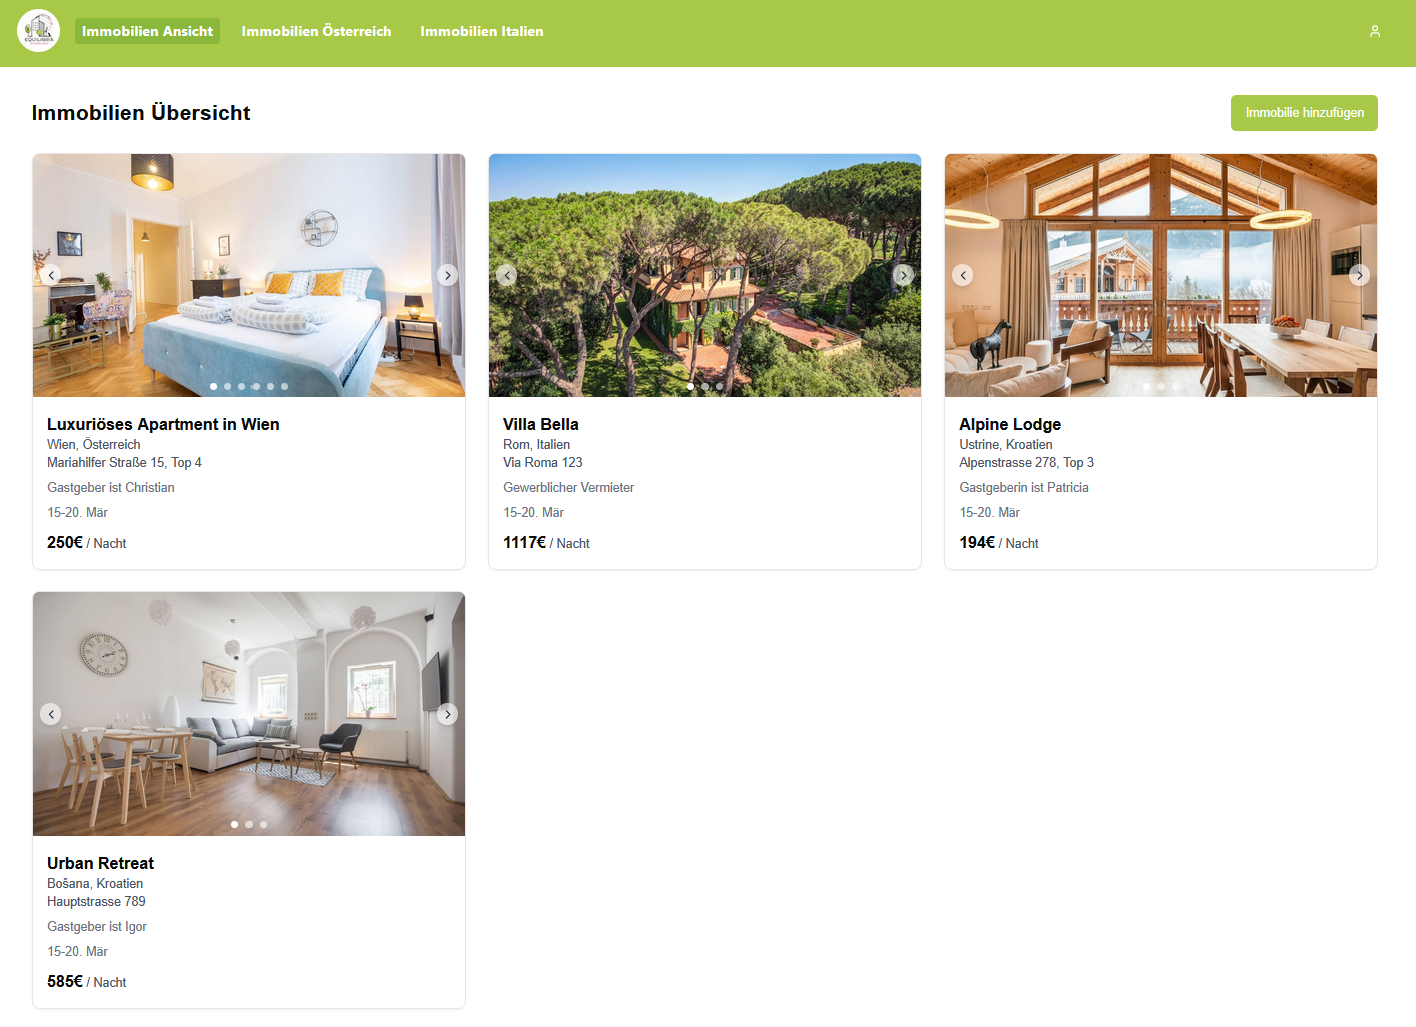
\includegraphics[width=0.80\textwidth]{images/Immobilien_Uebersicht.png}
\caption{Übersicht über alle Immobilien}
\end{figure}


\begin{lstlisting}[language=JavaScript, caption={Datenabruf für die Immobilien-Übersicht.}, label={listing:property-data-fetch}]
export default async function DashboardPage() {
	const session = await getSession()
		
	if (!session) {
		redirect('/login')
	}
		
	const properties = await prisma.property.findMany({
		where: { organizationId: session.user.organizationId },
	})
\end{lstlisting}

	
	Die Hauptkomponente in [\ref{listing:property-data-fetch}] implementiert einen serverseitigen Datenabruf. Zunächst erfolgt eine Authentifizierungsprüfung mit automatischer Weiterleitung zur Login-Seite bei fehlender Sitzung. Anschließend werden alle Immobilien der Organisation des angemeldeten Benutzers aus der Datenbank abgerufen, was eine effektive Zugriffskontrolle auf Organisationsebene realisiert.

\newpage
    
\begin{lstlisting}[language=JavaScript, caption={Header-Bereich der Übersichtsseite.}, label={listing:property-header}]
return (
<div className="container mx-auto px-4 py-8">
<div className="mb-6 flex items-center justify-between">
<h1 className="text-2xl font-bold">Immobilien Übersicht</h1>
<a href="/properties/new" className="rounded bg-primary px-4 py-2 text-white">
	Neue Immobilie
</a>
</div>
)
\end{lstlisting}

	
	Der in [\ref{listing:property-header}] implementierte Header-Bereich kombiniert einen aussagekräftigen Titel zum Hinzufügen neuer Immobilien. Die Verwendung von Tailwind CSS-Klassen ermöglicht ein responsives Layout mit konsistenten Abständen. Die semantische Struktur mit \texttt{h1} für die Hauptüberschrift verbessert zudem die Zugänglichkeit und SEO-Eigenschaften der Seite.
	
\begin{lstlisting}[language=JavaScript, caption={Rasterdarstellung der Immobilien.}, label={listing:property-grid}]
<div className="grid gap-6 md:grid-cols-2 lg:grid-cols-3">
	{properties.map((property) => (
		<PropertyCard 
		      key={property.id}
		      property={property}
		      href={`/properties/{property.id}`}
	       />
	))}
\end{lstlisting}

	
	Der in [\ref{listing:property-grid}] dargestellte Code realisiert ein responsives Raster zur Anzeige der Immobilien. Durch die Verwendung von CSS Grid mit unterschiedlichen Spaltenanzahlen je nach Bildschirmgröße wird eine optimale Darstellung auf verschiedenen Geräten gewährleistet. Die Iteration über das \texttt{properties}-Array mit der \texttt{map}-Funktion erzeugt für jede Immobilie eine \texttt{PropertyCard}-Komponente mit eindeutigem Schlüssel und Detaillink.
	
	
\begin{lstlisting}[language=JavaScript, caption={Definition der Immobilienkarten-Komponente.}, label={listing:property-card-def}]
// components/property-card.tsx

export default function PropertyCard({ property, href }) {
\end{lstlisting}

		
		Die in [\ref{listing:property-card-def}] definierte \texttt{PropertyCard}-Komponente dient der einheitlichen Darstellung von Immobilieninformationen. Die Verwendung von spezifischen Komponenten wie \texttt{Image} und \texttt{Link} optimiert die Ladezeiten und Navigation. Die importierten Icons aus der Lucide-Bibliothek ermöglichen eine intuitive visuelle Darstellung von Immobilienmerkmalen wie Standort, Schlafzimmern und Badezimmern.
		
\begin{lstlisting}[language=JavaScript, caption={Datenextraktion und Container-Struktur.}, label={listing:property-card-structure}]
const { title, price, address, bedrooms, bathrooms, area, images } = property
const imageUrl = images[0]?.url || '/placeholder.jpg'

return (
	<Link href={href} className="group overflow-hidden rounded-lg border shadow transition hover:shadow-md">
	<div className="relative h-48 w-full">
)
\end{lstlisting}

		
		Der Codeabschnitt in [\ref{listing:property-card-structure}] zeigt die Destrukturierung der Immobiliendaten und den Beginn der Kartenstruktur. Die Verwendung eines Fallback-Bildes gewährleistet eine konsistente Darstellung auch bei fehlenden Bilddaten. Der umschließende \texttt{Link} macht die gesamte Karte klickbar, während die CSS-Klassen für visuelle Effekte wie Schatten und abgerundete Ecken sorgen.
		
\begin{lstlisting}[language=JavaScript, caption={Optimierte Bilddarstellung.}, label={listing:property-image}]
<Image
	src={imageUrl || "/placeholder.svg"}
	alt={title}
	fill
	className="object-cover transition-transform group-hover:scale-105"
	sizes="(max-width: 768px) 100vw, (max-width: 1200px) 50vw, 33vw"
/>
\end{lstlisting}

		
		Die in [\ref{listing:property-image}] implementierte Bilddarstellung nutzt die \texttt{Image}-Komponente von Next.js für optimierte Ladezeiten und automatische Bildgrößenanpassung. Das \texttt{fill}-Attribut sorgt dafür, dass das Bild den Container vollständig ausfüllt, während \texttt{object-cover} ein gleichmäßiges Seitenverhältnis gewährleistet. Der Hover-Effekt mit leichter Vergrößerung (\texttt{scale-105}) bietet subtiles visuelles Feedback bei Benutzerinteraktion.
		
		
\begin{lstlisting}[language=JavaScript, caption={Darstellung der Immobilienmerkmale.}, label={listing:property-features}]
<div className="grid grid-cols-3 gap-2 text-sm">
<div className="flex items-center">
<BedDouble className="mr-1 h-4 w-4" />
<span>{bedrooms} {bedrooms === 1 ? 'Zimmer' : 'Zimmer'}</span>
</div>
<div className="flex items-center">
<Bath className="mr-1 h-4 w-4" />
\end{lstlisting}

		
		Die in [\ref{listing:property-features}] implementierte Darstellung der Immobilienmerkmale nutzt ein dreispaltiges Grid-Layout für eine übersichtliche Anordnung. Jedes Merkmal wird durch ein passendes Icon visualisiert und mit dem entsprechenden Wert kombiniert. Die bedingte Textausgabe berücksichtigt die Singular- und Pluralformen, was die sprachliche Korrektheit der Benutzeroberfläche verbessert.
		
		
		
		
		\subsubsection{Immobilie Hinzufügen}
		
		\begin{figure}
			\centering
			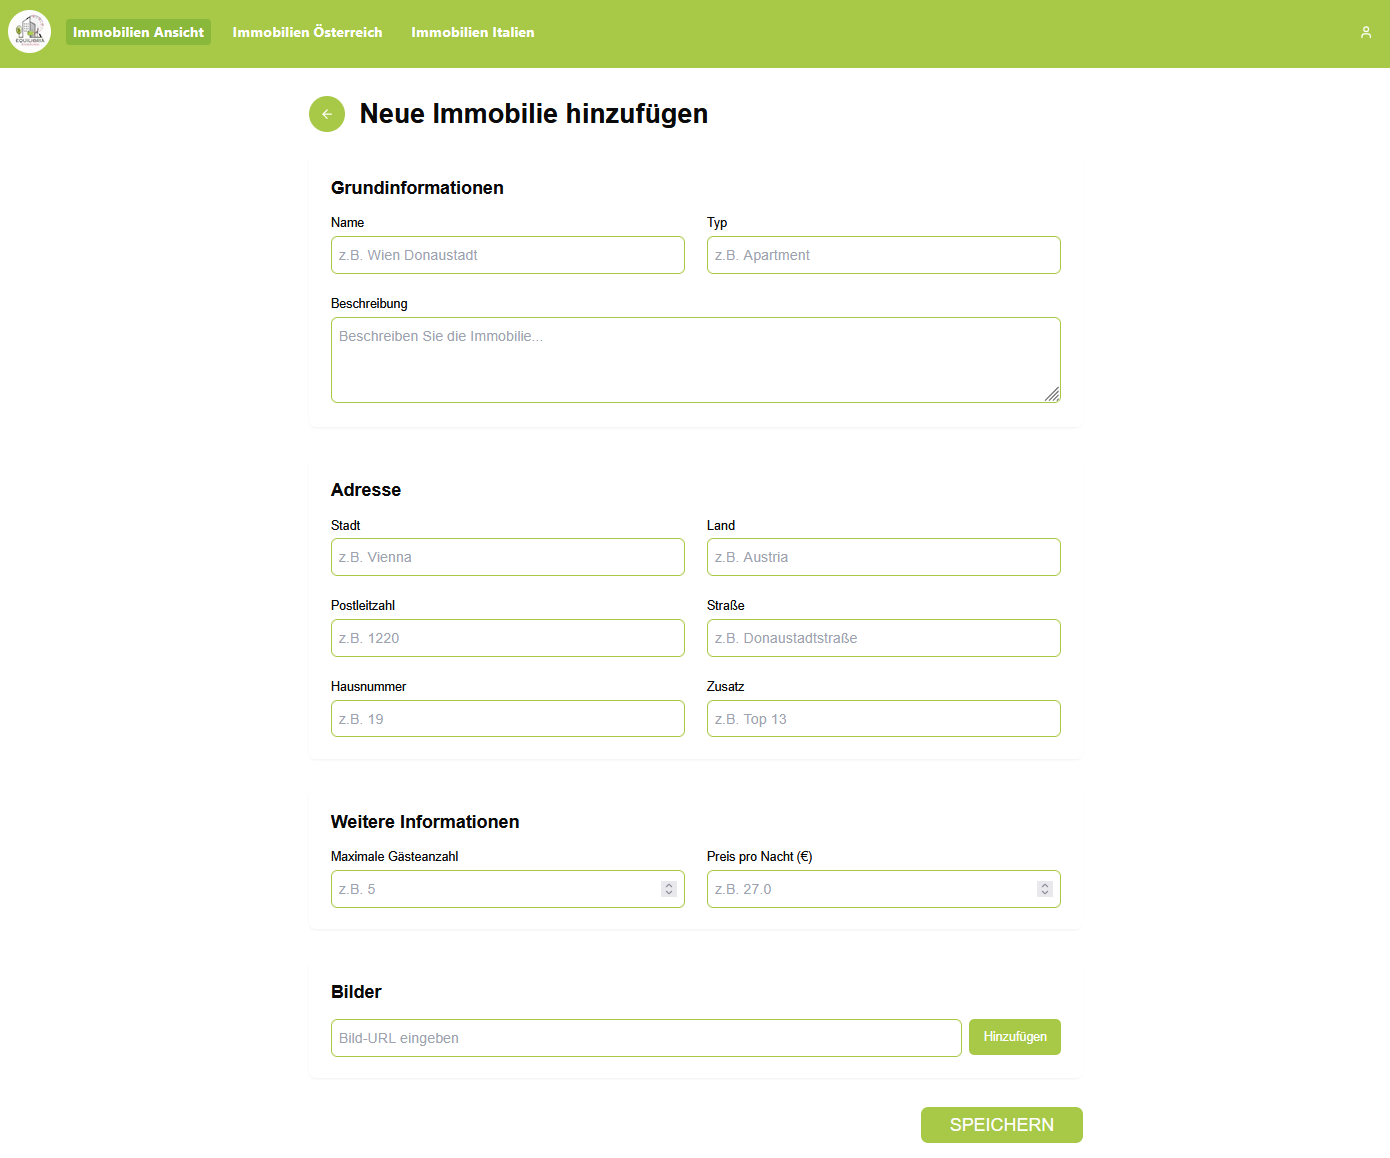
\includegraphics[width=0.80\textwidth]{images/Immobilien_hinzufuegen.png}
			\caption{Seite zum Hinzufügen von Immobilien}
		\end{figure}
		
		
\begin{lstlisting}[language=JavaScript, caption={Authentifizierungsprüfung und Container-Struktur.}, label={listing:property-add-auth}]
export default async function NewPropertyPage() {
	const session = await getSession()
					
	if (!session) {
		redirect('/login')
	}
					
	return (
	    <div className="container mx-auto px-4 py-8">
)
\end{lstlisting}

			
			Die Hauptkomponente in [\ref{listing:property-add-auth}] beginnt mit einer Authentifizierungsprüfung, die nicht angemeldete Benutzer zur Login-Seite weiterleitet. Diese Sicherheitsmaßnahme stellt sicher, dass nur autorisierte Benutzer neue Immobilien hinzufügen können. Der Container mit definierten Abständen sorgt für eine konsistente Darstellung und optimale Lesbarkeit auf verschiedenen Bildschirmgrößen.

\newpage

\begin{lstlisting}[language=JavaScript, caption={Beginn des Formularinhalts.}, label={listing:property-form-content-start}]
<form onSubmit={handleSubmit} className="space-y-6">
<div className="grid gap-6 md:grid-cols-2">
<div>
<label htmlFor="title" className="block text-sm font-medium">
Titel
</label>
\end{lstlisting}

			
			Der in [\ref{listing:property-form-content-start}] dargestellte Beginn des Formularinhalts zeigt die Verwendung eines responsiven Grid-Layouts für eine optimale Raumnutzung. Die zweispaltige Anordnung auf größeren Bildschirmen verbessert die Übersichtlichkeit und reduziert die vertikale Ausdehnung des Formulars. Die semantische Verknüpfung von Labels und Eingabefeldern durch die \texttt{htmlFor}-Attribute verbessert die Zugänglichkeit.
			
			
\begin{lstlisting}[language=JavaScript, caption={Einbindung des Immobilienformulars.}, label={listing:property-add-form}]
<PropertyForm 
	organizationId={session.user.organizationId}
	userId={session.user.id}
/>
\end{lstlisting}

		
		Die in [\ref{listing:property-add-form}] dargestellte Einbindung des Immobilienformulars übergibt wichtige Kontextinformationen aus der Benutzersitzung. Die Organisations-ID ermöglicht die korrekte Zuordnung der neuen Immobilie zur Organisation des Benutzers, während die Benutzer-ID für Audit-Zwecke und die Nachverfolgung von Änderungen verwendet wird. Diese Implementierung folgt dem Prinzip der Datensparsamkeit, indem nur die notwendigen Informationen weitergegeben werden.
		
		
\begin{lstlisting}[language=JavaScript, caption={Initialisierung der Formularkomponente.}, label={listing:property-form-init}]
export default function PropertyForm({ organizationId, userId, initialData }) {
	const router = useRouter()
	const [loading, setLoading] = useState(false)
	const [error, setError] = useState('')
					
	const [formData, setFormData] = useState(initialData || {
		title: '',
		description: '',
		price: '',
\end{lstlisting}

				
				Die Formularkomponente in [\ref{listing:property-form-init}] implementiert eine flexible Initialisierung, die sowohl für neue Immobilien als auch für die Bearbeitung bestehender Immobilien geeignet ist. Die Verwendung von \texttt{initialData} als optionaler Parameter ermöglicht die Vorausfüllung des Formulars mit existierenden Daten. Die Zustandsvariablen für Ladezustand und Fehler verbessern das Feedback während der Formularverarbeitung.
				
                
\begin{lstlisting}[language=JavaScript, caption={Behandlung von Formularänderungen.}, label={listing:property-form-change}]
const handleChange = (e) => {
	const { name, value } = e.target
				
	if (name.includes('.')) {
		const [parent, child] = name.split('.')
		setFormData({
			...formData,
			[parent]: { ...formData[parent], [child]: value }
		})
	}
}
\end{lstlisting}

						
						Die in [\ref{listing:property-form-change}] implementierte \texttt{handleChange}-Funktion ermöglicht die Aktualisierung verschachtelter Formularfelder. Durch die Analyse des Feldnamens wird erkannt, ob es sich um ein einfaches oder ein verschachteltes Feld handelt. Bei verschachtelten Feldern wie Adresskomponenten wird die entsprechende Unterstruktur im Formularstatus aktualisiert, ohne andere Werte zu beeinflussen.
						
						
\begin{lstlisting}[language=JavaScript, caption={Datenvorbereitung für die Übermittlung.}, label={listing:property-form-prepare}]
try {
	// Daten für die Übermittlung vorbereiten
	const propertyData = {
		...formData,
		price: parseFloat(formData.price),
		bedrooms: parseInt(formData.bedrooms, 10),
		bathrooms: parseInt(formData.bathrooms, 10),
		area: parseFloat(formData.area),
\end{lstlisting}

								
								Die in [\ref{listing:property-form-prepare}] dargestellte Datenvorbereitung konvertiert Zeichenkettenwerte aus dem Formular in die entsprechenden numerischen Typen. Diese Typkonvertierung ist entscheidend für die korrekte Verarbeitung in der Datenbank und verhindert potenzielle Fehler bei mathematischen Operationen oder Sortierungen. Die Verwendung von \texttt{parseFloat} und \texttt{parseInt} mit expliziter Angabe der Basis gewährleistet konsistente Ergebnisse.
\begin{lstlisting}[language=JavaScript, caption={Aufruf der Server-Action.}, label={listing:property-form-action}]
        organizationId,
        userId
    }

	// Server-Action aufrufen
	const result = await createProperty(propertyData)

	if (result.success) {
		router.push(`/properties/${result.id}`)
\end{lstlisting}

								
								Der in [\ref{listing:property-form-action}] implementierte Aufruf der Server-Action übergibt die vorbereiteten Daten an die serverseitige Funktion \texttt{createProperty}. Bei erfolgreicher Erstellung wird der Benutzer automatisch zur Detailseite der neuen Immobilie weitergeleitet.
								
\begin{lstlisting}[language=JavaScript, caption={Fehlerbehandlung bei der Formularübermittlung.}, label={listing:property-form-error}]
	router.refresh()
} else {
	setError(result.error || 'Ein Fehler ist aufgetreten')
}
} catch (err) {
	setError('Serverfehler. Bitte später erneut versuchen.')
	console.error(err)
} finally {
	setLoading(false)
}
\end{lstlisting}

					
					Die in [\ref{listing:property-form-error}] gezeigte Fehlerbehandlung fängt sowohl explizite Fehlermeldungen von der Server-Action als auch unerwartete Ausnahmen ab. Die Verwendung eines Try-Catch-Finally-Blocks gewährleistet, dass der Ladezustand in jedem Fall zurückgesetzt wird, unabhängig vom Ergebnis der Operation. Die Protokollierung von Fehlern in der Konsole erleichtert die Fehlersuche während der Entwicklung.
					
					
					
					\subsubsection{Immobilien Details}
					
					\begin{figure}
						\centering
						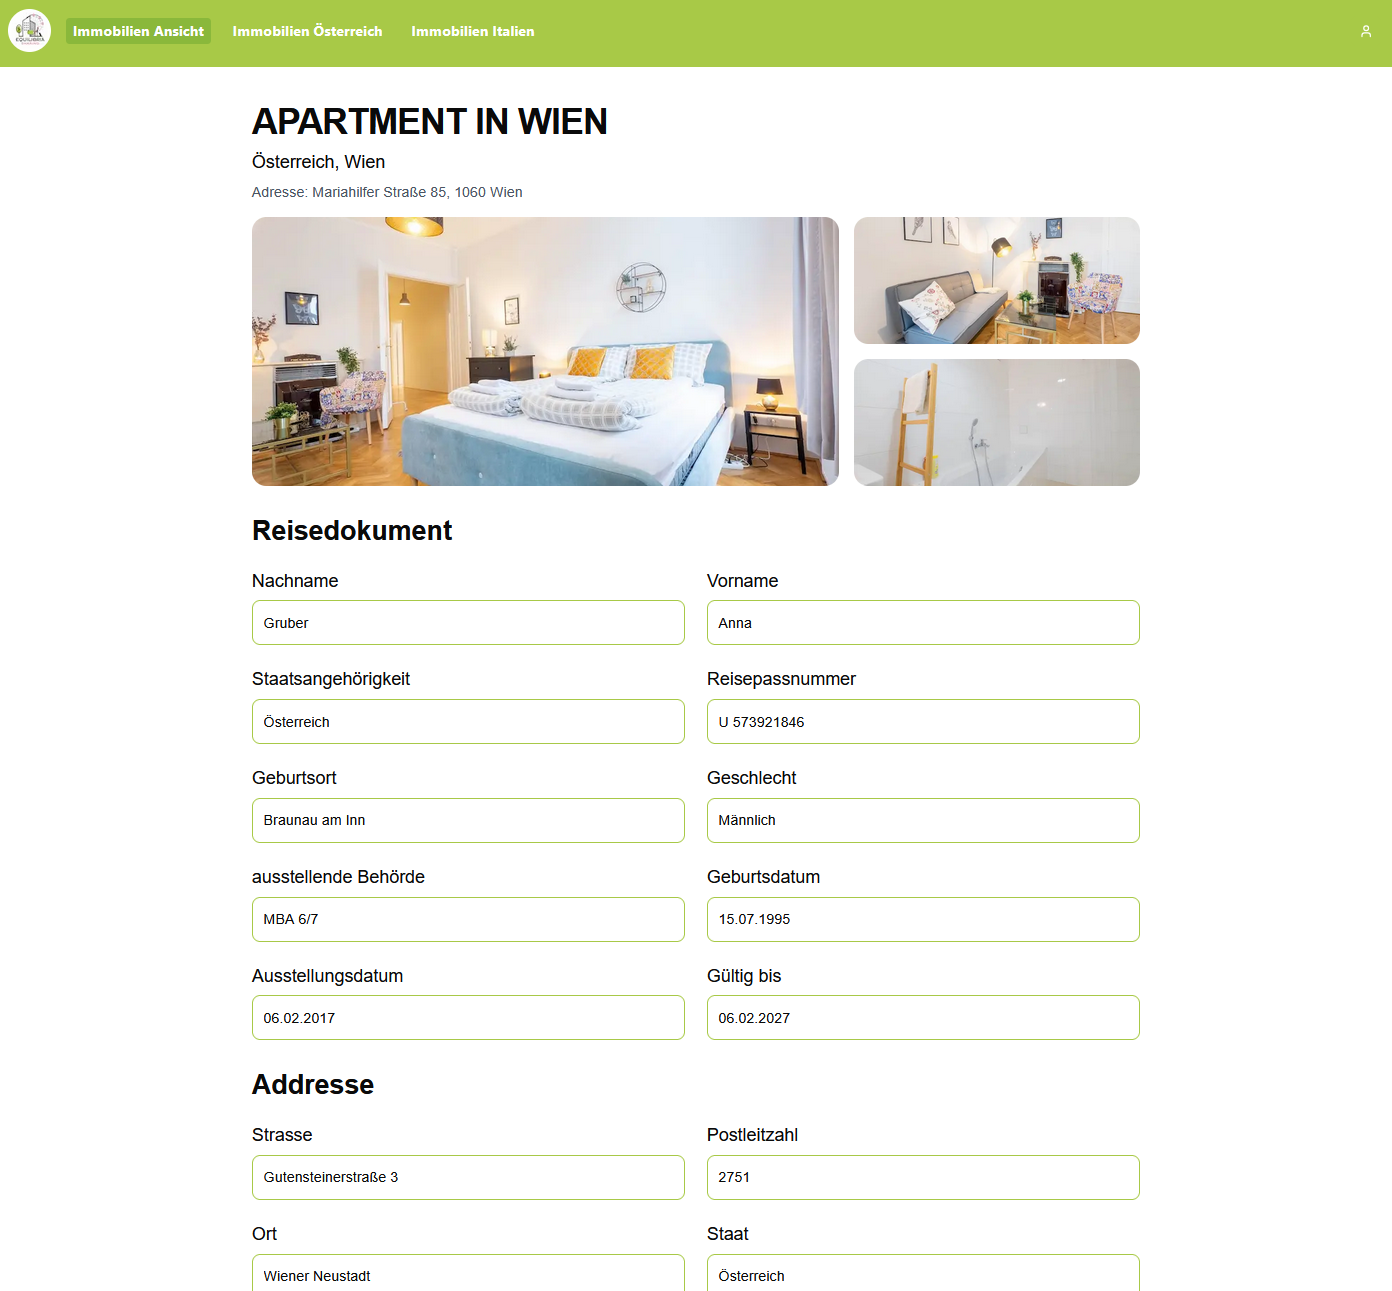
\includegraphics[width=0.80\textwidth]{images/Immobilien_bearbeiten.png}
						\caption{Buchung Bearbeitungsseite}
					\end{figure}
\begin{lstlisting}[language=JavaScript, caption={Authentifizierung und Datenabruf.}, label={listing:property-details-auth}]
export default async function PropertyPage({ params }) {
	const session = await getSession()

	if (!session) {
		redirect('/login')
	}

	const property = await prisma.property.findUnique({
		where: { id: params.id },
\end{lstlisting}

							
							Die Hauptkomponente in [\ref{listing:property-details-auth}] beginnt mit einer Authentifizierungsprüfung und leitet nicht angemeldete Benutzer zur Login-Seite weiter. Anschließend wird die spezifische Immobilie anhand der in den URL-Parametern übergebenen ID aus der Datenbank abgerufen. Diese serverseitige Datenabfrage gewährleistet, dass die Seite bereits beim ersten Laden vollständige Informationen enthält.
							
\newpage
                            
\begin{lstlisting}[language=JavaScript, caption={Zugriffskontrolle.}, label={listing:property-details-access}]
if (!property) {
	notFound()
}

// Prüfen, ob der Benutzer Zugriff auf diese Immobilie hat
if (property.organizationId !== session.user.organizationId) {
	redirect('/dashboard')
}
\end{lstlisting}

							
							Der in [\ref{listing:property-details-access}] implementierte Zugriffskontrollmechanismus stellt sicher, dass Benutzer nur auf Immobilien ihrer eigenen Organisation zugreifen können. Falls die Immobilie nicht existiert, wird die Next.js \texttt{notFound}-Funktion aufgerufen, die eine standardisierte 404-Seite rendert. Bei unberechtigtem Zugriff erfolgt eine Weiterleitung zum Dashboard, was potenzielle Sicherheitslücken durch URL-Manipulation verhindert.
							
\begin{lstlisting}[language=JavaScript, caption={Einbindung der Detailkomponente.}, label={listing:property-details-component}]
<PropertyDetails property={property} />
</div>
)
}
\end{lstlisting}

						
						Die in [\ref{listing:property-details-component}] gezeigte Einbindung der \texttt{PropertyDetails}-Komponente kapselt die eigentliche Darstellung der Immobilieninformationen. Diese Trennung von Datenabfrage und Präsentation folgt dem Prinzip der Separation of Concerns und verbessert die Wartbarkeit des Codes. Die Übergabe des vollständigen Immobilienobjekts als Prop ermöglicht eine flexible Darstellung aller verfügbaren Informationen.
						
\begin{lstlisting}[language=JavaScript, caption={Struktur der Detailkomponente.}, label={listing:property-details-structure}]
export default function PropertyDetails({ property }) {
	const { title, description, price, bedrooms, bathrooms, area, images, address, 
		createdAt, updatedAt, createdBy } = property

	return (
		<div className="grid gap-8 md:grid-cols-3">
		<div className="md:col-span-2">
\end{lstlisting}

							
							Die in [\ref{listing:property-details-structure}] implementierte Struktur der Detailkomponente verwendet ein responsives Grid-Layout, das auf größeren Bildschirmen eine asymmetrische Aufteilung mit zwei Dritteln für Hauptinhalte und einem Drittel für Zusatzinformationen bietet. Die Destrukturierung des Immobilienobjekts am Anfang der Komponente verbessert die Lesbarkeit des Codes und vereinfacht den Zugriff auf die einzelnen Eigenschaften.
\newpage
                            
\begin{lstlisting}[language=JavaScript, caption={Bilddarstellung.}, label={listing:property-details-image}]
<div className="mb-6 overflow-hidden rounded-lg">
{images && images.length > 0 ? (
    <div className="relative h-[400px] w-full">
	<Image
		src={images[0].url || "/placeholder.svg"}
	    alt={title}
	    fill
		className="object-cover"
	/>
</div>
\end{lstlisting}

								
								Die in [\ref{listing:property-details-image}] gezeigte Bilddarstellung implementiert eine bedingte Logik, die prüft, ob Bilder vorhanden sind. Das Hauptbild wird in einem Container mit fester Höhe und voller Breite dargestellt, wobei die \texttt{object-cover}-Eigenschaft ein gleichmäßiges Seitenverhältnis gewährleistet. Die Verwendung der Next.js \texttt{Image}-Komponente optimiert die Ladezeit und Bildqualität.
								
								
\begin{lstlisting}[language=JavaScript, caption={Galerie für zusätzliche Bilder.}, label={listing:property-details-gallery}]
{images && images.length > 1 && (
<div className="mb-6 grid grid-cols-4 gap-2">
{images.slice(1, 5).map((image, index) => (
<div key={image.id} className="relative h-24 overflow-hidden rounded">
<Image
	src={image.url || "/placeholder.svg"}
	alt={`${title} - Bild ${index + 2}`}
\end{lstlisting}

										
										Die in [\ref{listing:property-details-gallery}] dargestellte Bildergalerie wird nur angezeigt, wenn mehr als ein Bild vorhanden ist. Die Anordnung in einem vierspaltigen Grid ermöglicht eine kompakte Darstellung von bis zu vier zusätzlichen Bildern. Die Verwendung von \texttt{slice(1, 5)} begrenzt die Anzahl der angezeigten Vorschaubilder und verhindert eine Überladung der Benutzeroberfläche.
										
										\subsection{Zusammenfassung der Implementierung}
										
										\subsubsection{Reflexion der Herausforderungen}
										Während der Implementierung traten verschiedene Herausforderungen auf, insbesondere in den Bereichen Authentifizierung, Zustandsmanagement und API-Integration. Die korrekte Implementierung der Authentifizierung mit NextAuth.js und der Integration mit dem Backend stellte sich als komplexer heraus, als ursprünglich gedacht, da verschiedene Benutzerrollen unterschiedliche Zugriffsrechte benötigten.
										
										Ein weiteres Problem war das Fehlerhandling bei API-Anfragen. Um sicherzustellen, dass Netzwerkfehler oder Backend-Probleme nicht zu einer schlechten Benutzererfahrung führen, wurde ein zentrales Error-Handling-System entwickelt, das Fehler abfängt, protokolliert und benutzerfreundliche Fehlermeldungen anzeigt.
										
										Schließlich war die größte Herausforderung die Verwaltung des Zustandsmanagements zwischen Server- und Client-Komponenten. Denn besonders hier ist es aufgrund der unterschiedlichen Ausführungsumgebungen oft zu unerwarteten Verhaltensweisen gekommen. Die Fehlermeldungen dieser Art von Problemen waren sehr schwer zu interpretieren, da sie oft erst zur Laufzeit auftraten. Schließlich wurde eine klare Trennung zwischen Server- und Client-Komponenten geschaffen, wobei Server-Komponenten für den Datenabruf und Client-Komponenten für die interaktiven Elemente zuständig sind, was zu einer robusteren Anwendung führte.
										
										Zusätzlich zu diesen technischen Herausforderungen verzögerte sich die Frontend-Entwicklung länger als ursprünglich geplant, hauptsächlich aufgrund der Komplexität der Benutzeroberfläche und der notwendigen Anpassungen für verschiedene Endgeräte. Erschwerend kam hinzu, dass im Backend ein subtiler Fehler in der API-Schnittstelle entdeckt wurde, der die vollständige Integration zwischen Frontend und Backend verhinderte. Dieser Fehler betraf insbesondere die Datenformate bei der Übertragung von Immobilieninformationen, wodurch die Verbindung zum Backend zum Zeitpunkt der Fertigstellung noch nicht vollständig implementiert werden konnte. Stattdessen wurde für Demonstrationszwecke eine Mock-API entwickelt, die das erwartete Verhalten des Backends simuliert.
										
										
										\subsubsection{Zukünftige Erweiterungen}
										Für zukünftige Versionen sind folgende Erweiterungen denkbar:
										\begin{itemize}
											\item \textbf{Erweiterte Filterfunktionen:} Implementierung von fortschrittlicheren Suchfiltern und Sortieroptionen für Immobilien, um Mitarbeiter eine präzisere Auswahl nach spezifischen Kriterien wie zum Beispiel Ausstattungsmerkmalen zu ermöglichen.
											
											\item \textbf{Interaktive Visualisierungen:} Integration von 3D-Modellen und virtuellen Rundgängen für Immobilien, um potenziellen Interessenten einen besseren Eindruck der Objekte zu vermitteln, ohne physisch vor Ort sein zu müssen.
											
											\item \textbf{Automatisierte End-to-End-Tests:} Ausbau der Testabdeckung durch Cypress oder Playwright Tests, um kritische Benutzerflüsse wie Anmeldung, Immobiliensuche und Kontaktanfragen automatisiert zu testen und die Anwendungsstabilität zu gewährleisten.
										\end{itemize}

\setauthor{ }
%!TEX root=../main.tex
\chapter{Retrospektive}

\section{Erreichte Ergebnisse}

Der zu Beginn des Projekts definierte Umfang konnte erfolgreich umgesetzt werden. Die geplante Webanwendung wurde funktionsfähig realisiert und bietet die Möglichkeit, Mieterdaten effizient zu erfassen, zu validieren, langfristig zu speichern und in strukturierter Form darzustellen. Darüber hinaus ermöglicht das System die Erstellung von Buchungsprotokollen sowie eine übersichtliche Darstellung aller bisherigen und zukünftigen Buchungen. Die definierten Anforderungen konnten zum Großteil im vorgesehenen Zeitrahmen erfüllt werden.

\section{Relevanz und Auswirkungen}

\subsection{Gesellschaftliche Relevanz}

Die Digitalisierung administrativer Prozesse gewinnt zunehmend an Bedeutung – insbesondere in kleinen und mittelständischen Unternehmen, die bislang oft mit manuellen oder inoffiziellen Kommunikationskanälen arbeiten. Durch unser Projekt wurde ein exemplarischer Beitrag zur digitalen Transformation in der Kurzzeitvermietung geleistet. Die Anwendung dient als Beispiel dafür, wie mit begrenzten Ressourcen ein praxisrelevantes IT-System umgesetzt werden kann, das echten Mehrwert für den operativen Alltag bietet.

\subsection{Wirtschaftliche und betriebliche Relevanz}

Für den Auftraggeber stellt die entwickelte Lösung einen wesentlichen Fortschritt dar. Die Arbeitsabläufe im Bereich der Mieterkommunikation, Datenerfassung und Buchungsübersicht konnten deutlich vereinfacht und beschleunigt werden. Durch die automatisierte Datenverarbeitung und die strukturierte Darstellung aller Buchungen wird nicht nur Zeit gespart, sondern auch die Fehleranfälligkeit reduziert. Darüber hinaus legt das Projekt die Grundlage für zukünftige Erweiterungen – etwa für mehrere Standorte oder zusätzliche Funktionalitäten.

\newpage

\section{Herausforderungen während der Umsetzung}

Während der Umsetzung des Projekts sind mehrere unerwartete Herausforderungen aufgetreten:

\begin{itemize}
    \item \textbf{Kommunikation im Team:} Trotz regelmäßiger Meetings und Kommunikation wurden Änderungen und Anforderungen an Schnittstellen, Datenstrukturen, etc. teilweise unzureichend kommuniziert, was besonders in der Implementierungsphase zu Missverständnissen führte. Die Frontend- und Backend Bereiche waren bis zur Mitte der Implementierungsphase komplett isoliert voneinander, was zu einem Mehraufwand geführt hat. Für zukünftige Projekte empfiehlt sich ein klar strukturierter Kommunikationsplan und regelmäßige, klar strukturierte Meetings.
    
    \item \textbf{Unterschätzung neuer Technologien:} Die Komplexität einiger Technologien - insbesondere im Frontend-Bereich - waren zu Projektbeginn für das Team noch weitgehend unbekannt. Dies führte stellenweise zu Verzögerungen, da notwendige Kenntnisse erst erarbeitet werden mussten. Hier hätten externe Experten oder gezieltere Vorab-Recherche geholfen.
\end{itemize}

\section{Verbesserungspotenzial}

Neben den bereits genannten Herausforderungen gibt es auch einige Verbesserungsvorschläge für zukünftige Iterationen des Projekts:

\begin{itemize}
    \item \textbf{Strukturiertere API-Dokumentation:} Die aktuell dokumentierten Schnittstellen sind funktional, jedoch fehlt es stellenweise an übersichtlichen Beispielen und klaren Response-Strukturen. Eine ausführlichere API-Dokumentation würde insbesondere externen Entwickler:innen den Einstieg erleichtern.
    
    \item \textbf{Beitragsrichtlinien und Git-Nutzung:} Während der Entwicklung arbeitete jedes Teammitglied an eigenen Branches. Für eine verbesserte Struktur wären interne Richtlinien sowie die Aufstellung spezifischer Userstories hilfreich gewesen.
    
    \item \textbf{Hosting und Deployment:} Das Projekt wurde bis jetzt noch nicht online bereitgestellt, was zu einer Verzögerung beim Testing führte. Dies hat die Folgen, dass das Projekt im dafür vorgesehenen Zeitraum nicht extern vom Projektteam oder vom Auftraggeber getestet werden konnte.
\end{itemize} \cite{prompt-gpt-write-retrospektive}


%!TEX root=../main.tex
\chapter{Conclusio} 

Im Rahmen dieser Diplomarbeit wurde ein webbasiertes System zur Erfassung, Verwaltung und Darstellung von Mieterdaten für die Equilibria GmbH konzipiert und prototypisch umgesetzt. Ziel war es, bestehende manuelle Prozesse – insbesondere die dezentrale Kommunikation über Messenger-Dienste – durch eine zentrale, benutzerfreundliche und skalierbare Softwarelösung zu ersetzen.

Die im Projekt entwickelten Komponenten erfüllen die zuvor definierten funktionalen Anforderungen: Ein Online-Formular ermöglicht die strukturierte Eingabe von Mieterdaten mit integrierter Validierungslogik. Diese Daten werden über eine REST-konforme API an eine relationale Datenbank übermittelt und dort langfristig gespeichert. Ergänzend wurde eine Mitarbeiteransicht geschaffen, welche Buchungsinformationen übersichtlich darstellt und die tägliche Arbeit der Mitarbeitenden vereinfacht.

Besondere Aufmerksamkeit galt der sauberen Trennung zwischen Frontend und Backend, der Modularität des Systems sowie der zukünftigen Erweiterbarkeit – etwa im Hinblick auf neue Standorte, zusätzliche Funktionen oder die Integration in andere Systeme. Auch Aspekte wie Datensicherheit, Benutzerfreundlichkeit und formale Datenkonsistenz wurden im Projekt berücksichtigt.

Trotz begrenzter Ressourcen konnte ein stabiler Prototyp realisiert werden, der zeigt, dass digitale Lösungen auch mit einem kleinen Team und unter realistischen Rahmenbedingungen erfolgreich umsetzbar sind. Die entwickelte Anwendung stellt somit nicht nur einen direkten Mehrwert für den Auftraggeber dar, sondern dient auch als Referenz für vergleichbare Digitalisierungsprojekte in kleinen Unternehmen.

Insgesamt zeigt das Projekt, wie praxisnahe Softwareentwicklung im schulischen Kontext sinnvoll umgesetzt werden kann – von der ersten Anforderungsanalyse über die technische Umsetzung bis hin zur schriftlichen Dokumentation im Rahmen dieser Arbeit.

%\glsaddall	% Also list unused glossary entries
\end{document}